%%%% MAIN TEX FILE FOR THESIS %%%%

\documentclass[12pt, a4paper, twoside]{article}


%%% GENERAL FORMATTING STUFF %%%
%%% not necessary when using xelatex to compile %%%
% \usepackage[utf8]{inputenc}	% UTF8 encoding
\usepackage[T1]{fontenc} % Enables proper hyphenation
\usepackage{scrextend} % Font size stuff
\usepackage{listing} % Source code formatting
\usepackage{layout} % Layouting options
\usepackage{pdfpages} % Enable including full pdf pages


%%% GENERAL LAYOUT %%%
\usepackage[onehalfspacing]{setspace}
% Uses the package 'geometry' to define the format of the page:
\usepackage[
    a4paper, % A4 paper
    left=2.50cm, right=2.50cm, top=2.50cm, bottom=2.50cm, % 2.5 cm margin to the sides
    bindingoffset=10mm, % 10 mm offset for binding
    includeheadfoot % Include header and footer
]{geometry}


%%% SPECIFY FONT %%%

% Set main font (serif font)
% \usepackage{fontspec}\setmainfont{Baskerville}
\usepackage{fontspec}\setmainfont{Adobe Garamond Pro}
% \usepackage{fontspec}\setmainfont{New Caledonia LT Std}

% Set secondary font (sans serif font)
% \setsansfont{Helvetica Neue}
% \setsansfont{Rockwell}
\setsansfont{Futura}

% Defines \code command to switch to monospaced font
\usepackage{seqsplit} % Split long words
\newcommand{\code}[1]{\texttt{\seqsplit{#1}}}


%%% SECTION HEADER FONT %%%
\usepackage{titlesec}
\usepackage{sectsty}
\setcounter{secnumdepth}{4} % Enables numbering for paragraphs
% Section: smallcaps, LARGE, sans serif
\sectionfont{\bfseries\LARGE\sffamily}
% Subsection header: bold, large, sans serif
\subsectionfont{\bfseries\large\sffamily}
% Subsubsection header: bold, normal, sans serif
\subsubsectionfont{\normalfont\large\sffamily}
% Paragraph header: bold, normal, sans serif -> For results and methods of manuscripts
% \topparagraph -> adds linebreak after header (results)
% \paragraph -> no linebreak after header (methods)
\makeatletter
\renewcommand{\paragraph}{\@startsection{paragraph}{5}{\z@}%
  {3.25ex \@plus1ex \@minus.2ex}%
  {-1em}%
  {\normalfont\normalsize\sffamily}}
\newcommand{\topparagraph}[1]{\paragraph{#1}\mbox{}\\}


%%% HEADER & FOOTER %%%
\usepackage{fancyhdr}
\fancyhf{}
% Height of the header
\setlength{\headheight}{15pt}
% Current section name in header
\fancyhead[LE,RO]{\textsc{\leftmark}}
% Pagenumber in footer
\fancyfoot[C]{\thepage}


%%% FIGURES %%%
\usepackage{graphicx} % Allows changing figure sizes
\usepackage{subfigure} % Allows subfigures in figures
\usepackage{float}
\usepackage{ccaption}
\usepackage{caption}
% Path for all graphics
\graphicspath{ {figures/} }
% Recognizes .pdf and .png automatically
\DeclareGraphicsExtensions{.pdf, .png, .jpg}
% Separator in Label. E.g. Figure 1 | Bladiblubb...
\DeclareCaptionLabelSeparator{line}{ | }
% Font: Helvetica, fontsize 8pt, linehight 12pt
\DeclareCaptionFont{helv}{\mdseries\fontsize{8}{12}\sffamily}
\captionsetup[figure]{font=helv, labelfont=bf, labelsep=line}


%%% TABLES %%%
\usepackage{booktabs} % Better lines in tables
\usepackage{longtable} % Linebreaks in tables
\usepackage{multirow} % Multirow tables
\usepackage{rotating} % Rotate table pages
\usepackage{arydshln} % Draw dashlines
\usepackage{csvsimple} % Include csvs
\usepackage{array}
\captionsetup[table]{font=helv, labelfont=bf, labelsep=line} % Table captions


%%%% OTHER STUFF %%%%
\usepackage{acronym} % Allows to use acronyms
\usepackage{adjustbox} % Draw boxes 
\usepackage{lipsum} % Lorem ipsum text
% \usepackage{authblk} % Author formatting 
% \usepackage{bbding} % Pretty symbols

\usepackage[hidelinks]{hyperref} % Enable hyperlinks ([hidelinks] to disable)


%%% MATH SPECS %%%
% Defines how equations are displayed
\renewcommand{\theequation}{Equation \arabic{equation}}


%%% SCIENCE %%%
\usepackage{dnaseq}	% Nucleotide sequences
\usepackage{texshade} % Aligned sequences 
\usepackage[version=4]{mhchem} % Chemical formulae
\usepackage{siunitx} % SI units
\usepackage{amsmath} % Prettier formulae
\usepackage{listings} % um Code zu setzen


%%% CITATION & BIBLIORGRAPHY STYLE %%%
\usepackage[
    % Management engine
    backend=bibtex,
    % Style: Author, Year. E.g. (R Sanchez 2213)
    style=authoryear-comp,
    citestyle=authoryear-comp,
    bibstyle=authoryear,
    % Sort Citations by year
    sortcites=true,
    sorting=ynt,
    % Max 10 names in bibliography
    maxbibnames=10,
    % Max 2 name in citation
    maxcitenames=2,
    uniquelist=false,
    uniquename=init,
    % Initials
    giveninits=true,
    % DOI, ISBN, URL & eprint not shown in bibliography
    doi=true,
    isbn=false,
    url=false,
    eprint=false
]{biblatex}

% Define command to start bibliography
\newcommand{\beginbibliography}{
    % Add to Table of Contents
    \addcontentsline{toc}{subsection}{References}
    % Sorting by Name
    \newrefcontext[sorting=nyt]
    \printbibliography
    \clearpage
}

% Path to file exported from mendeley
\addbibresource{bib/thesis.bib}


%%% SUPPLEMENT %%%
% Define command to start Supplement
\newcommand{\beginsupplement}{
    % Add to Table of Contents
    \addcontentsline{toc}{section}{Supplementary Information}
    % Set conter of tables and figures to 0
    \setcounter{table}{0}
    \renewcommand{\thetable}{S\arabic{table}}
    \setcounter{figure}{0}
    \renewcommand{\thefigure}{S\arabic{figure}}
}


%%%% ACTUAL DOCUMENT %%%%

\begin{document}

\begin{titlepage}
\centering

{DISS.\ ETH NO.\ XXXXX}\\

\vspace{2cm}

{\bfseries\sffamily\LARGE
Exploring brain organoid development with multi-omics in single-cells
}

\vspace{2cm}

{\large A thesis submitted to attain the degree of}\\
{\sc \large Doctor of Sciences} {\large of} {\sc \large ETH Zürich}\\
{\large(Dr.\ sc. ETH Zürich)}\\


\vspace{1cm}

{\large presented by}\\

\vspace{0.3cm}

{\sc \large Jonas Simon Fleck}\\
{\large M.Sc. Ruprecht-Karls-Universität Heidelberg, Germany\\}

\vspace{1cm}

{\large 
born on 26. September 1991\\
citizen of Germany\\
}

\vspace{2cm}

{\large
accepted on the recommendation of\\
Prof.\ Dr.\ Barbara Treutlein, examiner\\
Prof.\ Dr.\ Randall J. Platt, co-examiner\\
Prof.\ Dr.\ Fabian J. Theis, co-examiner\\
}

\vspace{2cm}

{\large
2022
}
	
\end{titlepage}
\clearpage

\pagenumbering{roman}
\begin{center}
    \large\textsc{Abstract}
\end{center}
\markboth{Abstract}{}
\addcontentsline{toc}{section}{Abstract}

During human brain development, cells undergo remarkable fate transitions to give rise to a vast diversity of cell types. This process is tightly coordinated by a complex regulatory landscape that guides cells towards their terminal fate. It has long remained challenging to explore the molecular mechanisms that shape this landscape in humans. The convergence of two new technologies now offers fresh possibilities to study human brain development: \textit{In vitro} brain models grown from human stem cells and single-cell genomics. 

In this thesis, we use brain organoids to model cell fate acquisition during early human brain development and probe them using modern single-cell technologies. In the first part, we address the challenge of systematically characterizing organoid phenotypes. For this, we develop VoxHunt, a novel computational tool to assess the regional composition of brain organoids by mapping them to large reference atlases. In the second part, we illuminate the gene regulatory events shaping brain region diversification. We generate a single-cell transcriptome and chromatin accessibility atlas over a dense time course of early organoid development. We develop Pando, a flexible framework for inferring gene regulatory networks (GRNs) from multi-modal datasets and use it to infer a global GRN underlying human brain organoid development. We apply pooled genetic perturbations to assess transcription factor requirement for brain region diversification and show that the GLI3 is required for cortical fate establishment in humans. In the third part we were curious how brain development is altered in autism spectrum disorder (ASD) and performed a pooled genetic screen of ASD risk genes. We show that perturbations in many ASD genes lead to alterations of cell fate establishment and identify an ASD-specific sub-GRN. Specifically, we find that perturbation of ARID1B leads to aberrant fate transitions towards oligodendrocyte precursor cells. In the last part, we extend our previous multiomic atlas of early human brain development to shed light on epigenetic mechanisms. We profile three histone modifications and mRNA expression in single cells over an organoid developmental time course and identify epigenetic switches controlling cell fate bifurcations. Through perturbation of epigenetic modulators, we further show that epigenetic regulation is required to stabilize fate commitment during early organoid development. 

In summary, we here present new methods and insights to help illuminate the regulatory landscape underlying human brain development. We also provide valuable multi-omic reference atlases of brain organoid development and pioneer the application of perturbation screens in organoids to systematically interrogate gene regulation. Altogether, this thesis provides a framework for how human organoid systems and single-cell technologies can be leveraged to reconstruct human developmental biology.



\clearpage

\begin{center}
    \large\textsc{Acknowledgements}
\end{center}
\markboth{Acknowledgements}{}
\addcontentsline{toc}{section}{Acknowledgements}

This thesis would not have been possible without the supervision, support, kindness and love I received from so many people throughout the years. I will certainly not be able to name everyone, so I want to start off with a big \textit{thank you} to everyone who made the last years such a fun, exciting, educational and rewarding experience. 

First, my deepest gratitude belongs to Barbara, for giving me the opportunity to work on exciting topics with a bunch of amazing people. Your awe-inspiring compentence and admirable kindness made every discussion with you an uplifting and insightful experience. A huge thanks also goes to Gray, your vision and passion for science sparks enthusiasm and reignited my motivation many times. The two of you have assembled a team of excellent scientists and created a space buzzing with innovation. It was just a blast to work with every single one in the TreutCamp ensemble, thanks to all of you! Particularly I want to express my gratitude towards Fátima, Sophie and Fides, the shared first authors of the studies presented here. Quite literally none of this would have been possible without your know-how and talent. I'll be forever grateful for your (sometimes also emotional) support. Moreover, a great thanks to Zhisong for beeing a guiding light especially in the first years of my PhD. I learned quite a bit of new skills over the years and I feel like I owe a significant portion of this to your deep knowledge and experience. 

I want to thank our external collaborators and co-authors from Vienna, Prof. Jürgen Knoblich and Dr. Chong Li, who gave me the phenomenal chance to expand my horizon and work on such an exciting project. 

I also want to thank Prof. Fabian Theis and his group, for the invitation to Munich and many fruitful and enlightening discussions. 

Additionally, I want to thank Prof. Fabian Theis along with Prof. Randall Platt, who kindly agreed to participate in my thesis examination committee and Prof. Sai Reddy for chairing the defense. 

I want to thank the Boehringer Ingelheim Fonds for the financial support throughout my PhD and various educational seminars. I'm very grateful to be part of the rich and lively BIF community. 

I want to thank Dr. Georg Zeller, my master thesis supervisor, for his support even during my PhD and for lastingly shaping my view on science. 

Science really wouldn't be as fun without all the fascinating scientific discussions with incredibly smart people. I therefore want to thank everyone who I had the pleasure of exchanging interesting ideas with, including (but certainly not limited to) Christoph Harmel, Dr. Bastian Rieck, Dr. Tomás Gomes, Gilles Gut, Dr. Giovanna Brancati, Dr. Qianhui Yu, Dr. Matteo Togninally, Dr. Doris Popovic, Dr. Akanksha Jain and Dr. Philipp Wahle. 

This also feels like the right place to thank Dr. Makiko Seimiya, Dr. Malgorzata Santel and Dr. Ryoko Okamoto for keeping the lights on in the wetlab (even though I wasn't really there a lot). 

I am also deeply grateful for all friends who made the last years worthwile. First and foremost, I have to thank Simon, Benny and Chris for beeing the best and closest long-distance friends one could ever wish for. Thank you for everything! For prophecies, conspiracies, new holidays, nights, days and simply for existing. I want to thank  Christoph, for walks and talks and herbs. Also Lisi, Jamie, Jana, the Brits, the Cocktail Crew, all climbing and bouldering buddies and everyone else who made my time in Basel so enjoyable. Thanks also to Phil, Nico, Jana, Lasse, Tob, Jyoti, Lizzy, Jutta, Jannik, Pascal, and everyone else who is sadly not in Basel (but mostly in Berlin). 

I'm also incredibly thankful for Juliane, who stuck with me throughout the years. You enrich my life in so many ways and you in bring out the best in me. You are amazing, and I love you. 

Zu guter Letzt möchte ich meiner Familie danken: Meiner Mutter Karin, meinem Bruder Sammy, meinen Großeltern Gerda, Horst, Helga und Ernst, meinem Stiefvater Stephan und meinen Stiefgeschwistern Jonas, Karen, Philipp und Anna. Eure unerschütterliche Unterstützung und Fürsorge hat mich durch mein Leben getragen und mich zu der Person gemacht, die ich heute bin. Ich hab euch unglaublich lieb. 




\clearpage

\tableofcontents
\clearpage

\newpage
\thispagestyle{empty}
\
\newpage

\includepdf[fitpaper=true, pages=-]{pdfs/chapter_1.pdf}

\pagestyle{fancy} % Fancy header and footer
\pagenumbering{arabic} 	
\thispagestyle{plain}
\section{Introduction}
\markboth{Introduction}{}


% Figures
% * Organoid technologies overview
% * Layered anatomy of organoid and primary
% * Single cell technologies overview
% * 


The human brain is a remarkably complex organ, made up of a vast diversity of cell types which are assembled into intricate structures. Understanding how its development is orchestrated has long been a central challenge in developmental biology. While studies in humans are challenging due to both ethical and practical reasons, we have already learned a lot about the morphological and molecular factors that shape these processes by examining them in various non-human vertebrates.

During early embryogenesis, a sheet of neuroepithelial cells folds in and pinches off to form the neural tube, which gives rise to most of the central nervous system. Through a spatially and temporally precise cascade of morphogen gradients, the tube is segmented into distinct regions that will eventually develop into forebrain, midbrain, hindbrain and spinal cord. Each of these gradients is induced by a discrete group of adjacent cells, so-called organizers, which express and secret a defined set of morphogens. Most knowledge about this process has been gained from knockout and transplantation experiments in model organisms such as mice, with bulk genomic measurements or tissue stainings with a limited set of markers genes as a readout. As these conventional methods are limited in their throughput and resolution, it has long remained challenging to finely dissect differentiation events and underlying genetic circuits. Further, there are strong differences between the human and the mouse brain with respect to cellular composition, size, morphology and function, and it is unclear whether insights from mouse studies can be transferred to human brain development. Two emerging technologies are now transforming the field and offer exciting new possibilities to study human brain development at unprecedented resolution: ​\textit{In vitro} brain models grown from human stem cells (\textit{brain organoids}) and single-cell genomics.

In this thesis, we want to harness and combine these new technologies to take a fresh approach to the study of human brain development. In particular, we are interested in shedding light on the genetic circuits that coordinate the diversification of brain regions in humans. For this, we first develop new computational tools that help us to characterize regional identities in brain organoids (Chapter 2) and to infer gene regulatory relationships from modern genomic measurements (Chapter 3). Next, we apply these tools (and others) to better understand gene regulation underlying forebrain development in healthy tissues (Chapter 3 \& 5) and under genetic perturbation of risk genes for Autism Spectrum Disorder (Chapter 2). Before delving into these results, however, I will provide a primer on the technological advances that this work builds upon.

\clearpage


\subsection{Brain organoids}

Given the right culturing conditions, human stem cells can self-organize into complex 3D tissues, so called organoids, which can mimic the microanatomy and functionality of various organs, including the brain. The ability to grow such tissues in controlled culture environments has revolutionized the study of human biology and disease in recent years. This is especially true for the human brain, where primary tissue is hard to obtain and which is virtually inaccessible to genetic manipulation. The following section should serve as an overview of current approaches to culture brain organoids and discuss strengths and limitations of organoids in modeling human brain development.


\subsubsection{Brain organoid technologies}
Brain organoid generation typically starts with aggregation of stem cells into spheroids or embryoid bodies (EBs). EBs are then cultured in a neural induction medium, which pushes cells towards a neuroectodermal fate. After the neuroectoderm is established, the tissue further self-organizes to form lumens lined with neural progenitor cells, so-called neural rosettes. The emergence of this neuroepithelial stage is aided by embedding in matrigel, a gel containing extracellular matrix components (\cite{lancaster_cerebral_2013,eiraku_self-organizing_2011}). Progenitor cells proliferate and can eventually differentiate into various neuronal and glial cell types that make up the mature organoid. Culturing in certain specialized media can further boost neuron differentiation and specification of neuronal subtypes (\cite{bardy_neuronal_2015}). 

Without the addition of external patterning factors, organoid development is not directed towards any brain-regional identity. Interestingly, organoids grown with such unguided protocols nevertheless contain cell populations resembling multiple distinct brain regions such as forebrain, midbrain or hindbrain (\cite{lancaster_cerebral_2013,kadoshima_self-organization_2013}). This offers the potential to study how different parts of the brain self-organize and interact during development. Understanding the molecular factors governing theses self-patterning mechanisms could be informative about the gene-regulatory basis of neurodevelopmental fate decisions in humans. However, there are disadvantages to this strategy: Regional composition can vary widely between different stem cell lines or even batches grown separately (\cite{kanton_organoid_2019}) and predicting it \textit{a priori} is currently not possible. This can be especially problematic if modeling a disease requires the generation of a specific brain region.

An alternative strategy to grow brain organoids are guided protocols, which use signalling molecules to control patterning of the neuroepithelium to form a defined brain structure. These protocols take inspiration from  developmental biology and supply molecules interacting with known pattering pathways in the mammalian brain (reviewed in \cite{chiaradia_brain_2020}). For instance, WNTs and BMPs dorsalize the neural tube (\cite{dickinson_dorsalization_1995,saint-jeannet_regulation_1997}) and modulating these pathways has been successfully used in a number of studies to generate organoids resembling dorsal forebrain structures (\cite{xiang_fusion_2017,pasca_functional_2015,qian_brain-region-specific_2016,qian_sliced_2020}). Using this guided paradigm, protocols have already been developed to generate various brain structures, including cortex (\cite{eiraku_self-organizing_2011,kadoshima_self-organization_2013,pasca_functional_2015,velasco_individual_2019}), ventral forebrain (\cite{miura_generation_2020,birey_assembly_2017,xiang_fusion_2017,bagley_fused_2017}), hypothalamus (\cite{qian_brain-region-specific_2016}), thalamus (\cite{xiang_hesc-derived_2019}), midbrain (\cite{qian_brain-region-specific_2016,monzel_derivation_2017,kim_modeling_2019}) and others. 

Furthermore, there are approaches to expose the tissue to a spatial gradient of one or a combination of morphogens to control the induction of multiple brain structures in a single organoid (\cite{rifes_modeling_2020,cederquist_specification_2019}). This can also be achieved by fusing organoids resembling one or more brain structures into so-called assembloids (\cite{bagley_fused_2017,birey_assembly_2017,xiang_fusion_2017}, reviewed in \cite{pasca_rise_2018}), which can be very useful for studying neuronal migration and formation of inter-region neuronal connections. This set of guided techniques might enable reproducible generation of brain structures and modeling region-specific diseases.



\subsubsection{Organoids model brain development \textit{in vitro}}

Brain organoids have been shown to recapitulate certain aspects of human brain development, such as characteristic microanatomy and cell type diversity. Even without the addition of external patterning factors, they can give rise to organizer-like populations (\cite{renner_self-organized_2017}), and eventually form distinct brain region identities. The tissue morphology of these brain regions can be very similar to their primary counterpart: Like in the fetal human cortex, the neural rosettes of the organoid neuroepithelium begin to develop a layered architecture along an apical-basal axis (\cite{kadoshima_self-organization_2013,lancaster_cerebral_2013}). Radial glia (RG) cells line the basal ventricular zone (VZ) and differentiate into immediate progenitor cells (IPs), occupying the sub-ventricular zone (SVZ). IPs further differentiate into neurons, which migrate along extended processes of RGs to populate the apical layers. Younger organoids primarily give rise to deep layer-like neurons, but after around 4 months of culture in optimized conditions, more diverse neuronal populations can emerge and stratify into deep and upper layers (\cite{kanton_organoid_2019,qian_sliced_2020}). However, some aspects of this tissue architecture are to date still lacking in organoids. For instance, the fetal cortex has a distinct layer of RG cells in the outer SVZ, so-called outer radial glia cells (oRG). While oRG marker genes are expressed in some organoid cells, they lack the distinct spatial separation of this layer (\cite{bhaduri_cell_2020}). Optimizing oxygenation and nutrient diffusion as well as longer culturing times could be beneficial for more reliable development of cortical layers in organoids (\cite{bhaduri_cell_2020,chiaradia_brain_2020}).

Generally speaking, cell types arising in organoids resemble primary counterparts to a remarkable degree. Both unguided and guided protocols can give rise glutamatergic (excitatory) and GABAergig (inhibitory) neurons with transcriptomic signatures resembling various distinct brain structures. As outlined above, dorsal forebrain-derived excitatory neurons can resemble different cortical layers (\cite{kanton_organoid_2019,qian_sliced_2020}), but they can be also derived from other brain structures, such as diencephalon, midbrain or hindbrain (\cite{kanton_organoid_2019}). For instance, Cajal-Rezius cells, a class of diencephalon-derived excitatory neurons, have been identified in multiple guided and unguided organoid protocols (\cite{kanton_organoid_2019,velasco_individual_2019}). Inhibitory neurons in the primary human cortex are born in the ganglionic eminences (GEs) located in the ventral forebrain and migrate into the cortex during development. Such GE-derived inhibitory neurons can also be found in organoids, both in unguided protocols (\cite{kanton_organoid_2019}) and guided protocols patterned for general or specifically ventral forebrain (\cite{velasco_individual_2019,birey_assembly_2017,miura_generation_2020}). In some cases, they even possess distinct regional transcriptomic signatures of lateral-, medial- or caudal GE (\cite{kanton_organoid_2019,miura_generation_2020}). 

In addition to neurons, the human brain also contains various glial cell types that are crucial for brain function. In organoids, such glial cells can also arise, especially in later stages of development. Astrocytes, which perform many functions in the brain, can be very abundant in brain organoids and even overgrow neurons in very long cultures ($\geq$ 4 months) (\cite{kanton_organoid_2019,giandomenico_cerebral_2019,sloan_human_2017}). Moreover, oligodendrocytes and oligodendrocyte progenitors, which go on to create the myelin sheath around neural axons, can be produced from organoids (\cite{tanaka_synthetic_2020}). Their induction can also be specifically induced through alterations in the protocol (\cite{madhavan_induction_2018,marton_differentiation_2019}). Such protocols are promising, as they might help to better control proportions of certain cell types to better mimic primary tissue.

Despite fast progress in the development of new and refined organoid protocols, there also remain several limitations to brain organoids as model systems. Because all brain organoids to date are derived exclusively from the neuroectodermal lineage, they are inherently missing cells from other germ layers, most importantly mesoderm, which gives rise to microglia and endothelial cells of blood vessels. As a result of lacking vascularization, nutrient and oxygen supply is limited by diffusion, which becomes increasingly insufficient if the organoids grow larger. This leads to a necrotic core especially in older organoids and limited maturation of neurons as mentioned above (\cite{vertesy_cellular_2022,bhaduri_cell_2020}). 

Moreover, the lack of stereotypic patterning often results in high variability between orga-noids grown from different stem cell lines or in separate batches. While the transcriptomic signatures of cell types is generally reproducible, the proportion of different cell types can vary drastically, especially with unguided protocols (\cite{kanton_organoid_2019}). Furthermore, there is so far no comprehensive reference of organoid cell types, which makes it often challenging interpret and annotate data from new organoid protocols. Thus, increasing the reproducibility of organoid culture and developing robust methods for rapid phenotyping are crucial especially for larger-scale drug screening applications. 



\subsubsection{Applications of brain organoids}
Given the many parallels between human fetal brain development and organoids as well as the human genomic context, it is not surprising that they have quickly emerged as useful model systems for various biological questions that cannot be studied in humans directly. Brain organoids can also readily be genetically and chemically manipulated and even grown from patient cell lines, which gives them unprecedented advantages over animal models. 

Disease modeling is currently one of the most prominent applications of brain organoid technology. Especially brain malformations are well suited to be studied in organoids, due to their early onset and strong disease phenotypes (\cite{klaus_altered_2019,lancaster_cerebral_2013}). More recently, autism spectrum disorder (ASD) has also been studied in organoids by introducing haploinsufficiency for three ASD risk genes (\cite{paulsen_autism_2022}). Furthermore, organoids have successfully been used to model infectious diseases affecting the brain, such as the Zika virus (\cite{qian_brain-region-specific_2016,dang_zika_2016}) and to screen for antiviral compounds (\cite{zhou_high-content_2017}). 

Organoids also offer fresh opportunities to study the genetic mechanisms underlying brain evolution. By growing organoids from primate cell lines like chimpanzee or macaque and comparing them with human organoids, studies have explored evolutionary differences in brain developmental timing and identified human-specific gene expression patterns and regulatory regions (\cite{kanton_organoid_2019,mora-bermudez_differences_2016,pollen_establishing_2019}).

These results demonstrate that organoid systems offer great potential as model systems of the human brain and the combination with genetic editing techniques and chemical screening makes them especially powerful to study mechanisms of human brain development in health and disease.

\clearpage


\subsection{Single-cell genomics}

% First paragraph good, but then too much on atlases. Should probably be more of an aside in the context of the thesis
% - Atlases help to phenotype
% - Instead, focus on development -> multiome -> GRN -> perturbation
% - Then lead into the following sections
% - Better motivation with context to the thesis topic

During development from pluripotency, organoids turn from a relatively homogenous ball of stem cells into heterogeneous tissues with many cell types and diverse regional identities. Therefore, studying organoid development and resolving differentiation events requires probing them on the level of individual cells. Over the past decade, an exciting new set of tools has emerged to perform increasingly complex measurements of various phenotypic features in single cells. Initial methods focused on gene expression by bringing mRNA-sequencing to the single-cell regime (\cite{tang_mrna-seq_2009,islam_characterization_2011}). Since then, the repertoire of single-cell technologies has expanded to allow measurements of various genomic readouts as well as proteins and spatial features. The throughput of these assays has also scaled up rapidly (\cite{svensson_exponential_2018}) and modern commercial solutions now allow profiling up to 1 million cells in a single experiment (\cite{srivatsan_massively_2020,mulqueen_high-content_2021}). 

Advances in measurement technologies are accompanied by the development of computational methods to deal with increasingly large and complex datasets (\cite{zappia_exploring_2018}). Next to tools developed specifically for single-cell genomics, many methods for high-dimensional data analysis from other areas of statistics and machine learning have proven very useful in the single-cell genomics realm. Such modern analytical tools have become essential components of data analysis workflows to perform pre-processing, quality control and sophisticated data interpretation. The combination of high-throughput and high information content assays with advanced computational methods now allows us to take a systems-level view at biology and have already significantly advanced our understanding of biological systems.

% Possibly expand on this
These technological advances are critical also for studying developmental processes in organoids for three main reasons:

\begin{enumerate}
    \item {\scshape Primary references}: The power to characterize molecularly distinct cell types in complex tissues without prior purification has catalyzed many studies surveying composition of primary human and mouse brain tissue (\cite{la_manno_molecular_2021,zeisel_molecular_2018,polioudakis_single-cell_2019,mayer_developmental_2018}). These brain cell atlases are valuable references for understanding organoid development and cell type identities.
    \item {\scshape Developmental trajectories}: Analyzing tissues at single-cell resolution allows us to capture all intermediate cell states between precursors and differentiated cells in a single snapshot. This can reveal contiguous changes in gene expression that occur along the differentiation path and help identify intermediate cell states. 
    \item {\scshape Regulatory inference}: Integrating single-cell transcriptomic and epigenomic measurements opens up new opportunities for inferring gene regulatory relationships. Additionally, genetic perturbation screens with single-cell genomic readout can further elucidate causal relationships.
  \end{enumerate}

In the following sections, I will describe how different genomic modalities can be measured on a single-cell level and outline how we can combine these modalities to better understand gene regulation. Finally, I will discuss how perturbation experiments can help reveal causal relationships and how they can be employed in a high-throuput manner with single-cell readout.


\subsubsection{Single-cell transcriptomics}

In order for (protein coding) genes to exert their function on the cell, they first need to be transcribed into messenger RNA (mRNA), spliced, translated into an amino acid sequence and folded into functional proteins. These molecular machines then perform most functions in a cell. Regulating the transcription of genes is one way for a cell control which proteins are active at any given time. Different cell types express distinct subsets of genes, which lets them perform specialized functions. Measuring genome-wide mRNA transcript abundance of a cell (collectively called the \textit{transcriptome}) using single-cell RNA-sequencing (scRNA-seq) has thus become a useful way to characterize cell types. 

ScRNA-seq is currently the most mature and most widely used method for single-cell molecular profiling. While there are many protocols and technologies for performing scRNA-seq, they all have some underlying principles in common. Individual cells are first lysed or permeabilized, then their mRNA molecules are reverse transcribed into complementary DNA (cDNA), provided with a unique cell barcode and amplified using polymerase chain reaction (PCR). Most modern protocols also add a unique molecular identifier (UMI; \cite{islam_quantitative_2014}) for each mRNA molecule in order to correct for amplification bias. The amplified cDNA library is further sequenced and finally a cell-by-transcript count matrix is obtained by aligning sequencing reads to a transcriptome reference. ScRNA-seq protocols predominantly differ in how unique cell barcodes are introduced. Most of the earliest methods that were developed are plate-based and isolate individual cells into (micro-)wells, where they are lysed and supplied with individual barcodes (e.g. \cite{picelli_smart-seq2_2013,shalek_single-cell_2014,jaitin_massively_2014,treutlein_reconstructing_2014}). Some of these methods are highly sensitive with respect to transcriptome coverage, but they are limited in the number of cells they can profile in a single experiment. More recent droplet-based methods, such as Drop-seq (\cite{macosko_highly_2015}), inDrops (\cite{klein_droplet_2015}) or the commercial 10X Genomics Chromium platform, use microfluidic chips to encapsulate cells in oil droplets containing barcoded beads. These methods allow profiling thousands of cells in parallel and are currently most widely used in the field. To achieve even higher throughput, recent methods rely on a split-pool-barcoding paradigm and can scale to millions of cells (\cite{rosenberg_single-cell_2018,yin_high-throughput_2019,cao_comprehensive_2017}). Here, the cells are never physically isolated, but a unique combinatorial index is introduced by iterative barcode ligation, pooling and splitting. These compounding technological developments have lead to an exponential increase in throughput of cells over the past decade (\cite{svensson_exponential_2018}).

All of these methods can ultimately yield a cell-by-transcript matrix, which is the basis for most downstream analysis. Initially, it is commonly normalized to correct for count depth bias arising from sampling effects. Normalizing scRNA-seq data is an active topic of research (\cite{lause_analytic_2021,hafemeister_normalization_2019,townes_feature_2019,vallejos_normalizing_2017}), but the most widely used method is log-normalization:

\[ x^{\prime}_{ij} = log(\lambda \cdot  \frac{x_{ij}}{\sum_{j}{x_{ij}}} + 1)  \]

Here, counts $x$ for each transcript $j$ in each cell $i$ are divided by the total counts for this cell, multiplied by a constant scaling factor $\lambda$ (usually $10^4$ or $10^6$) and subsequently log-transformed with a pseudocount of 1. After normalization, the high dimensionality of the expression matrix can be reduced with dimensionality reduction algorithms like principal component analysis (PCA). The goal is to capture most of the variance in as few dimensions as possible, as this reduces the computational burden, removes noise and can be advantageous for distance calculations. Leading principal components (PCs) of the expression matrix are therefore used as the input for many downstream tasks, such as clustering, visualization or inference of differentiation trajectories. There are best-practice recommendations for various subsequent analysis steps (\cite{luecken_current_2019}), however they can vary depending on the biological question at hand.


\subsubsection{Single-cell epigenomics}

All cells in complex tissues like organoids typically share the same genome, but they can adopt a variety of cell types by activating different sets of genes. We have seen above how the immediate \textit{result} of gene regulation, the transcriptome, can be read out using scRNA-seq. However, to understand cell differentiation and identity, we are also interested \textit{how} gene expression is regulated. These mechanisms, which allow the cell to differentially activate parts of the genome, are collectively referred to as the \textit{epigenome}. Emerging experimental methods can profile various aspects of the epigenome, including chromatin accessibility (\cite{buenrostro_single-cell_2015,cusanovich_multiplex_2015}), chromatin conformation (\cite{ramani_massively_2017,stevens_3d_2017}), DNA methylation (\cite{smallwood_single-cell_2014}) and histone tail modifications (\cite{kaya-okur_cuttag_2019,bartosovic_single-cell_2021,ku_single-cell_2019,hainer_profiling_2019}) in single cells. Here, we will focus on chromatin accessibility measurements using single-cell assay for transposase-accessible chromatin sequencing (scATAC-seq; \cite{buenrostro_single-cell_2015}) and profiling of histone marks using single-cell cleavage under targets and tagmentation (scCut\&Tag; \cite{kaya-okur_cuttag_2019}).

Chromatin, the complex of DNA and associated proteins such as histones, can come in various levels of physical compaction. In it's highly compacted form (\textit{heterochromatin}), the DNA is tightly packed into an array of nucleosomes and generally enzymatically inaccessible. Some regions of the genome, however, are more loosely packed (\textit{euchromatin}), which allows them to interact with transcription factors (TFs) and the transcriptional machinery. As a result, chromatin accessibility is a hallmark of transcriptionally active genes as well as non-coding regions of DNA harboring TF binding sites (\textit{cis-regulatory elements}), such as active promoters and enhancers. ScATAC-seq can be used to obtain genome-wide accessibility profiles and is thus a valuable tool for understanding gene regulation. The assay takes direct advantage of the fact that only open chromatin regions are enzymatically accessible by introducing a genetically engineered hyperactive DNA transposase (Tn5), which cleaves open chromatin and inserts adapter sequences. Using similar techniques as for scRNA-seq, the resulting fragments can be provided with cell barcodes, amplified and sequenced. By mapping sequencing reads back to the genome, we can identify "peaks" marking accessible stretches of DNA (\cite{zhang_model-based_2008}). After demultiplexing cell barcodes, we obtain a cell-by-peak matrix, which most downstream analyses are based on.

While chromatin accessibility broadly stratifies the genome into active and inactive regions, certain chemical modifications of histone tails can serve as even more precise markers of chromatin state. Post-translational modification of histone tails at regulatory elements by acetyltransferases and methyltransferases can exert drastic effects on gene expression. For instance, acetylation of lysine 27 on histone 3 (\textit{H3K27ac}) at enhancers and promoters leads to an activation of gene expression, while tri-methylation of the same residue (\textit{H3K27me3}) has a repressive effect and generally marks heterochromatin. Such histone modifications as well as other proteins interacting with the genome can be profiled genome-wide using single-cell Cut\&Tag (\cite{bartosovic_single-cell_2021,kaya-okur_cuttag_2019}). 

Chromatin accessibility matrices are very sparse (the majority of peaks is not accessible in a given cell) and often thought of as virtually binary (a peak is either accessible or inaccessible). Thus, many methods for normalization and dimensionality reduction were adopted from text mining, where a collection of documents is represented by sparse vectors of word occurrences. An example for this is the commonly used normalization method term frequency–inverse document frequency (tf-idf), which is intended to reflect how important a peak (word) is in a given cell (document) by emphasizing the contribution of highly variable peaks. Here, the relative frequency of peak $j$ in cell $i$ (\textit{term frequency}) is multiplied by the inverse frequency of the peak across all cells (\textit{inverse document frequency}) and then log-transformed:

\[ x^{\prime}_{ij} = log(tf_{ij} \cdot idf_{ij} + 1) \]

with

\[ tf_{ij} = \frac{x_{ij}} {\sum_{j}{x_{ij}}} \]

and 

\[ idf_{ij} = \frac{N}{\sum_{i}{x_{ij} > 0}} \]

where $N$ is the total number of cells and $\sum_{i}{x_{ij} > 0}$ the number of cells in which peak $i$ is non-zero. On a tf-idf matrix, dimensionality reduction is performed \textit{via} singular value decomposition (SVD). Performing SVD on a tf-idf matrix is also referred to as latent semantic indexing (LSI) and the leading LSI components are used for many downstream analyses which require a dimensionality-reduced feature space (\cite{stuart_comprehensive_2019}).






\subsubsection{Integrative single-cell multi-omics}
% Integrating different layers
% Methods to meassure omics in parallel
% Possible avenues


\subsubsection{Inference of gene regulatory networks}
% General principles of GRN inference
% Model-based inference methods: SCENIC, CellOracle
% Analysis of GRNs
% Challenges


\subsubsection{Perturbing single cells}
% General principles of perturbations
% * isogenic KO 
% * chemical perturbation
% * single-cell mosaic KO
% Mosaic KO approaches
% Applications 
% Challenges




\subsection{Aim of the thesis}
This project will aim to thoroughly characterize the cell states arising in cerebral organoids and provide a tool for unbiased annotation of cell types, which will be instrumental for the community. Further, I will finely dissect the regulatory logic controlling early cell fate decisions in cerebral organoids by combining single-cell multi-omic measurements with CRISPR/Cas9 activator and repressor perturbation screens. Ultimately, this project will reveal the master regulators of regional cell fate specification during human brain development and shed light on the mechanisms underlying self-organized patterning in cerebral organoids.


\beginbibliography
\clearpage

\newpage
\thispagestyle{empty}
\
\newpage

\includepdf[fitpaper=true, pages=-]{pdfs/chapter_2.pdf}

\thispagestyle{plain}
\section{Resolving organoid brain region identities by mapping single-cell genomic data to reference atlases}
\markboth{Resolving organoid brain region identities by mapping single-cell genomic data to reference atlases}{}

\vspace{0.5cm}

Chapter 2 is an adapted version of the article 'Resolving organoid brain region identities by mapping single-cell genomic data to reference atlases' published in \textit{Cell Stem Cell} (2021). I contributed the development of the VoxHunt R package as well as all computational analyses presented in the article.

\vspace{1cm}

\noindent
{\large\textsc{Authors}}

\noindent
Jonas Simon Fleck\textsuperscript{1$*$}, 
Fátima Sanchís-Calleja\textsuperscript{1$*$}, 
Zhisong He\textsuperscript{1}, 
Malgorzata Santel\textsuperscript{1}, 
Michael James Boyle\textsuperscript{2}, 
J. Gray Camp\textsuperscript{3,4,5\$}, 
Barbara Treutlein\textsuperscript{1\$}

\vspace{0.5cm}

\noindent
$\ast$ Equal contribution\\
\$ Corresponding author

\vspace{1cm}

\noindent
{\large\textsc{Affiliations}}

\noindent
\textsuperscript{1} Department of Biosystems Science and Engineering, ETH Zürich, Basel, Switzerland\\
\textsuperscript{2} Max Planck Institute for Evolutionary Anthropology, Leipzig, Germany\\
\textsuperscript{3} Institute of Molecular and Clinical Ophthalmology, Basel, Switzerland\\
\textsuperscript{4} University of Basel, Basel, Switzerland\\
\textsuperscript{5} Current affiliation: Roche Institute for Translational Bioengineering (ITB), Roche Pharma Research and Early Development, Roche Innovation Center Basel, Switzerland

\vspace{1cm}

\noindent
{\large\textsc{Correspondence}} 

\noindent
J. Gray Camp (\href{mailto:grayson.camp@iob.ch}{grayson.camp@iob.ch})\\
Barbara Treutlein (\href{mailto:barbara.treutlein@bsse.ethz.ch}{barbara.treutlein@bsse.ethz.ch})
\vspace{1cm}

\noindent
{\large\textsc{Author contributions}}

\noindent
J.S.F. developed the computational tool and performed computational analyses with support from Z.H. and M.J.B.. F.S.C. designed and executed the patterning experiment with assistance from M.S.. J.S.F., F.S.C., B.T., and J.G.C. designed the study and wrote the manuscript.

\vspace{1cm}

\noindent
{\large\textsc{Article link}} 

\noindent
\href{https://doi.org/10.1016/j.stem.2021.02.015}{https://doi.org/10.1016/j.stem.2021.02.015}


\subsection{Abstract}

Self-organizing tissues resembling brain structures generated from human stem cells offer exciting possibilities to study human brain development, disease, and evolution. These three-dimensional models are complex and can contain cells at various stages of differentiation from different brain regions. Single-cell genomic methods provide powerful approaches to explore cell composition, differentiation trajectories and genetic perturbations in brain organoid systems. However, it remains a major challenge to understand the heterogeneity observed within and between individual organoids. Here, we have developed a set of computational tools (VoxHunt) to assess brain organoid patterning, developmental state, and cell identity through comparisons to spatial and single-cell transcriptome reference datasets. We use VoxHunt to characterize and visualize cell compositions using single-cell and bulk genomic data from multiple organoid protocols modeling different brain structures. VoxHunt will be useful to assess organoid engineering protocols and to annotate cell fates that emerge in organoids during genetic and environmental perturbation experiments.


\subsection{Introduction}

Self-organizing tissues resembling brain structures generated from human stem cells offer exciting possibilities to study human brain development, disease, and evolution. These three-dimensional models are complex and can contain cells at various stages of differentiation from different brain regions. Single-cell genomic methods provide powerful approaches to explore cell composition, differentiation trajectories and genetic perturbations in brain organoid systems. However, it remains a major challenge to understand the heterogeneity observed within and between individual organoids. Here, we have developed a set of computational tools (VoxHunt) to assess brain organoid patterning, developmental state, and cell identity through comparisons to spatial and single-cell transcriptome reference datasets. We use VoxHunt to characterize and visualize cell compositions using single-cell and bulk genomic data from multiple organoid protocols modeling different brain structures. VoxHunt will be useful to assess organoid engineering protocols and to annotate cell fates that emerge in organoids during genetic and environmental perturbation experiments.

Spatiotemporal patterning events occurring during brain development lead to the formation of multiple forebrain, midbrain, and hindbrain structures composed of a diversity of cell types. Portions of this structural and cellular diversity can be recapitulated in stem cell-derived neuronal tissues that self-organize in three-dimensional culture in vitro (\cite{lancaster_generation_2014}). Over the past few years, the generation of human brain organoids and spheroids has enabled unprecedented analyses of human brain development and disease (reviewed in \cite{arlotta_organoids_2018,giandomenico_probing_2017,pasca_rise_2018}), as well as evolution (\cite{kanton_organoid_2019,mora-bermudez_differences_2016,pollen_establishing_2019}). 
There are two general strategies for producing 3D human brain tissue cultures. In the first strategy, pluripotent stem cells are guided to form a layer of neuroepithelial stem cells that can differentiate into neurons. Culturing the neuroepithelium in permissive media can result in the generation of multiple brain structures within the same organoid. This self-patterning strategy (\cite{kadoshima_self-organization_2013,lancaster_cerebral_2013}) offers the potential to understand how different parts of the brain self-organize and interact. However, there are often substantial differences in cell type composition between individual organoids, and between batches grown separately. The alternative strategy is to use signaling molecules or other directive cues to control patterning of the neuroepithelium so that a defined structure forms, such as the cortex (\cite{eiraku_self-organized_2008,kadoshima_self-organization_2013,birey_assembly_2017}), ventral telencephalon (\cite{bagley_fused_2017,birey_assembly_2017,xiang_fusion_2017}), hypothalamus (\cite{qian_brain-region-specific_2016}), thalamus (\cite{xiang_hesc-derived_2019}) and others. Multiple protocols have been published to generate modular brain structures and to create higher-level interactions by fusing two or more brain structures to study neuronal migration or to enable formation of inter-region neuronal connections (\cite{bagley_fused_2017,birey_assembly_2017,duan_model-based_2019,pasca_rise_2018}). This technique might increase reproducibility of structure formation, but researchers have yet to define all of the signals that create each brain structure. Moreover, it is unclear whether certain parts of the brain can form in the absence of adjacent structures. 

Despite incredible progress in human brain organoid engineering, it is not yet possible to create a stereotypic organoid containing multiple brain structures.
Organoid protocol development requires robust strategies to assess organoid composition. Single-cell mRNA sequencing (scRNA-seq) has emerged as a high-resolution approach to deconstruct organoid cell composition and reconstruct differentiation trajectories in these complex developing tissues (\cite{camp_human_2015,kanton_organoid_2019,quadrato_cell_2017,velasco_individual_2019}). Multiple labs have used scRNA-seq to assess heterogeneity in brain organoids, and direct comparison between engineered in vitro cortical structures and primary in vivo counterparts have revealed remarkable similarity in gene expression profiles (\cite{camp_human_2015,pollen_establishing_2019}). However, it still remains a major challenge to understand and interpret gene expression and regulatory patterns from organoid single-cell genomic data. 

Here, we have developed a computational toolbox to assess brain organoid patterning, developmental state, and cell identity through systematic comparisons to annotated reference datasets (Figure 2.1). Primarily, we utilize in situ hybridization data from the Developing Mouse Allen Brain Atlas (ABA) as a well-annotated spatial gene expression map. Based on their transcriptome or accessible chromatin landscape, cells can be mapped to voxels, in this case 3D positions rendered from spatial transcript patterns, which enables characterization and visualization of organoid regional composition. In addition, we provide an interface to perform comparisons to bulk RNA-seq data from human microdissected brain structures (BrainSpan, \cite{thompson_high-resolution_2014}) as well as to single-cell RNA-seq data from the developing mouse brain (\cite{la_manno_molecular_2021}). Finally, we show that VoxHunt can help deconvolute bulk organoid transcriptome data as well as assess brain region composition in organoids grown under different conditions. Altogether, VoxHunt will be useful to assess organoid engineering protocols and to rapidly annotate cell fates that emerge in organoids during genetic and environmental perturbation experiments.


\subsection{Results}


\topparagraph{Spatiotemporal voxel maps of the developing mouse brain}
To facilitate exploration of 3D gene expression patterns in the developing brain, we obtained in situ hybridization data of the mouse brain in 8 different developmental stages (Figure 2.2a) from the Allen Developing Mouse Brain Atlas (\cite{thompson_high-resolution_2014}). This dataset is currently the most comprehensive spatially registered four-dimensional reference atlas of a mammalian brain. The dataset provides three-dimensional spatial expression patterns from different experiments that measure a total of 2,073 genes over time points ranging from mouse embryonic day 11.5 through postnatal day 56. Each expression quantification is registered to a single voxel grid for each timepoint (80 - 200 µm resolution) (Figure S2.1a). Each voxel is further annotated with a brain structure derived from a hierarchical structure ontology. We preprocessed this data by summarizing in situ hybridization quantifications from different experiments measuring the same gene to obtain a single gene expression vector for each voxel at each developmental stage. To allow for comparison of structures with similar size throughout developmental stages, we further introduced additional layers of structure annotation by aggregating existing ontological levels, resulting in spatially and temporally resolved brain structures (Figure 2.2b, Figure S2.1b).

\begin{figure}[t!]
    \centering
	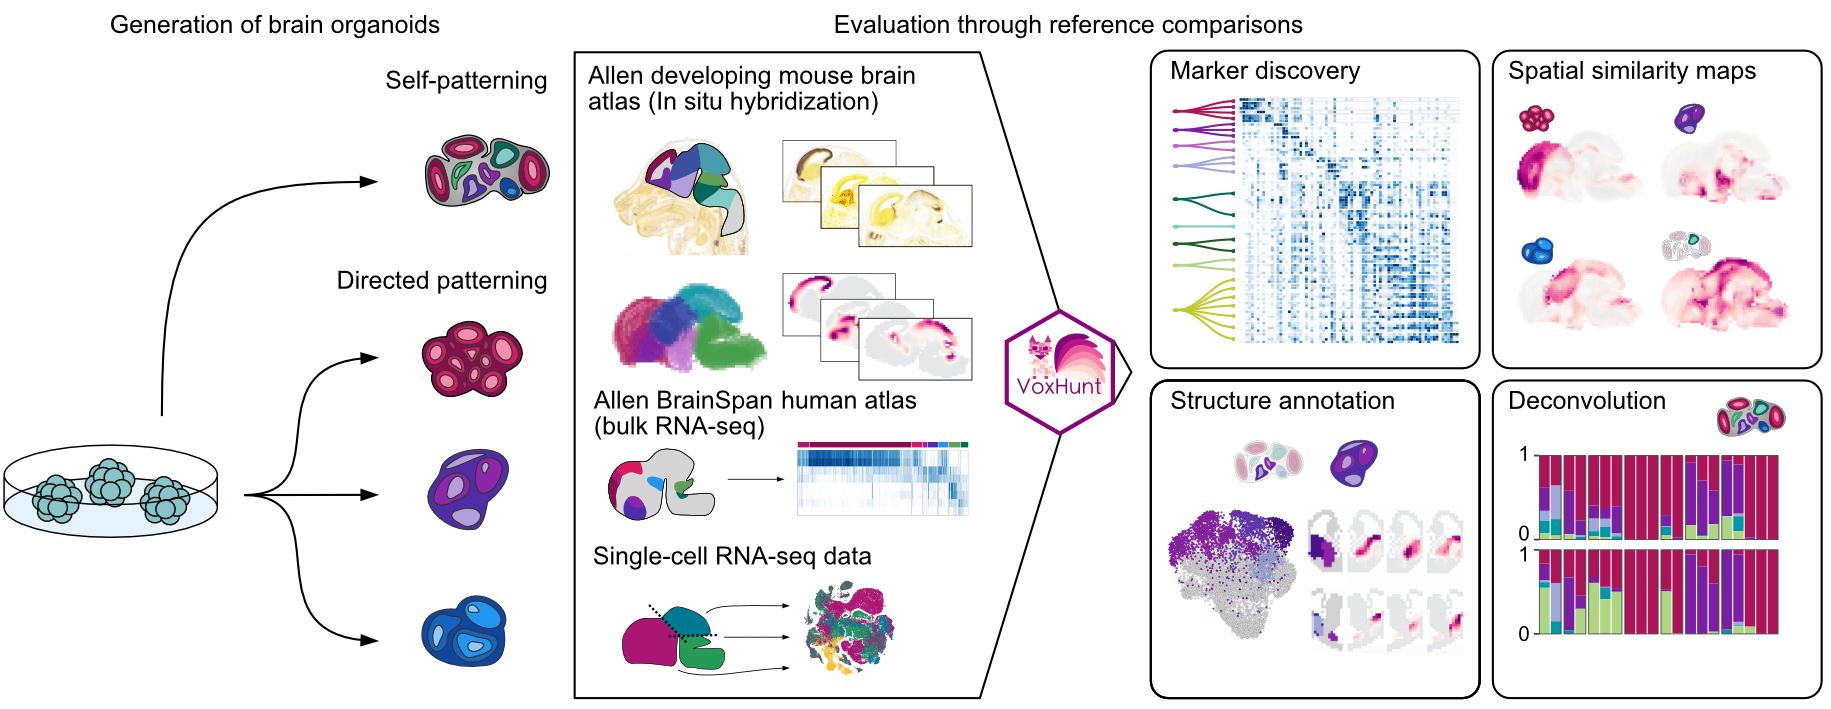
\includegraphics[width=\textwidth]{figures/voxhunt/Figure_1}
    \caption{\textbf{Overview of the VoxHunt computational toolkit for exploring heterogeneity in the developing brain and brain organoid counterparts.}
    Brain organoids generated through various protocols or patterning regimens can give rise to cells resembling different brain structures. VoxHunt helps interpret transcriptomic or epigenomic data from these organoids by providing an interface to relevant reference datasets. VoxHunt implements functions to extract brain structure markers, compute similarity maps of organoid cells, assign regional identities, and deconvolute bulk RNA-seq data into structure proportions.}
    \label{fig:vox1}
\end{figure}



\begin{figure}[t!]
    \centering
	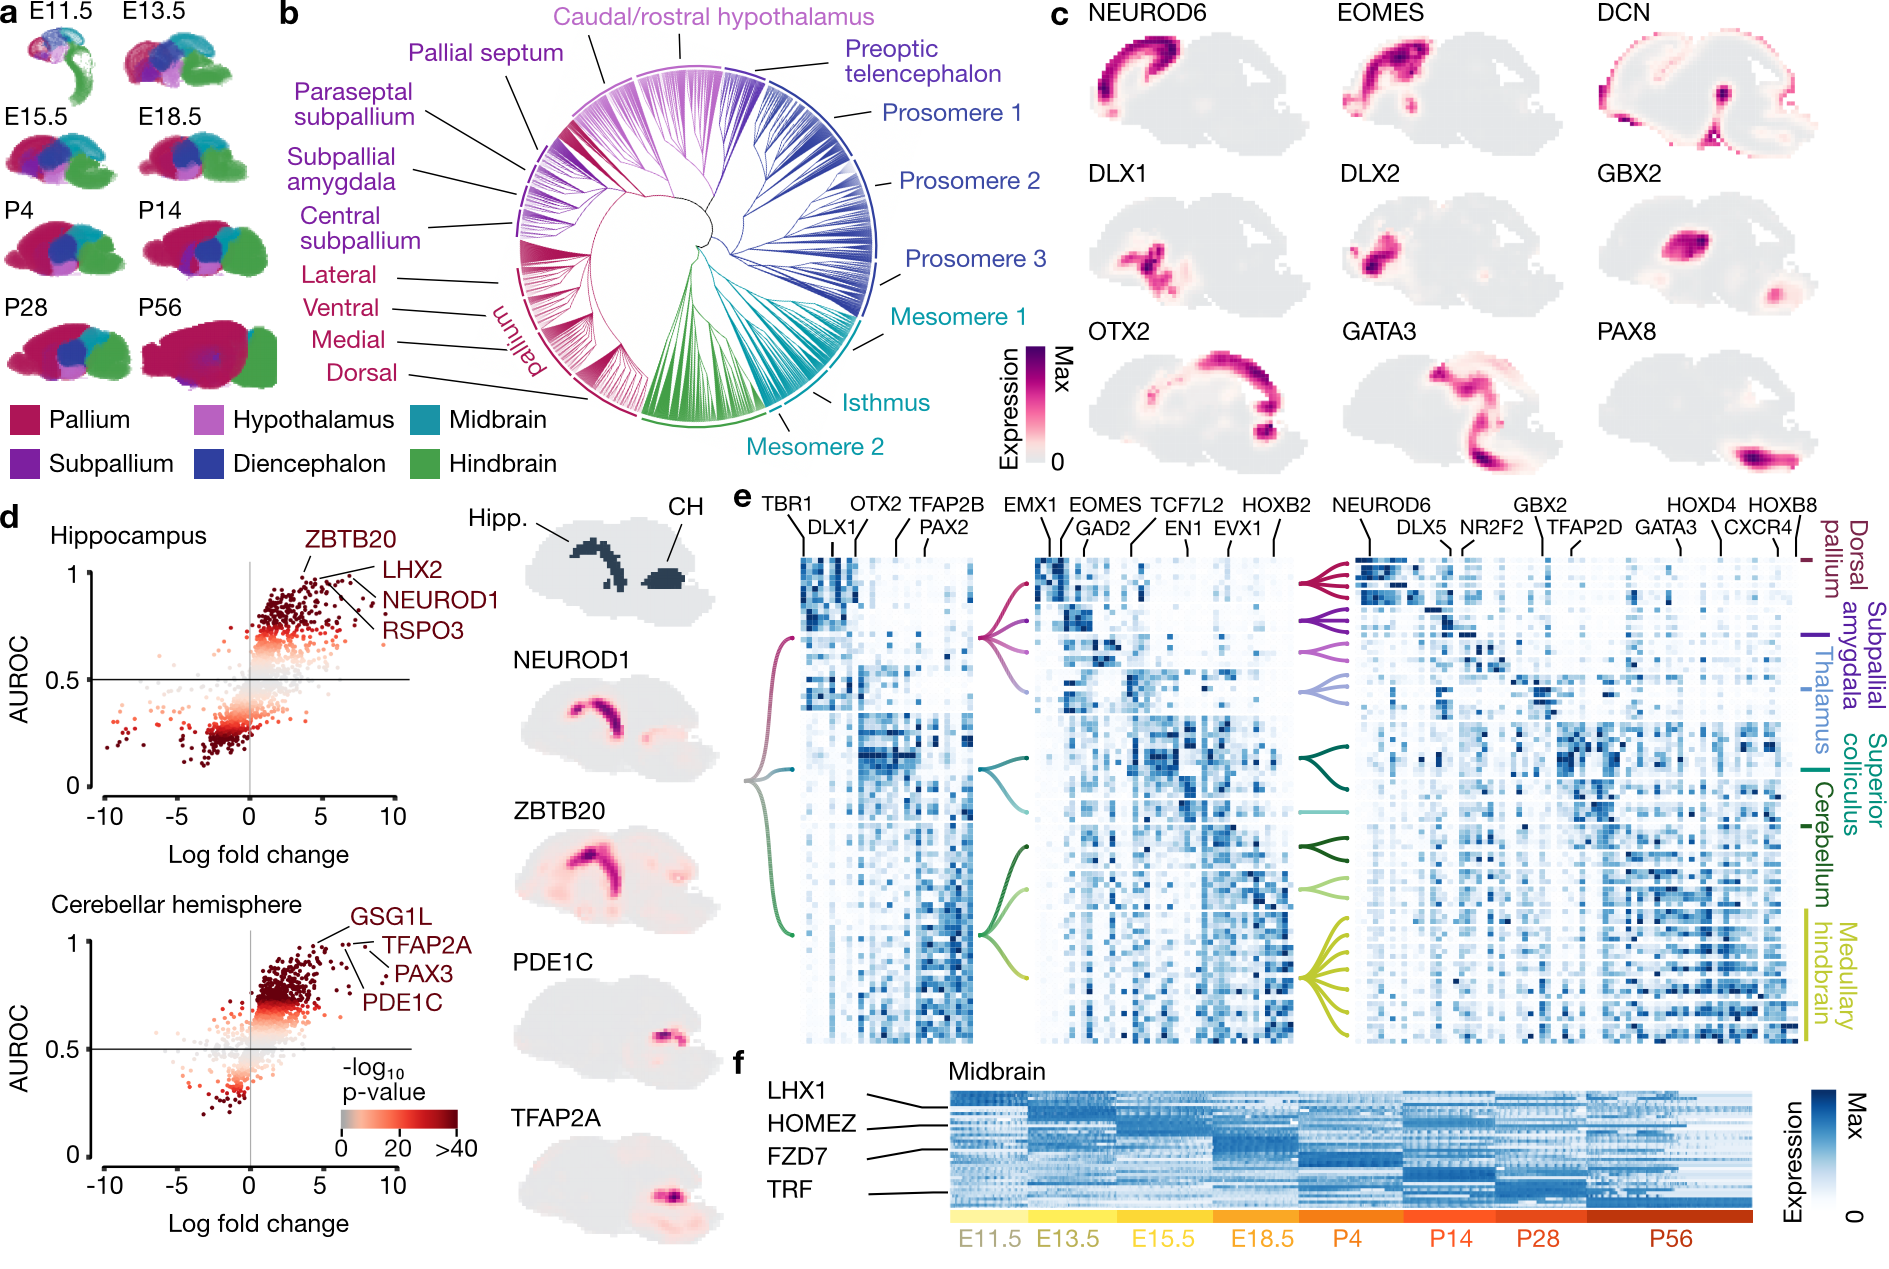
\includegraphics[width=\textwidth]{figures/voxhunt/Figure_2}
    \caption{\textbf{Feature extraction from voxel maps of developing mouse brain in situ hybridization data.} (A) Schematics show mouse brain development over time, with high-level structure annotations color-coded. (B) Dendrogram showing the hierarchically organized structure ontology from the Allen Developing Mouse Brain Atlas. (C) Spatial expression patterns of selected markers as maximum intensity projections across five central sagittal sections (8–12) in the E15.5 mouse brain. (D) Scatterplot showing feature selection for two brain structures, hippocampus (Hipp.) and cerebellar hemisphere (CH), at E15.5, together with the expression profile for the top two marker genes per structure. (E and F) Heatmap showing marker gene expression across brain structures at different levels of structure resolution at stage E15.5 (E) and across developmental stages for the midbrain (F).}
    \label{fig:vox2}
\end{figure}


\topparagraph{Brain structure marker identification}
We performed differential expression analysis between annotated brain structures and used the single-feature area under the receiver operating characteristic curve (AUROC) as a metric for selecting structure-specific genes with spatially confined expression (Figure 2.2c-d, Figure S2.1c). In this way, one can perform large-scale feature selection based on various criteria such as structure- or stage-specificity (Figure 2.2e-f, Figure S2.1d). These brain structure-enriched gene expression profiles could serve as a resource of marker genes to validate cell fate engineering and organoid protocols.


\begin{figure}[b!]
    \centering
	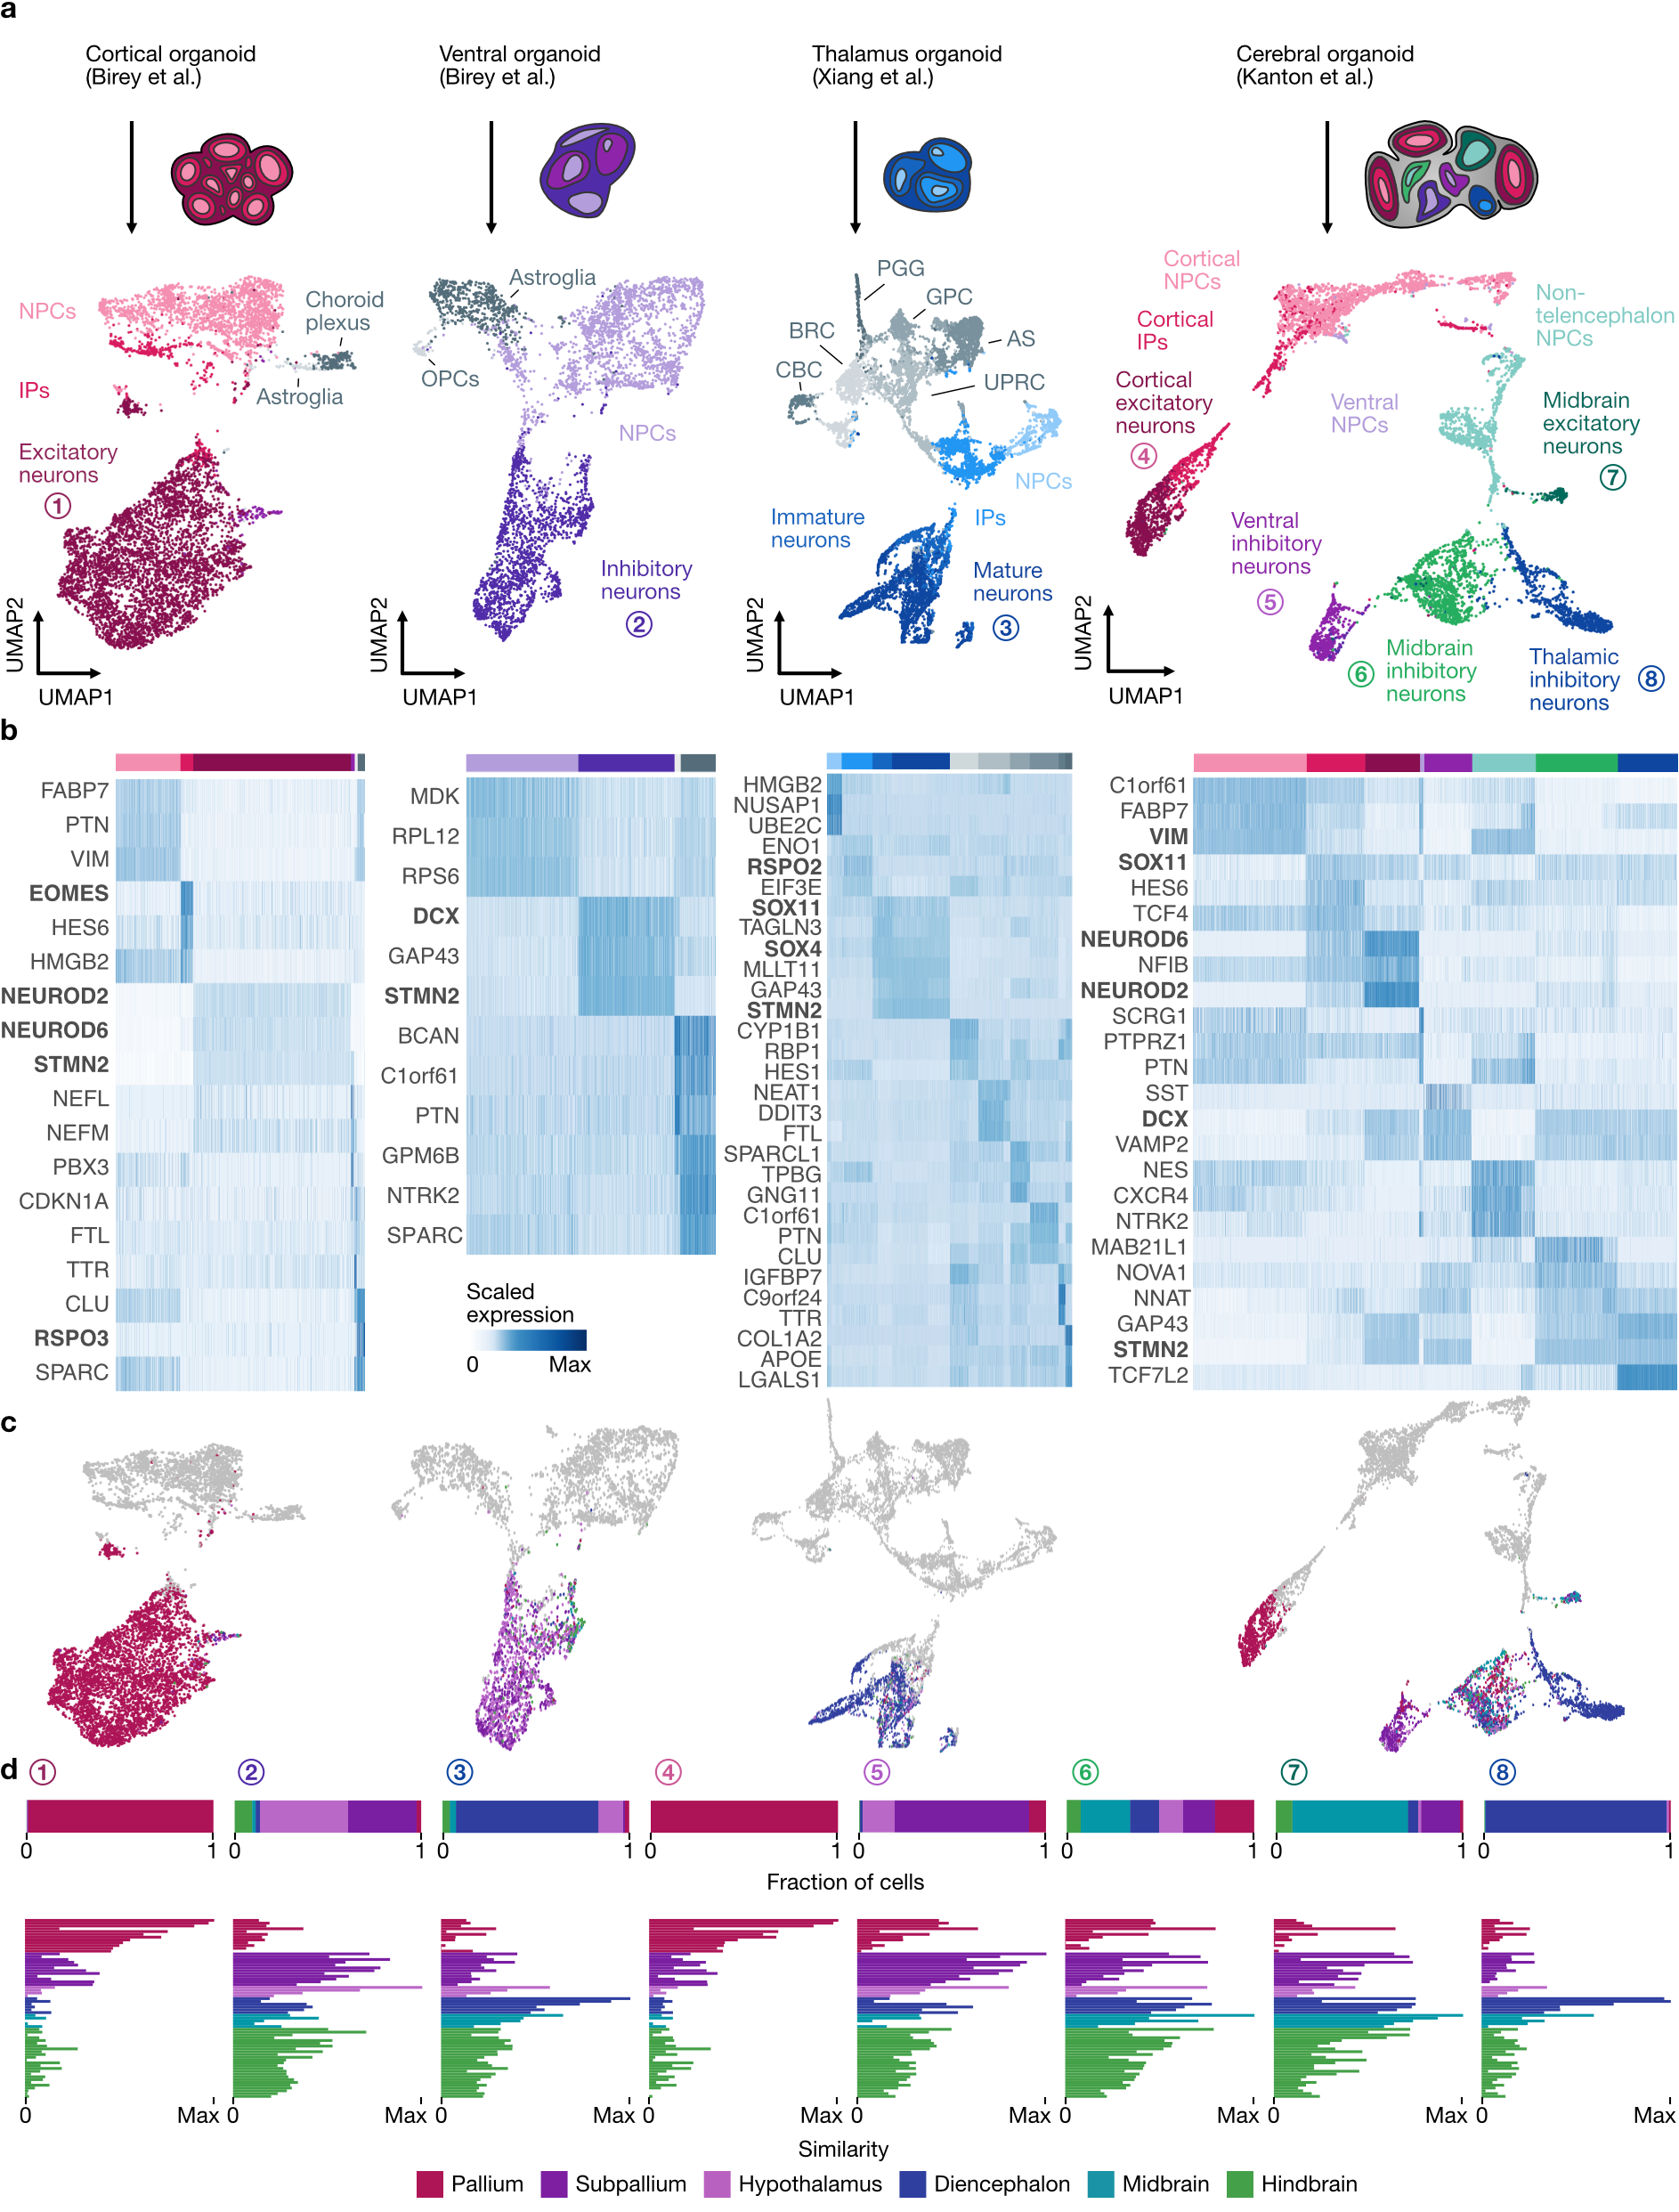
\includegraphics[width=\textwidth]{figures/voxhunt/Figure_3}
    \label{fig:vox3}
\end{figure}

\begin{figure}[t!]
    \centering
    \caption{\textbf{Single-cell transcriptomes deconstruct region composition in brain organoids} (A) UMAP projections of published single-cell transcriptome data from different organoid protocols, including cortical (Birey et al., 2017), ventral (Birey et al., 2017), thalamus (Xiang et al., 2018), and cerebral (Kanton et al., 2019). Cells are colored based on the annotations in the original publications. (B) Heatmap showing the expression of top marker genes for each cluster. Canonical marker genes are highlighted in bold. (C) UMAP projections of neuronal cells from each dataset colored by structure annotation of the voxel with maximum correlation. (D) Top: fraction of cells from each cluster annotated in (A) that have maximum correlation to each brain structure based on comparison to in situ hybridization voxel maps. Bottom: bar plots showing the mean similarity of each cluster to different brain structures. Each bar represents one brain structure at custom annotation level 4.
    IP, immediate progenitor; NPC, neural progenitor cell; OPC, oligodendrocyte progenitor cells; CBC, cilia-bearing cells; BRC, BMP-related cells; PGG, proteoglycan-expressing glia; GPC, glial progenitor cell; AS, astrocytes; UPRC, unfolded protein response-related cells.}
\end{figure}



\topparagraph{VoxHunt accurately maps reference populations}
We first validated that the mouse ISH reference atlas is a suitable resource for cell annotation of human single-cell transcriptome data. We used VoxHunt to map single-cell transcriptome data (split-pool barcoding) from the developing mouse brain (\cite{rosenberg_single-cell_2018}), which resulted in mouse-to-mouse mapping of annotated cell populations to voxelized structures (Figure S2.2a). Using this dataset, we assessed the accuracy (fraction of cells with correctly assigned structures) and contrast (similarity to second best structure/similarity to assigned structure) of the spatial mapping under different conditions for feature selection (e.g. differentially expressed genes between structures vs. most variable features), and tested the stability of structure assignments through downsampling of unique molecular identifier (UMI) in the single-cell RNA-seq data (Figure S2.2b-d). We found that accuracy was proportional to the number of features used, and this result was consistent across brain structures. However, for certain structures (e.g. pallium), contrast decreased at low or high feature inclusion. Accuracy has some dependency on UMI count, with certain structures (e.g. Rostral midbrain) being more sensitive to this aspect of the scRNA-seq data. Nonetheless, even with the relatively sparse split-pool barcoding data, we could identify optimal parameters that facilitated mapping with high accuracy and contrast. We then compared bulk RNA-seq data from microdissected human brain structures from the ABA BrainSpan Developing Human Brain Atlas (\cite{thompson_high-resolution_2014}) (S2b,c), as well as four scRNA-seq datasets from primary human brain tissues (\cite{fan_spatial_2018,nowakowski_spatiotemporal_2017,polioudakis_single-cell_2019,zhong_single-cell_2018}) (Figure S2.3). We found that each of the datasets exhibited consistently clear similarity patterns, supporting the use of mouse 4D gene expression data to match homologous brain regional data and predict properties of human cell types.



\topparagraph{Organoid region composition annotation}
We next tested if VoxHunt could be used for unsupervised annotation of cell types generated through different organoid protocols. For this, we obtained published single-cell transcriptome data from three brain structure-specific organoid protocols (thalamus, cortex, ventral telencephalon) (\cite{birey_assembly_2017,xiang_hesc-derived_2019}) as well as one cerebral (unpatterned) organoid protocol (\cite{kanton_organoid_2019}). We used Uniform Manifold Approximation and Projection (UMAP) (\cite{becht_dimensionality_2019}) embeddings to project cells onto a two-dimensional space for each protocol, and annotated the clusters as described in the original studies (Figure 2.3a). All four datasets exhibit a diversity of cell populations, including heterogeneous progenitor and neuronal cells. For neuronal cells from structure-specific organoids, successful patterning is supported by the expression of canonical marker genes (Figure 2.3b). For cerebral organoids, multiple brain structures can form in any given organoid, and marker gene expression analysis suggests the emergence of neuronal cell types from the telencephalon (pallium, subpallium), diencephalon, midbrain, and hindbrain supporting the annotations reported in the original publication (Figure 2.3b). We assessed if annotations from each dataset could be confirmed by correlating single-cell transcriptomes from each neuronal cluster with in situ expression patterns in the mammalian brain at high-level annotations that are consistent across time for telencephalon (pallium, subpallium), diencephalon, midbrain, and hindbrain (Figure 2.3c,d). Cells annotated as cortical neurons derived from both cortical or cerebral organoid protocols showed far higher correlation to pallium than to any other structure. Thalamic neurons showed a similarly clear pattern, with the majority (>90\%) of cells having the highest correlation to voxels within the diencephalon. For clusters of inhibitory neurons annotated as ventral telencephalon, we observed differences between the two organoid protocols. While cells derived from cerebral organoids had consistently higher correlation with subpallial structures, a large fraction of cells (48.3\%) from ventrally patterned organoids were most highly correlated with the hypothalamus. Cell clusters annotated as midbrain neurons derived from cerebral organoid protocols showed a noisier correlation pattern and overall lower correlation to in situ maps than any of the other clusters. While average correlation within each cluster was highest to the midbrain, correlation of single cells did not show clear agreement, especially for cluster 6 annotated as ‘midbrain excitatory neurons’.

\begin{figure}[t!]
    \centering
	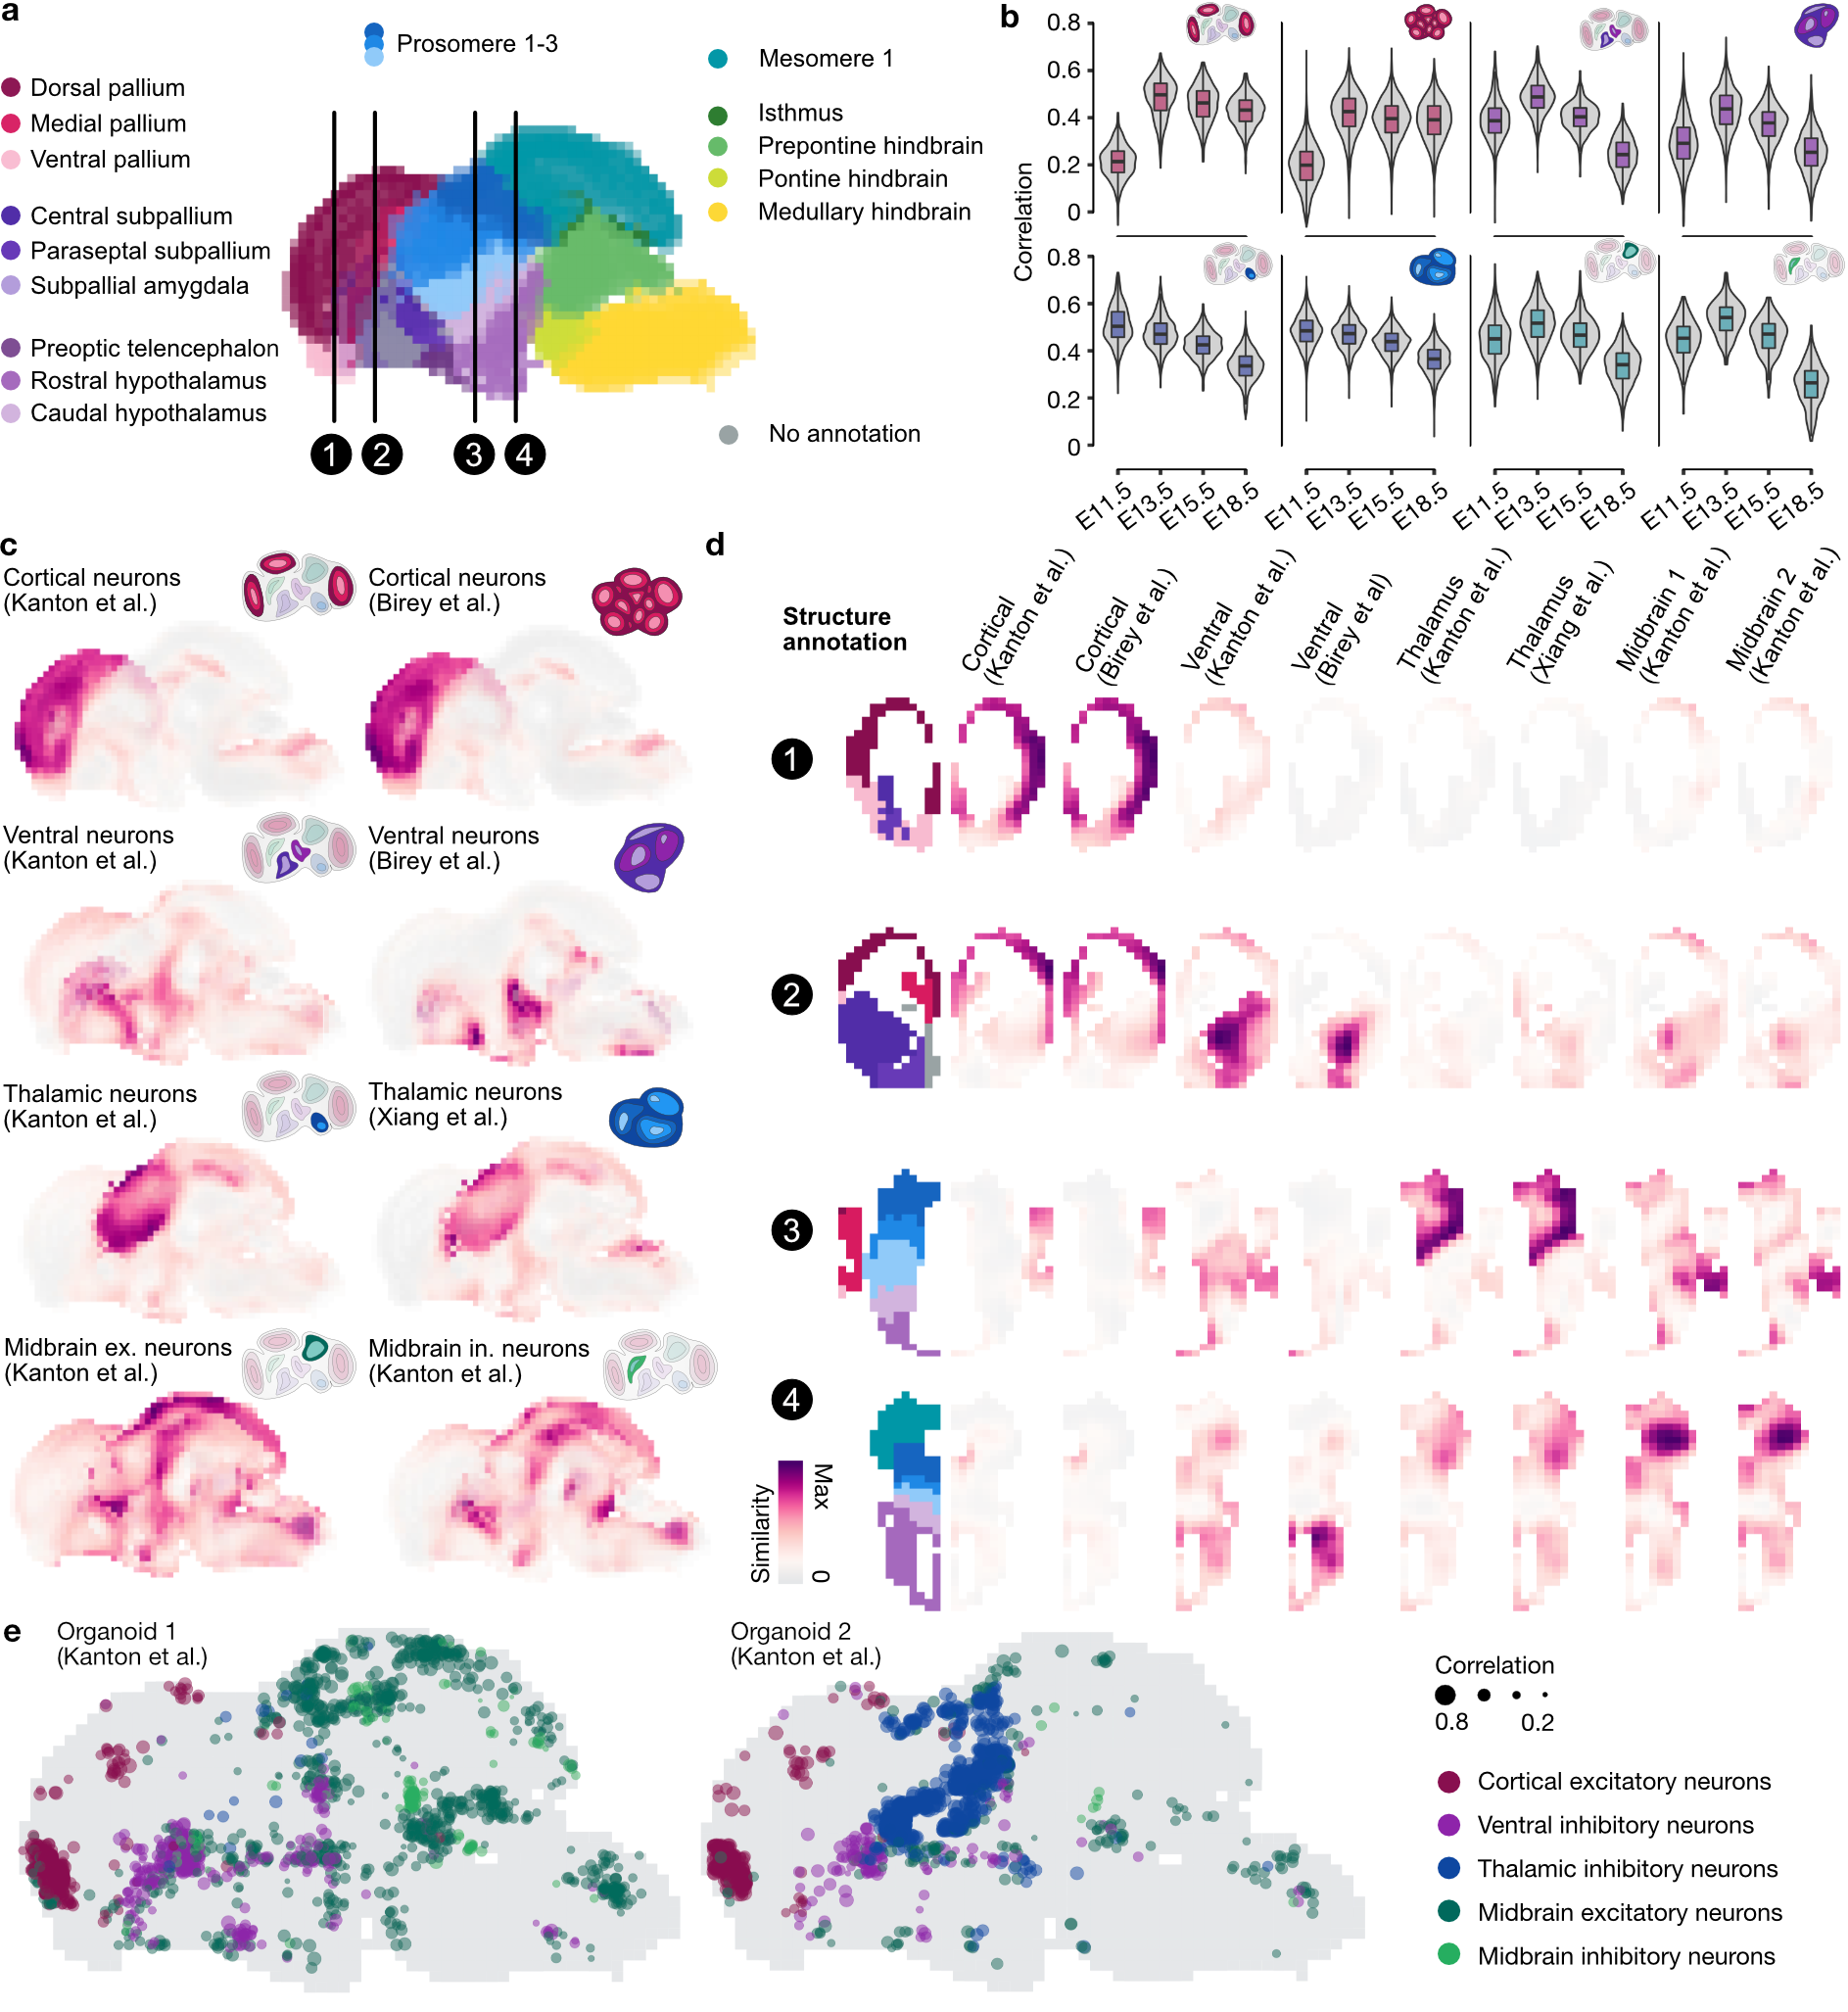
\includegraphics[width=\textwidth]{figures/voxhunt/Figure_4}
    \caption{\textbf{Comparing brain organoid cell populations to spatial brain maps.} (A) Structure annotations of the E13.5 mouse brain (sagittal view), which was used for organoid cluster annotation. Locations 1–4 are used for coronal sections shown in subsequent panels. (B) Violin plots showing the organoid cluster correlation distributions to voxel maps of the previously assigned structure (pallium, subpallium, diencephalon, and mesencephalon) across different developmental time points. (C) Sagittal projections colored by scaled similarity scores of different organoid clusters from each dataset to voxel maps of the E13.5 mouse brain. (D) Coronal sections visualizing regional annotation and scaled similarity scores to different brain structures from different clusters and protocols. (E) Sagittal view of a maximum-correlation projection of cells from two individual cerebral organoids to 8 central sections (5–12) of the E13.5 mouse brain.}
    \label{fig:vox4}
\end{figure}


\topparagraph{Spatial projection of organoid cell transcriptomes}
To select a suitable developmental stage for voxel-resolved visualization of spatial similarity patterns, we computed the correlation of each cell in a cluster to its matching structure from all fetal developmental stages (E11.5 - E18.5) (Figure 2.4a, Figure S2.4a). From the previously decomposed clusters, the majority showed the highest median correlation to E13.5, with the exception of thalamic neuron clusters, which were most highly correlated with structures at E11.5 (Figure 2.4b). For cortical neurons, we further found that their most similar developmental stage was proportional to the age of their organoid of origin (Figure S2.4b,c). For each organoid cluster, we visualized the correlation to each voxel in either a sagittal view (Figure 2.4c, Figure S2.4a) or two-dimensional coronal (Figure 2.4d) sections. To further aid the assessment of cell type compositions of individual organoids, each cell from each organoid can be projected to spatial locations within the brain based on maximum similarity to loci within the voxel maps (Figure 2.4e). These analyses reveal the spatial location within the brain tissue where each cluster or cell has maximal correlation, which can be used to assess the specificity of the regional neuronal population and help annotate previously unknown cell populations. Similarity patterns can also be explored in three-dimensional registrations of the voxel maps (Supplementary Videos 2.1-2.5). 

\topparagraph{Complementary reference datasets as high-dimensional search spaces}
To test whether the structure annotations obtained from mapping to ISH data could be further enhanced through other reference datasets, we compared organoid-derived neurons to time course bulk RNA-seq data from the human brain (BrainSpan) (\cite{thompson_high-resolution_2014}) (Figure S2.4d) as well as a single-cell transcriptomic atlas of the developing mouse brain (\cite{la_manno_molecular_2021}) (Figure S2.4e). Similarities of neuronal clusters to BrainSpan samples largely agreed with the comparison to ISH data. However, BrainSpan covers a limited number of brain structures and lacks midbrain samples, which makes it unsuitable for annotating neurons from certain protocols. The single cell atlas of the developing mouse brain provides coarse (forebrain, midbrain, hindbrain; Figure S2.4e) annotations of cell types arising during early mammalian brain development, and provides functional annotations which cannot be derived from the ISH data alone. We found that organoid-derived cortical neurons showed the highest similarity to excitatory neurons, while ventral neurons mapped to inhibitory (GABA-ergic) neurons, which is in line with expectations (Figure S2.4f). Comprehensive whole brain scRNA-seq datasets from human and mouse will be valuable references for functionally annotating neuronal and non-neuronal cell types.

\topparagraph{Assessing region specificity across organoid protocols}
We used VoxHunt to assess cell identities generated in organoids from different protocols. We analyzed scRNA-seq data from 9 different organoid protocols (\cite{bhaduri_cell_2020,birey_assembly_2017,giandomenico_cerebral_2019,kanton_organoid_2019,pellegrini_human_2020,pollen_establishing_2019,velasco_individual_2019,xiang_hesc-derived_2019}) that have been reported to generate diverse neuronal populations. We found that spatial similarity maps and assigned region identities by VoxHunt corresponded well with the original annotations (Figure S2.5). We found that choroid plexus (ChP) cells from central nervous system barrier forming organoids (\cite{pellegrini_human_2020}) showed a distinct correlation to the roof plate of the invaginated telencephalic vesicle, a ChP precursor. In some cases, VoxHunt enabled annotation of neuronal cell populations with a previously uncertain identity. For example, we observed that neurons in ChP organoids mapped distinctly to diencephalon structures, and appear distinct from neurons generated through a telencephalic organoid protocol (Figure S2.5i). We also observed substantial brain region composition heterogeneity between individual cerebral organoids consistent with previous reports (\cite{kanton_organoid_2019}), especially when comparing organoids from different human iPSC lines (Figure S2.5j). In comparison, the majority of cells from the dorsal forebrain organoid model match pallial structures across organoids and iPSC lines. We note that we were able to annotate a previously unknown cluster present in 1 month old cerebral organoids (\cite{camp_human_2015}) (Figure S2.6a,b). This population was marked by RSPO2/3 and WNT2B which localizes to the invaginated telencephalic roof plate (\cite{kamata_r-spondin_2004}) and transient structures annotated as pallium at the boundary of the developing telencephalon and diencephalon (Figure S2.6c-e). 


\begin{figure}[b!]
    \centering
	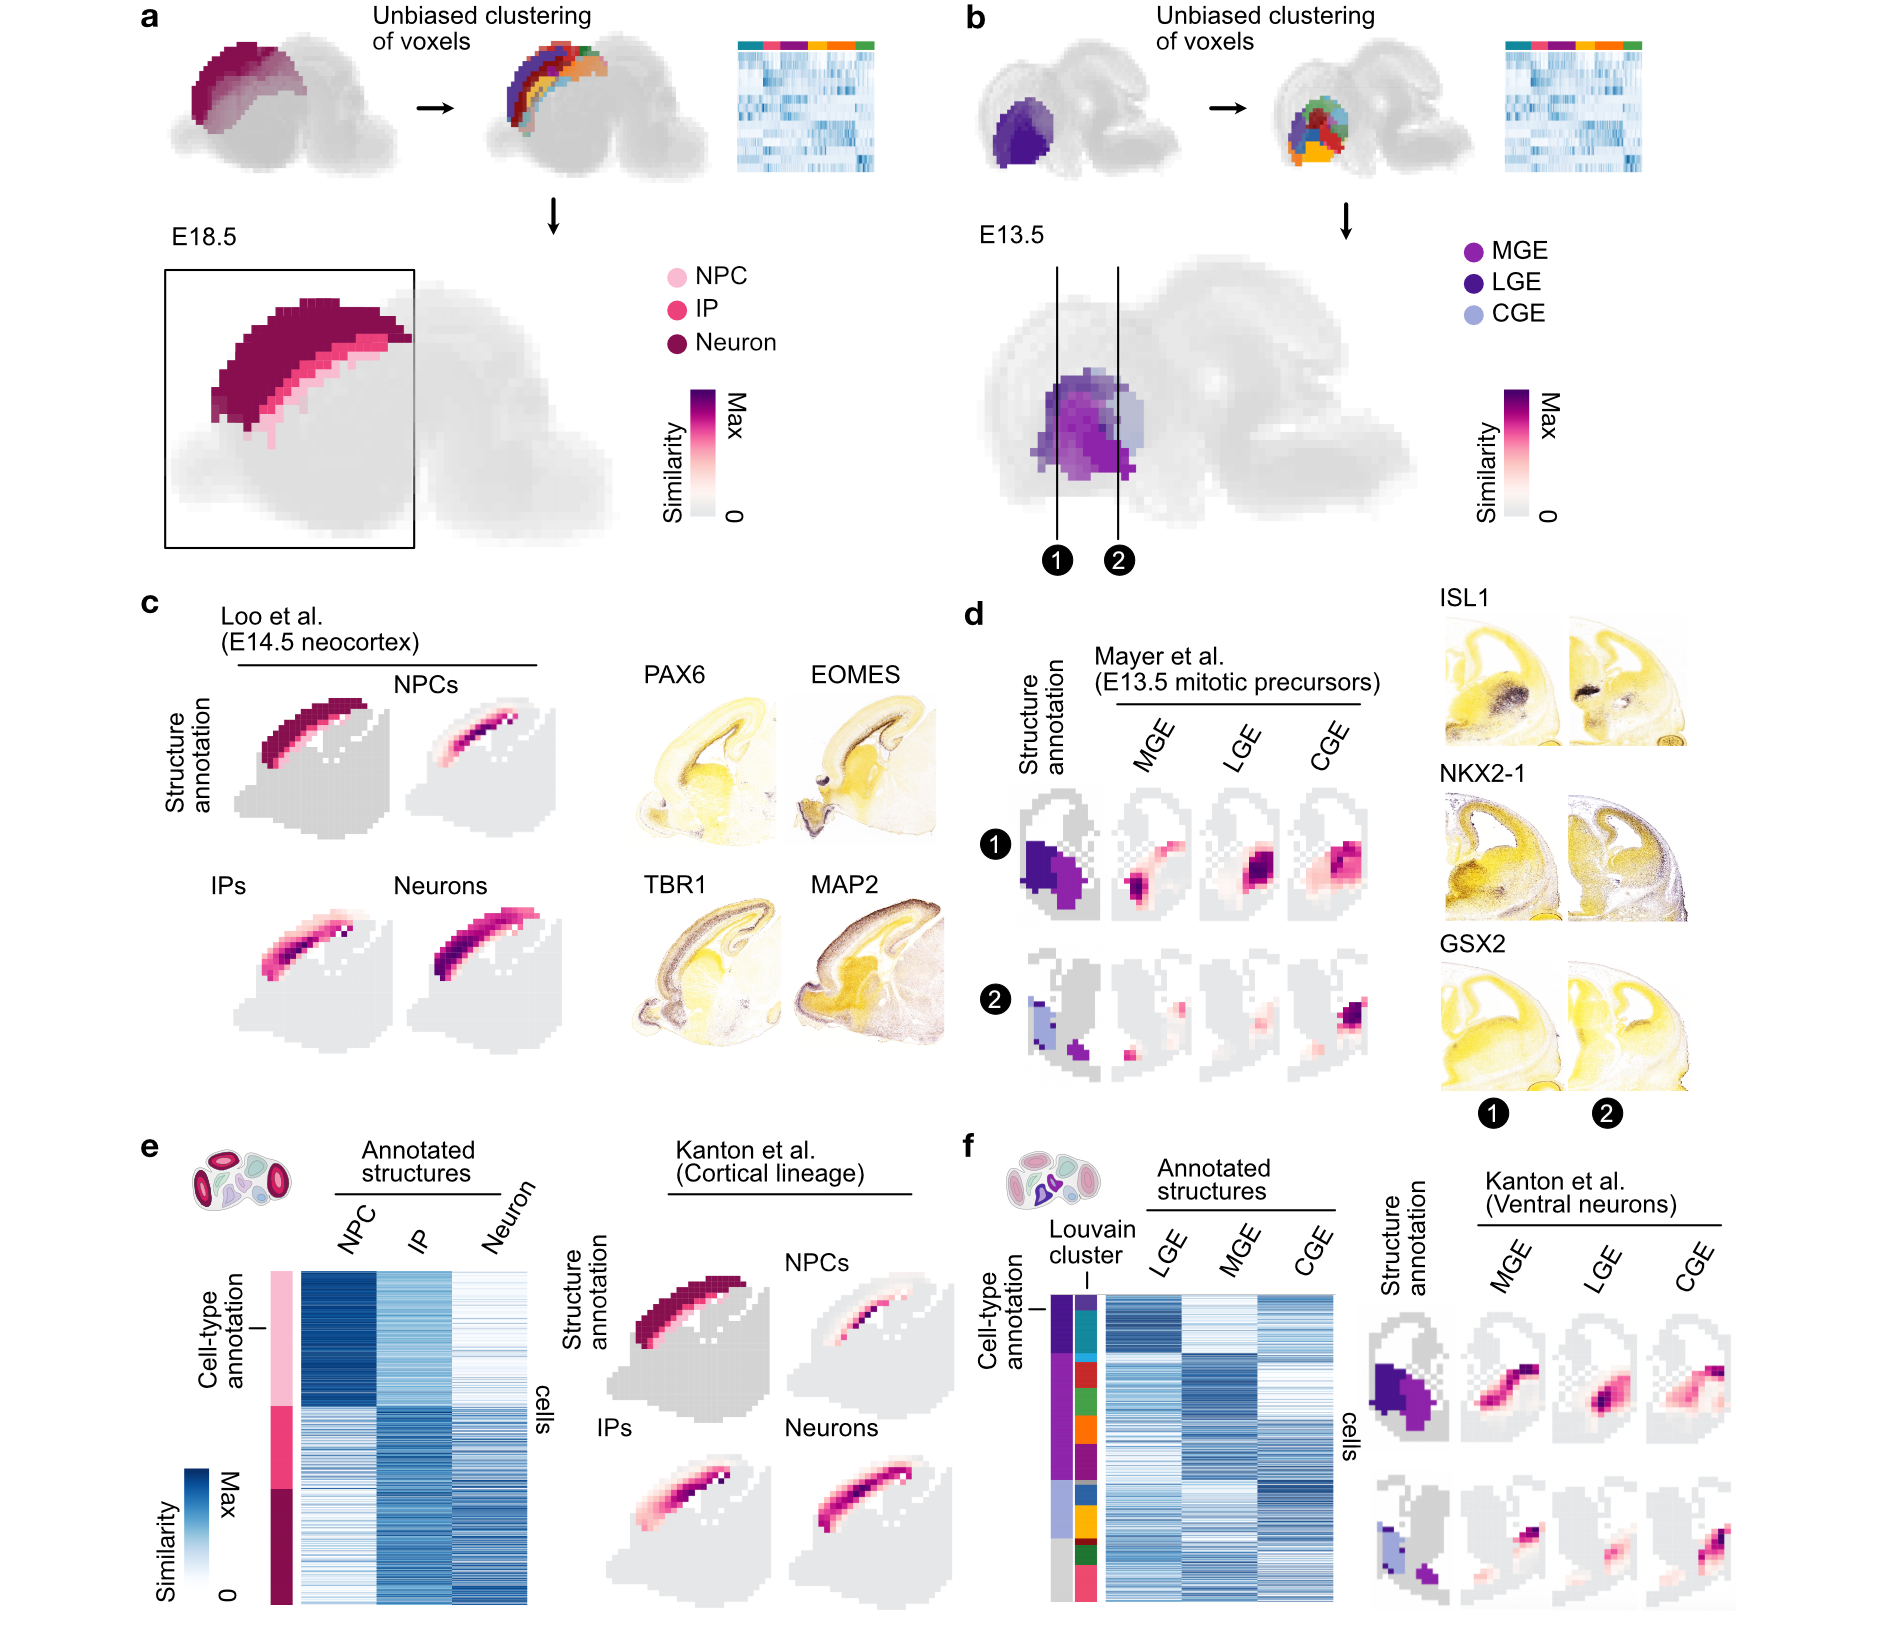
\includegraphics[width=\textwidth]{figures/voxhunt/Figure_5}
    \caption{\textbf{Substructure resolution of transcriptomic maps.} (A and B) Schematic of substructure annotation. Unbiased clusters of voxels were annotated based on the expression of canonical marker genes to identify fine structures beyond existing annotations in the dorsal (A) and ventral (B) telencephalon. (C) Left: sagittal sections visualizing custom substructure annotations and scaled similarity scores from E14.5 mouse neocortex NPC, IP, and neuron primary scRNA-seq data to voxel maps of the E18.5 mouse brain. Right: ISH images of marker gene expression in shown sections. (D) Left: coronal sections visualizing custom substructure annotations and scaled similarity scores from E13.5 mouse mitotic precursors from LGE, MGE, and CGE primary scRNA-seq data (Mayer et al., 2018) to voxel maps of the E13.5 mouse brain. Right: E13.5 mouse ISH images of marker gene expression in shown sections. (E) Left: heatmap showing similarities of cortical cells from cerebral organoids (Kanton et al., 2019) to annotated substructures. Right: coronal sections visualizing custom annotations and scaled similarity scores from organoid cell states to voxel maps of the E13.5 mouse brain. LGE, MGE, and CGE, lateral, medial, and caudal ganglionic eminence; NPC, neural progenitor cell; IP, immediate progenitor. (F) Left: heatmap showing similarities of ventral neurons from cerebral organoids (Kanton et al., 2019) to annotated substructures and their resulting annotations. Right: coronal sections visualizing custom annotations and scaled similarity scores from organoid ventral neuron populations to voxel maps of the E13.5 mouse brain.}
    \label{fig:vox5}
\end{figure}


\topparagraph{Annotating organoid cell identity at substructure resolution}
We were curious if we could go beyond the structure ontology provided by the ABA to reveal a higher-resolved annotation of organoid cell types. For this, we selected two high-level structures, the dorsal pallium and the subpallium and performed unbiased clustering on voxel transcriptomes (Figure 2.5a,b). We aggregated these clusters based on the expression of canonical marker genes to reveal neural progenitor cell (NPC), immediate progenitor (IP) and neuronal layers in the dorsal pallium and the lateral, medial and caudal ganglionic eminences (LGE, MGE, CGE) in the subpallium. These custom annotations matched the correlation patterns of single-cell transcriptomic data derived from the annotated structures in mice (\cite{loo_single-cell_2019,mayer_developmental_2018}) as well as the expected anatomic position and morphology (Figure 2.5c,d). We found that organoid cells from the cortical trajectory clearly mapped onto the annotated pallial zones (Figure 2.5e). Moreover, ventral neuron clusters from cerebral organoids could be clearly annotated as LGE, MGE or CGE-like interneurons based on their similarities to the substructures (Figure 2.5f). We further used these newly annotated subpallial structures to resolve and compare the heterogeneity of inhibitory neurons derived from three organoid protocols (\cite{birey_assembly_2017,kanton_organoid_2019,xiang_hesc-derived_2019}). We found that all protocols gave rise to diverse neuronal populations, some of which matched distinct subpallial structures (Figure S2.6g-m), while others were more similar to the hypothalamus and did not express any canonical GE marker genes (Figure S2.5g,h). We note that these results may be confounded by maturation differences and further analysis would benefit from availability of time course data from human samples. Nevertheless, this data demonstrates that comparison to spatially resolved reference atlases can elucidate previously unappreciated and biologically meaningful heterogeneity within brain organoids.


\begin{figure}[b!]
    \centering
	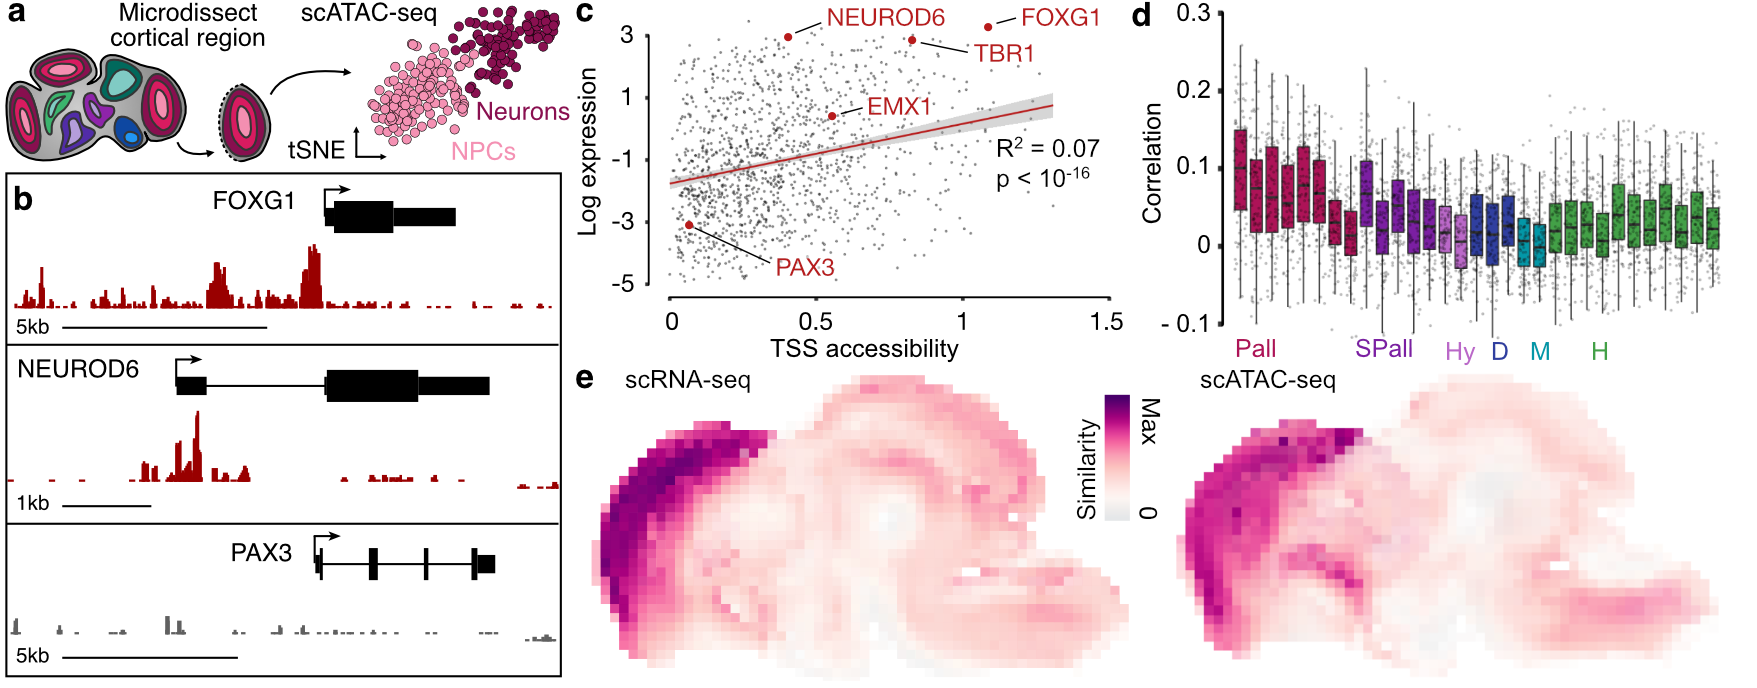
\includegraphics[width=\textwidth]{figures/voxhunt/Figure_6}
    \caption{\textbf{Projecting chromatin accessibility profiles to spatial brain maps.} (A) Single-cell RNA-seq (Camp et al., 2015; Kanton et al., 2019) and single-cell ATAC-seq (Kanton et al., 2019) was performed on single cortical regions microdissected from cerebral organoids between 2 and 4 months of age. (B) Signal tracks showing accessibility (normalized read count) at the transcription start site (TSS) of the forebrain marker FOXG1, the cortex neuron marker NEUROD6, and the hindbrain marker PAX3. (C) Expression of all measured genes in the E13.5 pallium (cortex) as a function of TSS accessibility in cortical organoid cells. The fit of a linear model is indicated in red, the gray area shows the standard error, and the indicated p-value was obtained through an F-test. (D) Boxplots showing Pearson correlation distributions of organoid TSS accessibility (log-normalized peak count) to gene expression in different brain structures. (E) Sagittal projections of the E13.5 mouse brain colored by scaled similarity scores of organoid TSS accessibility (scATAC-seq) or expression (scRNA-seq) with voxel map expression of the downstream gene. Pall, pallium; SPall, subpallium; Hy, hypothalamus; D, diencephalon; M, midbrain; H, hindbrain.}
    \label{fig:vox6}
\end{figure}



\topparagraph{Spatial mapping of chromatin accessibility data}
Next, we show that similar analyses can be performed for single-cell ATAC-seq (Assay for Transposase-Accessible Chromatin using sequencing) data. In this case, we obtained paired scATAC-seq and scRNA-seq data performed on the same cell suspension generated from micro-dissected regions from 2-4 month cerebral organoids (\cite{kanton_organoid_2019}) (Figure 2.6a). We determined accessibility scores at the transcription start site (TSS) of each gene measured in the in situ hybridization atlas (Figure 2.6b), and then calculated TSS access and expression correlation across each structure annotated in the voxel map (Figure 2.6c,d). Coloration of the 3D voxel map based on correlation revealed that both transcriptomes and chromatin accessibility scores of neuronal cells from the micro-dissected region have the highest correlation with the developing cortex (Figure 2.6e). This demonstrates that VoxHunt can annotate cells across multiple single-cell -omics modalities.

\topparagraph{Reference-based deconvolution of organoid bulk transcriptomes}
There are on-going efforts to steer brain organoid development toward distinct regional identities by supplying cues in defined culture conditions. Whole organoid bulk transcriptome measurements provide a high-information content metric of organoid states at relative low cost and high throughput. Therefore, we established a framework within VoxHunt to assess organoid brain structure representation using bulk transcriptomics. The pseudo-bulk data can be accurately deconvoluted into proportions of brain regions that are represented within heterogeneous cerebral organoids, and this is further validated with data from directed patterning into cortex or thalamus (Figure S2.7a,b). We note that this approach is particularly powerful at organoid stages where neurons are abundant, as neurons harbor strong structure-specific multi-gene signatures.


\topparagraph{Assessing organoid patterning using multiplexed transcriptomics and reference mapping}
Finally, we highlight how reference-mapping organoid transcriptomes can be used to assess the outcome of culture condition manipulations. We performed a proof of principle experiment where we incubated developing organoids with several different patterning molecules including R-spondin (RSPO) 2, RSPO 3, sonic hedgehog (SHH), an activator of the Wnt pathway (CHIR99021), and two small molecules for dual SMAD inhibition (SB431542, Dorsomorphin) (Figure 2.7a; S7c). We generated organoids in a multi-well plate and performed bulk RNA sequencing of multiple individual organoids after transient treatment with two concentrations of each of these molecules, as well as control untreated organoids, resulting in 61 total bulk transcriptome measurements. Principal component analysis (PCA) showed transcriptome heterogeneity induced by morphogen treatment that were largely consistent across organoids for a given condition (Figure 2.7b). Next, we correlated each bulk transcriptome to each voxel within the ABA developing mouse brain reference (E11.5), and found variation between conditions that was consistent across organoids for a given condition (Figure 2.7c). Interestingly, we found that RSPO2 and RSPO3 conditions had similar and reproducible patterns with enriched mapping to a particular location within the developing brain. As noted above, RSPO2/3 expression localizes to the invaginated telencephalic roof plate (\cite{kamata_r-spondin_2004}) and transient structures annotated as pallium at the boundary of the developing telencephalon and diencephalon (Figure S2.6d,e). The RSPO2/3-induced signature in organoids was distinct from control organoids as assessed through PCA and differential expression analysis (Figure 2.7b,d-e). The locations with highest mapping of the RSPO2/3 treated organoids were voxels adjacent to where both of these genes are highly and specifically expressed in the developing brain (Figure 2.7f,h). In addition, many genes that are differentially expressed between control and RSPO2/3- treated organoids are also expressed in voxels adjacent to the RSPO2/3 positive location, including choroid plexus markers TTR, CLU, and HTR2C (Figure 2.7f-h). It is unclear how RSPO2/3 might induce choroid plexus formation, and known R-spondin receptors such as Leucine-rich repeat-containing G-protein-coupled receptors (LGRs) are not probed for in the ABA. Nonetheless, this data provides a potential hint into how local morphogen expression within the developing brain might impact the development of cell phenotypes within neighboring structures. Altogether, this experiment provides an experimental and computational strategy for modulating and assessing developing brain organoids in high-throughput through transcriptome sequencing and reference atlas comparison.


\begin{figure}[t!]
    \centering
	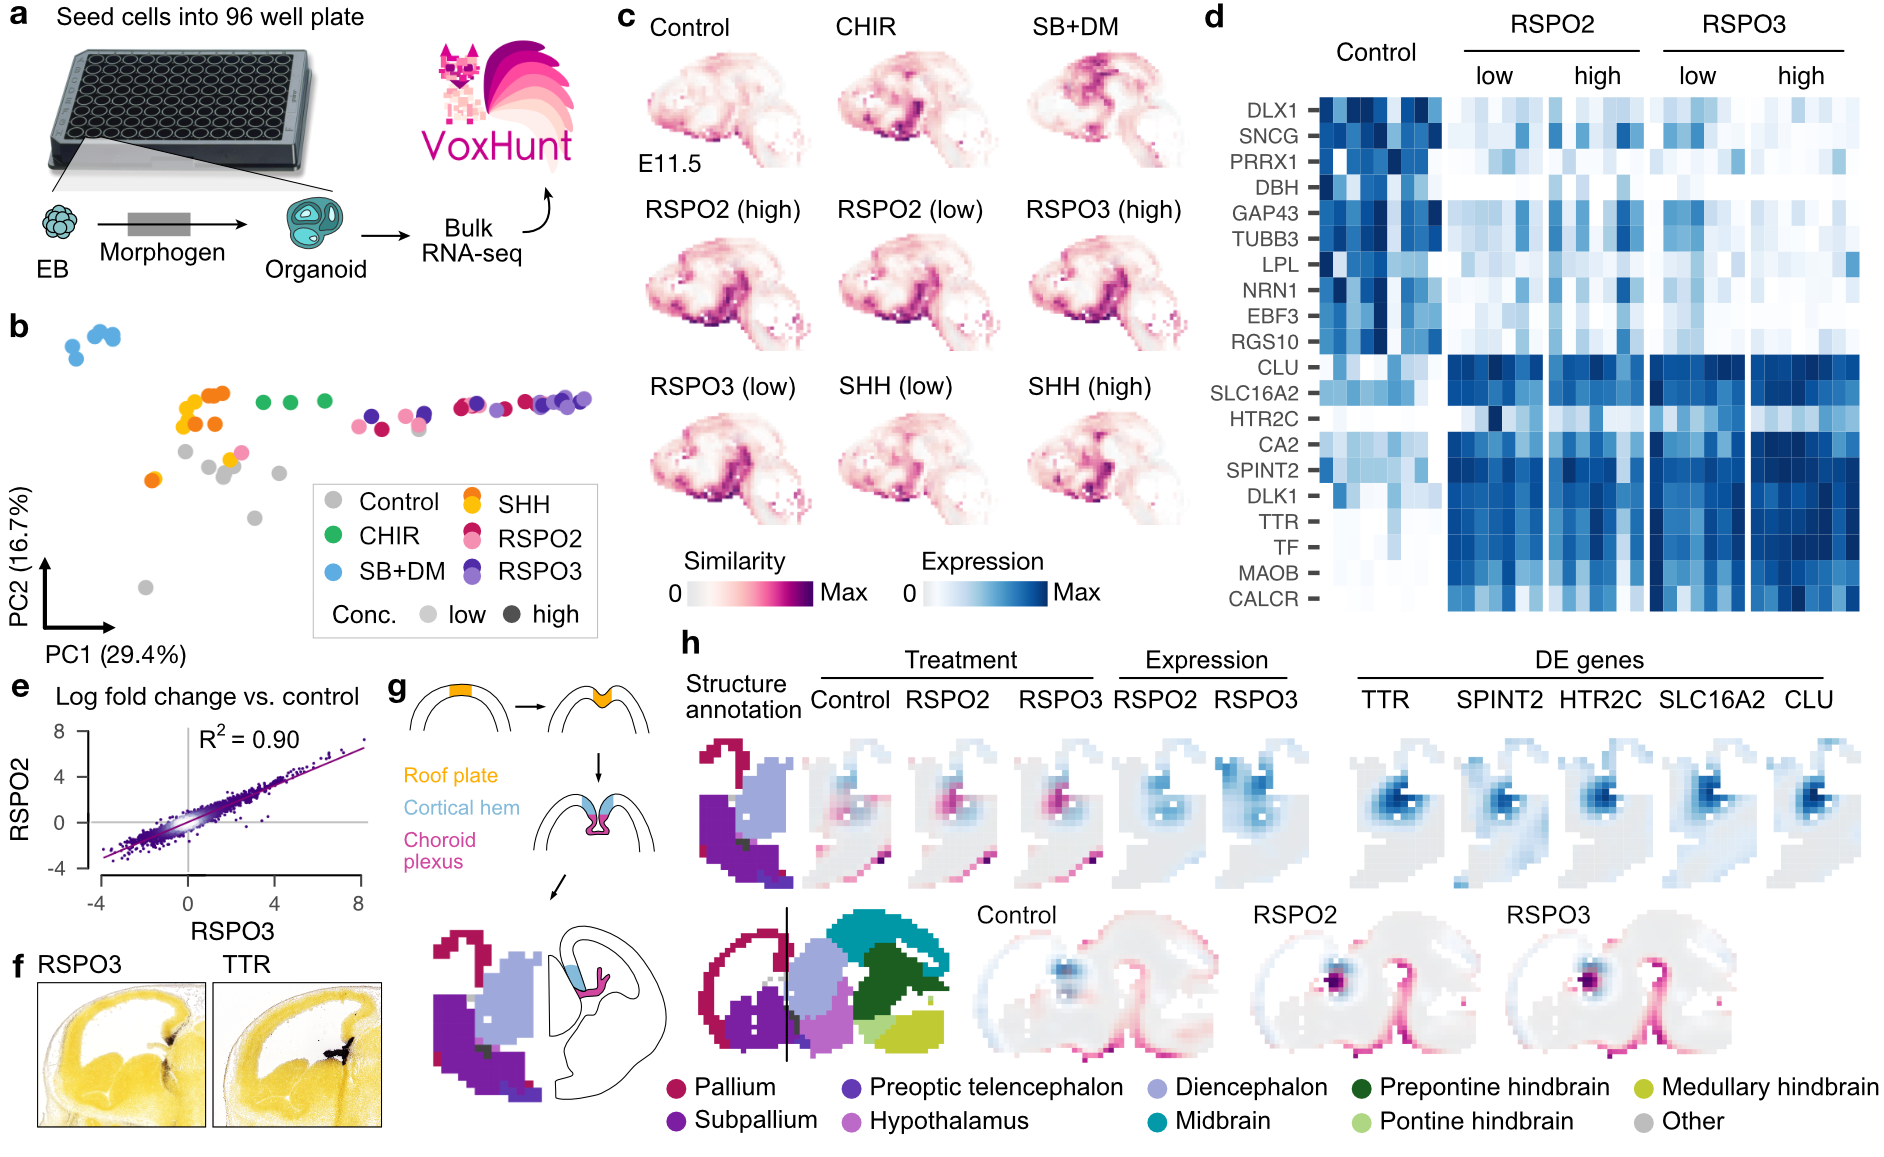
\includegraphics[width=\textwidth]{figures/voxhunt/Figure_7}
    \caption{\textbf{Assessing the effects of morphogens on brain organoids using multiplexed bulk transcriptomics.} (A) Schematic of the experimental setup. Single developing organoids were exposed to different morphogens in a 96-well plate. Bulk RNA-seq libraries were prepared from each organoid and multiplexed for sequencing. (B) First two principal components of organoid transcriptomes. Each point represents one individual organoid and is colored by condition. (C) Spatial similarity maps of each condition to the E11.5 developing mouse brain ISH atlas. (D) Heatmap showing the expression of differentially expressed genes between control and R-spondin conditions.(E) Correlation of transcriptomic effect sizes (log fold change) for RSPO2 and RSPO3 conditions compared to control samples. (F) In situ hybridization images of RSPO3 and the choroid plexus marker TTR in coronal sections of E13.5 mouse brain. (G) Schematic of roof plate invagination and early stages of choroid plexus development. (H) Top left: coronal sections visualizing regional annotation and scaled similarity scores overlaid with RSPO3 expression for control and R-spondin conditions. Top right: coronal sections visualizing expression of differentially expressed genes between control and R-spondin conditions. Bottom: sagittal sections visualizing the regional annotation and scaled similarity scores overlaid with RSPO3 expression for control and R-spondin conditions.}
    \label{fig:vox7}
\end{figure}



\subsection{Discussion}
Here we have developed a set of computational tools that enables researchers to quickly and flexibly explore the vast amount of data within the Allen Brain Atlas and other brain reference resources. We provide multiple examples for how these tools can be implemented to interpret single-cell genomic data from 3D brain tissue cultures through systematic comparison to these references. There are still many uncertainties about how to effectively generate brain structures from humans and other species in vitro. VoxHunt \href{https://github.com/quadbiolab/voxhunt}{https://github.com/quadbiolab/voxhunt} will be a powerful approach to assess organoid engineering protocols, to annotate cell fates that emerge in organoids during genetic and environmental perturbation experiments, and to develop data-driven hypotheses about the mechanisms underlying mammalian brain patterning that can be tested in vitro. 

\topparagraph{Limitations of the study}
One major limitation with the current VoxHunt implementation is that the most comprehensive brain transcriptome atlases have been generated using mouse brain tissue. The human brain has evolved features that are different from other mammals and primates, and there are certain scenarios where comparison to non-human tissues may be inadequate. In addition, single-cell sequencing has illuminated a great diversity of molecularly distinct neuronal and non-neuronal states in the brain, which is partially recapitulated in engineered human brain tissues. However, there is not yet a comprehensive spatial reference with single cell resolution across the entire brain to use a query space for organoid-reference comparisons. High-resolution 4D reference brain maps will serve as valuable resources for unbiased and high-dimensional search spaces, and VoxHunt will be an important tool to explore and interpret bulk and single-cell sequencing data from brain organoid systems. 


\subsection{Methods}

\paragraph{Acknowledgments}
We thank the Treutlein and Camp labs for helpful discussions and Sophie Jansen and Ryoko Okamoto for experimental support. We also want to thank the Kirkeby lab for kindly sharing the NKX2.1GFP/w cell line. This project was made possible in part by the Chan Zuckerberg Initiative DAF (grant CZF2017-173814 to J.G.C. and B.T.), a Silicon Valley Community Foundation advised fund, the European Research Council (Anthropoid-803441 to J.G.C. and Organomics-758877 and Braintime-874606 to B.T.), the Swiss National Science Foundation (project grant 310030\_84795 to J.G.C. and project grant 310030\_192604 to B.T.), and the National Center of Competence in Research, Molecular Systems Engineering. J.S.F. was supported by a Ph.D. fellowship of the Boehringer Ingelheim Fonds.

\paragraph{Author contributions}
J.S.F. developed the computational tool and performed computational analyses with support from Z.H. and M.J.B. F.S.C. designed and executed the patterning experiment with assistance from M.S. J.S.F., F.S.-C., B.T., and J.G.C. designed the study and wrote the manuscript.

\paragraph{Declaration of interests}
B.T. is a member of the Cell Stem Cell advisory board.

\paragraph{Data and code availability}
VoxHunt was implemented as an R package and is available at\\\href{https://github.com/quadbiolab/voxhunt}{https://github.com/quadbiolab/voxhunt}. \\
R markdown scripts reproducing the main analyses in study are available at\\ 
\href{https://github.com/quadbiolab/voxhunt_reproducibility}{https://github.com/quadbiolab/voxhunt\_reproducibility}.\\
All datasets used in this study are available for download in public repositories (see Key Resources Table for individual accession numbers). 

\paragraph{Materials availability}
HES3, NKX2.1GFP/w hESCs will be provided upon execution of a suitable Materials Transfer Agreement (MTA) with Ed Stanley and Andrew G. Elefanty (Murdoch Childrens Research Institute, Melbourne).

\paragraph{hESC experiments approval}
Stem cell experiments with NKX2.1GFP/w hESCs were approved by the Bundesamt für Gesundheit (Swiss Health Federal Office) with disposition number 606.0000-1/31 / 19.018224; and by the Ethikkommission Nordwest- und Zentralschweiz (Ethics Commision for Northern and Central Switzerland)

\paragraph{hESC Line Culture and Maintenance}
NKX2.1GFP/w hESCs were obtained from Agnete Kirkeby’s research group at the University of Copenhagen, after arrangement of an MTA with Ed Stanley and Andrew G. Elefanty (Murdoch Childrens Research Institute, Melbourne). NKX2.1GFP/w hESCs were grown at 37oC, 5\% CO2 in feeder-free conditions, on 6-well tissue culture plates coated with hESC-Qualified Matrigel (Corning). hESCs were fed every other day with mTesR Plus (StemCell Technologies) and passaged when reaching around 80\% confluence with EDTA for gentle dissociation. NKX2.1GFP/w hESCs were tested at passage 67 for copy number changes using the Agilent ISCA 8x60K v2 array and no abnormalities were detected. Cells were also karyotyped at passage 78 and showed apparently normal female karyotype in 20 cells examined. These analyses were performed by the Cell Guidance Systems Genetics Service (Cambridge, UK). Regular PCR-based Mycoplasma testing (Biological Industries) was performed to discard potential Mycoplasma infections.

\topparagraph{Brain organoid generation and incubation with patterning molecules}
NKX2.1GFP/w hESCs (passage 69) were trypsinized using TrypLETM Express Enzyme (Thermo Fisher Scientific) to obtain single cell suspensions and 500 cells were plated in each well of ultra-low attachment 96-well plates (day 0). Cells in suspension were cultured for one day in mTesR Plus (StemCell Technologies) to allow for aggregation and Embryoid Body (EB) formation. On day 1, EBs were transitioned to Neural Induction Media (NIM, containing DMEM/F12, 1\% N2 supplement (v/v), 1\% GlutaMAX supplement (v/v), 1\% MEM-NEAA (v/v) and 1 µg/mL Heparin). From day 3 to day 6, organoids were incubated in Neural differentiation media (Ndiff-VA, ½ DMEM/F1, ½ Neurobasal, 0.5\% N2 supplement (v/v), 1\% B27 supplement without Vitamin A (v/v), 1:4000 insulin (Sigma Aldrich), 49.5 µM 2-Mercaptoethanol, 1\% GlutaMAX (v/v) (Invitrogen), 0.5\% MEM-non essential amino acids and 1\% Penicillin/Streptomycin). Finally, organoids were transferred to Neural Maturation Media (Ndiff+VA, same recipe as Ndiff-VA but with B27 supplement containing Vitamin A) on day 6 and media was changed every 2-3 days until day 14. Matrigel was added to the corresponding media at increasing dilutions during organoid development. From day 3 to 6, brain organoids were supplemented with 1:50 Growth Factor Reduced (GFR) Matrigel (Corning); from day 6 to 8, with 1:100 GFR Matrigel; and from then on with 1:200 GFR Matrigel. Patterning factors were added in low and high concentrations from day 3 to 6: SHH (low, 50 ng/mL; high, 100 ng/mL), RSPO2 (low, 100 ng/mL; high, 1 µg/mL), RSPO3 (low, 100 ng/mL; high, 1 µg/mL), SB-431542 and Dorsomorphin (1 µM and 2.5 µM, respectively) and CHIR (low, 0.5 µM; high, 5 µM).  

\paragraph{Collection of patterned organoids and RNA purification}
On day 14, all culture media was removed and patterned brain organoids were snap-frozen in a bed of isopentane (Sigma-Aldrich) and dry ice. Immediately following freezing, organoids were transferred to -80˚C and stored at this temperature until the day prior to RNA extraction. On that day, organoids were immersed in 200 µl of RNA Later ICE (Thermo Fisher) and defrosted overnight to protect RNA from degradation during the following steps. Organoids were transferred to TriReagent  (Thermo Fisher) and immediately vortexed for 30 seconds to homogenize the tissue. After 5 minutes of incubation at room temperature, 0.1X volumes of 1-Bromo-3-chloropropane (BCP, Lucerna-Chem) were added, followed by a 10 second-vortexing step and 5 minutes of incubation at room temperature. Samples were centrifuged at 12,000g for 10 minutes (4˚C) and 100 µL of supernatant (aqueous phase) was collected to proceed with RNA purification using the spin procedure of the MagMax-96 total isolation kit (Thermo Fisher). 

\paragraph{Smartseq2 library preparation}
Purified bulk RNA samples from each individual\\organoid were then processed for Smartseq2 (SS2) library generation using the protocol published by Picelli and colleagues (Picelli et al., 2014) with slight modifications. As our starting material was extracted RNA and not single cells, Triton X-100 in lysis buffer was replaced by Nuclease-Free water. Therefore, lysis buffer composition was 1:10 RNase inhibitor (Takara) in Nuclease-free water (Invitrogen). 1 µl of extracted bulk RNA was incubated with 1 µL of lysis buffer, 1 µL of oligo-dT primer and 1 µL of dNTP mix (Thermo Fisher Scientific) for 3 minutes at 72 oC.
Next, samples were reverse transcribed using the SuperScript II kit with DTT (Thermo Fisher Scientific). The RT mix included 100 U SuperScript II, 10 U RNAse inhibitor (Takara), 1X First-Strand buffer, 5 mM DTT, 1 µM Template-Switch Oligo (TSO), 1 M Betaine (Sigma-Aldrich) and 6 mM MgCl2 (Sigma-Aldrich) previously diluted in Nuclease-Free water (Invitrogen). Samples were incubated at 42oC for 90 min, followed by 10 cycles at 50oC for 2 min and 42oC for 2 min to prevent secondary RNA structures from stopping the polymerase and enable completion of RT. Finally, samples underwent an enzyme inactivation step at 70oC for 15 minutes.
Next, a PCR preamplification step (SS2 PCR) was performed. The PCR mix contained 10 µL of reverse-transcribed sample, 1X KAPA HiFi HotStart ReadyMix (Roche), 0.1 µM IS PCR primers (IDT) and Nuclease-Free water (Invitrogen) up to a total volume of 25 µL. PCR was performed using the following program: initial denaturation step at 98oC for 3 min, 15 cycles of 98oC for 20 s - 67oC for 15 s - 72oC for 6 min, and a final elongation step at 72oC for 5 min.
SS2 reactions were cleaned up using AMPure XP reagent (Beckman Coulter) at 1X ratio and subsequently quality-checked for fragment sizes and concentrations with Qubit 2.0 (Invitrogen) and Agilent 2100 Bioanalyzer (Agilent Technologies). All samples were then adjusted to concentrations around 200 pg/µL with EB solution (Qiagen) prior to Nextera library preparation.
Tagmentation of cDNA was performed at 55oC for 5 min, using the Nextera XT DNA sample preparation kit (Illumina). Each tagmentation reaction was composed of 2.5 µL (1X) Tagment DNA (TD) buffer, 1.25 µL Amplicon Tagment Mix (ATM) and 250 pg (around 1.25 µL) of purified DNA from PCR. Immediately after, Tn5 transposase was stripped off the DNA by incubating each reaction with 1.25 µL of Neutralize Tagment (NT) buffer for 5 min at room temperature. 
A final amplification of tagmented DNA (indexing PCR) was performed with index primers from Set B of Nextera XT Index Kit v2 (Illumina). 1.25 µL of each i5 and i7 adapter and 3.75 µL of Nextera PCR Mastermix (NPM) were added to 1.25 µL of each sample prior to running the indexing PCR with Illumina’s recommended settings: extension at 72oC for 3 min, denaturation at 95oC for 30 s, 12 cycles of 95oC for 10 s - 55oC for 30 s - 72oC for 30 s, and a final elongation step at 72oC for 5 min.
Immediately after indexing PCR, samples were pooled in equal ratios by adding 3 µL of each sample to a 1.5 mL tube. Pooled libraries were then cleaned up twice with AMPure XP (Beckman Coulter) at 0.9X ratio. Of note, a 0.9X ratio of AMPure XP was used instead of 1X ratio (as stated in Picelli et al., 2014) because it proved more efficient removing small carryover primers. A final quality control with Qubit 2.0 (Invitrogen) and Agilent 2100 Bioanalyzer (Agilent Technologies) showed cDNA concentration in the range of 10 nM.

\paragraph{Sequencing of SS2 libraries}
The pooled libraries were appropriately diluted and sequenced at the Genomics Facility Basel (GFB) using NextSeq, with paired-end configuration and 38 cycles. Sequencing data was demultiplexed by the GFB, using bcl2fastq version 2.20.422 with the following parameters: --ignore-missing-bcls --ignore-missing-controls --ignore-missing-positions --ignore-missing-filter --no-bgzf-compression --barcode-mismatches 1.
 
\paragraph{Acquisition and preprocessing of Allen Brain Atlas in situ hybridization data}
We downloaded 3D expression grid data from all in situ hybridization (ISH) experiments corresponding to the eight developmental time points (E11.5, E13.5, E15.5, E18.5, P4, P14, P28, P56) using the application programming interface (API) provided by the Allen Brain Atlas (ABA) Developing Mouse Brain Data Portal (http://help.brain-map.org/display/devmouse/API). In order to obtain in situ intensity profiles (all genes) for each voxel, the data for each timepoint was summarized into a voxel by gene matrix. If multiple experiments were available for the same gene and time point, we calculated the arithmetic mean across experiments. To be able to perform comparisons to human transcriptomics data, we converted the gene names (official gene symbols) to the names of the human homolog, using homology annotations from the Mouse Genome Informatics database (http://informatics.jax.org). Genes without a human homolog were excluded from the dataset. The structure ontology was obtained by downloading the structure graph with ID 17 through the ABA web API (http://api.brain-map.org/). The resulting json file was converted into a data frame. For differential expression testing and visualization, we introduced four additional levels of annotation by summarizing existing annotations. In these custom annotations, pallium (dorsal forebrain), subpallium (ventral forebrain), hypothalamus, diencephalon, midbrain, hindbrain and spinal cord are on the same level on the ontology tree and each splits further into finer structures. For the analysis shown here as well as for the VoxHunt package, we removed all voxels annotated as spinal cord, as this structure was only included in the earliest developmental stages. To remove background signal from in situ hybridization intensities we applied a minimum intensity threshold of 1. The final expression matrices including metadata and custom annotations can be found as RDS files under http://doi.org/10.17632/g4xg38mwcn.1. 

\paragraph{Visualization of the structure annotation ontology}
To visualize the structure ontology as a tree, we used the data.tree R package (Glur, 2020) to convert the structure ontology data frame into a phylo object. We used the tidytree R package (Yu, 2020) to manipulate the tree and add custom annotations to the nodes. Finally, the tree was plotted with the ggtree R package (Yu, 2020) using a circular layout and edges were colored according to our custom annotation level 3. 
 
\paragraph{Acquisition of organoid single-cell gene expression and chromatin accessibility data}
With the goal of covering a range of different organoid protocols, we collected published single cell gene expression data from dorsal forebrain (Birey et al., 2017; Velasco et al., 2019), ventral forebrain (Birey et al., 2017; Xiang et al.) thalamus (Xiang et al., 2019), and cerebral (Kanton et al., 2019) (unpatterned) organoids. Single cell gene expression and/or chromatin accessibility data for these organoids was obtained through the following GEO accessions: GSE93811 for Birey et al. (cortical and ventral), GSE97882 for Xiang et al. (ventral), and GSE122342 for Xiang et al. (thalamus) and the following ArrayExpress accessions: E-MTAB-7552 for Kanton et al. (cerebral scRNA-seq) and E-MTAB-8089 for Kanton et al. (cerebral scATAC-seq). 

\paragraph{Acquisition of primary bulk and single-cell gene expression data}
We obtained a single-cell gene expression atlas from the developing mouse brain (La Manno et al., 2020) from the Mouse Brain Atlas website (\href{http://mousebrain.org/downloads.html}{http://mousebrain.org/downloads.html}). Average cluster transcriptomes and annotations were obtained from the file dev\_all.agg.loom and tSNE embedding coordinates for and annotations for individual cells were obtained from the file dev\_all.loom. In addition, we obtained single-cell gene expression data (split-pool barcoding) from the developing mouse brain (Rosenberg et al., 2018) through the GEO accession GSE110823. From the dataset, we extracted one representative neuronal cluster for each evaluated structure: “OB mitral/Tufted Ms4a15” for olfactory bulb, “Medium Spiny Neurons” for striatum, “CTX PyrL6a” for cortex, “MTt Glut” for rostral midbrain, “THAL Glut” for thalamus, “Purkinje Late” for cerebellum, “MD Int Rxfp2” for medulla and “HIPP Granule Nrp2” for hippocampus. Single-cell gene expression data from the mouse ganglionic eminences (Mayer et al., 2018) was obtained through the GEO accession GSE104158 and we extracted ‘mitotic precursors’ annotated as CGE, LGE and MGE for our analysis. Single-cell gene expression data from the developing mouse neocortex (Loo et al., 2019) was obtained from the GEO accession GSE123335. Bulk RNA-seq data from microdissected regions of the human brain was obtained from BrainSpan (\href{http://www.brainspan.org/static/download.html}{http://www.brainspan.org/static/download.html}). We obtained four datasets with single-cell transcriptomic data of the developing human brain through the following GEO accessions: GSE104276 for Zhong et al. (Zhong et al., 2018), GSE10372 for Fan et al. (Fan et al., 2018), the dbGaP accession phs001836.v1.p1 for Polioudakis et al. (Polioudakis et al., 2019) and through the USCS Cell Browser portal (\href{https://cells.ucsc.edu/?ds=cortex-dev}{https://cells.ucsc.edu/?ds=cortex-dev}) for Nowakowski et al. (Nowakowski et al., 2017).  

\paragraph{Preprocessing of single-cell gene expression data}
Transcript count matrices were preprocessed separately for each dataset with consistent parameters using the R package Seurat 3.0 (Stuart et al., 2019). Cells were filtered based on unique molecular identifier (UMI) counts (>500, <50000), the number of detected genes (>200, <6000) and the fraction of mitochondrial genes (<0.1). For all datasets, we annotated cells based on the cell type labels from the original paper and filtered out unannotated cells. Counts for each cell were normalized by the total number of counts for that cell, multiplied by a scaling factor of 10000 and subsequently natural-log transformed (NormalizeData()). Log normalized expression values were used as an input to the function FindVariableFeatures() to find the 2000 most variable genes based on the ‘vst’ selection method. Expression levels of these genes were used to perform Principal Component Analysis (PCA) with the function prcomp\_irlba() from the irlba R package (Jim Baglama, 2019) and the top 15 principal components (PCs) were used to produce a two-dimensional embedding with Uniform Manifold Approximation and Projection (UMAP) (Becht et al., 2019). 

\paragraph{Differential expression analysis of ISH and single-cell data}
To perform differential expression analysis (DE) on both ISH and single-cell expression data, we calculated the Wilcoxon rank sum test p-values with a Benjamini-Hochberg multiple testing correction (q-value), AUROC values and log fold changes using the wilcoxauc() function from the R-package presto (Korsunsky et al., 2019). For the ISH data, we first performed DE on log2-transformed intensity values with a pseudocount of 1x10-10 between custom annotation levels filtered for statistical significance (q < 10-5) and sorted by AUROC value to find highly specific marker genes for each structure (structure markers). To find time point-specific genes, we further performed DE between developmental stages for each structure on custom annotation level 2 separately (stage markers). Additionally, we searched for genes whose expression in a structure is upregulated at any fetal developmental stage and is maintained in subsequent stages. For fetal stages E13.5, E15.5 and E18.5 we performed DE between the current stage and all, and older stages versus all younger stages (e.g. for genes upregulated at E15.5: E11.5 and E13.5 vs E15.5 and E18.5) for each structure on custom annotation level 2 separately (fetal development markers). For single-cell data, we performed DE on log normalized expression levels between annotated cell types for each dataset separately. Here, we determined unbiased cluster markers by taking 3 statistically significant (q < 10-5) genes with highest log fold change for each cluster. 

\paragraph{Correlation of single-cell transcriptomes to brain structures}
To determine best matching brain structures for each neuronal cluster in the organoid datasets, we calculated the correlation of single cell transcriptomes with gene expression of structures in the fetal E13.5 mouse brain. For each cell in each cluster we calculated the Pearson correlation coefficient between the log normalized transcript count for each cell and the expression vector of each voxel in the E13.5 mouse brain based on 189 structure marker genes (top 10 for each structure at level 3). Correlation coefficients for each cell were then summarized for each structure by calculating the arithmetic mean. From the mean correlation coefficient of each cell with each structure we then defined the similarity to the structure as 


\[
s_{ij} = 
\begin{cases}
    r_{ij}, & \text{if } r_{ij} > 0\\
    0,              & \text{otherwise}
\end{cases}
\]

We assigned each cell to the structure with maximum similarity and displayed the mean similarity to each structure for all clusters. 
  
\paragraph{Calculation of similarity to developmental stages}
To assess the relationship between the age of the neuronal population and the mouse developmental stage, we calculated for each cell in each neuronal population the highest correlating voxel in the best matching structure of custom annotation level 2 for this population. We selected genes that were informative with regard to the developmental stage for each structure separately by taking the union of the above mentioned fetal development markers (top 50 AUROC for each stage and structure) and stage markers specific to E11.5 (top 50 AUROC for each structure) and used their expression values as an input for computing the above described similarity based on Pearson correlation. In total, this resulted in 183 genes for the pallium, 181 genes for the subpallium, 179 genes for the midbrain and 181 genes for the diencephalon. 

\paragraph{Evaluating the effect of feature selection and downsampling}
To test how size of the feature set and data quality affect the fidelity of the mapping, we used VoxHunt to map single-cell transcriptome data from the P2 mouse brain (Rosenberg et al., 2018) to voxel maps of the P4 mouse brain and evaluated its performance under different conditions. First, we extracted various feature sets from the P4 mouse brain voxel maps. In the case of DE genes, we adjusted the size of the feature set by taking the 1, 5, 10, 20, 30, 50 or 200 most specific genes for each structure at custom annotation level 3. In the case of variable features, we selected the 10, 50, 100, 200, 500 or 1000 most variable genes. For each feature set as well as for the full set of 1757 genes we computed the similarity of each cell to each structure as described above. For each feature set and brain structure, we evaluated accuracy as the fraction of correctly assigned structures and contrast as the ratio between the similarity to the second best structure and the assigned structure. To evaluate the effect of data quality on the mapping, we further used the function downsampleMatrix() from the R package DropletUtils (Lun et al., 2019) to downsample the UMI counts of the dataset to as low as 10\%. For each downsample fraction and feature set, we computed similarity maps, assigned cells to their most similar structure and computed accuracy as described above.

\paragraph{Spatial correlation maps of organoid cells transcriptomes}
To compute spatial correlation patterns of single-cell transcriptomes to ISH maps, we first intersected the genes measured in the ABA with all genes detected in the dataset. From these genes, we then picked the 10-20 most specific genes for each structure on custom annotation level 3 based on AUROC values to receive 200-300 genes for each dataset (exact feature sets can be found in Supplementary Table 2.1). Based on the expression values of the resulting gene set, we calculated the Pearson correlation coefficient between each cell and each voxel. Correlation coefficients for each cell cluster were summarized by computing the arithmetic mean for each voxel and subsequently transformed to a similarity metric as described above. Scaled correlation values were displayed as similarity maps across the brain in a sagittal view and on coronal sections. To summarize the similarities to discrete brain structures, we computed the arithmetic mean over the correlations to all voxels in this structure. For estimation of brain structure identities, each cell or cell cluster was assigned the structure of the most highly correlated voxel.  For direct cell-to-voxel projection, we further assigned each cell to the voxel with maximum correlation considering the 8 central sections (5-12) in the E13.5 mouse brain.

\paragraph{Comparison of organoid cells transcriptomes to other reference datasets}
To compare organoid single-cell transcriptomes to RNA-seq data from human microdissected brain structures, we selected the top 50 differentially expressed genes for each structure group in the BrainSpan dataset. Based on these genes, we computed the similarity between each cell and each sample in BrainSpan. To perform comparisons to the single-cell transcriptomic atlas of the developing mouse brain, we used the top 20 spatial structure markers extracted from ISH data to compute the similarity of each cell to the mean transcriptome of each cluster in the reference data. We then visualized these similarities using the tSNE embedding of individual cells. 

\paragraph{Substructure resolution of transcriptomic maps}
To annotate brain structures that were not directly included in the ABA structure ontology, we first performed unbiased clustering on voxelized ISH intensities of the higher-level structure (subpallium for ganglionic eminences (GEs) and dorsal pallium for pallial zones). For this, we performed PCA on voxel ISH intensities with all detected genes and used the first 20 PCs as an input for the louvain clustering algorithm (Blondel et al., 2008) (resolution of 2 for subpallium and 6 for dorsal pallium). Next, we annotated the resulting clusters based on canonical marker genes. We validated these annotations through computing spatial similarity maps of mouse scRNA-seq data from populations derived from the respective structures (Mayer et al., 2018) as described above. For the GEs, we used the newly annotated substructures to annotate cerebral organoid cell populations (Kanton et al., 2019) (ventral neurons from the H9 line). For this, we performed PCA on log-normalized transcript counts of the 2000 most variable genes and used the first 20 PCs to perform louvain clustering (Blondel et al., 2008) at a resolution of 1. The clusters were annotated based on their similarity to the annotated substructures. If the similarity patterns were not sufficiently clear, they were annotated as ‘other’. For pallial zones, we used the cell type annotations from the original publication (Kanton et al., 2019) (cortical lineage from the 409b2 line) and computed their similarities to the annotated substructures. In each case, we used the union of top 10 structure markers on custom annotation level 3 as described above and the top 5 makers (based on high AUROC) of each annotated substructure to compute the Pearson correlation (218 genes for GEs and 188 genes for the pallial zones).

\paragraph{Substructure-resolved annotation of ventral neurons across organoid protocols}
To assess and compare the brain structure identity of inhibitory neuron populations from ventral and cerebral organoid protocols, we extracted neuronal clusters from each dataset and performed PCA on the joined dataset using the scaled expression of all transcription factor coding genes. We used Harmony (Korsunsky et al., 2019) with default parameters to integrate all datasets based on the first 10 principal components. In the integrated space, we performed louvain clustering with a resolution of 2 and computed the similarities of these clusters to GE substructures as described above. We treated the similarity of all cells to all voxels as background similarity and computed a z-score for the similarity of each cell to each GE substructure by subtracting the mean of the background similarity and dividing by its standard deviation. Based on this z-score, we determined the correlation threshold corresponding to a p-value of 0.05. All clusters with a median similarity higher than this threshold were annotated with the maximum correlating structure, while all others were annotated as ‘other’. One cluster showed comparably high similarity above the significance threshold to all three substructures and was annotated as ‘unspecified GE’. To find specific genes for each annotated neuronal population, we performed a Wilcoxon rank sum test and selected genes based on statistical significance (q < 10-5) and fold change (top 10).

\paragraph{Spatial correlation maps of organoid cells chromatin accessibility profiles}
To compute correlation coefficients between transcriptome and chromatin accessibility profiles, the latter was summarized for each gene by counting all peaks in its TSS region (TSS ± 3kb) using the R package CHIPseeker (Yu et al., 2015). TSS peak counts were further normalized by the total number of counts for that cell, multiplied by a scaling factor of 10,000 and subsequently natural-log transformed. We further selected the 10 most specific markers for each structure at custom annotation level 3 to obtain a total of 182 genes and used them to compute the Pearson correlation-based similarity between voxel expression values and log normalized gene accessibility scores for each cell as described above.

\paragraph{Preprocessing and analysis of bulk RNA-seq data}
Sequencing reads from each sample were aligned to the human genome (h38-3.0.0) using STAR v2.5.1b (Dobin et al., 2013). Transcript and gene counts were obtained from BAM files using RSEM v1.3.1 (Li and Dewey, 2011). Both tools were run with standard parameters. Gene counts were normalized to counts per million (CPM) by dividing by the total number of reads per sample and multiplying by a scaling factor of 1,000,000. CPM values were subsequently natural-log transformed (log CPM). Principal component analysis was performed based on scaled log CPM values of the 2000 most highly variable genes. Differential expression analysis data was performed with DESeq2 (Love et al., 2014) using the Seurat function FindMarkers(), followed by a Benjamini-Hochberg multiple testing correction (q-value). To find genes which drive the differences in spatial similarity patterns between condition and control, we selected genes with high statistical significance (q < 10-5) that were measured in the ABA. Out of the resulting gene set, we selected genes with the highest fold change for each direction separately. To compute spatial similarity maps, we used log CPM values of the top 20 structure markers on custom annotation level 3. 

\paragraph{Deconvolution of organoid pseudo-bulk RNA-seq data}
Pseudo-bulk transcriptomes for each organoid were obtained from UMI counts by taking the arithmetic mean of each gene. From the resulting gene expression vector, log CPM values were obtained by dividing by the total number of reads per sample, multiplying by a scaling factor of 1,000,000 and natural-log transformation. For deconvolution based on the Developing Mouse Brain Atlas, ISH fluorescence intensities were analogously transformed to ‘pseudo-CPM’ by log-normalization of each voxel and subsequently summarized for each structure at custom annotation level 2 by calculating the arithmetic mean to obtain transcriptomic references for deconvolution. We used the mean transcriptomes of ‘pallium’, ‘subpallium’, ‘hypothalamus’, ‘diencephalon’, ‘midbrain’, ‘prepontine hindbrain’ and ‘pontine hindbrain’ as references for deconvolution. To perform deconvolution based on bulk RNA-seq data from BrainSpan, we summarized log-normalized counts of all samples aged 12 - 20 pcw to structure groups by calculating the arithmetic mean and used the resulting gene expression vectors as references for deconvolution. Deconvolution of pseudo-bulk organoid transcriptomes was done using EPIC (Racle et al., 2017) for both references separately. We constrained the input to the top 50 level 2 structure markers and used the top 20 level 2 structure markers as ‘sigGenes’. Additionally, we set ‘withOtherCells’ to False and used otherwise default parameters. The estimated structure proportions were further summarized to higher level structures ‘pallium’, ‘ventral telencephalon’ (subpallium and hypothalamus), ‘diencephalon’, and ‘non-telencephalon’ (midbrain and hindbrain).

\clearpage

\subsection{Supplement}
\beginsupplement

\topparagraph{Supplementary Figures}

\begin{figure}[h!]
    \centering
	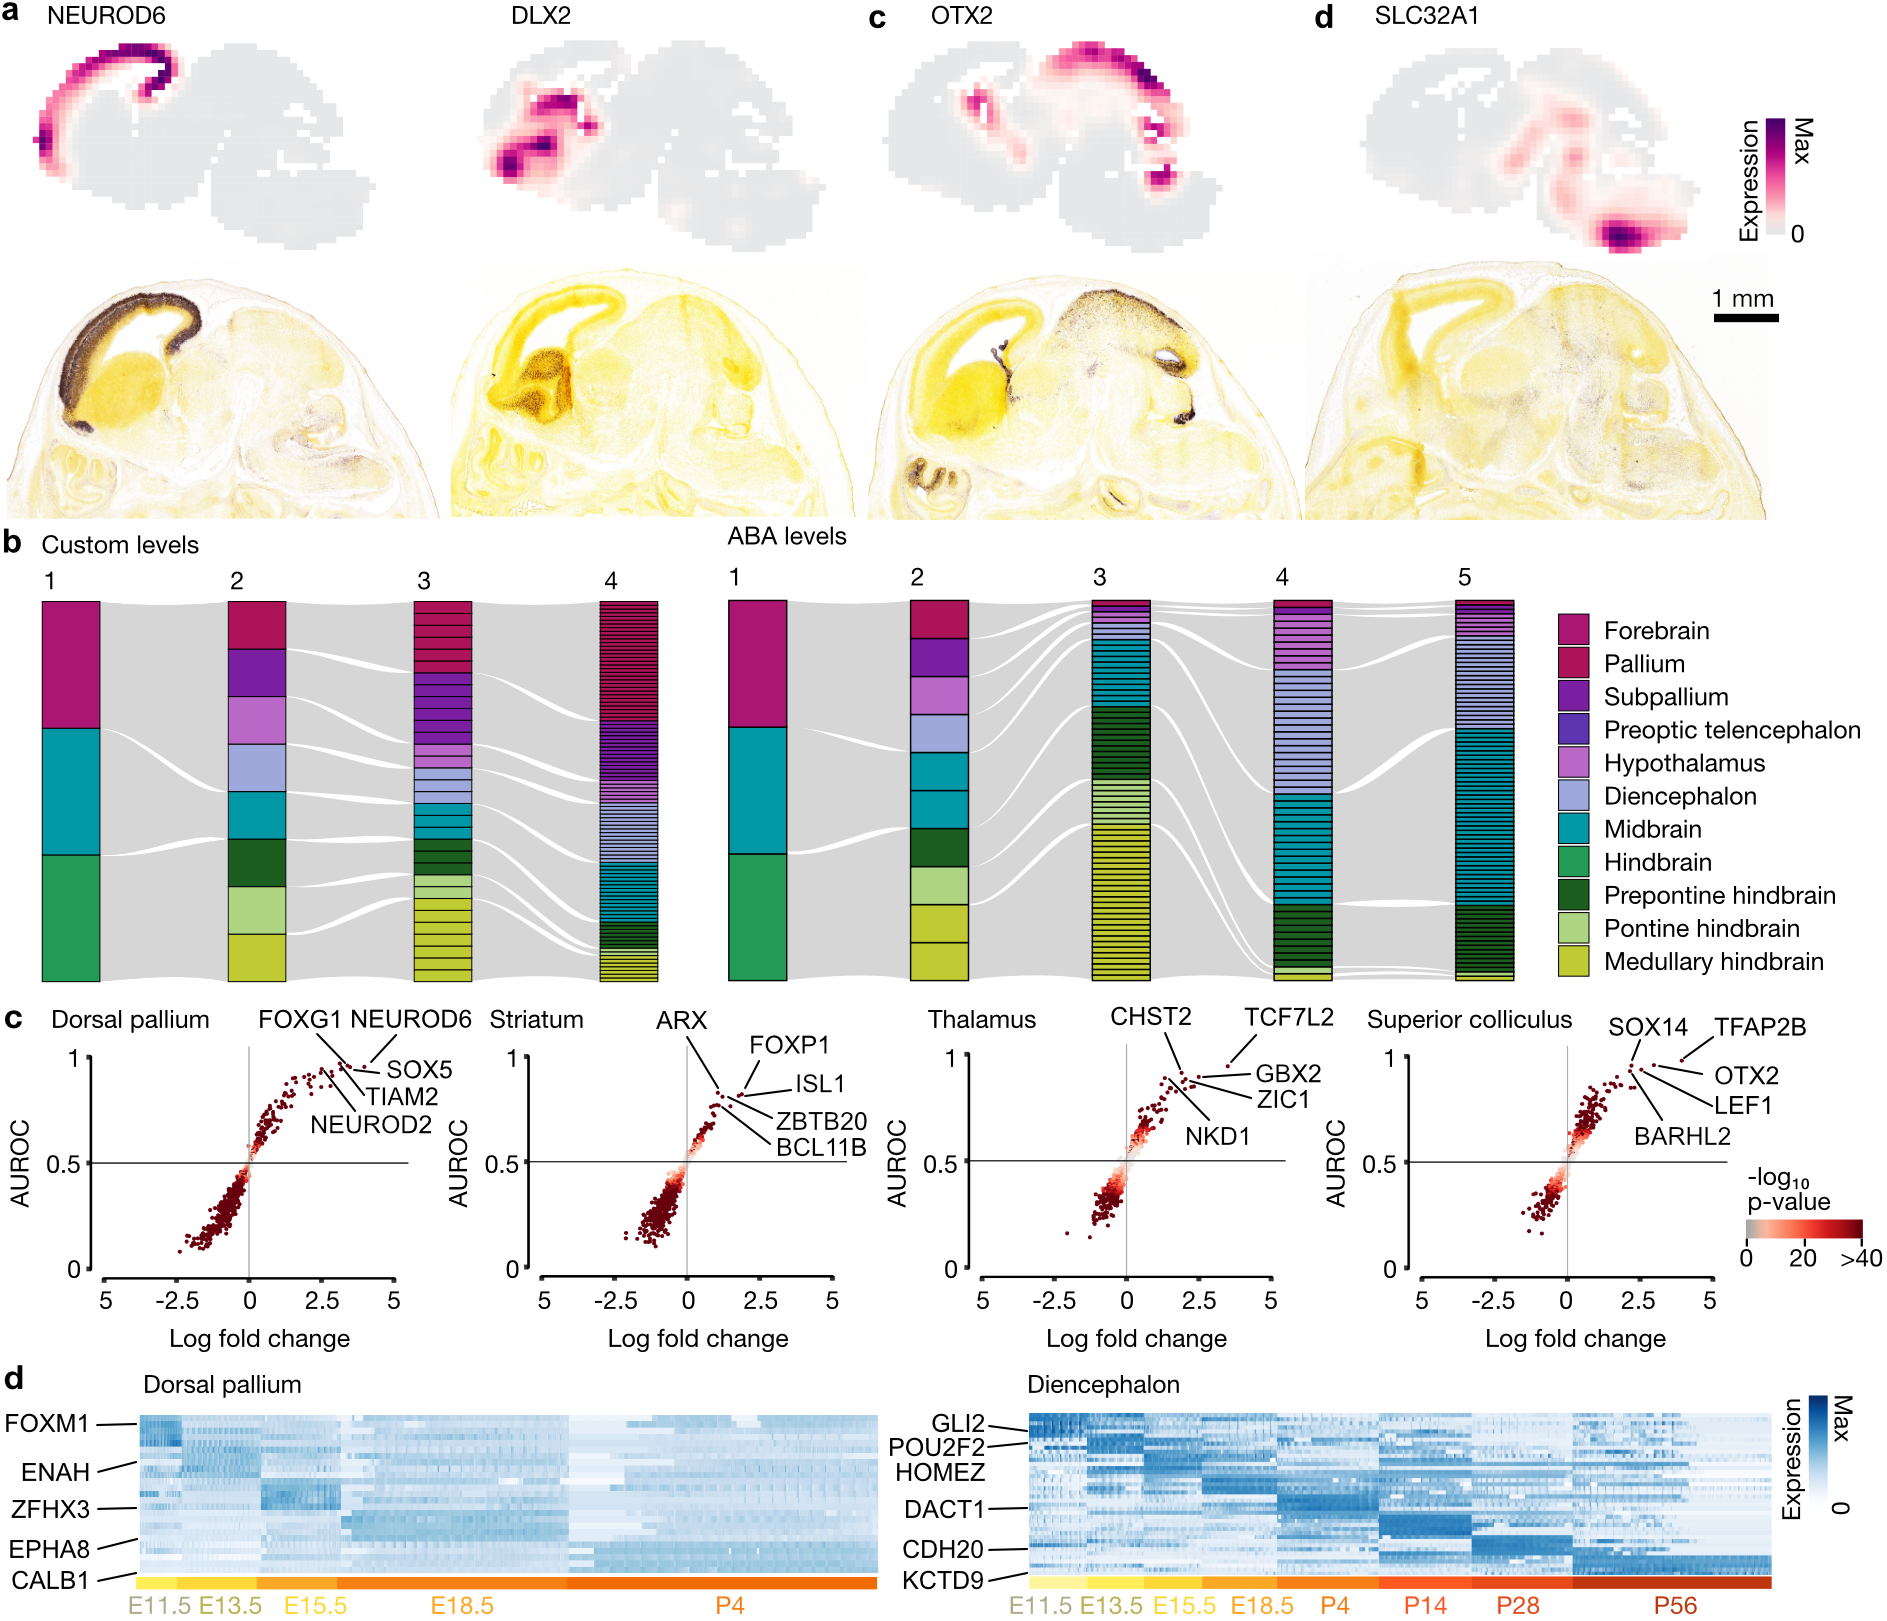
\includegraphics[width=\textwidth]{figures/voxhunt/Supp_1}
    \caption{\textbf{Supplemental characterization of voxel maps of developing mouse brain in situ hybridization data, related to Figure 2.2.} a) In silico expression maps compared to in situ hybridization patterns. Voxelized expression heatmaps (top) and in situ hybridization head images from the Allen Developing Mouse Brain Atlas (bottom) at E15.5 for NEUROD6, DLX2, OTX2, and SLC32A1. b) Hierarchical annotation levels of the developing mouse brain. Barcharts show how large structures are hierarchically subdivided into many smaller structures for custom annotation levels of similar size (left) in comparison to the first five annotation levels from the Allen Brain Atlas (right). Each box represents one annotated structure, colors represent custom level 1 on the first level and custom level 2 on all subsequent levels. c) Scatter plot showing feature selection for dorsal pallium, striatum, thalamus and superior colliculus. X-axis represents fold change and y-axis represents the area under the receiver operating characteristic curve (AUROC) metric for comparisons between the selected structure and all other brain structures. d) Heatmaps showing stage-specific genes for dorsal pallium and diencephalon binned by expression in the corresponding brain structure at different timepoints during development.}
    \label{fig:voxS1}
\end{figure}

\begin{figure}[h!]
    \centering
	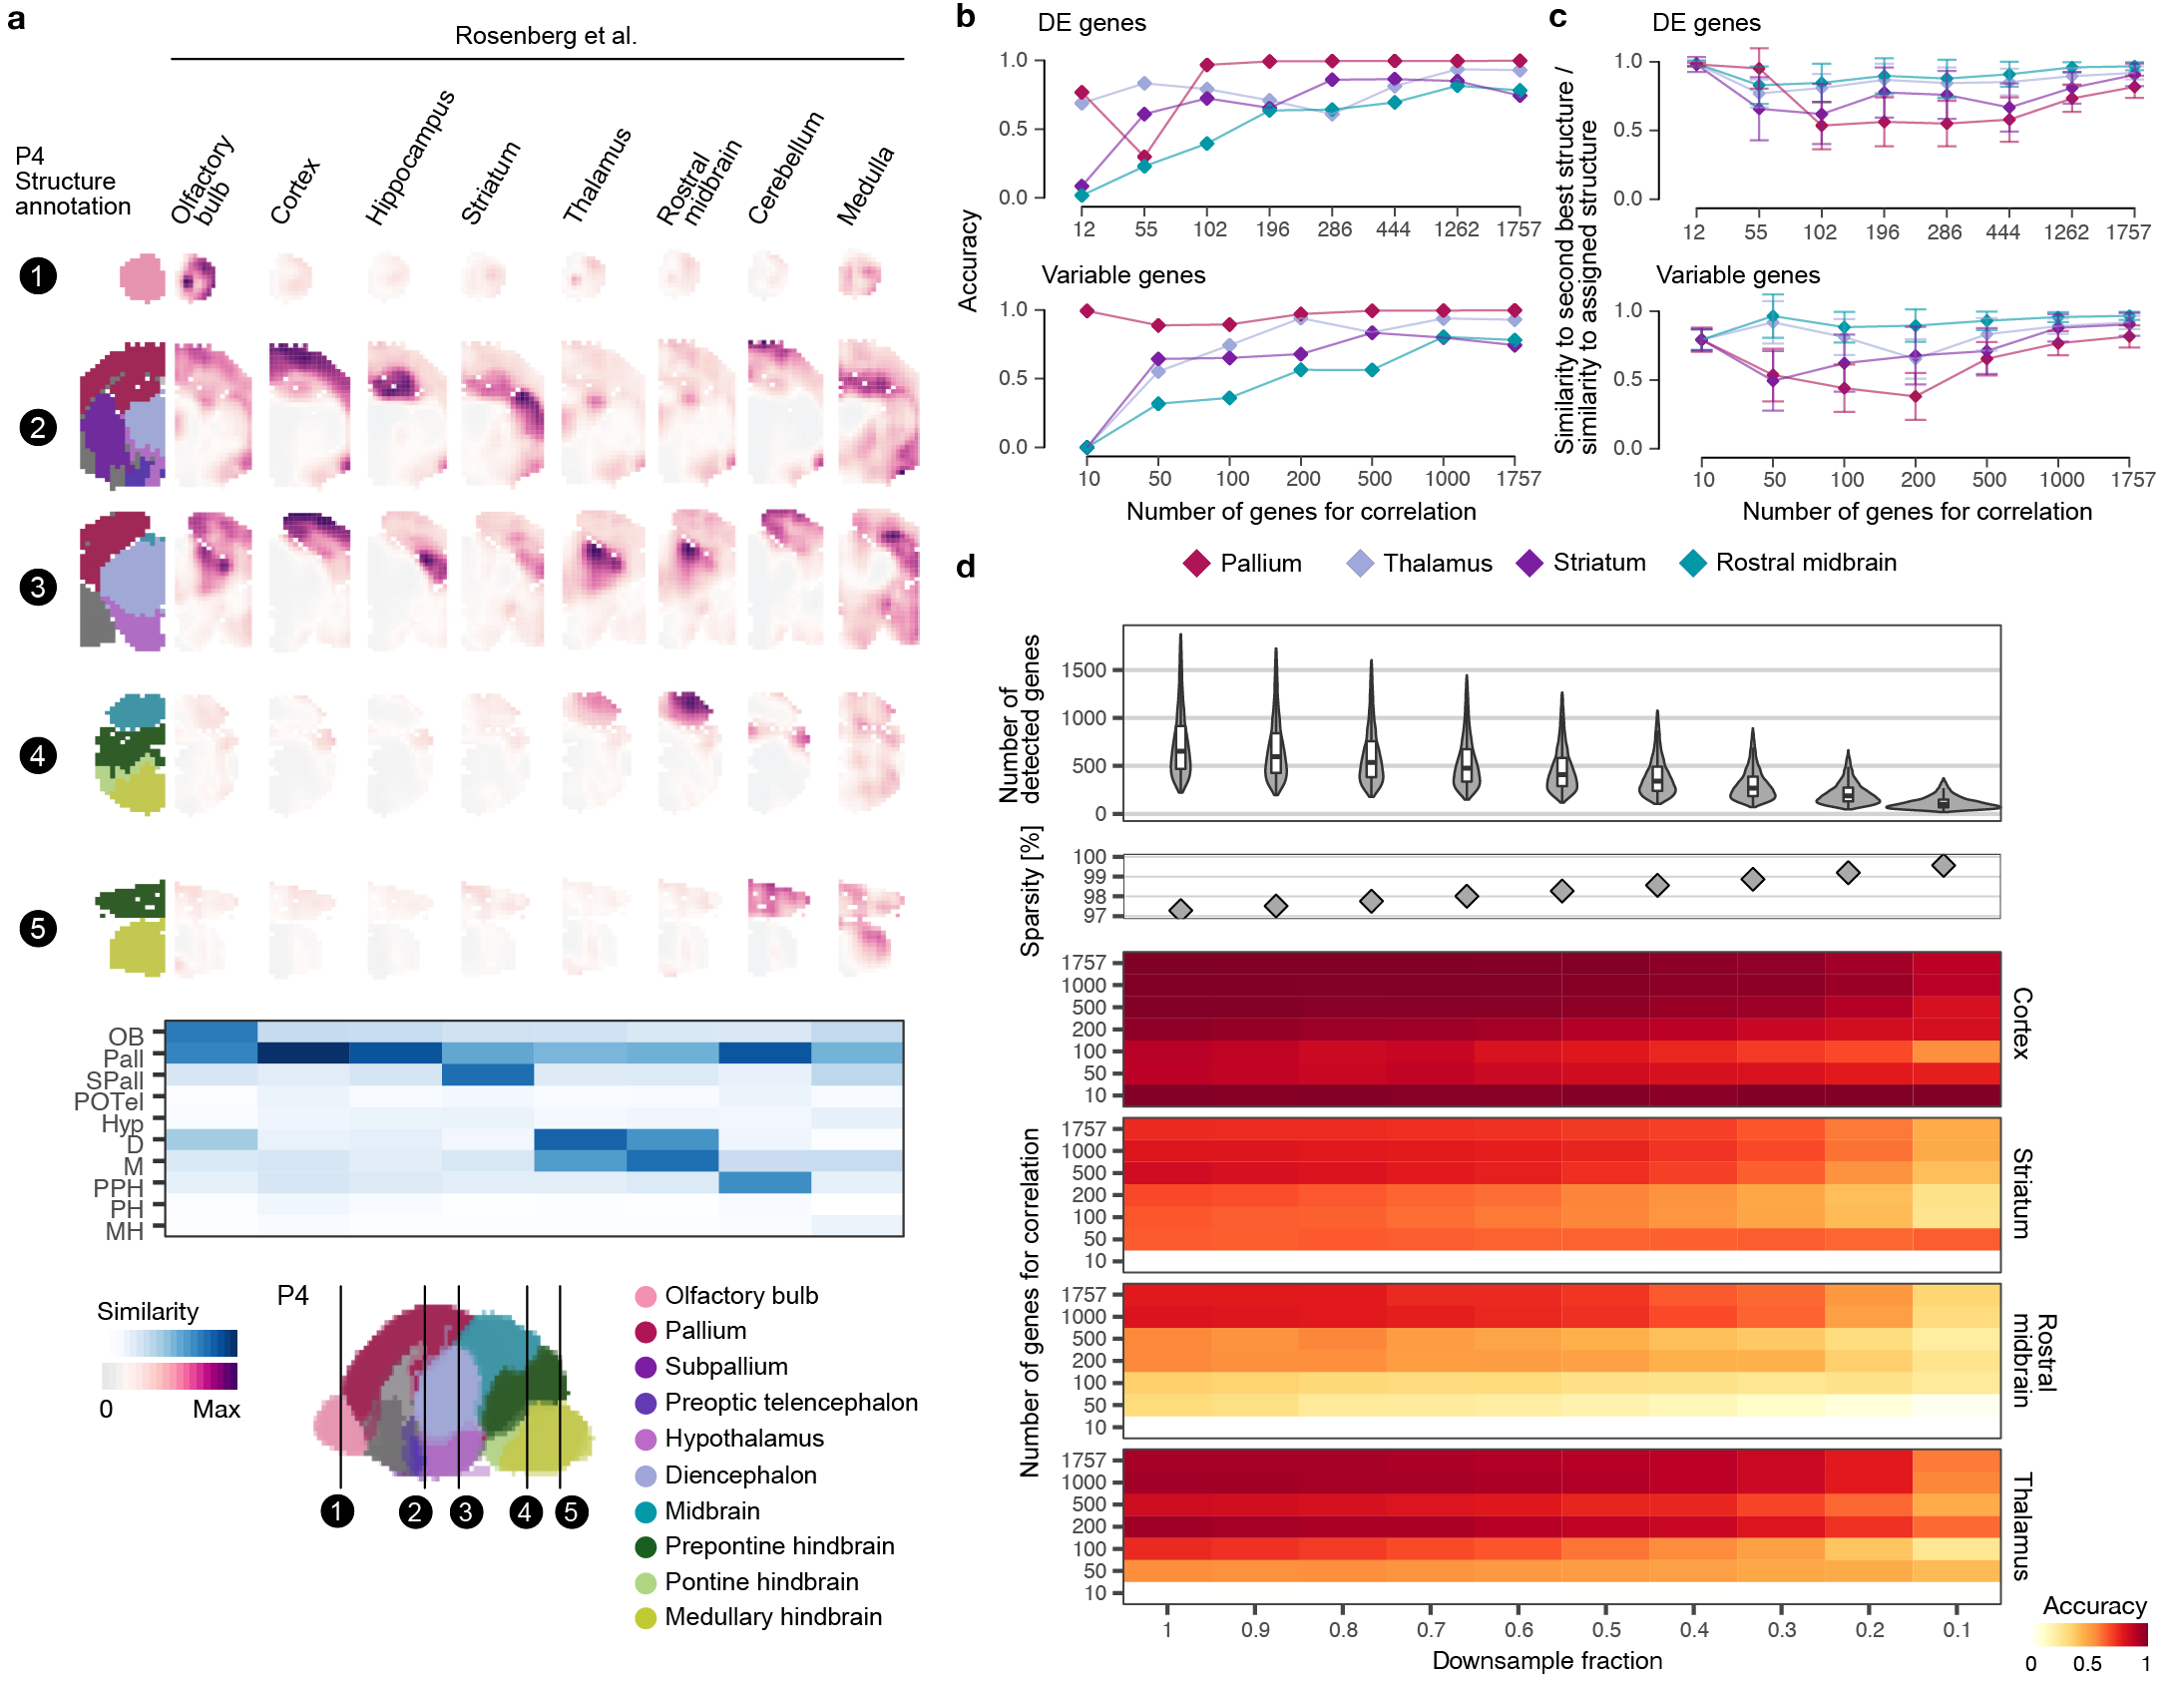
\includegraphics[width=\textwidth]{figures/voxhunt/Supp_2}
    \caption{\textbf{Effect of feature sets and data quality on spatial mapping, related to Figure 2.3.} a) Top: Coronal sections visualizing regional annotation and similarity of different neuronal populations from scRNA-seq of the P2 mouse brain (Rosenberg et al., 2018) to voxel maps of the P4 mouse brain. Bottom: Heatmap visualizing the mean similarity of these neuronal populations to brain structures at custom annotation level 2. b-d) Neuronal populations from scRNA-seq of the P2 mouse brain (Rosenberg et al., 2018) were used to assess accuracy and contrast of the spatial mapping to the P4 mouse brain under different conditions. b) Accuracy of maximum-similarity structure assignments using different numbers of features and feature selection criteria. We either considered the top differentially expressed genes between brain structures (top) or the most variable features (bottom). c) Contrast of spatial brain maps as determined by the ratio of correlation between the two most similar brain structures. Low values indicate high contrast. d) Stability of structure assignments to lower data quality assessed through downsampling of UMI counts. Top: Boxplots showing the number of detected genes per cell for different downsampling fractions. Middle: Fraction of zero entries in the expression matrix for different downsampling fractions. Bottom: Heatmaps showing the accuracy of structure assignments of four neuronal cell populations for different downsampling fractions and feature sets.}
    \label{fig:voxS2}
\end{figure}

\begin{figure}[h!]
    \centering
	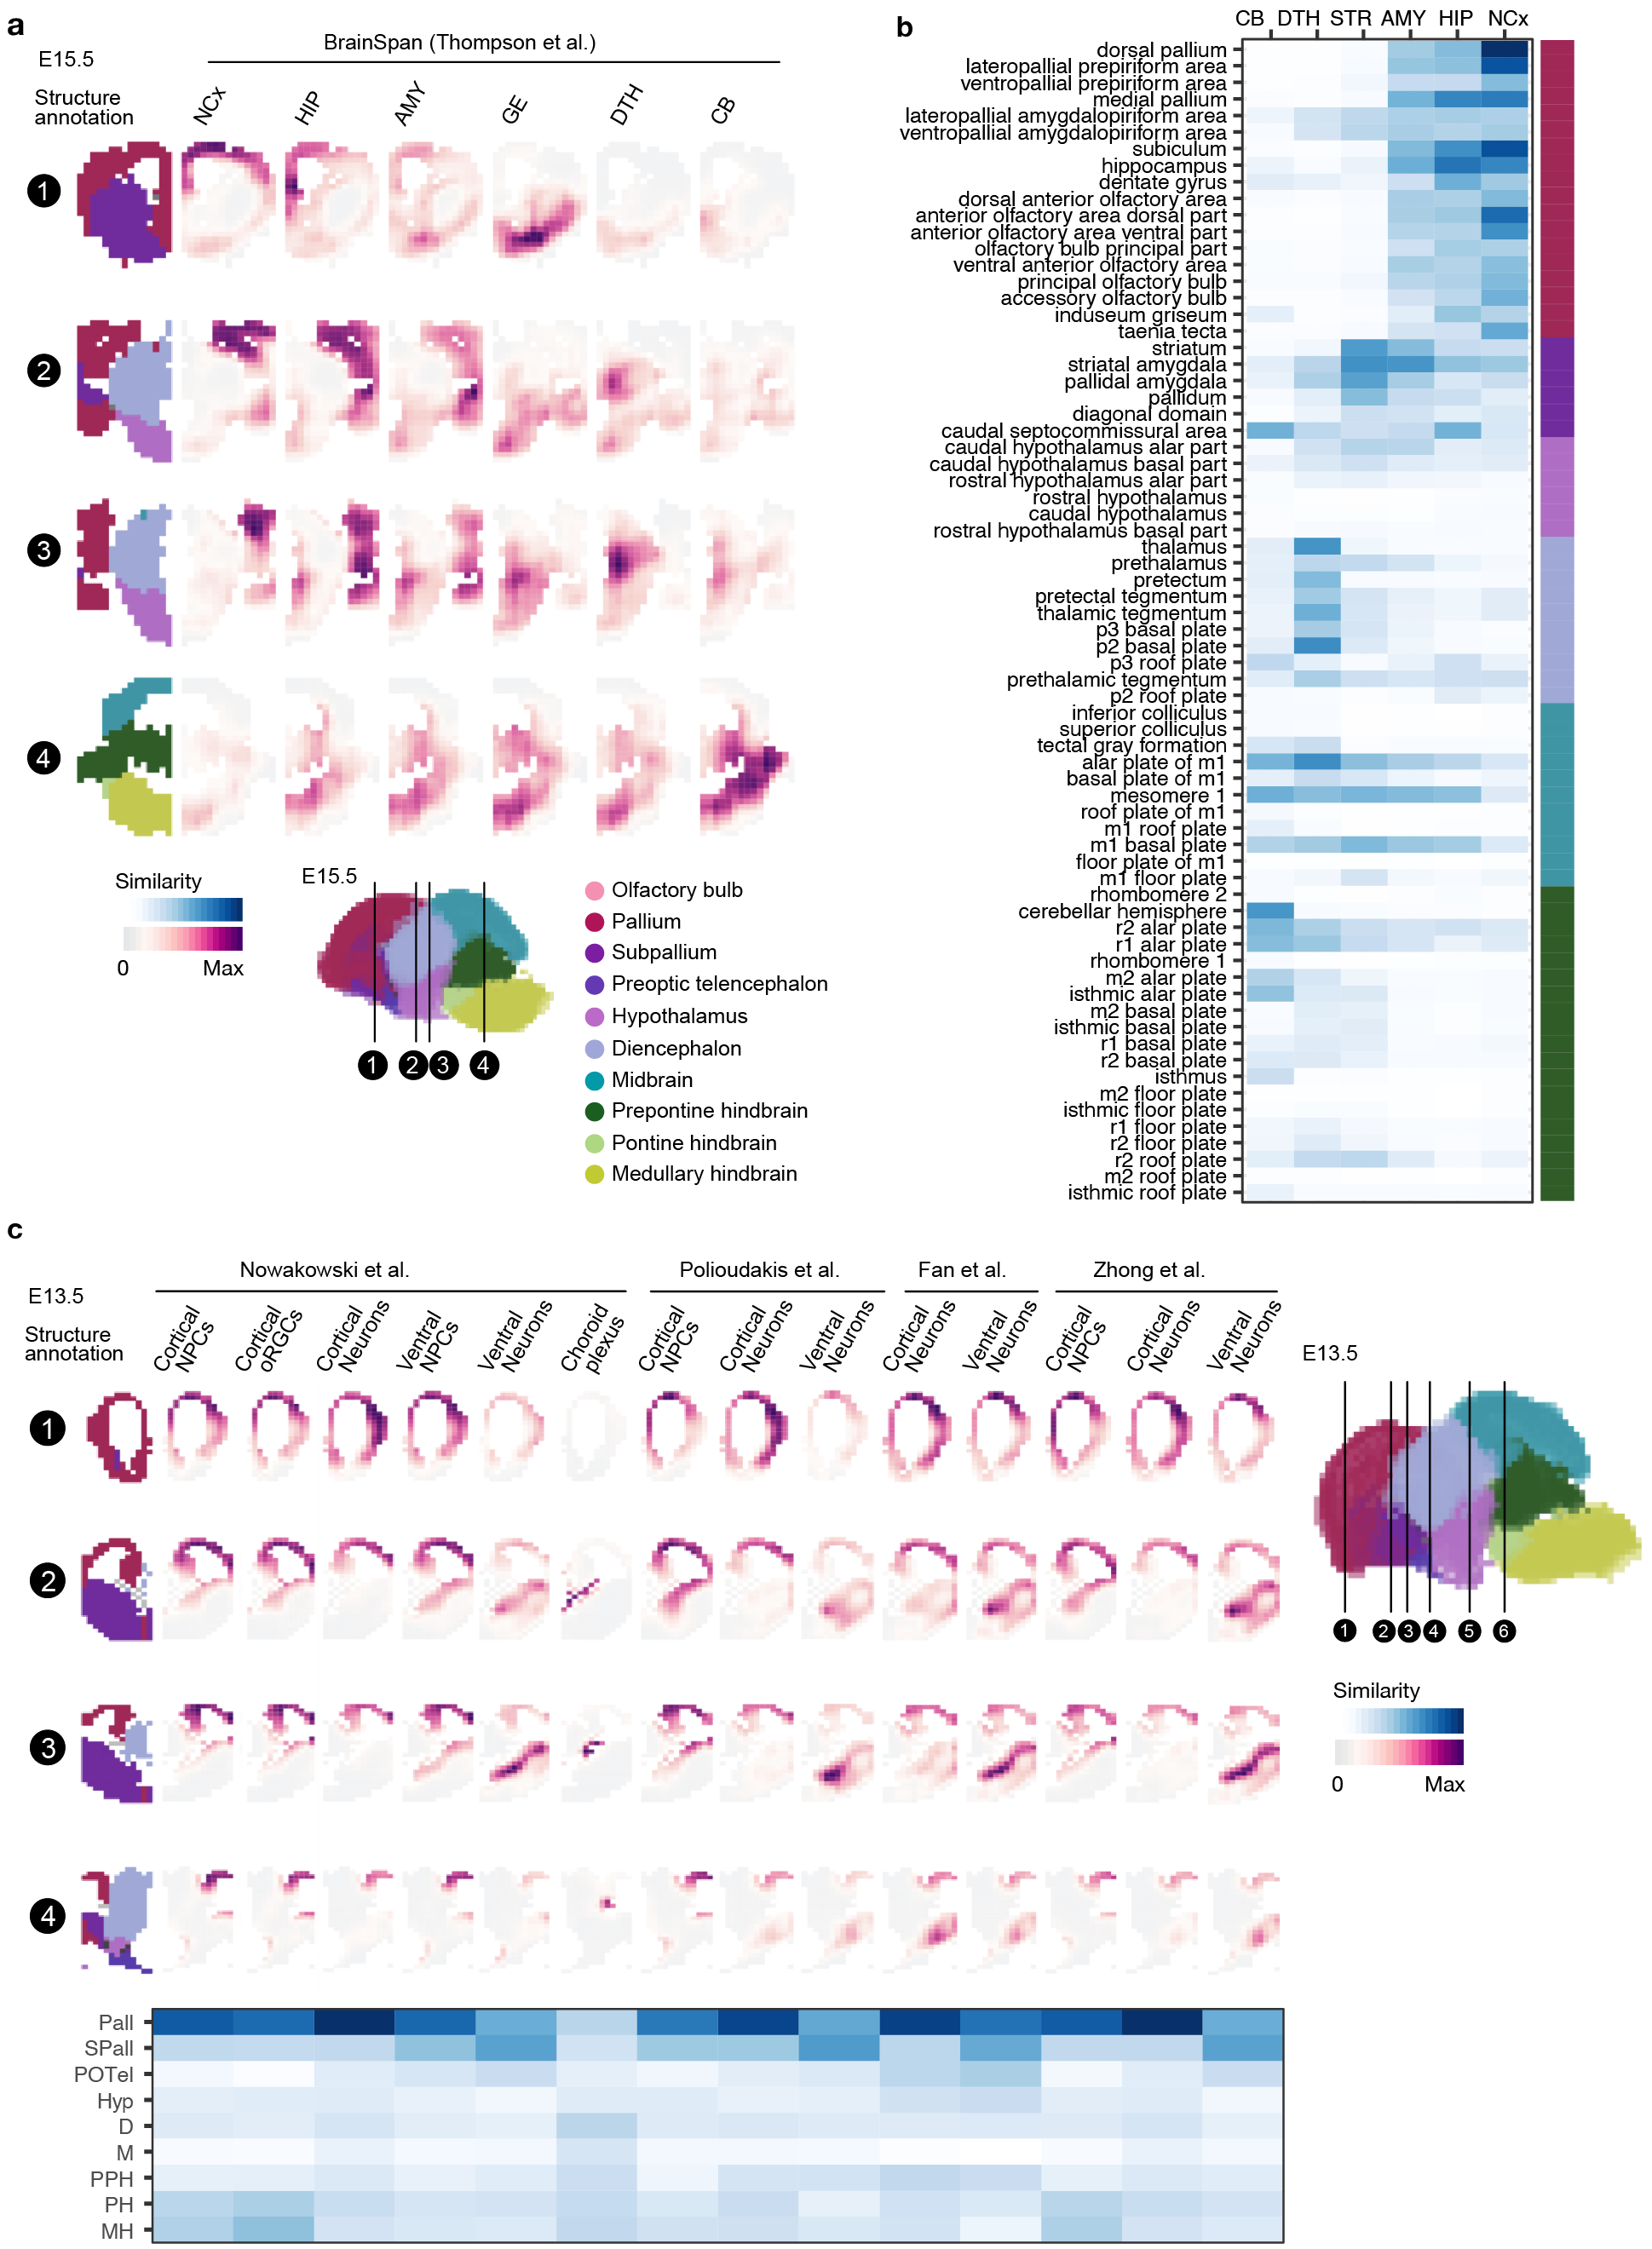
\includegraphics[width=\textwidth]{figures/voxhunt/Supp_3}
    \label{fig:voxS3}
\end{figure}

\begin{figure}[t!]
    \centering
    \caption{\textbf{Spatial similarity maps of brain regions and neuronal cells from primary human tissues, related to Figure 2.3.} a) Coronal sections visualizing regional annotation and scaled similarity scores of bulk RNA-seq data from microdissected human brain structures (wpc12 - wpc20) from BrainSpan to voxel maps of the E15.5 mouse brain. b) Heatmap showing similarity of microdissected human brain structures to E13.5 mouse brain structures at custom annotation level 4. c) Top: Coronal sections visualizing regional annotation and scaled similarity scores of human neuronal cell types from different studies to voxel maps of the E13.5 mouse brain. Bottom: Heatmap visualizing the mean similarity of neuronal cell populations to structures in the E13.5 mouse brain. NCx: neocortex, HIP: hippocampus, AMY: amygdala, GE: ganglionic eminence, DTH: dorsal thalamus, CB: cerebellum. NPC: Neural progenitor cell, oRGs: outer radial glia cells.}
\end{figure}


\begin{figure}[h!]
    \centering
	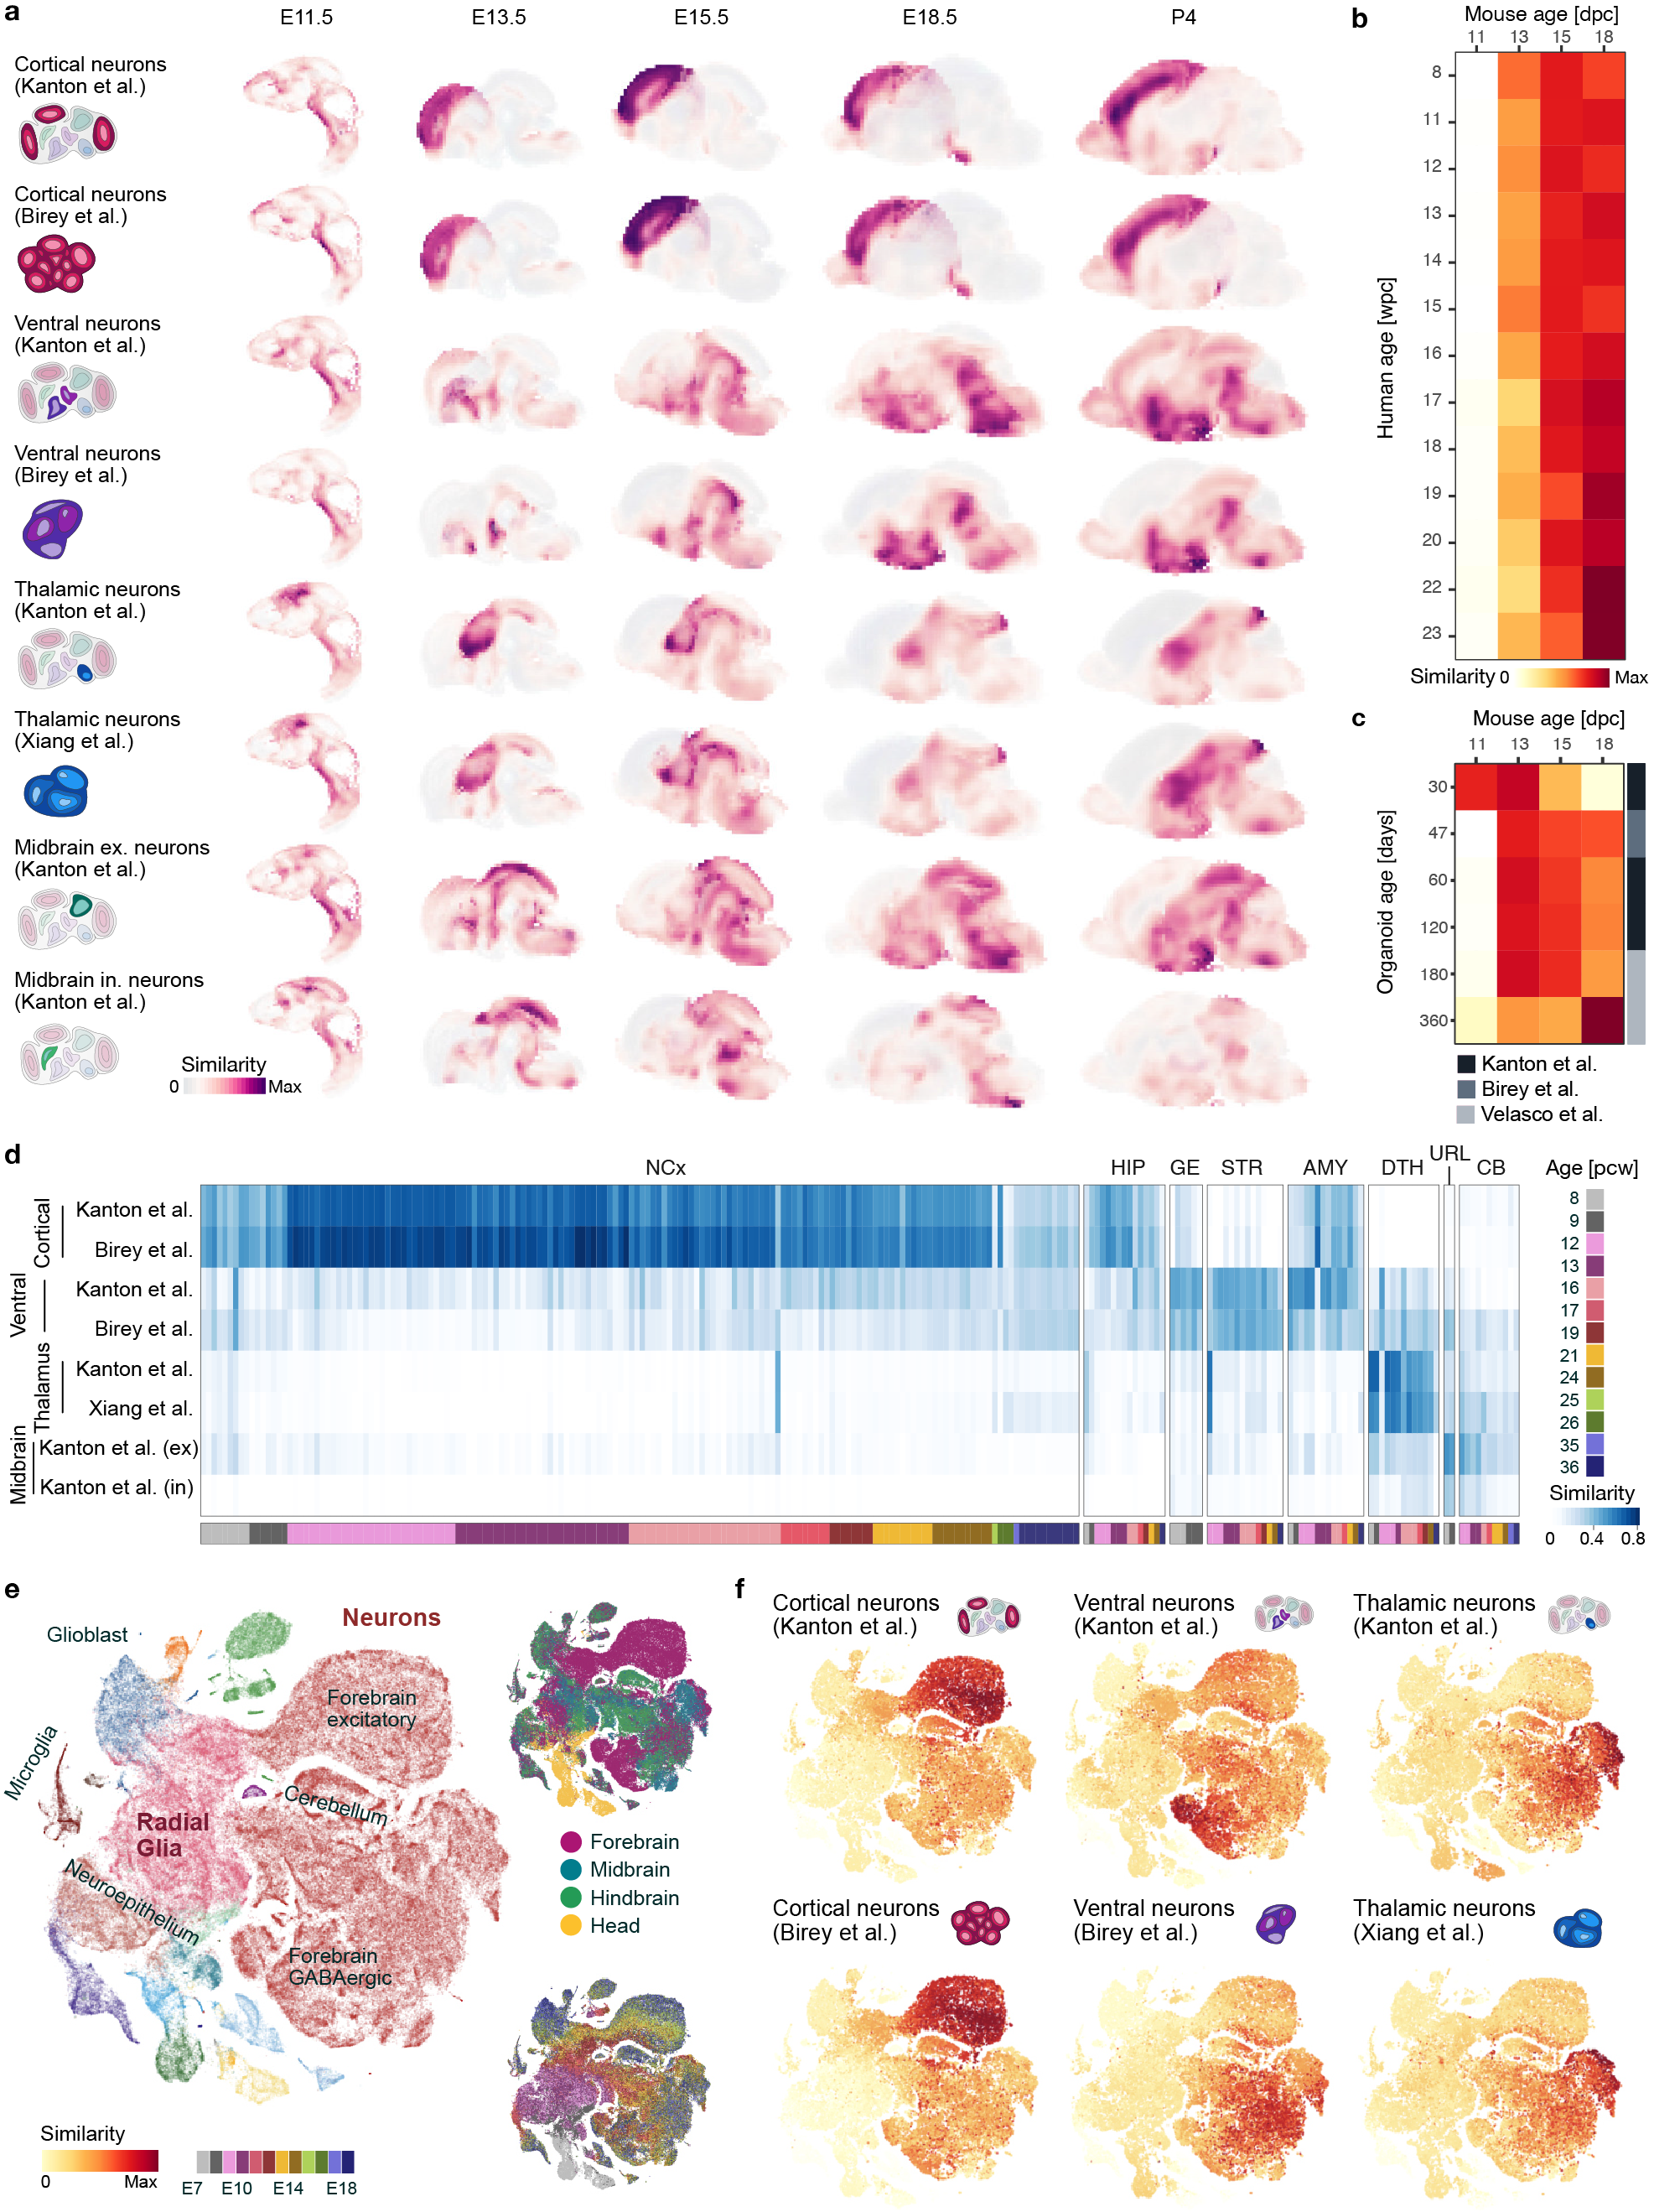
\includegraphics[width=\textwidth]{figures/voxhunt/Supp_4}
    \label{fig:voxS4}
\end{figure}

\begin{figure}[h!]
    \centering
    \caption{\textbf{Comparing brain organoid cell populations to reference brain maps, related to Figure 2.4.} a) Sagittal projections colored by scaled similarity scores of different organoid clusters from each organoid dataset to voxel maps of the developing mouse brain in stages E11.5 - P4. b) Heatmap showing the similarity of cortical neurons across human fetal development to the developing mouse pallium 11 - 18 dpc. For each population of cortical neurons and mouse developmental stage, we computed the mean of maximum correlating voxels in the mouse pallium. c) Similarity of cortical neurons from organoids grown through three different protocols (Birey et al., 2017; Kanton et al., 2019; Velasco et al., 2019) at 30 - 360 days of age to the mouse pallium at 11 - 18 dpc. d) Heatmap showing the similarity of organoid cell populations to bulk transcriptomes of microdissected human brain structures from BrainSpan. e) Structure, cell type and age annotations for the developing mouse brain dataset. NPC: Neural progenitor cell, CBC: Cilia bearing cell, ChP: Choroid plexus, Pall: Pallium, Spall: Subpallium, PPH: Prepontine hindbrain, NCx: Neocortex, HIP: Hippocampus, GE: Ganglionic eminence, STR: Striatum, AMY: Amygdala, DTH: Dorsal thalamus, URL: Upper rhombic lip, CB: Cerebellum. f) Scaled similarity scores of organoid cell populations to single cell transcriptomic data of the developing mouse brain (La Manno et al., 2020).}
\end{figure}

\begin{figure}[h!]
    \centering
	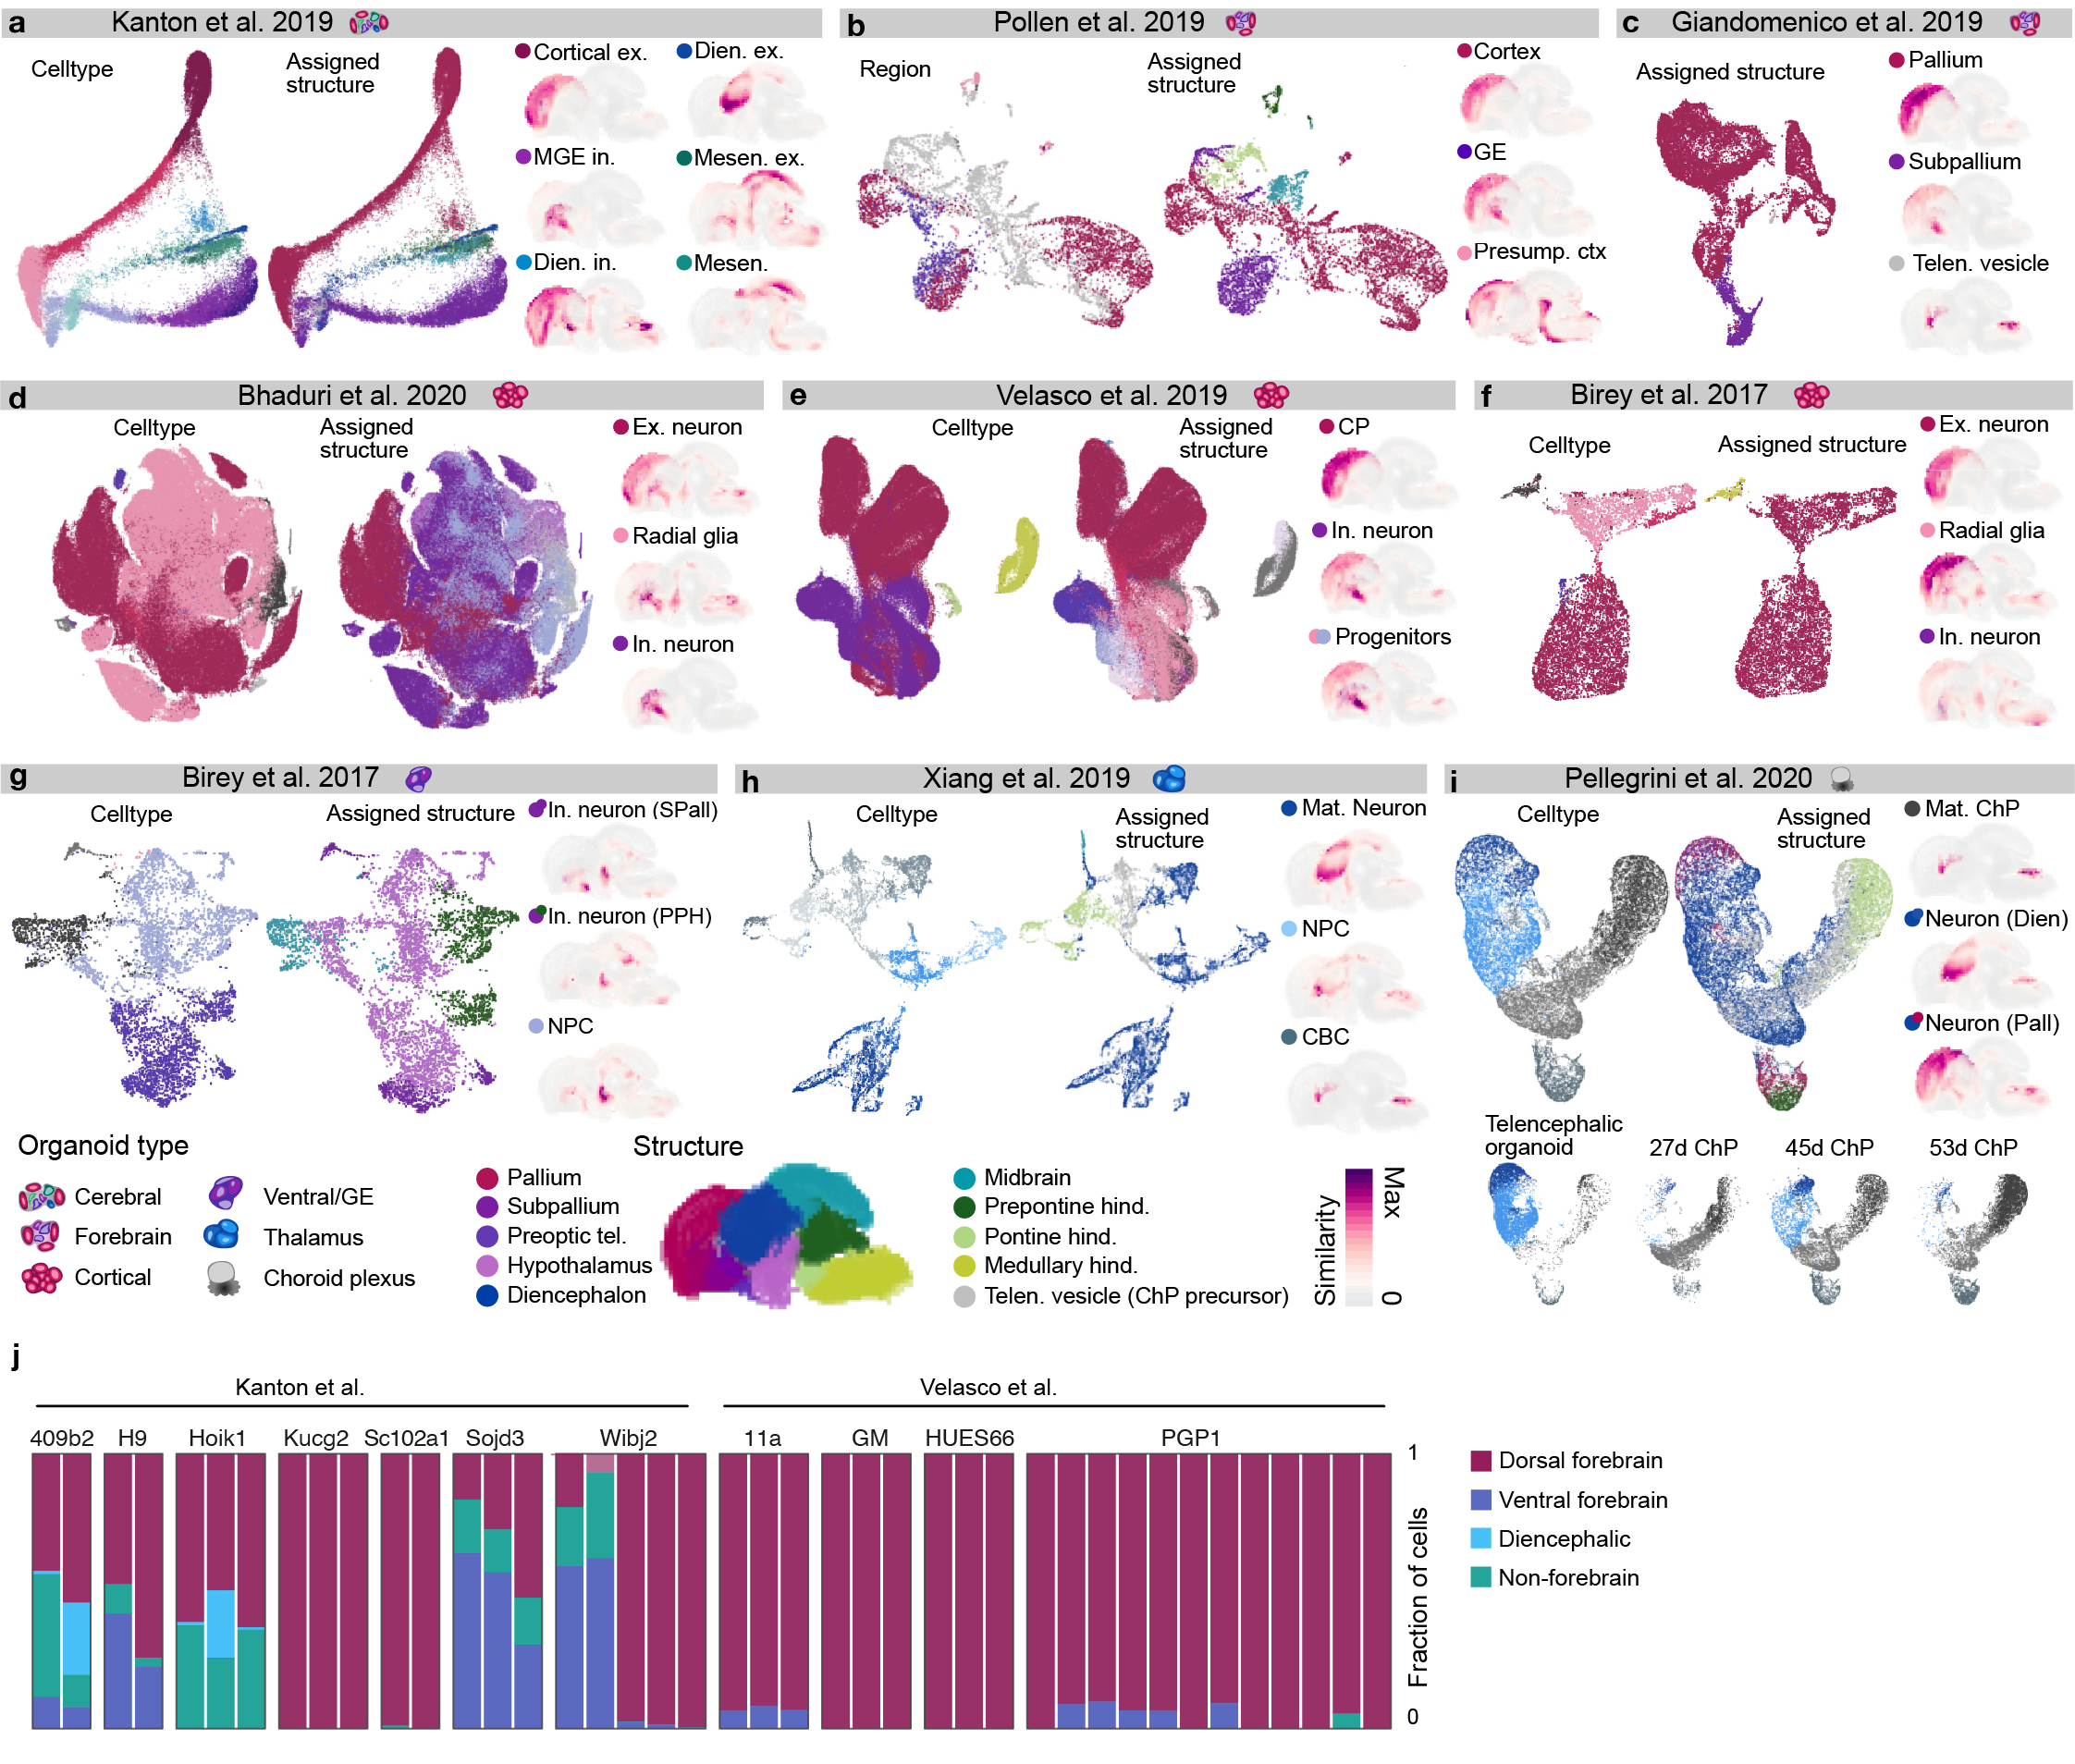
\includegraphics[width=\textwidth]{figures/voxhunt/Supp_5}
    \caption{\textbf{Comparing cell populations from different organoid protocols to spatial brain maps, related to Figure 2.4.} a-i) Brain region identities of organoid cell types from various published datasets. Cells are plotted using the embedding coordinates from the original publication (where available) or a custom UMAP embedding. For each dataset, the left panel shows cells colored by region or cell type where annotations were publicly available. The middle panel shows the clusters of cells colored by the brain structure containing the most highly correlated voxel of the average cluster transcriptome. The right panel shows sagittal sections visualizing scaled similarity scores of organoid cell populations to voxel transcriptomes. j) Comparison of organoids from different stem cell lines and batches with regard to their composition of neuron populations as annotated by VoxHunt. Each stacked bar plot represents scRNA-seq data from a single organoid.}
    \label{fig:voxS5}
\end{figure}

\begin{figure}[h!]
    \centering
	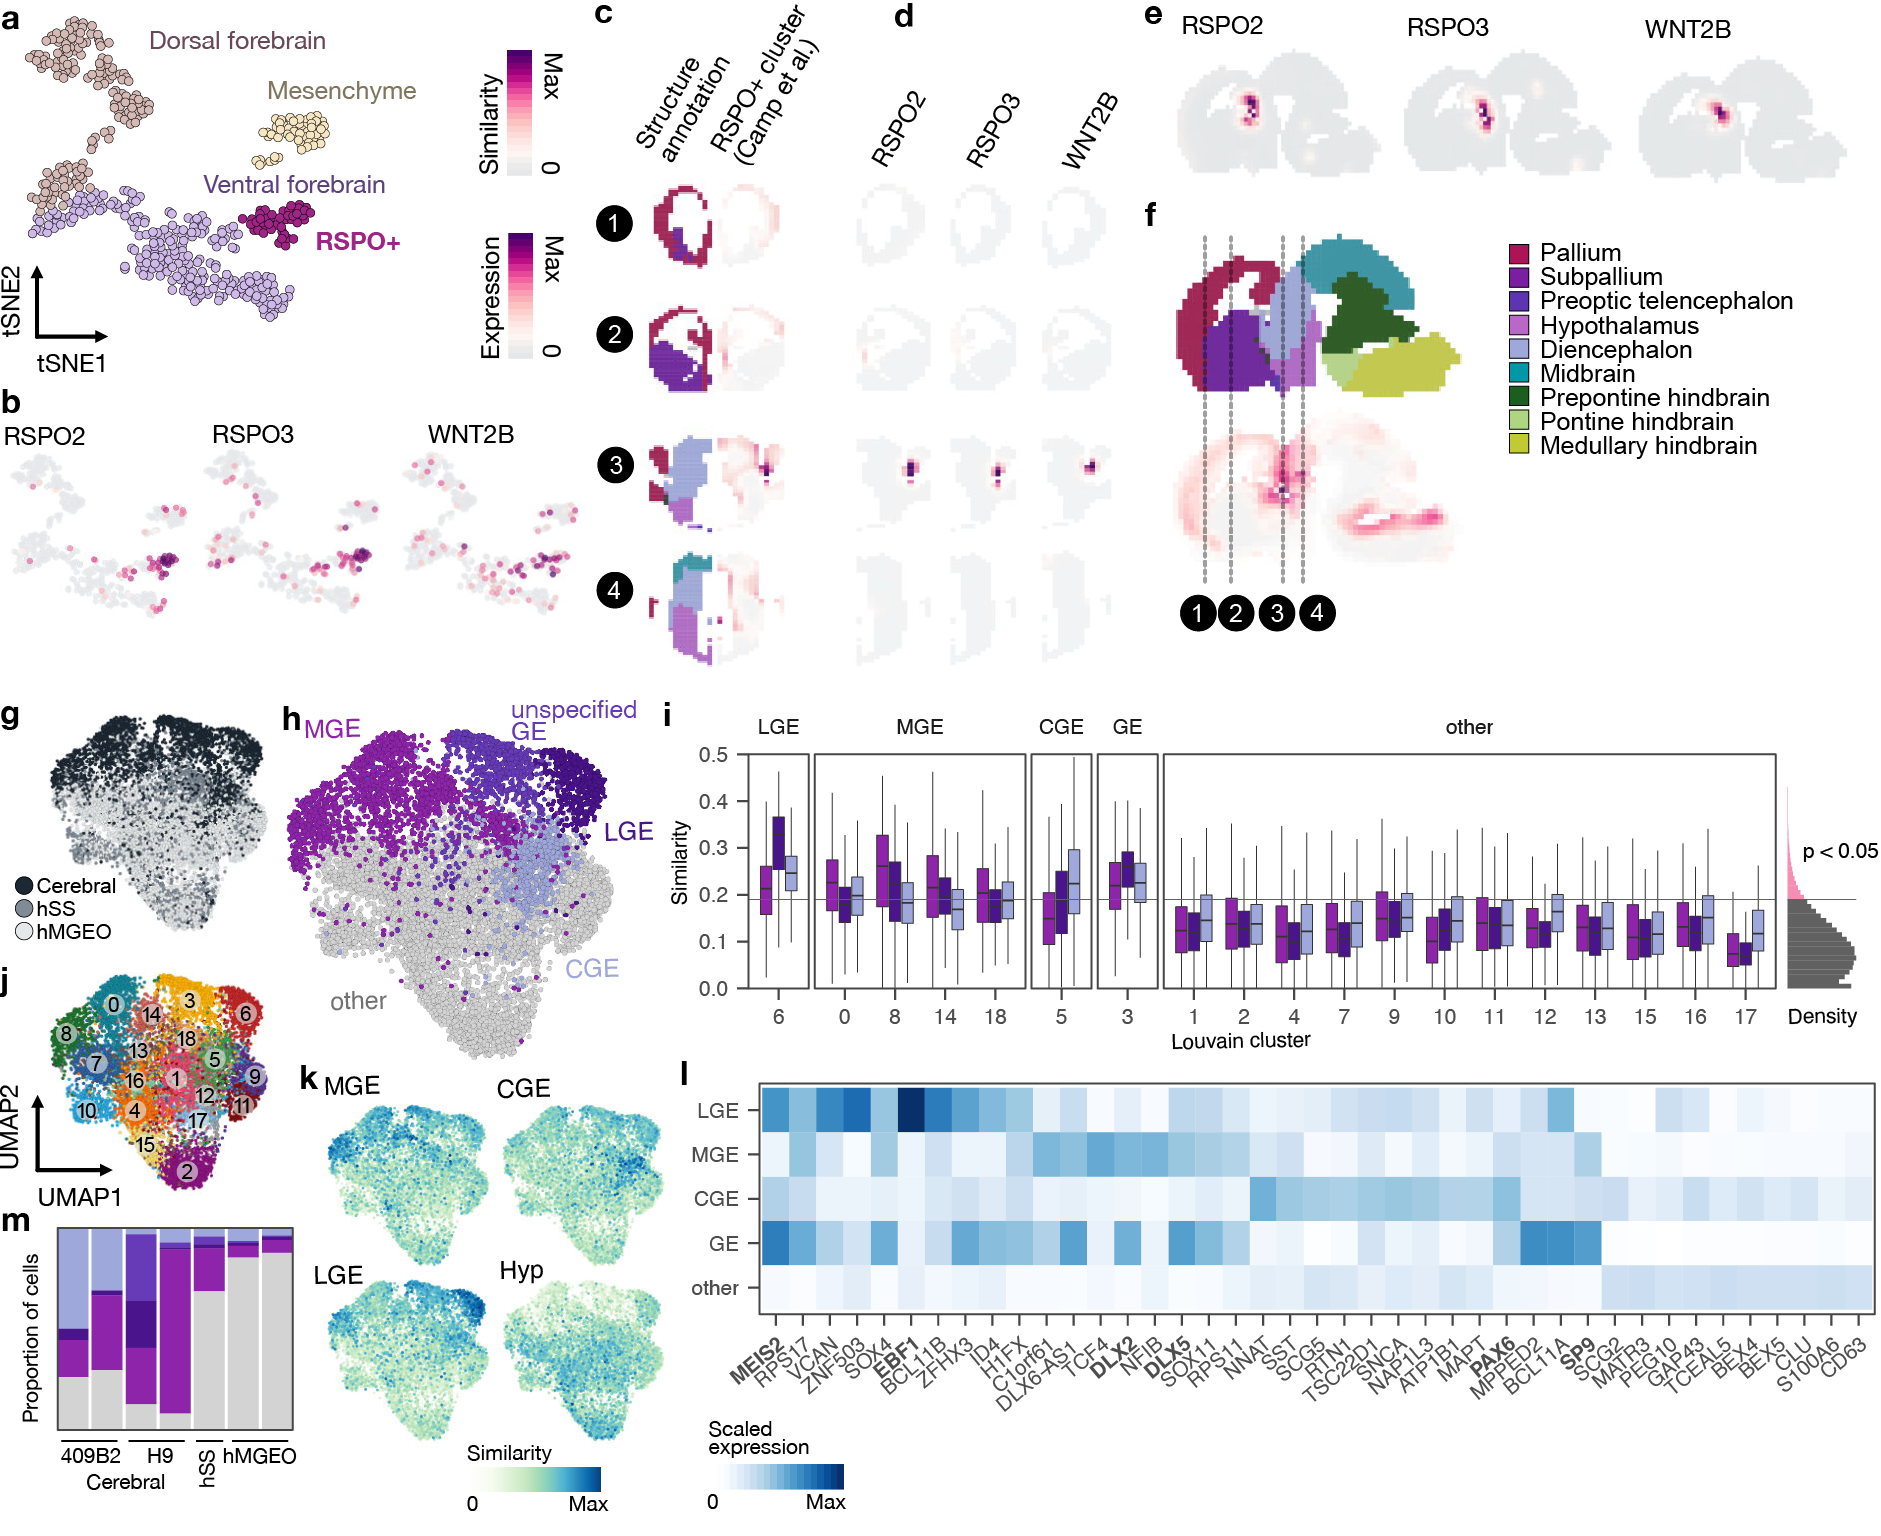
\includegraphics[width=\textwidth]{figures/voxhunt/Supp_6}
    \caption{\textbf{Spatial similarity maps resolve substructure identity of organoid cells, related to Figure 2.5.} a) tSNE embedding of single-cell transcriptomes from cerebral organoid cells based on the SMART-SEQ protocol implemented using Fluidigm C1 (Camp et al., 2015).  The previously unknown ‘RSPO+’ cluster is highlighted in purple. b) tSNE embedding colored by expression of genes marking the ‘RSPO+’ cluster. c) Coronal sections (6, 11, 22, 26) visualizing structure annotation and scaled similarity scores to voxel transcriptomes. d-e) Expression patterns of genes marking the ‘RSPO+’ cluster as maximum intensity projections across coronal sections 6, 11, 22 and 26 (d) and sagittal sections 2-5 (e). f) Top: Structure annotation of sagittal sections 2-5 of the E13.5 mouse brain. Bottom: Sagittal projections colored by scaled similarity scores of the ‘RSPO+’ cluster to voxel maps of the E13.5 mouse brain. g-h) A UMAP embedding of the integrated neuronal populations of ventral organoid datasets colored by g) protocol, h) assigned structure identity j) louvain cluster and k) scaled similarity to LGE, CGE, MGE and hypothalamus (Hyp). i) Similarity of louvain clusters to GE substructures LGE, MGE and CGE and distribution of similarity values across all cells. l) Heatmap showing the expression of top marker genes for each neuron population. Canonical GE marker genes are highlighted in bold. m) Neuron composition of individual organoids derived from different protocols (cerebral, hSS and hMGEO) and cell lines (409B2 and H9).}
    \label{fig:voxS6}
\end{figure}

\begin{figure}[h!]
    \centering
	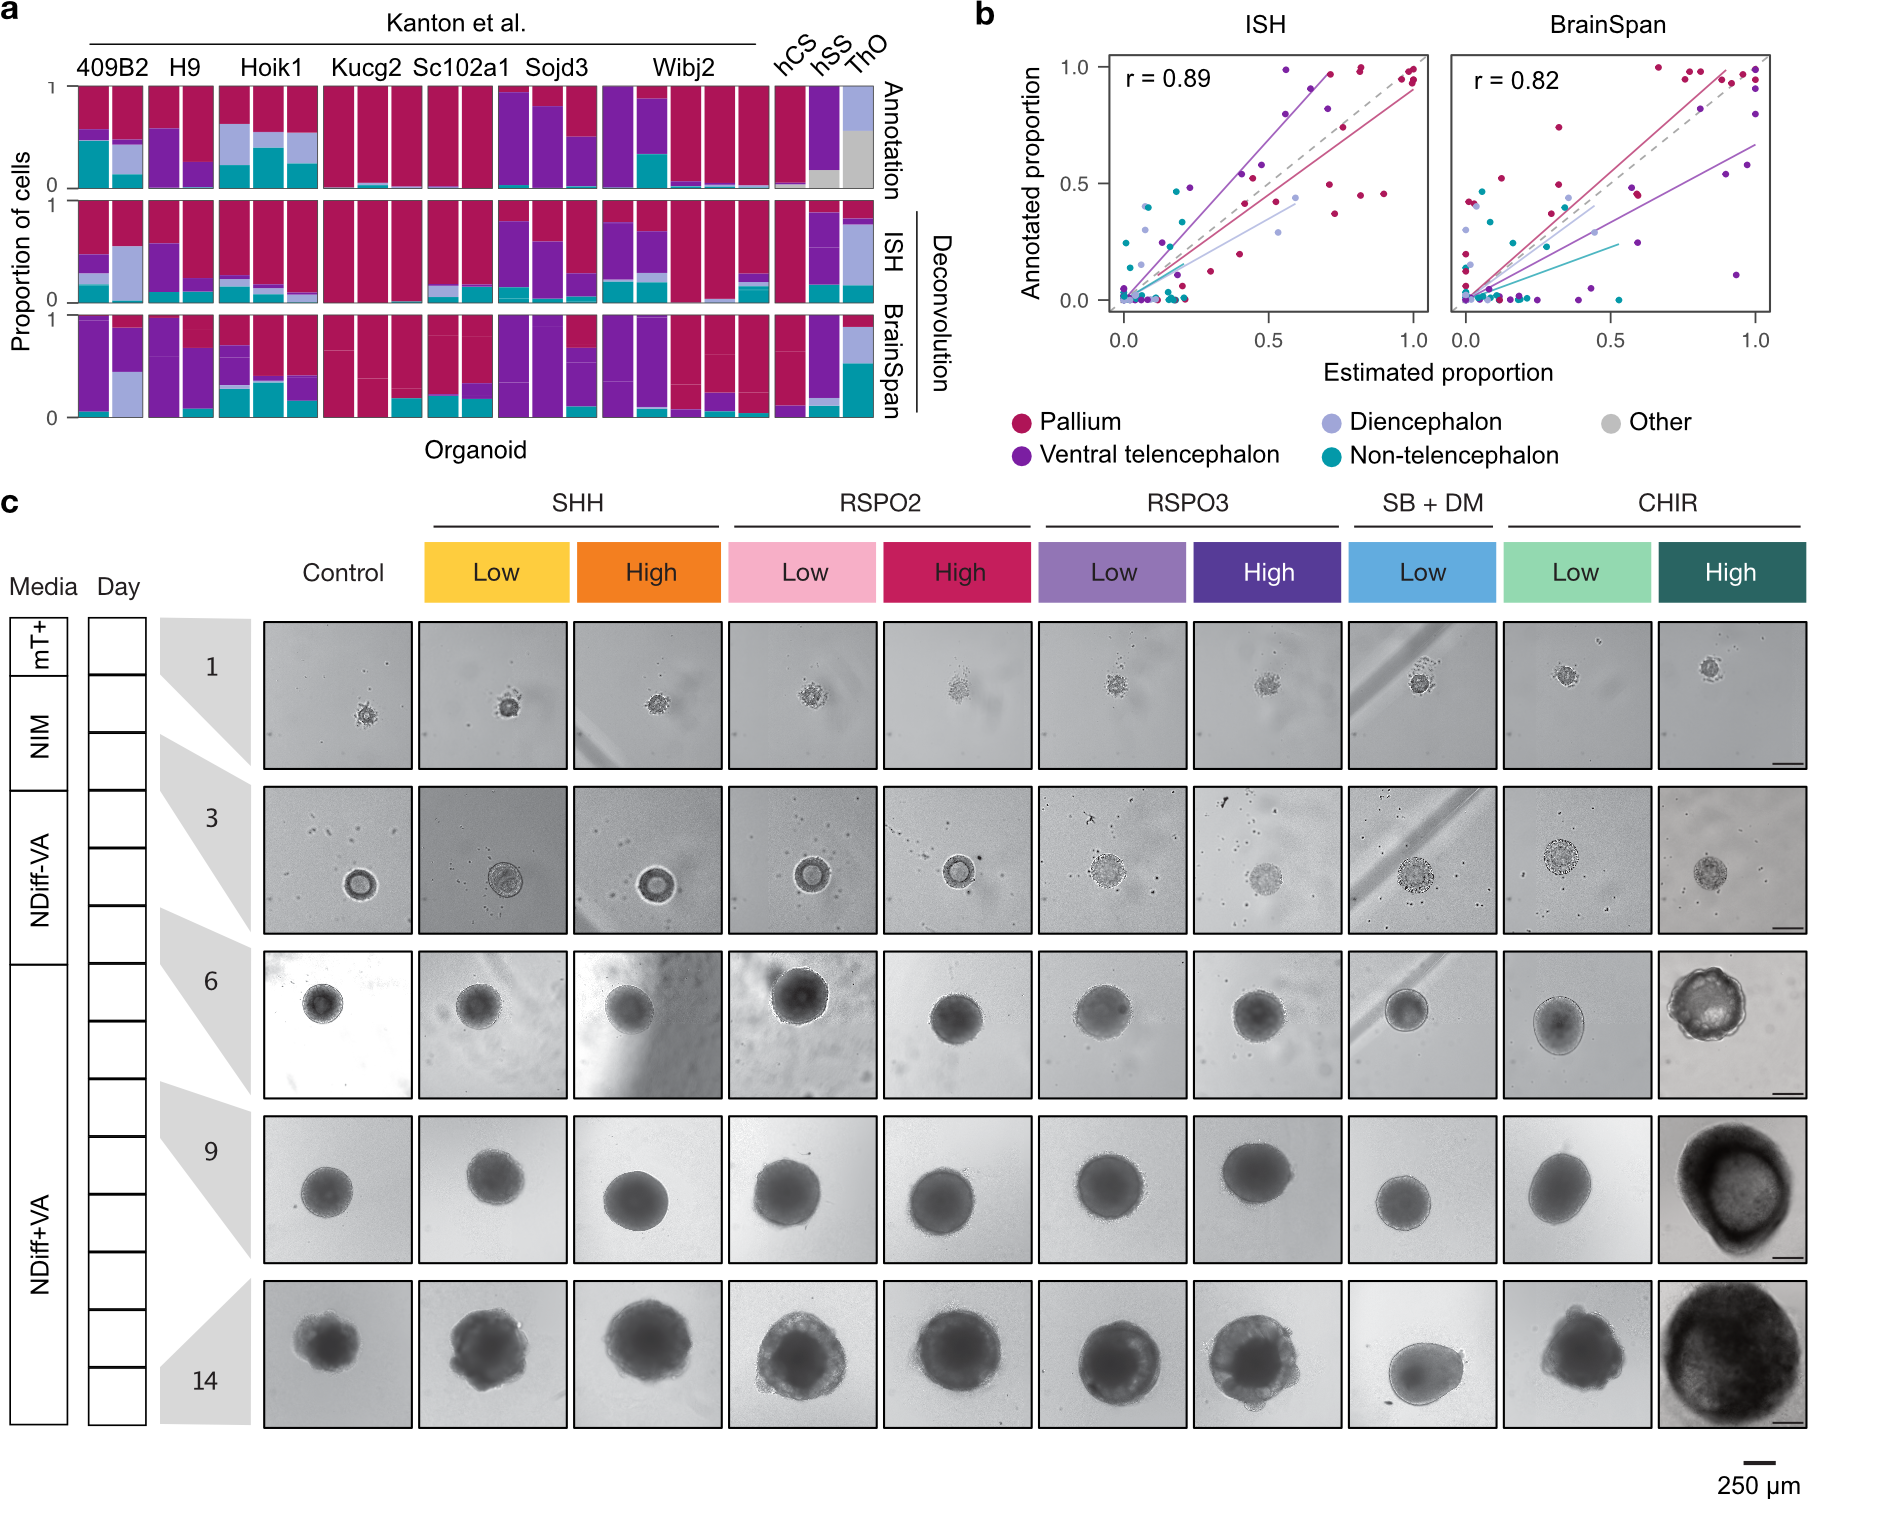
\includegraphics[width=\textwidth]{figures/voxhunt/Supp_7}
    \caption{\textbf{Deconvolution of organoid pseudo-bulk RNA-seq data and images of developing organoids from patterning screen, related to Figure 2.7.} a-b) Single-cell transcriptomics data from different organoid protocols, including cerebral (Kanton et al., 2019), cortical (hCS, (Birey et al., 2017)), ventral (hSS, (Birey et al., 2017)) and thalamic (ThO, (Xiang et al., 2019)) was summarized to pseudo-bulk and deconvoluted using either the Developing Mouse Brain Atlas (ISH) or Brainspan as a reference. a) Proportion of cells in organoids resembling different brain structures as assessed through single-cell transcriptome-based annotations (Annotated) or through deconvolution of pseudo-bulk transcriptomes (Deconvolution). b) Correlation of annotated proportions and proportions estimated through deconvolution. c) Organoids were grown in separate wells of an ultra-low attachment 96-well plate and exposed to different morphogens in low and high doses from day 3 until day 6 of culture. Pictures were taken at regular time points during organoid development.}
    \label{fig:voxS7}
\end{figure}

\clearpage

\topparagraph{Supplementary Data}

\noindent
All supplementary data items can be obtained from polybox with the following link: \\ \href{https://polybox.ethz.ch/index.php/s/FQvxGTwZe6wqNcR}{https://polybox.ethz.ch/index.php/s/FQvxGTwZe6wqNcR} 

\vspace{0.5cm}
\noindent
{\normalfont\footnotesize\sffamily\textbf{Supplementary Videos 2.1-2.5 | Three-dimensional spatial similarity maps of organoid cell types.} Related to Figure 2.4.}

\vspace{0.25cm}
\noindent
{\normalfont\footnotesize\sffamily\textbf{Supplementary Table 2.1 | Feature sets used to compute spatial correlation maps.} Related to STAR Methods section ‘Spatial correlation maps of organoid cells transcriptome’.}





\clearpage

\newpage
\thispagestyle{empty}
\
\newpage
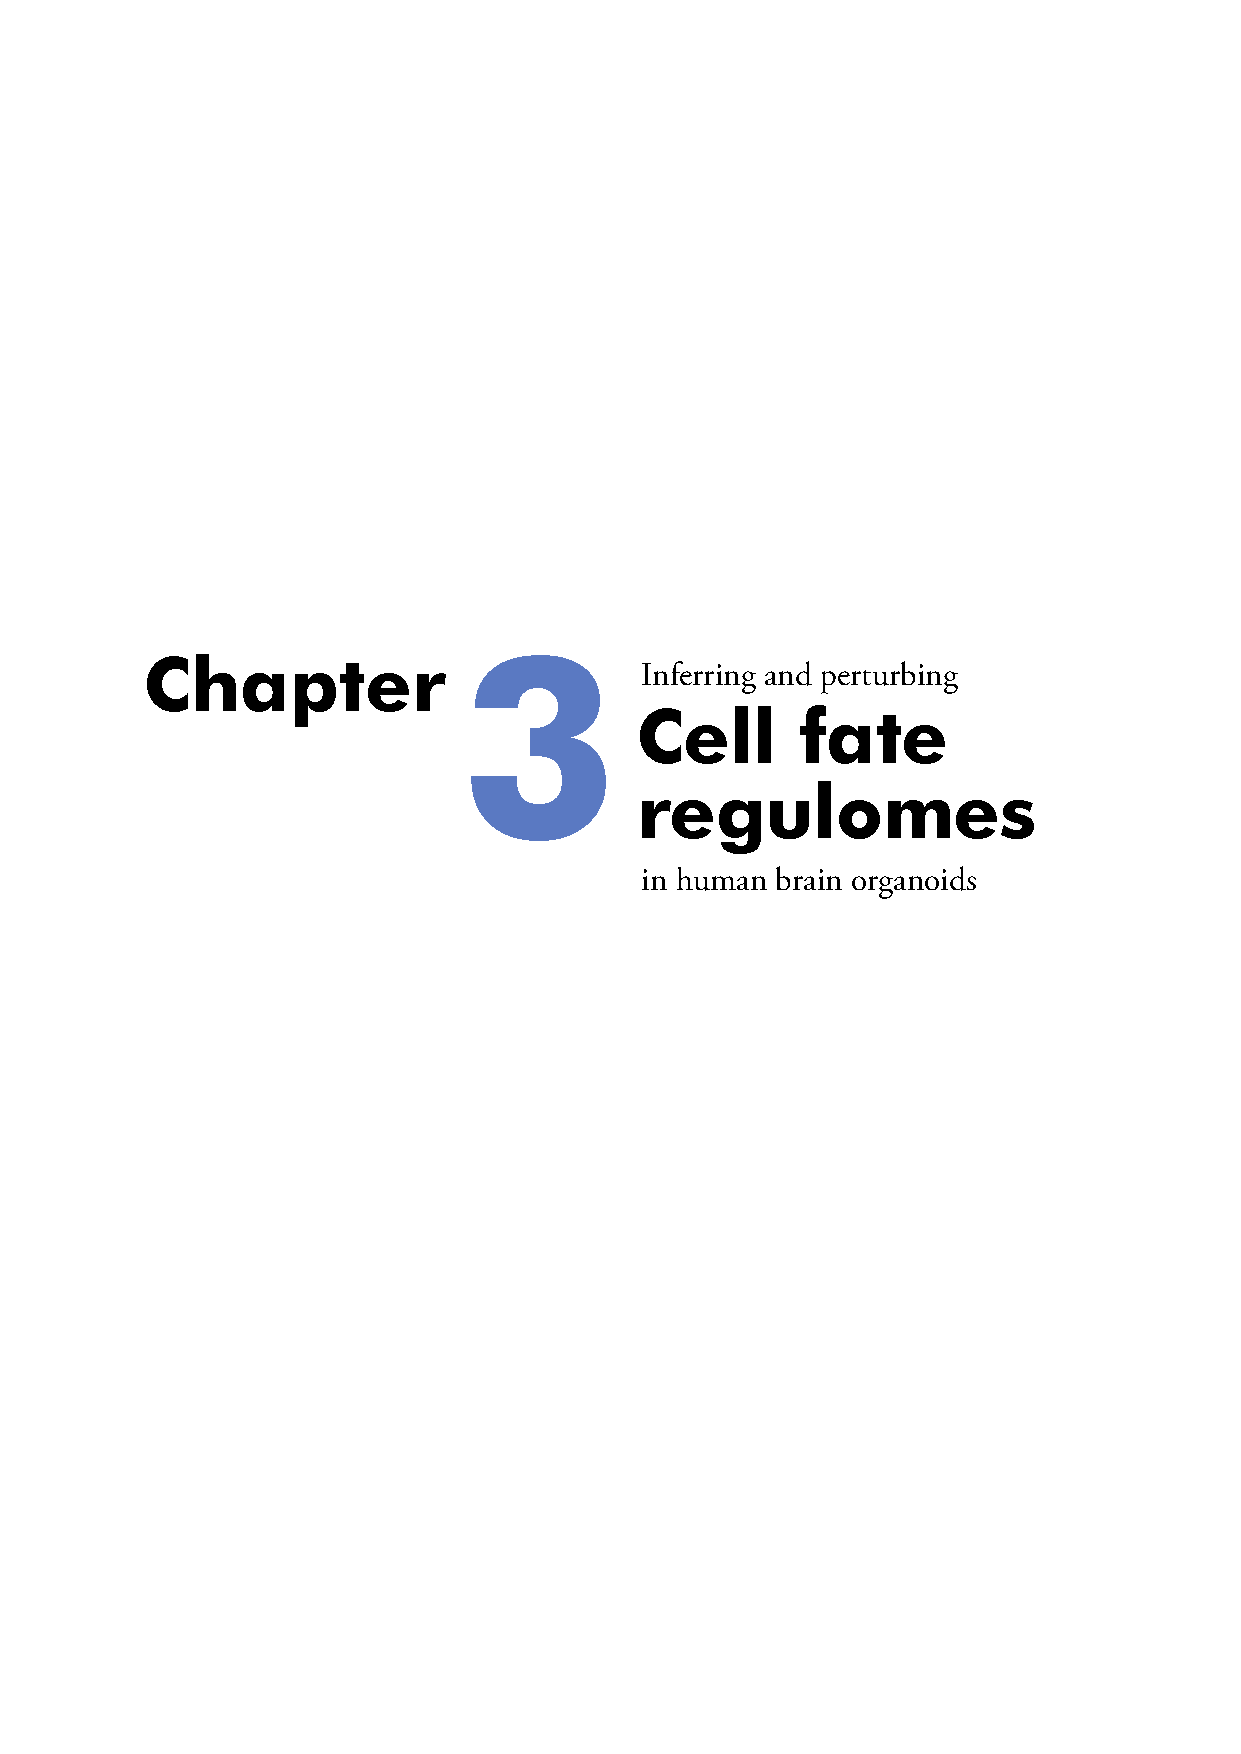
\includepdf[fitpaper=true, pages=-]{pdfs/chapter_3.pdf}

\thispagestyle{plain}
\section{Inferring and perturbing cell fate regulomes in human brain organoids}
\markboth{Inferring and perturbing cell fate regulomes in human brain organoids}{}


\vspace{0.5cm}

Chapter 3 is an adapted version of the article 'Inferring and perturbing cell fate regulomes in human brain organoids', which has been accepted for publication in \textit{Nature} in July 2022. I contributed the computational analyses of the presented single-cell RNA-seq and ATAC-seq data, the multiome data and data from perturbation experiments. I also contributed the development of the Pando R-package for gene regulatory network inference, as well as assistance with culturing organoids.

\vspace{1cm}

\noindent
{\large\textsc{Authors}}

\noindent
Jonas Simon Fleck\textsuperscript{1$*$}, 
Sophie Martina Johanna Jansen\textsuperscript{1$*$}, 
Damian Wollny\textsuperscript{2}, 
Fides Zenk\textsuperscript{1}, 
Makiko Seimiya\textsuperscript{1}, 
Akanksha Jain\textsuperscript{1}, 
Ryoko Okamoto\textsuperscript{1}, 
Malgorzata Santel\textsuperscript{1}, 
Zhisong He\textsuperscript{1\$}, 
J. Gray Camp\textsuperscript{3,4,5\$}, 
Barbara Treutlein\textsuperscript{1\$}

\vspace{0.5cm}

\noindent
$\ast$ Equal contribution\\
\$ Corresponding author

\vspace{1cm}

\noindent
{\large\textsc{Affiliations}}

\noindent
\textsuperscript{1} Department of Biosystems Science and Engineering, ETH Zürich, Basel, Switzerland\\
\textsuperscript{2} Max Planck Institute for Evolutionary Anthropology, Leipzig, Germany\\
\textsuperscript{3} Institute of Molecular and Clinical Ophthalmology, Basel, Switzerland\\
\textsuperscript{4} University of Basel, Basel, Switzerland\\
\textsuperscript{5} Current affiliation: Roche Institute for Translational Bioengineering (ITB), Roche Pharma Research and Early Development, Roche Innovation Center Basel, Switzerland

\vspace{1cm}

\noindent
{\large\textsc{Correspondence}} 

\noindent
Zhisong He (\href{mailto:zhisong.he@bsse.ethz.ch}{zhisong.he@bsse.ethz.ch})\\
J. Gray Camp (\href{mailto:grayson.camp@iob.ch}{grayson.camp@iob.ch})\\
Barbara Treutlein (\href{mailto:barbara.treutlein@bsse.ethz.ch}{barbara.treutlein@bsse.ethz.ch})

\vspace{1cm}

\noindent
\clearpage
{\large\textsc{Author contributions}} 

\noindent
S.J. generated organoids used in this study, with support from J.S.F., R.O. and D.W.. S.J. generated all single-cell transcriptome and accessible chromatin datasets with support from M.Sa.. S.J. performed the CROP-seq and the multiome experiments. J.S.F., D.W., M.Se. constructed CROP-seq vectors. S.J. generated the GLI3 iPSC lines and generated the scRNA-seq data on GLI3 KO organoids with help from D.W.. F.Z., S.J. performed western blots for GLI3. F.Z. performed the Cut\&Tag experiment. S.J., A.J. generated IHC and HCR data. J.S.F. performed the analysis of the scRNA-seq/scATAC-seq developmental time course with support from Z.H., S.J.. J.S.F. analyzed the multiome data of the neuroepithelial stage. J.S.F. developed the Pando R package. J.S.F. analyzed the CROP-seq data with support from Z.H.. S.J.. J.S.F. analyzed the GLI3 KO scRNA-seq and multiome data as well as the SHH perturbation multiome data. J.S.F., S.J., Z.H., J.G.C., B.T. designed the study and wrote the manuscript.

\vspace{1cm}

\noindent
{\large\textsc{Preprint link}} 

\noindent
\href{https://doi.org/10.1101/2021.08.24.457460}{https://doi.org/10.1101/2021.08.24.457460}



\subsection{Abstract}
Self-organizing and unguided neural organoids grown from pluripotent stem cells combined with single-cell genomic technologies provide opportunities to explore gene regulatory networks (GRNs) underlying human brain development. Here we acquire single-cell transcriptome and accessible chromatin data over a dense organoid time course covering neuroepithelial formation, patterning, brain regionalization, and neurogenesis, and identify temporally dynamic and brain region-specific regulatory regions. We develop Pando, a flexible framework that incorporates multi-omic data and transcription factor binding site predictions to infer a global GRN describing organoid development. We use pooled genetic perturbation with single-cell transcriptome readout to assess transcription factor requirement for cell fate and state regulation \textit{in organoid}. We find that certain factors regulate the abundance of cell fates, whereas other factors impact neuronal cell states after differentiation. We show that the transcription factor GLI3 is required for cortical fate establishment in humans, recapitulating previous work performed in mammalian model systems. We measure transcriptome and chromatin accessibility in normal or GLI3-perturbed cells and identify two distinct GLI3 regulomes central to telencephalic fate decisions: one regulating dorsoventral patterning with HES4/5 as direct GLI3 targets, and one controlling ganglionic eminence diversification later in development. Altogether, we provide a framework for how human model systems and single-cell technologies can be leveraged to reconstruct human developmental biology.


\subsection{Main}

The ability to generate complex brain-like tissue in controlled culture environments from human stem cells offers great promise to understand mechanisms underlying human brain development. Cerebral or other unguided neural organoids develop from embryonic stem cells (ESCs) or induced pluripotent stem cells (iPSCs) into a three-dimensional neuroepithelium that self-patterns, regionalizes, and ultimately forms neurons of the different brain regions (\cite{eiraku_self-organizing_2011,lancaster_cerebral_2013,mariani_modeling_2012}). The fate and state of each cell is orchestrated in part through complex circuits of transcription factors (TFs), converging at regulatory elements and interacting with chromatin to enable precise control of gene expression. Single-cell sequencing approaches allow the profiling of gene expression and chromatin accessibility in individual cells, which opens up new opportunities to survey the set of regulatory control features in any given cell type or state (so-called regulomes). Comprehensive mouse and human brain cell atlases can serve as a reference for understanding organoid cell composition and development (\cite{nowakowski_spatiotemporal_2017,trevino_chromatin_2020,la_manno_molecular_2021}). Direct comparisons between organoids and primary counterparts in mouse and human have quantified a remarkable similarity between the neural progenitor and neuronal transcriptome profiles (\cite{camp_human_2015,fleck_resolving_2021,pollen_establishing_2019}). Cerebral organoids have been used to successfully model microcephaly (\cite{lancaster_cerebral_2013}), periventricular heterotopia (\cite{klaus_altered_2019}), autism (\cite{mariani_foxg1-dependent_2015}) and other neurodevelopmental disorders (\cite{klingler_mapping_2021,di_lullo_use_2017}) that may have differential effects on the various human brain regions. However, we do not yet understand the gene regulatory networks (GRNs) that coordinate early human brain development in normal and perturbed conditions.
Research in model systems have identified core signaling factors and gene regulatory programs that orchestrate brain region formation in vertebrates. Initially, extrinsic signals establish an anterior-posterior axis, which triggers additional localized gradients downstream to segment the neural tube into distinct brain regions. Combinatorial activities of morphogens including SHH, WNTs, BMPs, FGFs, NOTCH, Neuregulins and R-spondins converge on transcription factors to execute regionalization. Much of what is known about these pathways regulating brain morphogenesis have been explored in non-human model systems, and it remains unclear how human brain development has diverged from our mammalian ancestors. Moreover, detailed studies of the mechanisms controlling multi-region brain organoids may provide new insight into the process of brain self-organization (\cite{biesecker_greig_2008}).
New single-cell genomic methods enable high-throughput and quantitative analysis of single-cell transcriptomes and accessible chromatin profiles. These features can also be quantified within an individual cell in a multi-omic measurement, providing insight into gene expression and regulation in the same cell. Furthermore, CRISPR-Cas gene editing coupled with single-cell transcriptome readouts (\cite{dixit_perturb-seq_2016,jaitin_massively_2014,datlinger_pooled_2017}) allows pooled genetic perturbation experiments in vivo (\cite{jin_vivo_2020}). These strategies and vector systems, combined with functionalization of human iPSCs with inducible CRISPR-Cas9 systems, provide an opportunity to perturb gene function in cerebral organoids, and systematically assess the effects across human brain regions.
Here we use a multimodal approach to explore cell fate regulation during human early brain development. We first build a regulome from single-cell transcriptome and accessible chromatin profiling data across a cerebral organoid developmental time course. Regulome perturbations using multiplexed in organoid CRISPR perturbation experiments identify effects on regional fate decisions as well as effects on cell states after fate acquisition. Multiome analysis of a critical period of brain region formation in GLI3 knock-out and Sonic Hedgehog Signaling Molecule (SHH) exposed organoids reveals regulatory disruption of dorsoventral telencephalon diversification and with the help of the inferred regulome we distinguish direct and indirect targets of GLI3. Altogether, we establish a regulome perspective to understand and explore early human brain development.


\begin{figure}[b!]
    \centering
	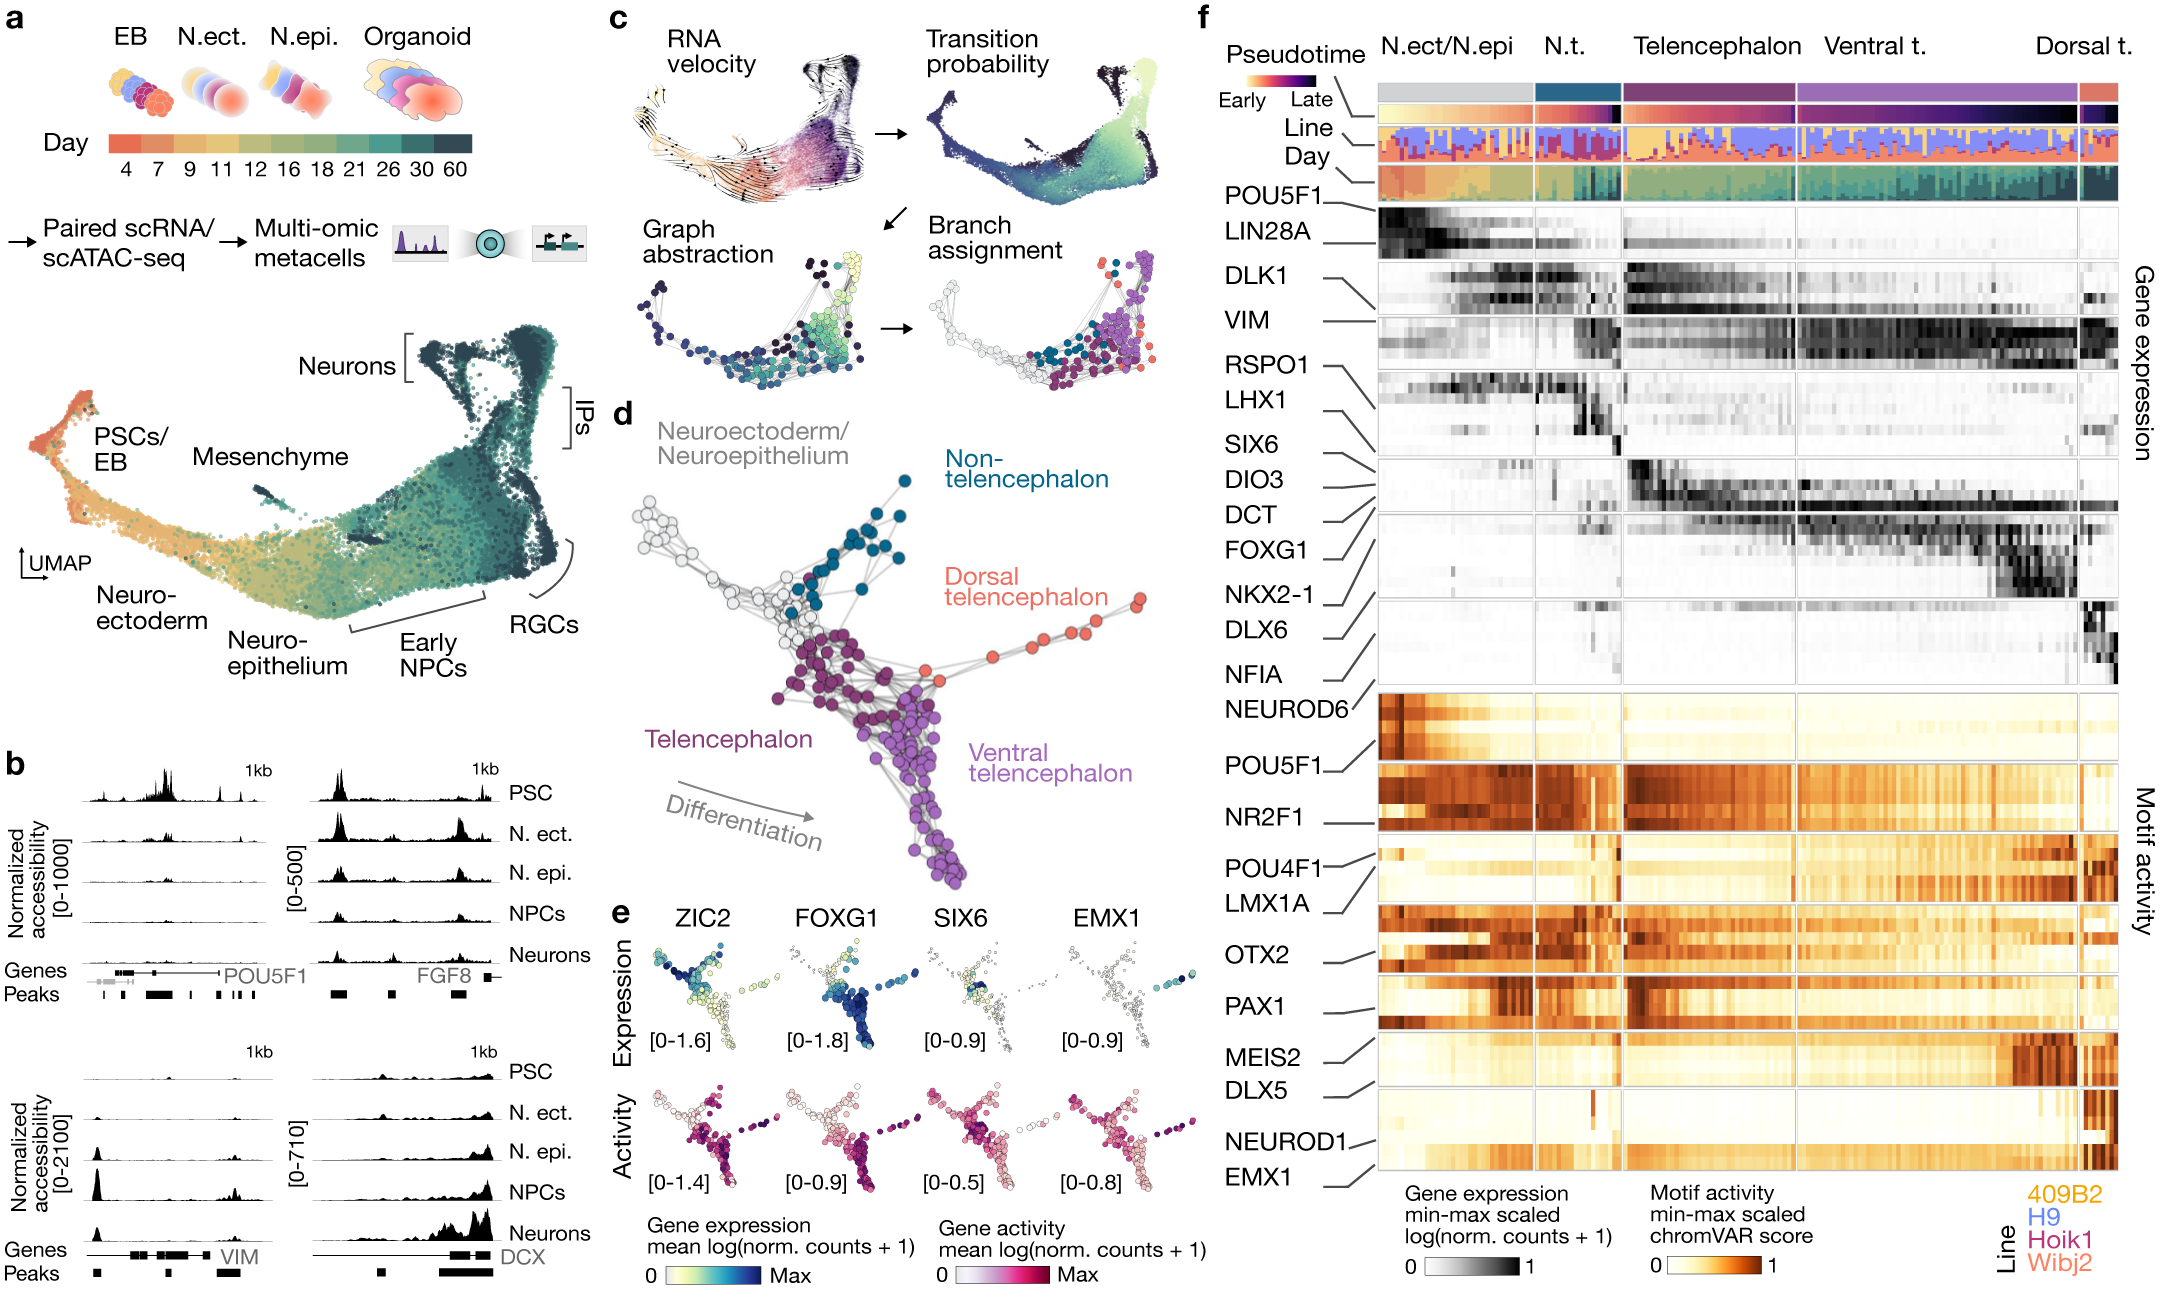
\includegraphics[width=\textwidth]{figures/pando/Figure_1}
    \caption{\textbf{Multi-omic atlas of brain organoid development reveals developmental hierarchies and critical stages of fate decision.}
    a, Schematic of the experimental design and UMAP embedding of integrated multi-omic metacells. Organoids from four different iPSC lines were dissociated for scRNA-seq and scATAC-seq at timepoints spanning the critical patterning window. The two modalities were integrated to form metacells with RNA and ATAC components. b, Examples of loci that have differential access during organoid development from pluripotency. c, Schematic of branch-inference strategy. High-resolution clusters were assigned to branches based on terminal fate transition probabilities calculated based on RNA velocity. d, Branch visualization in a force-directed layout, with circles representing high-resolution clusters of metacells colored by assignment (Neuroepithelium, gray; Non-telencephalon progenitors, teal; Telencephalon progenitors, plum; Dorsal telencephalon, orange; Ventral telencephalon, purple). e, Graph representation of regional branches colored by mean expression (log(transcript counts per 10k + 1)) (top) and gene activity (log(transcript counts per 10k + 1))  (bottom) of marker genes. The range of values is indicated for each plot. f, Heatmap showing stage- and branch-specific gene expression and motif enrichment z-score calculated with chromVAR {Schep et al., 2017}. Values are min-max scaled across rows.}
    \label{fig:reg1}
\end{figure}

\topparagraph{Single-cell multiomic reconstruction of cerebral organoid development}
To explore mechanisms underlying human brain development, we generated single-cell transcriptome and single-cell accessible chromatin profiling data over a time course of cerebral organoid development (Figure 3.1a, Figure S3.1a, Supplementary Table 3.1). The dataset incorporates 11 time points from four human iPSC lines covering two months of development spanning embryoid body (EB) formation, neuroectoderm induction, neuroepithelialization, neural progenitor patterning, and neurogenesis. At each time point, organoid tissues from the four lines were dissociated and scRNA-seq and scATAC-seq pipelines (10X Genomics) were run on the same cell suspension. The sequencing data was demultiplexed using single nucleotide variants (SNVs) specific to each individual and the two modalities for each line and time point were integrated using canonical correlation analysis (CCA) (\cite{stuart_comprehensive_2019}) (Figure S3.1b-f, Supplementary Table 3.2). We constructed ‘multi-omic metacells' containing information on both transcriptome and chromatin accessibility using minimum-cost, maximum-flow (MCMF) bipartite matching (\cite{stark_scim_2020}) within the CCA space (Figure S3.1b,g-h). We evaluated the integration using a multiome dataset, where transcriptome and accessible chromatin were measured within the same cell, and observed strong correlation (Figure S3.1i,j). The metacells were integrated using cluster similarity spectrum (CSS)(\cite{he_css_2020}), and the integrated data was visualized using a Uniform Manifold Approximation and Projection (UMAP) embedding. This revealed a relatively continuous distribution of cell states through the entire time course (Figure 3.1a). Organoid development proceeds from pluripotency (e.g. POU5F1) via a neural progenitor cell state (e.g. PAX6, VIM) to progenitor and neuron cell states of the dorsal telencephalon (e.g. EMX1, NEUROD6), the ventral telencephalon (e.g. DLX5, ISL1, GAD1), of non-telencephalic regions (e.g. TCF7L2, LHX9), and of a small mesenchymal population (e.g. DCN, COL5A1), with cells from the different lines largely intermixed (Figure S3.1f,k). The high-dimensionality of the data could be used to identify marker genes and gene regulatory regions for the different cell states (Figure 3.1b, Figure S3.1l, Supplementary Table 3.3). We observed a pseudotemporal cascade of chromatin accessibility changes over the developmental time course associated with genes involved in stem cell maintenance, neural tube patterning, morphogenesis, neural precursor proliferation, neuron fate specification, and other relevant biological processes (Figure S3.1m, Supplementary Table 3.4).

Previous studies have described the emergence of patterning centers within the neuroepithelium which coordinate to regionalize the developing organoid (\cite{renner_self-organized_2017}). To reconstruct the earliest events involved in cell fate restriction, we sub-clustered early portions of the trajectory and identified molecular heterogeneity (Figure S3.2). In the initial stages (day 7-9), we observed a predominant neuroectodermal population (SIX3, CDH2, SOX3, HES5) and a minor population of cells expressing non-neural ectoderm markers (DLX5, TFAP2A)(\cite{mittnenzweig_single-embryo_2021,ealy_single-cell_2016}) (Figure S3.2a-c). After day 9, cells differentiate into a neuroepithelial population (LDHA), which later diverges into neural progenitor cells (NPCs) expressing either telencephalic (FGF8) and non-telencephalic markers (WLS, WNT8B), followed by a second divergence into dorsal (BMP7, EMX1) and ventral telencephalic NPCs (DLX2; Figure S3.2d-f). RNA fluorescent in situ hybridization (RNA-FISH) using hybridized chain reactions (HCR) of whole-mount 18 day old organoids confirmed the expression and spatial segregation of some of these regional markers (Figure S3.2g).

To assess neuroepithelial self-patterning variation across stem cell lines, we collected additional single-cell multiome data including transcriptome and accessible chromatin modalities for a total of 9 lines (iPSCs: 409B2, B7, HOIK1, KUCG2, WIBJ2, WTC; ESCs: H1, H9, HES3) (~3 weeks; Figure S3.3a). Heterogeneity analysis and comparison with a single-cell transcriptomic atlas of the developing mouse brain6 revealed transcriptionally distinct clusters organizing along an anterior-posterior axis (Figure S3.3b). These clusters expressed many transcription factors, secreted ligands and surface receptors associated with patterning centers such as hypothalamic floor plate (SIX6, HES5, SIX3), roof plate (FGFR3, RSPO3, WNT7B) and hindbrain roof plate (MSX1, BAMBI, BNC2; Figure S3.3c). Notably, marker expression was consistent between lines, however cluster proportions varied substantially, consistent with previous reports(\cite{kanton_organoid_2019}). We further identified cluster-specific candidate cis regulatory elements (CREs) of patterning-related genes and found that many were similarly accessible across lines (Figure S3.3d). These data suggest interesting variation between lines in the propensity to self-pattern, and also support a preserved GRN underlying brain region formation.

We next sought to reconstruct the neurogenic differentiation trajectories for each brain region. We used RNA velocity (\cite{manno_rna_2018,bergen_generalizing_2020}) and CellRank (\cite{lange_cellrank_2022}) to generate a terminal fate transition probability matrix based on transcriptomes, which we used to construct a differentiation graph of high-resolution metacell clusters and assign branch identities (Figure 3.1c, Figure S3.4a-e). The graph, presented by a force-directed layout, reveals an early bifurcation into anterior telencephalic and posterior non-telencephalic cell states and later branching of telencephalic progenitors into dorsal excitatory and ventral inhibitory neuronal trajectories, respectively (Figure 3.1d,e). This telencephalic progenitor state prior to dorsoventral divergence is marked by the expression of DCT, DIO3 and SIX6 and is characterized by transient accessible chromatin regions (Figure 3.1f). Transcriptional and regulatory dynamics can be explored along each neurogenic trajectory, revealing regional specificity of gene expression, chromatin accessibility and binding motif enrichment for stage-specific transcription factors (Figure 3.1f, Figure S3.4f,g). Altogether, this data provides a multi-omic developmental atlas spanning the course of brain organoid regionalization and neurogenesis.
 


\topparagraph{A gene regulatory network view of human cerebral organoid formation}
To infer the GRN underlying human cerebral organoid development, we developed an algorithm called Pando (Figure 3.2a, see Methods), which leverages multi-modal single-cell genomic measurements and models gene expression through TF-peak interactions. Pando first identifies candidate regulatory regions that show accessibility across the organoid time course by incorporating information on conservation (\cite{siepel_evolutionarily_2005}) and previous cis-regulatory element (CRE) annotations (\cite{encode_project_consortium_expanded_2020}) (candidate regions, Figure S3.5a,b). We performed Cleavage Under Targets and Tagmentation (CUT\&Tag) of the H3K27ac histone modification marking active promoters and enhancers to assess regulatory region selection performance. We found that 94\% of accessible peaks intersecting with H3K27ac were among the candidate regions, indicating a strong enrichment for active regulatory regions (Figure S3.5a). 
\begin{figure}[t!]
    \centering
	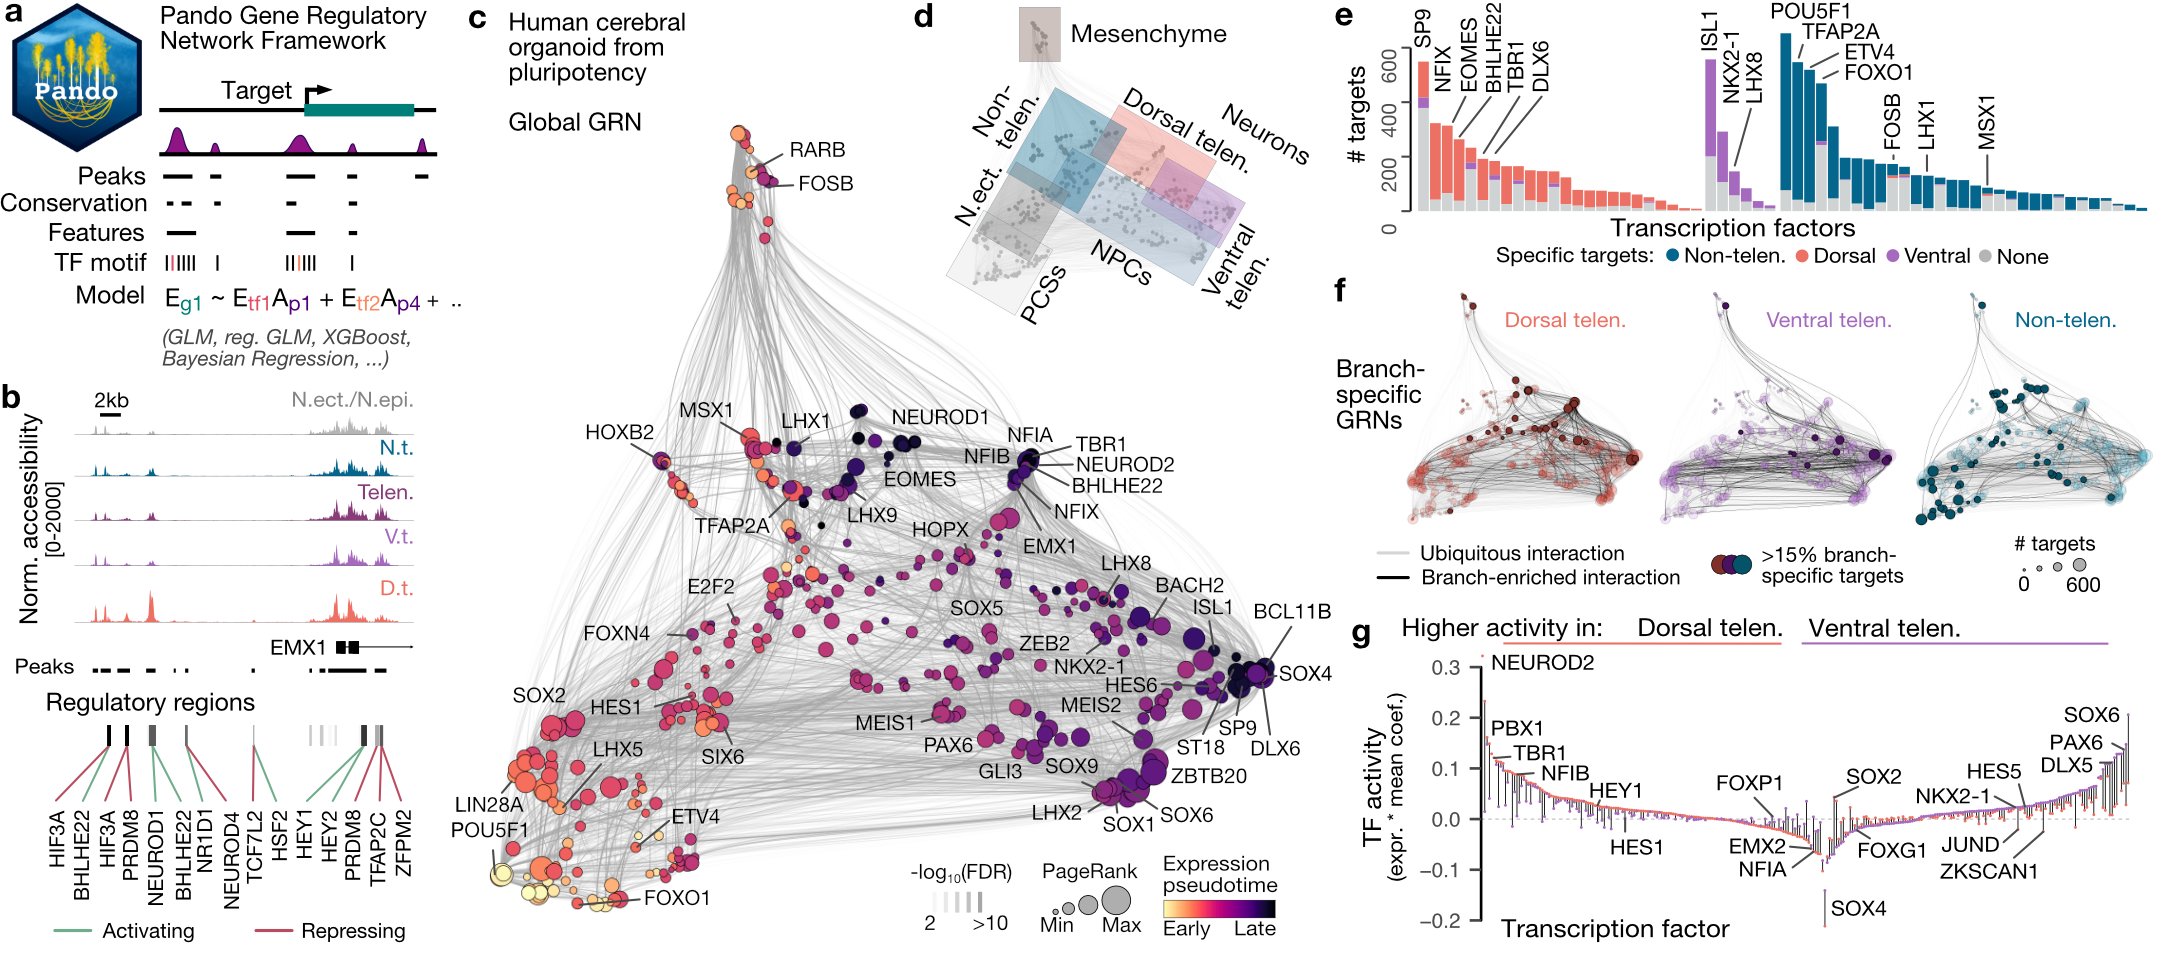
\includegraphics[width=\textwidth]{figures/pando/Figure_2}
    \caption{\textbf{Pando leverages multimodal measurements to infer a multi-phasic gene regulatory network underlying human brain organoid development.}
    a, Schematic of the Pando GRN-inference framework. Candidate regions are identified through intersection of accessible peaks with cis-Regulatory Elements (CREs) or conserved elements. Predicted TFs are selected for each candidate region through binding motif matching. The relationship between TF-binding site pairs and expression of target genes is then fit with a regression model. b, Signal tracks showing normalized accessibility at the transcription start site of EMX1 in the different branches and inferred regulatory regions for various transcription factors. Line color represents the sign of the interaction and box color (grayscale) represents the FDR of the most significant interaction for this region. c, UMAP embedding of the inferred TF network based on co-expression and inferred interaction strength between TFs. Color and size represent expression weighted pseudotime and PageRank centrality of each TF, respectively. d, UMAP embedding shaded by module features. e, Barplots showing target specificity for branch-specific TFs. f, UMAP embedding of branch-specific TF networks highlighting TFs with branch-specific targets and interactions with branch-specific accessibility. g, Plot shows groups of TFs with differential activity between the dorsal (red) and ventral (purple) telencephalon branch. TF activity is indicated by a colored dot for each branch, connected by a line, and was calculated by multiplying the mean regulatory coefficient with the average expression in the branch. The sign of the activity indicates whether the regulation is mainly activating (+) or repressing (-).}
    \label{fig:reg2}
\end{figure}
Next, candidate regions are assigned to genes in their vicinity and TF binding sites are predicted for each region (Figure S3.5c-e). Linking regulatory regions to genes based on proximity has limitations, however it is an effective assumption for many regulatory interactions at the genome scale (\cite{mclean_great_2010,aibar_scenic_2017}), and we observed strong correlation between gene expression and a regulatory domain that includes proximal promoter and gene body regions (Figure S3.1i). Pando then uses a regression model to infer the relationship between the expression of each target gene, TF expression and binding site accessibility (Figure 3.2a, Figure S3.5f). As a consequence, Pando jointly infers sets of positively or negatively regulated target genes (gene modules) as well as regulatory genomic regions (regulatory modules) for each TF (Figure 3.2b, Figure S3.5g-i). We visualized the GRN using a UMAP embedding, which revealed groups of TFs that are involved in different phases of cerebral organoid development, broadly representing the pseudotemporal order of cell state transitions (Figure 3.2c). A series of TFs tracked transitions from pluripotency (e.g. POU5F1, LIN28A) to neuroepithelium induction (e.g. SOX2, HES1), with additional module neighborhoods linked to brain regional NPC specification and neuron differentiation (Figure 3.2d, Figure S3.5j,k). Nodes associated with initializing (pluripotency) and terminal states (regionalized neurons) had a high degree of centrality, reflecting the high number of correlated expressed genes for these states. We found certain TF modules to be pseudotime-dependent independent of brain regional identity (e.g. SP9, SCRT1), whereas others showed specificity for a given brain region (e.g. EMX1, NR1D1, NEUROD6 in dorsal telencephalon; IRX5 in non-telencephalon) (Figure S3.5j,k). Globally, this GRN shows that regulatory region accessibility and TF expression track with stages of organoid development and segregate during brain regionalisation.

To better understand how chromatin accessibility constrains and specifies GRN activity in different brain organoid regions, we next analyzed differential accessibility of inferred binding sites between regional branches. We pruned regulatory edges with strongly depleted accessibility and could identify TFs with highly branch-specific target sets (Figure 3.2e). We further partitioned the global GRN into branch-specific GRNs (Figure 3.2f), representing subgraphs whose activity is shaped by changes in chromatin accessibility between branches. Within these subgraphs, we computed TF activity as the mean coefficient of all active connections multiplied by the mean expression in the branch (Fig 2g). Comparing TF activity in the dorsal and ventral telencephalon branch revealed TFs with high branch-specificity (e.g. NEUROD2, NFIA, SOX6) as well as TFs whose mode of regulation changed between mainly activating (positive activity) to mainly repressing (negative activity; e.g. HEY1, JUND, ZKSCAN1) and vice versa (e.g. SOX2). Altogether, these analyses provide a rich resource for future work to understand the gene regulatory programs controlling human brain regionalization and TF-mediated cell programming.


\topparagraph{Single-cell genomic perturbation of cortical transcription factors in organoids}
To begin to understand the mechanisms regulating cell fate and state during human brain development, we employed a pooled perturbation screen17 in mosaic organoids (Figure 3.3a). We designed gRNAs and generated a pooled lentiviral library targeting 20 TFs (each targeted by 3 gRNAs) expressed in different stages of both organoid and primary developing human cortex7 and with no expression in iPSC or neuroectoderm stages (Figure 3.3b, Figure S3.6a,b). We transduced iPSCs harboring an inducible Cas9 cassette with the lentiviral gRNA library, and sorted and expanded vector positive iPSCs based on fluorescence (Figure S3.6c). We induced Cas9 expression in the infected iPSCs expressing different gRNAs, and used the mosaic pool of iPSCs to generate mosaic cerebral organoids containing a multitude of perturbed genotypes. Fluorescence was maintained throughout organoid development, and bulk amplicon sequencing revealed relatively homogenous detection of the gRNAs (Extended Data Figs. 6d and 7a). At day 60, at which neural progenitors and neurons coexist in the organoid and all targeted TFs have been or are being expressed (Figure 3.3b and Figure S3.6a-b), we dissociated the mosaic organoids and sequenced single-cell transcriptomes and guide cDNA amplicons of 3 individual organoids as well as a pool of multiple organoids. We recovered 22,449 cells with an assigned gRNA. Each gRNA for all 20 targets was detected with an average of 1 gRNA detected per cell (Figure 3.3c, Figure S3.7b-e). We generated a UMAP embedding, analyzed cell type heterogeneity, and annotated NPCs, intermediate progenitors, and neurons in the dorsal telencephalon, the ventral telencephalon, as well as in non-telencephalic developing brain regions (Figure 3.3d, Figure S3.7f-i).

\begin{figure}[b!]
    \centering
	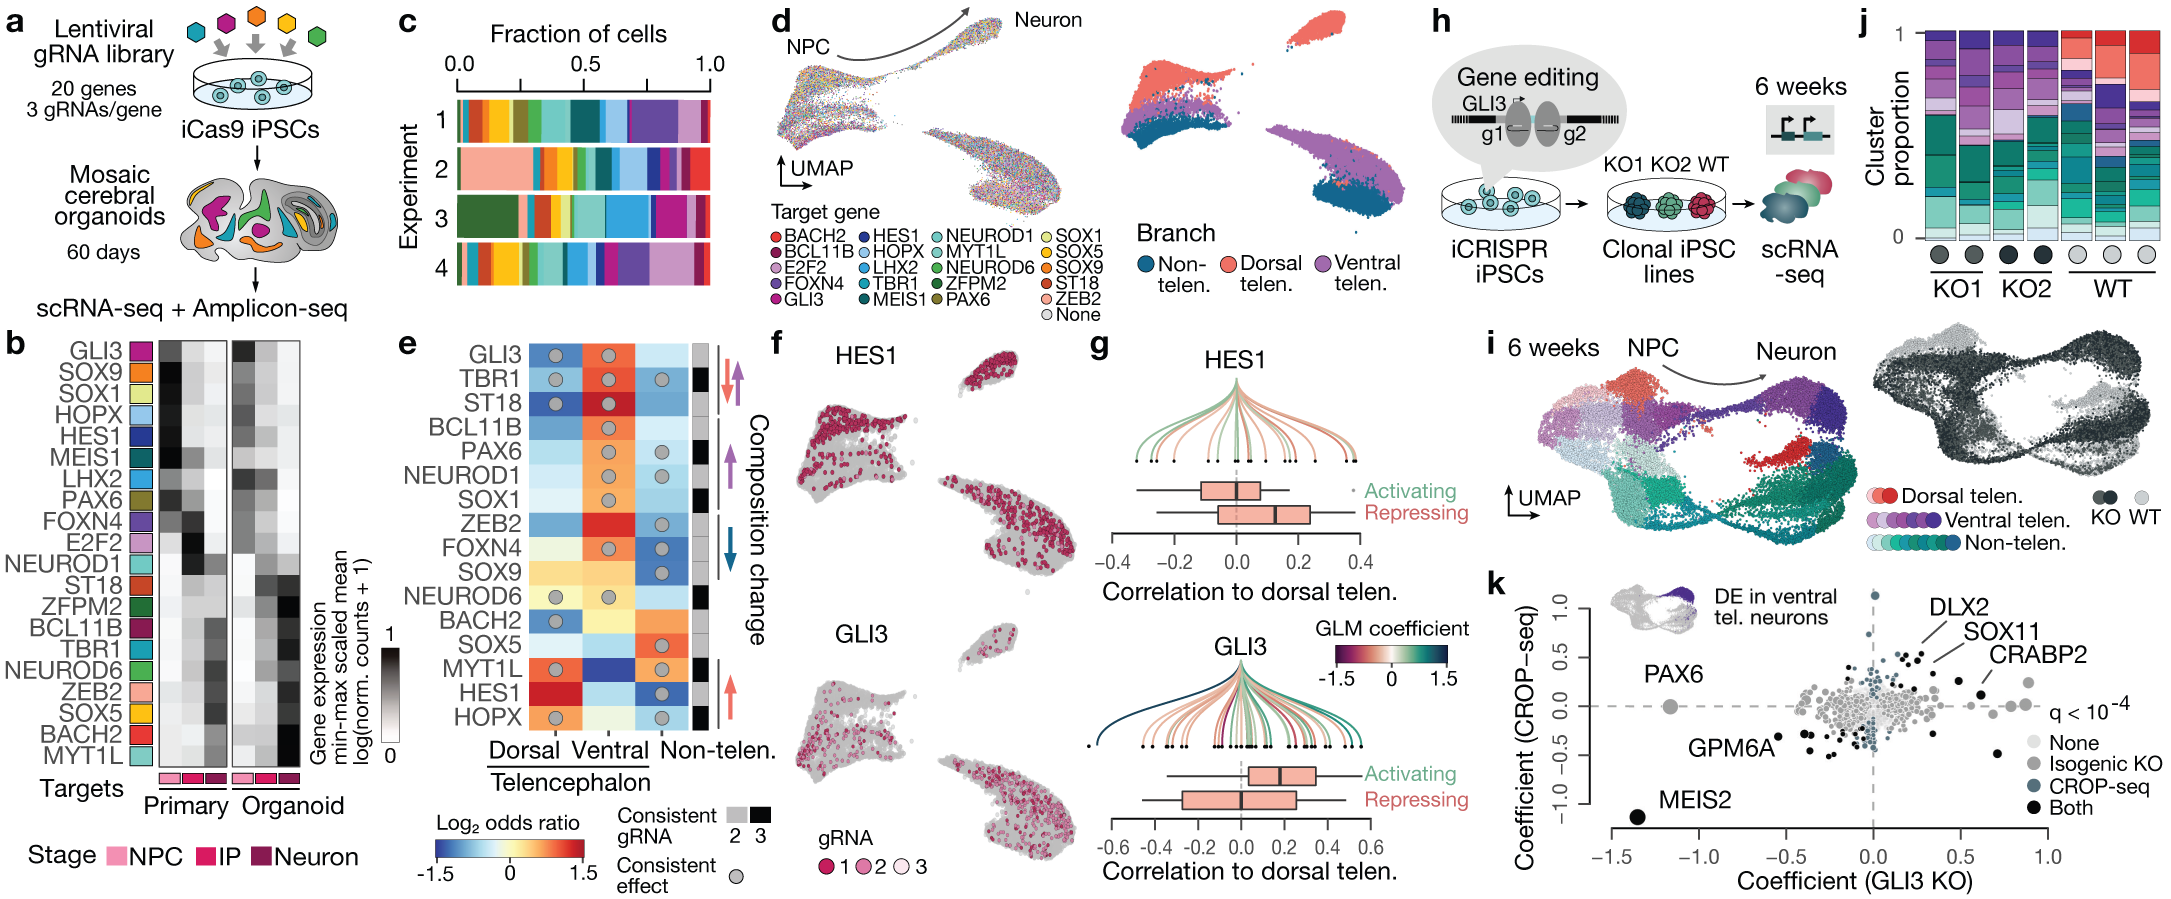
\includegraphics[width=\textwidth]{figures/pando/Figure_3}
    \caption{\textbf{Transcription factor perturbations in mosaic organoids reveal critical regulators of neurodevelopmental fate decisions.}
    a, Schematic of single-cell perturbation experiment using the CROP-seq method and data analysis. b, Heatmap showing min-max scaled average expression (log(transcript counts per 10k + 1)) of targeted genes in neural progenitor cells (NPC), intermediate progenitors (IP) and neurons of the primary and organoid cortex. c,  Barplot showing the proportion of cells with each perturbation for each experiment. d, UMAP embedding with cells colored by detected gRNA (left) and branch assignment (right). e, Heatmap showing regional enrichment of gRNAs. Sidebar shows the number of gRNAs that were consistent and circles represent consistent effects between experiments and statistically significant (FDR<0.01) effects on composition. Arrows indicate the predominant observed effect. f, UMAP embedding colored by consistent gRNAs for selected genes that had a strong effect on fate regulation. g, Box plots showing the spearman correlation of HES1 (top, n=18 genes) and GLI3 (bottom, n=42 genes) target genes to transition probabilities into the dorsal branch. The GRN was subsetted to retain connections accessible at the branchpoint (>5\% detection rate). The center line represents the median, boxes indicate the 25\%-75\% interquantile range and whiskers indicate 1.5 * interquantile range. h, Schematic of GLI3 loss of function experiment (knock-out, KO; wild-type, WT) using the iCRISPR nickase system. i, UMAP embedding showing trajectories from neural progenitor cells (NPCs) to neurons colored by different clusters assigned to regional branches, with inset colored by genetic condition. j, Stacked barplots showing distribution of cluster assignment per organoid for each condition, colored by cluster. k, Differential expression (DE) in ventral telencephalic neurons for GLI3 KO and CROP-seq data containing a GLI3 gRNA. X and y axes indicate coefficients of the linear model. Colors indicate significance (FDR<$10^{-4}$) in CROP-seq, KO cell line, or both.}
    \label{fig:reg3}
\end{figure}

We tested the association of gRNA detection on cell type abundance and on differential gene expression within cell types (Figure S3.8). We first hierarchically clustered Louvain clusters based on gRNA abundance and observed grouping by brain region (Figure S3.8a). This showed that different brain regions exhibited unique gRNA compositions suggesting region specific effects of TF perturbations. Next, we stratified the detected gRNAs using a log odds ratio (p-value based on a Cochran–Mantel–Haenszel test) and assessed the consistency of the effect across organoids and gRNAs (Figure S3.8b, Supplementary Table 3.5). Based on these metrics, we found that gRNAs targeting 8 TFs showed consistent enrichment in the ventral telencephalon branch with corresponding depletion in the other regions, including the cortex (Figure 3.3e; e.g. GLI3, TBR1). Another set of perturbations showed the opposing effect, with enrichment of TF targeting gRNAs in the cortex and depletion in either ventral telencephalon or non-telencephalon (e.g. HES1, HOPX). We focused on HES1 and GLI3, two genes which are expressed at the dorsoventral branchpoint and show opposing effects on dorsal telencephalon commitment (Figure 3.3e,f). Both genes are known regulators of mouse cortical development (\cite{nakamura_bhlh_2000,wang_gli3_2011,hasenpusch-theil_gli3_2018}), and are associated with developmental disorders in humans (\cite{song_non-coding_2021,biesecker_greig_2008}). We used the GRN inferred from the developmental time course to investigate how GLI3 and HES1 target gene expression correlates with transition probabilities into dorsal telencephalon (Figure 3.3g). We found that genes activated by GLI3 were positively correlated with cortical transition probabilities, while HES1 had a repressive effect on such genes. This suggests an antagonistic involvement of these two genes in shaping the dorsoventral fate decision in the human telencephalon. Of note, we also found that for several TFs perturbation led to detectable transcriptomic effects rather than composition changes (Figure S3.8c-f, Supplementary Table 3.6 and 7). In particular, E2F2, a crucial cell cycle regulator (\cite{swiss_cell-context_2010}), altered the transcriptome of both dorsal and ventral telencephalic neurons suggesting that misregulation of cell cycle exit has a large effect on the neuronal transcriptome state. Altogether, these data provide one of the first implementations of an in organoid multiplexed perturbation experiment to explore the effect of genetic perturbations on human brain cell fate and state development.


\topparagraph{GLI3 directly targets HES regulomes during human organoid telencephalon development}
Mosaic perturbations suggested that GLI3 is involved in dorsoventral neuronal fate specification in the human telencephalon. GLI3 is a well known mediator of Sonic Hedgehog (SHH) signaling (\cite{ruiz_i_altaba_hedgehoggli_2002}), with GLI3 loss of function mutations resulting in failure of the cortex to form in mice, and expansion of ventral telencephalic neuronal identities into dorsal locations within the developing brain (\cite{rallu_dorsoventral_2002,theil_gli3_1999}). In humans, mutations in GLI3 have been associated with Greig cephalopolysyndactyly syndrome and Pallister Hall syndrome, in which patients have variable presentations of brain malformations depending on the particular mutations (\cite{biesecker_greig_2008}). To confirm that GLI3 is involved in cell fate establishment in a human context, and to explore the underlying developmental mechanisms, we used CRISPR/Cas9 gene editing to generate two independent GLI3 knock-out (KO) iPSC lines  and a control cell line (WT) that went through the editing process (Figure 3.3h, Figure S3.9a-d). We generated KO and WT cerebral organoids and confirmed that the GLI3 protein is not detected in the KO organoids (Figure S3.9e). We performed scRNA-seq on KO and WT organoids at day 45, a time point of early neurogenesis, and analyzed cellular heterogeneity (Figure 3.3i, Figure S3.9f). Strikingly, KO cells were depleted in the dorsal telencephalon, with a strong enrichment in the ventral telencephalon (Figure 3.3j), and differential gene expression analysis revealed that GLI3 KO impacts ventral telencephalic cell states (Figure 3.3k, Supplementary Table 3.8). Both of these observations were consistent with the mosaic perturbation experiment.


\begin{figure}[b!]
    \centering
	\includegraphics[width=\textwidth]{figures/pando/Figure_4}
    \caption{\textbf{Single-cell multiome view of GLI3 loss of function reveals distinct regulomes and novel effectors of dorsoventral telencephalon specification.}
    a, Schematic of the experiment where transcriptome and chromatin access was measured in the same cell at 3 weeks of cerebral organoid development. b, UMAP embedding colored by cluster and labeled by projected cell fate. Inset UMAP colored by genetic state. c, Lollipop plot showing number of DEGs of control (WT) versus GLI3 KO cells in the different clusters. d, Volcano plot showing DE in telencephalic progenitors (cluster 0 and 2) upon GLI3 KO. e, Heatmap showing DEGs upon GLI3 KO for early telencephalic progenitors (week 3), ventral telencephalic progenitors (week 6) and neurons (week 6), and differential accessibility (DA) upon GLI3 KO in early telencephalic progenitors (week 3). All genes are colored by the related signaling pathway (if applicable) and molecular function. f,g, Subgraph of the GRN for early telencephalic progenitors (f) and in the ventral telencephalon (g), showing direct and second-order GLI3 targets. Circles are genes with all TFs being labeled. Edges are colored based on regulatory interaction by the TF. h, GLI3 binding score (sum of C\&T signal intensity for gene body + 2kb) in WT organoids versus DE log fold change in early telencephalic progenitors (week 3). Genes with differentially accessible Cis-regulatory elements (CREs) are colored black. Signal tracks of GLI3 binding matched with DA peaks of HES4 and HES5 in early telencephalic progenitors. i, Z-scored mean correlation between module genes expression and branch probabilities (branch activation score) for DE TFs. j, Scatterplot showing log fold change of genes upon treatment with SHH versus DE in GLI3 KO. GO terms are shown for common DEGs, SHH treatment specific and GLI3 specific DEGs. k, Schematic summarizing the results from GLI3 and SHH perturbations.}
    \label{fig:reg4}
\end{figure}


Interestingly, the TF MEIS2, a marker of lateral/caudal ganglionic eminence (LGE/CGE) relative to medial ganglionic eminence (MGE), was strongly down-regulated in GLI3 KO conditions (Figure 3.3j). Further analysis on the ventral telencephalic neuron heterogeneity identified distinct LGE/CGE-like and MGE-like neuronal populations with GLI3 KO cells strongly enriched in MGE neurons (Figure S3.9g,h). We observed expression alterations in GLI3 KO LGE-like neurons compared to the WT LGE state with genes involved in dorsoventral patterning (PAX6, MEIS2, DLK1) being differentially expressed (Figure S3.9h). These data confirm that GLI3 is necessary for cortical neuron fate establishment in humans, and its absence impacts ventral telencephalon development by promoting MGE neurogenesis and altering LGE neuronal expression, consistent with a role in MGE fate repression (\cite{sousa_sonic_2010}) and LGE neuron state regulation (Figure S3.9h,i).
GLI3 is expressed broadly in progenitors of the telencephalon and of non-telencephalic regions (Figure S3.4f), suggesting distinct GLI3 regulatory roles during different phases of brain development. We therefore generated single-cell multiome data (10X Genomics) of WT and GLI3 KO organoids at a time point (3 weeks) preceding dorsoventral patterning (Figure 3.4a, Figure S3.10a-c). WT and GLI3 KO organoids showed comparable cell composition (Figure 3.4b), however strong differential expression and differential accessibility was detected between KO and WT cells in the telencephalic progenitor population (cluster 0 \& 2, Figure 3.4b,c, Supplementary Table 3.9). Differentially expressed genes (DEGs) included HES1 (up-regulated) and HES4/HES5 (down-regulated) (Figure 3.4d, Figure S3.10d) as well EMX2 (down-regulated). Interestingly, GLI3-KO cells showed upregulation of SOX4 and SOX11, two genes detected as downregulated in HES1-perturbed cells in the CROP-seq experiment, consistent with the opposing effect of GLI3 and HES1 on dorsal telencephalic fate emergence (Figure 3.3e, Figure S3.10e).
Combining single cell data of WT and GLI3 KO organoids of both time points (3 and 6 weeks) revealed TFs and signaling pathways differentially expressed specifically in telencephalic progenitors, ventral telencephalic NPCs and ventral telencephalic neurons (Figure 3.4e), hinting towards a distinct regulatory role of GLI3 in these different developmental stages. In telencephalic progenitors, GLI3 KO leads to upregulation of FGF-related genes (FGF8, SPRY1, FGF13) and a down-regulation of WNT-related genes (WNT7B, WNT5B, LGR5), while ventral telencephalic cells showed dysregulation of hedgehog pathway receptor PTCH1 and several transcription factors including NKX2-1, EMX2, GSX2 and ID1. GLI3 KO induced differential accessibility (DA) of CREs linked to these genes and pathways (Figure 3.4e and Figure S3.10f-g, Supplementary Table 3.10 and 11). Interestingly, many genes were differentially expressed only in the later ventral telencephalic stages, whereas CREs were DA already in telencephalic progenitors (e.g. NKX2-1, ID1), indicating a potential priming effect.

We explored the perturbation signatures in the context of our inferred GRN, and observed strong consistency between GLI3 direct and indirect targets and detected DEGs, supporting predictability of the GRN (Figure 3.4f,g, Figure S3.10h-k). Two GLI3 sub-GRNs describe distinct perturbation effects in telencephalic progenitors and in the ventral telencephalon branch, respectively (Figure 3.4f,g). Prior to dorsoventral fate bifurcation, the sub-GRN suggests GLI3 directly activates HES4, HES5, PAX6, OTX2 and CREB5, with 76\% of the DEGs being indirect targets of GLI3. After specification of the ventral telencephalon, a second sub-GRN suggests GLI3 directly regulates PAX6, LHX8, ID1 and BCL11A. GLI3 CUT\&Tag in 3 week old organoids revealed extensive GLI3 binding at genomic regions nearby HES4, HES5, CREB5 and PAX6 that also show DA in GLI3 KO cells, confirming that GLI3 binds these targets directly in telencephalic progenitors (Figure 3.4h). Interestingly, even though HES4/5 can be targets of the Notch pathway, we did not observe enrichment for other NOTCH targets, suggesting independence of Notch signaling (Figure S3.10m). We assessed the relevance of GLI3 targets in driving dorsal or ventral telencephalic fate establishment by computing a dorsal and ventral telencephalon branch activation score for each TF module (Figure 3.4h, Figure S3.10l). This analysis suggests that GLI3 targets HES5, EMX2 and PAX6 are major drivers of dorsal telencephalic fate, while FOXG1 and DMRTA1 activate ventral telencephalic fate.

Finally, we wanted to understand the interplay between GLI3 and SHH, a major inducer of telencephalon ventralization (\cite{echelard_sonic_1993,ericson_sonic_1995}). Organoids were treated with SHH for 3 days during the neuroepithelial stage (3 weeks) followed by multiome profiling. Differential expression analysis revealed down-regulation of GLI3 in SHH treated versus untreated control telencephalic progenitors (Figure S3.10n-o), and overall there was highly significant correlation with GLI3 KO-induced DEGs (Figure 3.4j, Pearson's r: 0.5). GO analysis showed that shared and GLI3-specific DEGs were enriched in brain regionalization and differentiation-related genes, while SHH-specific DEGs were largely lipid metabolism-related. This suggests that SHH promotes ventralization predominantly by preventing GLI3-induced dorsalization (\cite{rallu_dorsoventral_2002,rash_patterning_2007}). Taken together, our data-driven approach provides a multiphasic GLI3 gene regulatory model for human telencephalon development that is consistent with previous studies, while also proposing novel downstream effectors (Figure 3.4k).


\subsection{Discussion}
The human brain has unique features that distinguish it from other species. Despite the high-resolution descriptions of mouse and human developing brain cell composition from recent cell atlas efforts (\cite{nowakowski_spatiotemporal_2017,trevino_chromatin_2020,la_manno_molecular_2021}), it has been a major challenge to study the mechanisms that control human brain development due to difficulty in obtaining tissue at the earliest stages of brain patterning, and the lack of methods to systematically manipulate gene function. Here we have integrated transcriptome, chromatin accessibility, and genetic perturbation datasets to provide insight into the mechanisms underlying human brain regionalization. In a broad sense, we find that the programs identified in mouse and other non-human model systems are well conserved in humans, and the extent that stem cell-derived cerebral tissues recapitulate these programs is remarkable. We focused on GLI3 as a well-studied transcription factor controlling dorsoventral fate specification in the rodent telencephalon. We find clear and striking evidence that this same transcriptional program is well-conserved in humans. More importantly, this data provides strong evidence that multi-region human brain organoids can be predictive model systems. We note that unguided neural organoid protocols result in strong variation between stem lines with regard to proportions of regions represented in each organoid or batch. We find that chromatin accessibility showed higher line-specificity than gene expression, which might have indications for the epigenetic state of the reprogrammed line and subsequent propensity for forming certain brain regions.

We established the Pando GRN inference framework which incorporates features of the regulatory genome that have not been previously utilized for global analysis of developmental programs. Pando generalizes regression-based GRN inference for multimodal datasets by combining transcriptome, chromatin accessibility, an expanded TF family motif reference, known cis-regulatory elements, and evolutionary conservation into a flexible framework. The R package implements the full GRN inference strategy including candidate region selection, motif matching, model fitting and discovery of gene and regulatory modules. Further, it offers a wide range of regression models to be used for GRN inference. We have highlighted interesting aspects of the network, such as TF modules involved in the transition from pluripotency via neuroectoderm to a neuroepithelium, as well as the subnetworks associated with regionalized brain states. The latter will be interesting to explore in experiments designed to program specific neuronal states, or to systematically perturb human organoids. We note that current limitations include the lack of comprehensive active and repressive histone modification and chromatin conformation status across organoid development, as well as incomplete TF motif databases. We expect these to be an active area of research, and Pando has the flexibility to include such priors into the GRN inference framework.

We validated the critical role of GLI3 in dorsal telencephalic cell fate specification in humans, and further identified the contribution of GLI3 during specification of MGE and LGE/CGE neurons. The integration of the single-cell multiome data from GLI3 KO organoids and the global GRN suggested a model in which GLI3 becomes induced in early telencephalic NPCs through SHH signaling during neuroepithelial regionalization. GLI3 then regulates downstream targets, activating cortical fate acquisition through differential activity of HES5, HES4 and HES1 and inhibiting the MGE induction program through regulation of BCL11A, LHX8, NKX2-1. Our data also suggests that GLI3 can regulate HES genes directly, likely through NOTCH-independent mechanisms similar to what has been described recently during mouse limb development (\cite{sharma_hes1_2021}). More broadly, our data reveals the extraordinary potential of multi-modal single-cell genomic and organoid technologies to understand gene regulatory programs of human brain development.


\subsection{Methods}

\paragraph{Acknowledgements}
We thank the Camp and Treutlein labs, as well as Fabian Theis' lab for helpful discussions. We thank Eveline Ilcken, Anne Weigert, Sabina Kanton and Theresa Schaffer for assistance with stem cell and organoid culture and Tobias Gerber, Leila Sidow, and Keisuke Sekine for discussions relating to cloning. We thank Stephan Riesenberg and Svante Pääbo for kindly providing the iCRISPPR cell lines, the Institute for Ophthalmology Basel for providing the 01F49i-N-B7 cell line, and the Murdoch Children's Research Institute and Murdoch University for providing the HES-3 NKX2.1GFP/w cell line. We thank Michael Dannemann and Tomislav Maricic for providing genotype information for demultiplexing. Illumina sequencing was done by Barbara Schellbach and Antje Weihmann at the Max-Planck-Institute for Evolutionary Anthropology and Ina Nissen, Elodie Vogel Burcklen and Christian Beisel of the Genomics Facility at D-BSSE, ETH Zurich. FACS sorting support was provided by Mariangela Di Tacchio, Aleksandra Gumienny, Renan Antonialli and Thomas Horn of the single-cell facility at D-BSSE, ETH Zurich. We thank 10X Genomics for support with multiome experiments. No research with human ESC lines was funded by the ERC. This work was supported by Chan Zuckerberg Initiative DAF, an advised fund of the Silicon Valley Community Foundation CZF2019-002440 (J.G.C., B.T.), the European Research Council (Anthropoid, J.G.C.; Organomics, B.T.; Braintime, B.T.), the Swiss National Science Foundation (Project Grant-310030\_84795, J.G.C.; Project Grant-310030\_192604, B.T.) and the National Center of Competence in Research Molecular Systems Engineering (B.T.). J.S.F was supported by the Boehringer Ingelheim Fonds.
 
\paragraph{Author contributions} S.J. generated organoids used in this study, with support from J.S.F., R.O. and D.W.. S.J. generated all single-cell transcriptome and accessible chromatin datasets with support from M.Sa.. S.J. performed the CROP-seq and the multiome experiments. J.S.F., D.W., M.Se. constructed CROP-seq vectors. S.J. generated the GLI3 iPSC lines and generated the scRNA-seq data on GLI3 KO organoids with help from D.W.. F.Z., S.J. performed western blots for GLI3. F.Z. performed the Cut\&Tag experiment. S.J., A.J. generated IHC and HCR data. J.S.F. performed the analysis of the scRNA-seq/scATAC-seq developmental time course with support from Z.H., S.J.. J.S.F. developed the Pando R package. J.S.F. analyzed the CROP-seq data with support from Z.H.. S.J., J.S.F. analyzed the GLI3 KO scRNA-seq and multiome data. J.S.F., S.J., Z.H., J.G.C., B.T. designed the study and wrote the manuscript..
 
\paragraph{Competing interests} The authors do not declare any conflicts of interest.

\paragraph{Correspondence and requests for materials} should be addressed to Z.H., B.T. or J.G.C.
 
\paragraph{Data availability} Raw sequencing data is available on ArrayExpress. The accessions for the individual experiments are E-MTAB-12001 for developmental time course scRNA-seq data, E-MTAB-11998 for developmental time course scATAC-seq data, E-MTAB-12004 for multiome data of the neuroepithelial stage, E-MTAB-11999 for scRNA-seq data of the CROP-seq experiment, E-MTAB-12005 for amplicon sequencing of the CROP-seq experiment, E-MTAB-11997 for scRNA-seq data of GLI3 KO organoids, E-MTAB-12002 for multiome data of GLI3 KO organoids, E-MTAB-12003 for multiome data of SHH-treated organoids and E-MTAB-12006 for Cut\&Tag data. Processed data and the VCF files for demultiplexing are available on Zenodo (https://doi.org/10.5281/zenodo.5242913). The Pando R package is available on GitHub (https://github.com/quadbiolab/Pando). Other custom code used in the analyses is deposited on GitHub (https://github.com/quadbiolab/organoid\_regulomes).
 
 
\paragraph{Stem cell and organoid culture}
We used six human induced pluripotent stem cell (iPSC) lines (Hoik1, Wibj2, Kucg2 from the HipSci resource47; 409B2 from the RIKEN BRC cell bank, 01F49i-N-B7 from Institute of Molecular and Clinical Ophthalmology Basel, and WTC from the Allen Institute) and three human ES cell lines (H1-PAX6YFP and H9 from WiCell and HES-3 NKX2.1GFP/w from the Murdoch Children's Research Institute). Stem cell lines were cultured in mTESR1 (Stem Cell Technologies, 05851) with mTeSR1 supplement (Stem Cell Technologies, 05852) and supplemented with penicillin/streptomycin (P/S, 1:200, Gibco, 15140122) on matrigel-coated plates (Corning, 354277). Cells were passaged 1-2 times per week after dissociation with TryplE (Gibco, 12605010) or EDTA in DPBS (final concentration 0.5mM) (Gibco, 12605010). Media was supplemented with Rho-associated protein kinase (ROCK) inhibitor Y-27632 (final concentration 5$\mu$M, STEMCELL, 72302) the first day after passage. Cells were tested for mycoplasma infection regularly using PCR validation (Venor GeM Classic, Minerva Biolabs) and found to be negative. 4,500 - 5000 cells were plated in ultra low attachments plates (Corning, CLS7007) to generate cerebral organoids using a whole brain organoid differentiation protocol (\cite{lancaster_cerebral_2013}). The use of human ESCs for the generation of cerebral organoids was approved by the ethics committee of northwest and central Switzerland (2019-01016) and the Swiss federal office of public health.

Single cell RNA, ATACseq and multiome experiments for the developmental time course
Cerebral organoids were generated from four different stem cell lines (H9, 409B2, Wibj2, Hoik1) simultaneously. Cerebral organoids of the same batch were dissociated at multiple timepoints of the course of cerebral organoids development. We collected these single cell suspensions from an EB time point (day 4), the time points of neuronal induction (day 7, 9 and 11) and after embedding in matrigel and starting the neuronal differentiation process (day 12, 16, 18, 21, 26, 31 and 61). Organoids of the four different cell lines were pooled based on size and dissociated together and cell lines were later demultiplexed based on the single nucleotide polymorphism (SNP) information. Multiple organoids of each line were pooled together to obtain a sufficient number of cells. For the early time points 15 organoids per cell line were pooled, decreasing this number to minimally 3 organoids for the later time points (Supplementary Table 3.1). For time points just after matrigel embedding, matrigel was dissolved in Cell Recovery Solution (Corning, 354253)​​ for 15 min at 4°C. Organoids were cut in halves and washed three times with HBSS without Ca2+/Mg2+ (STEMCELL technologies, 37250). Single cell suspensions were acquired by dissociation of the organoids with a papain-based dissociation (Miltenyi Biotec, 130-092-628). 2 ml of pre-warmed papain solution was added to the  organoids and incubated for 15 minutes at 37 °C. Enzyme mix A was added before the tissue pieces were triturated 5-10 times with a 1000 wide-bore and p1000 pipette tips.  The tissue pieces were incubated two times for 10 min at 37 °C with trituration steps in between and after with 200 and 1000p pipette tips. Cells were filtered with consecutively 30 $\mu$m and 20 $\mu$m pre-separation filters and centrifuged. Cells were resuspended and viability and cell count were assessed with a Trypan Blue assay on the automated cell counter Countess (Thermo Fisher). Cell suspensions were split in two and resuspended in CryoStor CS10 (STEMCELL technologies, 07952) and cryopreserved at -80 °C. The next day cryotubes were transferred to liquid nitrogen for storage until the scRNA-seq and scATAC-seq experiments were performed.

The cryopreserved single cell suspensions of each time point were thawed by warming up the cryo for 1-2 minutes in a water bath at 37°C and directly centrifuged in 10ml prewarmed DMEM with 10\% FBS. Cells were washed twice with PBS + 5\% BSA and filtered through a 40$\mu$m cell strainer (Flomi). For scATAC-seq, nuclei were isolated according to the protocol provided by 10x genomics (Demonstrated protocol CG000169 Rev D) using the low input protocol and a lysis time of 3 min. Nuclei were loaded in a concentration that would result in a recovery of 10,000 nuclei. In case of less nuclei recovered, the maximum number of nuclei was targeted. Single cell ATACseq libraries were generated with the Chromium Single Cell ATAC V1 Library \& Gel Bead Kit. Prior to sequencing an additional clean-up step was performed to enrich shorter fragments by applying a double sided (1.2-0.75x) cleanup with AMPureXP beads (Beckman Coulter) and Illumina Free Adapter Blocking Reagent was used to reduce potential index hopping. The libraries were sequenced on Illumina's NovaSeq platform.

For sc-RNAseq, cells were put in a concentration after counting and viability checking that allowed targeting 10,000 cells and in case the cell number was not sufficient all cells were loaded. Single cell RNAseq libraries were generated with the Chromium Single Cell 3' V3 Library \& Gel Bead Kit. Single cell encapsulation and library preparation were performed according to the manufacturer's protocol.

To generate data for additional cell lines during a critical time point of development, cerebral organoids were generated from five additional stem cell lines (Kucg2, WTC, B7, and H9 from WiCell and HES-3 NKX2.1GFP/w) and organoids were harvested on day 19 for combined scRNA-seq and scATAC-seq with the Chromium Single Cell Multiome ATAC + Gene Expression kit. Prior to nuclei isolation, day 19 organoids were dissociated with the papain-based dissociation. Nuclei were isolated according to the protocol provided by 10x genomics (Demonstrated protocol CG000365, Rev B) in the lysis buffer with final amount of 0.01\% Tween-20 and 0.01\% Nonidet P40 Substitute and a lysis time of 3 min. Single cell encapsulation and library preparation were performed according to the manufacturer's protocol.

Libraries were pooled, FAB treated and sequenced on Illumina's NovaSeq platform. A summary of all single-cell experiments can be found in Supplementary Table 3.1. 
 
\paragraph{Immunohistochemistry}
Organoids were washed in PBS before fixing in 4\% PFA at 4°C overnight. Samples were washed three times with PBS and organoids were then transferred to a 30\% sucrose solution for 24–48 h for cryoprotection. Finally, organoids were transferred to plastic cryomolds (Tissue Tek) and embedded in OCT compound 4583 (Tissue Tek) for snap-freezing on dry ice. For immunohistochemical stainings, organoids were sectioned in slices of 10-$\mu$m thickness using a cryostat (Thermo Fisher Scientific, Cryostar NX50). Organoid sections were quickly washed in PBS to remove any residual OCT and post-fixed in 4\% PFA for 15 min at RT. Then, sections were incubated in antigen retrieval solution (HistoVT One, Nacalai Tesque) at 70 °C for 20 min. Excess solution was washed away with PBS and the tissue was incubated in blocking-permeabilizing solution (0.3\% Triton, 0.2\% Tween-20 and 5\% normal donkey serum in PBS) for 1 h at room temperature. Afterwards, sections were incubated overnight at 4 °C in blocking-permeabilizing solution containing antibodies mouse anti-SOX2 (1:200, Sigma, ​​AB5603), rabbit anti-TUJ1 (1:200, Biolegend, 801201) and goat anti-GLI3 (1:200, Novus Biological, AF3690). On the next day, sections were rinsed three times in PBS before incubation for 1h at room temperature with 1:500 secondary antibody (Donkey anti-rabbit Alexa 488, ab150073 and donkey anti-mouse Alexa 568, ab175472 and donkey anti-goat Alexa 647, ab150135) in blocking-permeabilizing solution. Finally, the secondary antibody solution was washed off with PBS and sections were stained with DAPI before covering with ProLong Gold Antifade Mountant medium (Thermo Fisher). Stained organoid cryosections were imaged using a confocal laser scanning 6 different z-plane images (z-step = 2–3 $\mu$m) were acquired using a 20× magnification objective. Images were further processed using Fiji.

\paragraph{Whole mount HCR RNA-FISH}
Probe sets, Amplifiers and buffers were ordered from Molecular Instruments. HCR in situ hybridization was performed according to the manufacturer's instructions by Molecular Instruments with minor changes.  In short, 19 days old organoids were washed once with PBS and transferred to a tube containing fresh 4\% PFA at  4°C and were fixed overnight at 4 °C. Samples were washed 3 times with PBST and then dehydrated with a PBST/methanol (MeOH) gradient (25\%, 50\%, 75\% to 100\%) and stored at -20 °C in 100\% MeOH until use. Samples were rehydrated with a similar series of graded MeOH/PBST washes for 5 min each on ice and washed an additional time with PBST. Samples were then treated with 10 $\mu$g/ml proteinase K (Invitrogen, 25530-049)  for 3 min at RT. Samples were washed twice with PBST for 5 min and then post-fixed with 4\% PFA for 20 min at RT and subsequently washed three times with PBST for 5 min. Organoids were pre-hybridized in probe hybridization buffer for 30 min at 37°C. 1 pmol of each probe set was diluted into probe hybridization buffer and samples were incubated overnight at 37°C. Samples were washed four times with probe wash buffer at 37°C and washed twice more with 5xSSCT. Organoids were incubated in amplification buffer for 10 min at RT before adding the pre-cooled hairpin mixture diluted in amplification buffer to incubate overnight at RT. The excess hairpins were removed with three 5 minute washes as well as two longer washes of 30 min. Organoid was stained with DAPI during one of the 30 minute washes. Samples were stored at 4°C and mounted on a $\mu$-Slide chamber (Ibidi, 80807) and covered with 1\% agarose. Images were acquired with lambda scanning followed by spectral unmixing on the Zeiss LSM980 and processed with Fiji.
 
\paragraph{Doxycycline-inducible Cas9 nuclease and nickase cell line}
The human iPSC line 409B2 was used to create an iCRISPR-Cas9 nickase (Cas9n) and an iCRISPR-Cas9 line as described (\cite{gonzalez_icrispr_2014}). The doxycycline-inducible Cas9 expressing cell line was generated by introducing two transcription activator-like effector nucleases (TALENs) targeting the AAVS1 locus, which has shown to be effective for sustained transgene expression, and two TALEN constructs with donor plasmids. One of the donor plasmids contained a constitutive reverse tetracycline transactivator (AAVS1-Neo-M2rtTA) and the other one contained a doxycycline-inducible expression cassette (Puro-Cas9). A D10A mutation was introduced by site-directed mutagenesis of the original Puro-Cas9 donor with the Q5 mutagenesis kit (New England Biolabs, E0554S) to generate the Cas9n. The cell lines used were tested for the proper expression of pluripotency markers SOX2, OCT-4, TRA1-60, and SSEA, quantitative PCR confirmed the doxycycline-inducible Cas9n and digital PCR was used to exclude off-target integration. Both cell lines showed normal karyotypes upon generation, but the iCRISPR-Cas9 line acquired a common stem cell abnormality over time. 55\% percent of the cells showed  a  derivative  chromosome  2  with  a  long  arm  of chromosome  1 (bands  q11q44)  attached  to  the  long  arm  of  one chromosome  2  (band  q37).
 
\paragraph{Vector and lentivirus preparation for perturbation experiment}
The perturbation experiment was performed according to the CROP-seq protocol as described (\cite{datlinger_pooled_2017}) with some minor alterations. The experiment was performed in organoids derived from the inducible Cas9 nuclease line which contains a Puro selection marker. To be able to select for cells that received the CROP-seq vector, Puro was exchanged for EGFP to isolate cells by fluorescence. We selected targeted TFs that had previously been shown in the literature to have correlated expression patterns during human cortex development in organoids and primary tissues, and have been studied in vertebrate models and shown to be involved in regulating forebrain development. The selected TFs had minimal expression in iPSCs and neuroectoderm stages to minimize the chances that organoid development was impaired during early stages of organoid development. All selected TFs were expressed in the organoid dorsal telencephalon, most were also expressed in at least one other branch. Three gRNA per targeted gene were designed by Applied Biological Materials Inc. (abm) and synthesized by IDT as 74 base oligonucleotides with 19 and 35 bases of homology to the hU6 promoter and guide RNA backbone, respectively. Oligonucleotides were pooled in equal amounts and were assembled in the vector backbone by Gibson's isothermal assembly. The plasmid library was sequenced to validate the complexity of the pooled plasmid library. 10ng of plasmid library was used for generating a sequencing library with a single PCR reaction. Illumina i7 and i5 indices were added by PCR and the library was sequenced on Illumina's MiSeq platform. Upon validation, lentiviruses were generated by the Viral Core Facility of Charité Universitätsmedizin Berlin.
 
\paragraph{Generation of mosaic organoids for perturbation experiment}
The iCRISPR-Cas9 line was cultured on matrigel in mTesr1 supplemented with P/S (1:200) and Cas9 was induced 2 days prior to lentiviral transduction by adding 2$\mu$g/ml doxycycline. 24 hours later cells were dissociated into single cells with TrypLE and 300.000 cells of the iCRISPR-Cas9 cells were plated in at least 12 wells of  matrigel-coated 6-well plates in mTesr1 supplemented with P/S (1:200), Y-27632 (final concentration 5$\mu$M) and 2$\mu$g/ml doxycycline. 24 hours later cells were transduced with a low multiplicity of infection (MOI) where less than 30\% of the cells were GFP+ to ensure that the majority GFP+ cells only received one lentivirus per cells. The viral particles were added to the culture media (mTesr1 supplemented with P/S , Y-27632 and 2$\mu$g/ml doxycycline). 24h later, media was exchanged for mTesr1 supplemented with P/S and 2$\mu$g/ml doxycycline until 70\% confluency was reached. Cells were then sorted with fluorescence  activated  cell sorting (FACS) for GFP-positive cells  to enrich for CROP-seq-vector-positive cells and plated on matrigel-coated plates in  mTesr1 supplemented with 100 $\mu$g/ml Primocin (InvivoGen, ant-pm-1) and Y-27632 (final concentration 5$\mu$M). When cells reached 70\% confluency, whole brain organoids were generated as mentioned previously.
 
\paragraph{Preparation of single-cell transcriptomes from mosaic perturbed organoids}
After 2 months, single organoids and a pool of four organoids were dissociated with a papain-based dissociation kit (Miltenyi Biotec, 130-092-628) as described previously. Cells were sorted using FACS. Cell viability and number was assessed using the Trypan Blue assay and automated cell counter Countess (Thermo Fisher). Finally, cells were diluted to an appropriate concentration to obtain approximately 7,000 cells per lane of the 10x microfluidic chip.  Single cell RNAseq libraries were generated with the Chromium Single Cell 3' V3 Library \& Gel Bead Kit. The expression libraries were FAB treated and sequenced on Illumina's NovaSeq platform.
 
\paragraph{gRNA detection from single cell cDNA}
gRNA were amplified from 60ng of cDNA remaining from scRNA-seq preparation with three separate PCR reactions similar to reactions as described (\cite{hill_design_2018}). First, cDNA was amplified via PCR broadly targeting the outer part of the U6 promoter. Subsequently, the inner portion of the U6 promoter adjacent to the guide sequence and a TruSeq Illumina i5 adapter. Lastly, we added Illumina sequencing i7 adaptors. PCRs were monitored by qPCR to avoid overampliciation and following every PCR reaction the samples were purified using SPRI beads (Beckman Coulter) and libraries were sequenced at 1:10 proportion of the transcriptome library on Illumina's NovaSeq.
 
\paragraph{gRNA detection from gDNA}
Cells from different stages of the organoid protocol were collected (iPSC, embryoid body, embedded organoids and organoids day 30). QuickExtract 30-60 $\mu$l (Epicentre, QE0905T) was added to the cell pellets or organoids and the suspension was incubated at 65 °C for 10 min, 68 °C for 5 min and 98 °C for 5 minutes to extract DNA. The same PCR was used to validate the library complexity plasmid library (\cite{datlinger_pooled_2017}). The PCR was performed with the KAPA2G Robust PCR Kit (Peqlab, 07-KK5532-03) using the supplied buffer B and  5 $\mu$l isolated DNA. The following program was used: 95 °C 3 min; 35 x (95 °C 15 s, 65 °C 15 s, 72  °C 15 s); 72 °C 60 s. Libraries were sequenced on with Illumina's MiSeq (Nano kit).
 
\paragraph{GLI3 knock-out and control line generation}
Two days prior to lipofection, iPSC media was supplemented with 2 $\mu$g/ml doxycycline (Clontech, 631311) to induce Cas9n expression. Two guides were designed using the Broad Institute's CRISPR design tool (http://crispr.mit.edu/). The following guide pair was selected: ACAGAGGGCTCCGCCACGTGTGG, CCGCGGGACGGTGTTTGCCATGG. The Alt-R CRISPR-Cas9 System (IDT) was used for guide delivery with lipofection according to the manufacturer's protocol. To form the crRNA:tracrRNA complex in a 3 $\mu$M final concentration for each guide complex, 1.5 $\mu$l of each guide crRNA was combined with 3 $\mu$l tracrRNA and 44 $\mu$l nuclease-free water. For the reverse transfection, 1.5$\mu$l of the crRNA:tracr complex mix and  0.75 $\mu$l RNAiMAX (Invitrogen, 13778075) were diluted in 47.75 $\mu$l OPTI-MEM (Gibco, 1985-062) for each replicate and incubated for 20 minutes at RT in a well of 96-well plate coated with Matrigel (Corning, 35248). During incubation, ~70\% confluent cells were detached with TryplE (Gibco, 12605010), centrifuged and resuspended in 1ml mTeSR with Y-27632 (final concentration 10$\mu$M, STEMCELL, 72302). After complex incubation, cells were diluted 30 or 60 times in 100 $\mu$l mTeSR with  Y-27632 (STEMCELL, 72302) and 2 $\mu$g/ml doxycycline (Clontech, 631311) and the cell suspension was added to a well containing the transfection complexes. After 24h media was replaced with mTeSR1 media and cells were allowed to recover for 72h. 70\% confluent wells were used for further processing after 72 hours. Cells were passaged as single cells in a Matrigel-coated (Corning, 35248) 6-well plate in mTeSR media with 1:200 P/S (Gibco, 15140122) and Y-27632 (STEMCELL, 72302). Low amounts of cells were plated per well to avoid the fusion of colonies. Media was changed daily and Y-27632 was added for the first 72 hours to prevent apoptosis of the single cells. When colonies were apparent, single colonies were picked by scraping with a 10 microliter pipette tip. 2/3 of the cell suspension was plated in a single well of a Matrigel-coated 96-well plate in mTeSR1 supplemented with 1:200 P/S and Y-27632. The other portion of the cell suspension was pelleted and used for validation of frameshift mutations by sequencing. Validated clones were expanded, cryopreserved and karyotyped. The three selected lines, one WT and 2 KO lines, showed a normal karyotype.
 
\paragraph{Validation of KO lines by sequencing}
The cell pellets of picked colonies were resuspended in 10 $\mu$l QuickExtract (Epicentre, QE0905T) and the suspension was incubated at 65 °C for 10 min, 68 °C for 5 min and 98 °C for 5 minutes to extract DNA. A PCR was performed with primers containing Illumina sequencing adapters for the targeted locus of the GLI3 gene. Amplification was performed with the KAPA2G Robust PCR Kit (Peqlab, 07-KK5532-03) using the supplied buffer B and 2 $\mu$l of extracted DNA. The following program was used: 95 °C 3 min; 35 x (95 °C 15 s, 65 °C 15 s, 72  °C 15 s); 72 °C 60 s. Unique P5 and P7 Illumina indices were added to 0.5 $\mu$l of the previous PCR product with a second PCR program (98 °C 30 s; 25 x (98 °C 10 s, 58 °C 10 s, 72 °C 20 s); 72 °C 5 min), with the Phusion HF MasterMix (Thermo Scientific, F-531L). The double-indexed libraries were pooled and purified with SPRI beads. Purified libraries were sequenced on the MiSeq (Illumina) resulting in pair-end sequences of 2 x 150 bp. LeeHom (\cite{renaud_leehom_2014}) was used to trim the adapters after base calling with Bustard (Illumina).
 
\paragraph{Western blot}
GLI3 WT and KO organoids of day 15 were collected into Laemmli-Buffer, homogenized with a pestle (Fisherbrand 12-141-368) and sonicated with 15 cycles with the Bioruptor Plus. Subsequently, two high and low amounts of protein extractions and ladder (Thermo Scientific 26620) were run on 8\% SDS-PAGE (BioRad System) and transferred to PVDF membrane using Wet-Blot. After blocking for 20 min with 4\% milk powder in PBS+0.1\% Tween, the primary antibody (1:1000, stock 0.5 $\mu$g/$\mu$l,  R\&D systems, AF3690) was incubated overnight at 4 °C. After washing 3 times for 7 min at RT in PBS+0.1\% Tween on a shaker, the secondary Goat IgG HRP-conjugated antibody (1:7000, R\&D systems HAF017) diluted 1:5000 in 4\% milk and PBS+0.1\%  was incubated for 2h. The enhanced chemiluminescence signal was recorded using ChemiDoc. The loading control Beta-Catenin (Primary antibody: stock 1:10.000, Cell Signaling technologies L54E2; Secondary antibody: stock 0.8 $\mu$g/$\mu$l 1:7000, Jackson ImmunoResearch 115-035-003) was probed on the same membrane and loading was also controlled by ponceau staining. Raw images are provided in Supplementary Data Figure 3.1.
 
\paragraph{Generation of single cell transcriptome and multiome of GLI3 KO and WT organoids}
Organoids of GLI3 WT and KO iPSCs were generated simultaneously and dissociated with a papain-based dissociation kit (Miltenyi Biotec, 130-092-628) as described earlier. ScRNAseq was performed on day 45 of organoid development for both KO lines and the WT line for two independent organoid batches. After dissociation, cell viability was checked, cells were counted and 7000 cells were targeted per lane of the 10x microfluidic chip. Libraries were generated with the Chromium Single Cell 3' V2 Library \& Gel Bead Kit and sequenced on Illumina's HiSeq platform.

Combined scRNA-seq and scATAC-seq were generated with the Chromium Single Cell Multiome ATAC + Gene Expression kit. In case of SHH treatment, GLI3 WT organoids were treated with or without 200 ng/mL SHH (R\&D systems, 1845-SH-025/CF) everyday three days prior to the experiment on day 19. GLI3 KO and WT organoids were dissociated with the papain-based dissociation on day 19. Nuclei were isolated according to the protocol provided by 10x genomics (Demonstrated protocol CG000365, Rev B) with a lysis time of 3 min. The gene expression and accessibility libraries were FAB treated and sequenced on Illumina's NovaSeq platform.
 
\paragraph{Bulk Cut\&Tag for GLI3 and H3K27ac}
Single cell suspensions of 18 or 23 days old cerebral organoids were prepared using the Miltenyi Neural Tissue Dissociation Kit (P) (Miltenyi Biotec, 130-092-628) following the manufacturer's guidelines. Cells were counted and directly transferred into Cut\&Tag Wash buffer supplemented 0.01\% Digitonin (20 mM HEPES pH 7.5; 150 mM NaCl; 0.5 mM Spermidine; 1x Roche Protease inhibitor cocktail). Per experiment, 1.5 Mio cells were used and incubated with 1.5 $\mu$g GLI3 antibody (R\&D systems, AF3690) or 1 $\mu$g H3K27ac antibody (Diagenode, C15410196). All following steps were performed as described (\cite{kaya-okur_cuttag_2019}). The proteinA-Tn5 was purified in house following \cite{kaya-okur_cuttag_2019}. Final libraries were sequenced on the NovaSeq platform with PE 2x50 bp read length.
 

\paragraph{Preprocessing of single-cell RNA-sequencing data from the organoid time course}
We used Cell Ranger (version 3.0.2) with default parameters to obtain transcript count matrices by aligning the sequencing reads to the human genome and transcriptome (hg38, provided by 10x Genomics, version 3.0.0). Count matrices were further preprocessed using the Seurat R package (version 3.2)(\cite{stuart_comprehensive_2019}). First, cells were filtered based on unique molecular identifier (UMI) counts, the number of detected genes, and the fraction of mitochondrial genes. The threshold of mitochondrial gene fraction was held constant across datasets (<0.2). Since sequencing depth varied between timepoints, the threshold of UMI count and number of detected genes was set individually for each sample as follows:
 
\begin{itemize}
\item Day 4\&7: \#UMI: >10000, <80000;  \#features: >3000, <8000 \
\item Day 11: \#UMI: >10000, <60000;  \#features: >3000, <8000 \
\item Day 12: \#UMI: >2500, <40000;  \#features: >1000, <6000 \
\item Day 16: \#UMI: >10000, <60000;  \#features: >3000, <8000 \
\item Day 18\&21: \#UMI: >2500, <60000;  \#features: >1500, <8000 \
\item Day 26: \#UMI: >2500, <60000;  \#features: >2000, <8000 \
\item Day 31: \#UMI: >2500, <50000;  \#features: >2400, <7500 \
\item Day 61: \#UMI: >1000, <60000;  \#features: >1000, <8000
\end{itemize}
 
Transcript counts were normalized by the total number of counts for that cell, multiplied by a scaling factor of 10,000 and subsequently natural-log transformed (NormalizeData()).
 
\paragraph{Preprocessing of single-cell ATAC-sequencing data from the organoid time course}
We used Cell Ranger ATAC (version 1.1.0) with default parameters to obtain fragment files by aligning the sequencing reads to the human genome and transcriptome (hg38, provided by 10x Genomics, version 1.1.0). Peaks were called from the fragment file using MACS2 (version 2.2.6). Both the fragment files and the peak count matrices were further preprocessed using Seurat (version 3.2)19 and Signac (version 1.1)53.  First, peaks were filtered by width (<10000 bp, >20 bp) to retain only high-quality peaks. Further, the following quality control metrics were computed using Signac: A transcription start site (TSS) enrichment score (TSSEnrichment()), nucleosome signal (NucleosomeSignal()), the percentage of reads in peaks, and the ratio of reads in genomic blacklist regions. Subsequently, cells were filtered based on the following metrics:

\begin{itemize}
\item Percentage of reads in peaks > 30\% \
\item \# peak region fragments > 5000 \
\item Blacklist ratio < 0.003 \
\item Nucleosome signal < 5 \
\item \# TSS fragments > 5000 \
\item TSS enrichment score > 2 
\end{itemize} 

We then created a unified set of peaks from the union of peaks from all samples by merging overlapping and adjacent peaks. The unified set of peaks was requantified for each sample using the fragment file (FeatureMatrix()). Peak counts were normalized by term frequency-inverse document frequency (tf-idf) normalization using the Signac functions RunTFIDF().
 
\paragraph{Demultiplexing of different lines based on SNV information}
Cells pooled from different stem cell lines were demultiplexed using demuxlet (\cite{kang_multiplexed_2018}). Genotyping information was called using bcftools based on (sc)RNA-seq (B7, H1 and HES3) or DNA-seq data (H9 and 409B2)(\cite{riesenberg_simultaneous_2019,kanton_organoid_2019}) or downloaded from the HipSci (WIBJ2, HOIK1) or Allen Institute (WTC) website. All files were merged using bcftools and sites with the same genotypes in all samples were filtered out. Demuxlet was run with default settings. Cells with ambiguous or doublet assignments were removed from the data. For all other cells the best singlet assignment was considered.
 
\paragraph{Integration of transcriptome and chromatin accessibility data}
To create a shared feature space between the two modalities, gene activities were calculated from chromatin accessibility data using the Signac function GeneActivity() with default parameters and subsequently log-normalized with a scaling factor of 10,000. For each time point and line separately, we performed Canonical Correlation Analysis (CCA) on gene activities and gene expression data using the Seurat function RunCCA() based on 2000 features, which were selected using the Seurat function SelectIntegrationFeatures(). In CCA space, we performed minimum-cost maximum-flow (MCMF) bipartite matching between the modalities as described (\cite{stark_scim_2020}) (https://github.com/ratschlab/scim). The function get\_cost\_knn\_graph() was used with knn\_k=10, null\_cost\_percentile=99, capacity\_method='uniform' and otherwise default parameters. Based on the bipartite matches, matched cells were summarized to metacells containing measurements from both modalities. If multiple cells from one modality were included in a metacell, the arithmetic mean between cells was calculated.
 
 
\paragraph{Removal of cells with glycolysis signature}
An additional quality control step was applied on the level of metacells to remove cells with transcriptomic signatures of glycolysis upregulation. This was based on primary cell-type predictions by using public human fetal brain scRNA-seq data (Nowakowski dataset)(\cite{nowakowski_spatiotemporal_2017}). We fit a multinomial logistic regression model with lasso regularization penalty (alpha=1), using gene-expression ranks of the Nowakowski dataset as the training set, to predict the cell-type identity of metacells in the organoid developmental time course. Metacells which were predicted to be of 'glycolysis' identity were excluded from the dataset. To fit the logistic regression model and automatically determine the regularization parameter lambda through cross-validation, we used the function cv.glmnet() from the glmnet R package.
 
 
\paragraph{Integration of different lines and timepoints}
Integration of lines and timepoints was performed using the log-normalized gene expression data of metacells. To select a set of features suitable for integration of all lines and timepoints, we selected the union of the 100 most variable genes for each timepoint separately (local) as well as across the full dataset (global). Analogously, we selected the union of locally and globally variable transcription factors (Supplementary Table 3.2). We used the union of the selected genes and TFs and further excluded cell cycle related genes56 from the set. Next, we computed cell cycle scores using the Seurat function CellCycleScoring(). Subsequently the data was z-scaled, cell cycle scores were regressed out (ScaleData()) and Principal Component Analysis (PCA) was performed using the Seurat function RunPCA(). We used the first 10 principal components (PCs) to integrate the different timepoints in the dataset using the Cluster Similarity Spectrum method (CSS)(\cite{he_css_2020}). To remove any remaining cell cycle signal for any downstream tasks, we again regressed out the cell cycle scores from the integrated CSS matrix. To obtain a two-dimensional representation of the data we performed Uniform Manifold Approximation and Projection (UMAP)(\cite{becht_dimensionality_2019}) using RunUMAP() with spread=0.5, min.dist=0.2 and otherwise default parameters.
 
\paragraph{Calculation of motif enrichment scores}
Position weight matrices (PWM) of human TF binding motifs were obtained from the CORE collection of JASPAR2020 (\cite{fornes_jaspar_2020}). Motif positions in accessible chromatin regions were determined using the R package motifmatchr (version 1.14) (https://doi.org/10.18129/B9.bioc.motifmatchr) through the Signac function FindMotifs(). Enrichment scores of motifs in accessible regions were calculated for each metacell using chromVAR (\cite{schep_chromvar_2017}) through the Signac function RunChromVAR().
 
\paragraph{RNA velocity calculation}
To obtain count matrices for the spliced and unspliced transcriptome, we used kallisto (version 0.46.0)(\cite{bray_near-optimal_2016}) by running the command line tool loompy fromfastq  from the python package loompy (version 3.0.6)(https://linnarssonlab.org/\\ loompy/). Spliced and unspliced transcriptomes were summarized to metacell level as described above. RNA velocity was subsequently calculated using scVelo (version 0.2.2)(\cite{bergen_generalizing_2020}) and further analyzed using scanpy (version 1.7.0)(\cite{wolf_scanpy_2018}). First, 2000 highly variable features were selected using the function scanpy.pp.highly\_variable\_genes(). Cell cycle genes (\cite{tirosh_dissecting_2016}) were excluded from this feature set and the dataset was subsetted to the resulting gene set. Subsequently, moments were computed in CSS space using the function scvelo.pp.moments() with n\_neighbors=30. RNA velocity was calculated using the function scvelo.tl.velocity() with mode='stochastic' and a velocity graph was constructed using scvelo.tl.velocity\_graph() with default parameters. To order cells in the developmental trajectory, a root cell was chosen randomly from cells of the first time point (day 4) and velocity pseudotime was computed with scvelo.tl.velocity\_pseudotime().  The obtained velocity pseudotime was further rank-transformed and divided by the total number of metacells in the dataset.
 
\paragraph{Annotation of organoid developmental stages}
To annotate different organoid developmental stages, we first divided the dataset in 20 bins based on quantiles of velocity pseudotime. For each bin, we computed the average gene expression and peak accessibility across metacells and computed the pairwise Pearson correlation between log-normal gene expression values of each bin. From the correlation coefficient r, we defined a distance metric as  and used it to perform hierarchical clustering using the ward.D2 method as implemented in the stats R package (hclust()). Based on the resulting clusters, bins were manually annotated as pluripotent (PSC), neuroectoderm, neuroepithelium, neural progenitor (NPC) or neuron.
 
\paragraph{Identification of stage-specific chromatin access}
To find sets of peaks with stage-specific accessibility, we computed for each stage the percentage of metacells in which each peak was detected. We then computed a specificity score through dividing the detection percentage for each stage by the detection percentage of all other metacells. We filtered peaks with in-stage detection percentage of > 15\% and a stage specificity of >1.5. From these peaks we selected the top 5000 peaks with the highest specificity score. Using these specific peak sets for each stage, we used GREAT (\cite{mclean_great_2010}) with the GRCh38 genome assembly and otherwise default parameters to obtain functional enrichment results. We reported GO Biological Process enrichments with FDR < 0.01 and that were supported by >30 foreground regions.
 
 
\paragraph{Inference of regional cell-fate trajectories}
To resolve the regional cell fate branches we relied on CellRank (version 1.3.0)(\cite{lange_cellrank_2022}) to compute transition probabilities into terminal cell states and PAGA (\cite{wolf_scanpy_2018}) to obtain a graph abstraction of the transcriptomic manifold. First, terminal neuronal states were annotated manually using VoxHunt (version 1.0.0)8 based on the top 20 structure markers. To resolve the developmental trajectories leading up to the emergence of neurons with distinct regional identities, transition probabilities to each of the terminal states were computed for each cell using CellRank. A transition matrix was constructed by combining a velocity kernel (VelocityKernel()) and a connectivity kernel (ConnectivityKernel()) with weights of 0.5 each. Absorption probabilities for each of the predefined terminal states were computed using the GPCCA estimator. From these probabilities, we computed a transition score by ranking the absorption probabilities and normalizing by dividing by the total number of metacells. We then constructed a graph abstraction of the dataset by high-resolution clustering using the Louvain algorithm (\cite{blondel_fast_2008}) with a resolution of 20. We used PAGA to compute the connectivites between clusters (scvelo.tl.paga()) and summarized transition scores for each of the clusters. To find branch points at which the transition probabilities into different fates diverge, we then constructed a nearest-neighbor graph between the high-resolution clusters based on their transition scores (k=30). We further pruned the graph to only retain edges between nodes with a connectivity score of > 0.2 and edges going forward in pseudotime, i.e. from a node with a lower velocity pseudotime to a node with a higher velocity pseudotime. The resulting graph is directed with respect to pseudotemporal progression and represents a coarse-grained abstraction of the fate trajectory, connecting groups of cells with both similar transition probabilities to the different lineages and high connectivities on the transcriptomic manifold. To assign fate identities to each branch in the graph, we first selected the nodes with the highest transition probability and pseudotime for each of the terminal states as tips. We then performed 10000 random walks with 200 steps from each tip along edges backwards in pseudotime using the igraph R package (version 1.2.6) (https://igraph.org/). Next, we computed for each node the visitation frequency from each of the terminal states. We then assigned branch identities to each node based on the visitation frequencies as follows: If a node's visitation frequency from one tip was more than 100x higher than from the next highest tip, it was unambiguously assigned the identity of this tip. If the visitation frequencies from multiple tips were within 100x of each other, then the node was assigned the identity of all of such tips. Nodes that were assigned both the dorsal telencephalic and ventral telencephalic identity were relabelled as ‘telencephalon'. Nodes that were assigned all three identities were labelled as ‘early' to indicate that their fate was not yet committed. Nodes that could not be reached through this procedure were assigned the identity of the node with the highest connectivity score. The final labelled graph was visualized using the Fruchterman-Reingold layout algorithm as implemented in the igraph R package.
 
\paragraph{Analysis and integration of multiome data in the neuroepithelial stage}
Initial transcript count and peak accessibility matrices were obtained with Cell Ranger Arc (version 1.0.0) and further preprocessed using the Seurat (version 3.2)(\cite{stuart_comprehensive_2019}) and Signac (version 1.1)(\cite{stuart_multimodal_2020}) R packages. Transcript counts were log-normalized and peak counts were tf-idf-nomalized. Based on the RNA modality, the data was integrated with previously described data from the neuroepithelial stage using Seurat CCA integration with default parameters. PCA was performed on integrated, log-normalized and z-scaled transcript counts and louvain clustering was performed using the Seurat function FindClusters() with a resolution of 0.8.
 
\paragraph{Identification of cis-regulatory elements from multiome data}
Cis-regulatory elements for genes were discovered by linking peaks to genes by co-acessibility and co-expression between ATAC and RNA modalities, respectively. This was achieved using the Seurat function LinkPeaks() with default parameters.
 
\paragraph{Gene regulatory network inference with Pando}
We developed Pando to infer gene regulatory networks while taking advantage of multi-modal single-cell measurements, where both the RNA and the ATAC components are either measured for each cell or integrated to obtain metacells or clusters with both modalities. The core GRN inference algorithm in Pando can be summarized in four main steps:

\begin{enumerate}
\item Selecting candidate regulatory genomic regions \
\item Scanning regions for transcription factor binding motifs \
\item Selecting region-TF pairs for each target gene \
\item Constructing a regression model with region-TF pairs as independent variables and the expression of the target gene as the response variable
\end{enumerate} 

The coefficients (or importances) of this model can now be seen as a measure of interaction between the region-TF pair and the downstream gene, resulting in a regulatory graph. In the following, we will describe these steps in more detail.
 
\paragraph{Selection of candidate regions for GRN inference}
To narrow the set of genomic regions that are taken into account for each target gene when constructing the model, we can take advantage of prior knowledge about the potential importance of these regions. Genomic sequence conservation is one such criterion that indicates the relevance of a stretch of DNA, as it has been maintained by natural selection. Thus, we first intersected the peak regions in the ATAC-seq data with the set of PhastCons conserved elements (\cite{siepel_evolutionarily_2005}) from an alignment of 30 mammals (obtained from https://genome.ucsc.edu/). As exonic regions tend to be conserved regardless of their regulatory relevance, we further excluded exonic regions from this set. Further, we considered candidate cis-regulatory elements (cCREs) derived from the ENCODE project (\cite{encode_project_consortium_expanded_2020}). For this, we obtained the set of all human cCREs from https://screen.encodeproject.org/ (GRCh38) and intersected it with peak regions. The union of the resulting conserved and cCRE regions was carried forward as the set of candidate regions for GRN inference.
 
\paragraph{Construction of an extended motif database for GRN inference}
Because TFs need to be matched with potential binding sites, the availability of a binding motif is required for a TF to be included in the GRN. Therefore, we aimed to gather motif information for all TFs relevant in our dataset. First, we selected the union of the 4000 most variable genes in each individual time point (Supplementary Table 3.2). All TFs in this set were considered relevant. We then obtained binding motifs from JASPAR (2020 release)(\cite{fornes_jaspar_2020}) taking into account the CORE and the UNVALIDATED collection. For TFs where no binding motif was available in JASPAR, we further considered the CIS-BP dataset(\cite{weirauch_determination_2014}). Where possible, motifs with direct experimental evidence were prioritized over inferred motifs and motifs that were inferred based on other JASPAR motifs were prioritized over the rest. For all relevant TFs that were also not covered by CIS-BP, motifs were inferred based on protein sequence similarity to other TFs from the same family. Family information and protein sequences for all TFs were obtained from AnimalTFDB (\cite{hu_animaltfdb_2019}) and pairwise multiple sequence alignments were performed using the Needleman-Wunsch algorithm (\cite{needleman_general_1970}) as implemented in needle from the EMBOSS software suite (version 6.5.7)(\cite{rice_emboss_2000}). For each query TF, we considered all TFs from the same family with a global sequence similarity of at least 20\% and selected the motifs from the 3 most similar TFs. TF motifs from all sources were combined into one database and motif positions in accessible chromatin regions were determined using the R package motifmatchr (version 1.14) (https://doi.org/10.18129/B9.bioc.motifmatchr) through the Signac function FindMotifs().
 
\paragraph{Coarse-graining expression and chromatin accessibility data}
Before inferring the GRN, we coarse-grained the data to denoise and remove sparsity. First, we summarized the expression and chromatin accessibility of close cells using the pseudocell algorithm outlined in Kanton et al. 2019. In brief, we randomly selected 30\% of all cells in the dataset as the seed cells and constructed a territory for each seed with the 10 nearest neighbors based on euclidean distances using the top 20 PCs. If one cell was assigned to multiple territories, one was randomly chosen. For all cells contained in a territory, gene expression data was summarized using the arithmetic mean. For chromatin accessibility data, an accessibility probability for each territory was computed by averaging binarized read counts. We further performed Latent Semantic Indexing (LSI) on the peak counts of each territory using the Signac functions RunTFIDF() followed by RunSVD(). Based on the top 20 LSI components we further performed high-resolution clustering using the Louvain algorithm with a resolution of 100 and accessibility probabilities were further summarized to a cluster level by computing the arithmetic mean so that each cell in the cluster was represented by the same vector.
 
\paragraph{Linear model-based GRN inference}
Pando used a regression-based approach to infer the regulatory interactions between TF-binding site pairs and the corresponding gene. While the package implements a variety of regression models, here we used a linear model to perform network inference. Genomic coordinates for all genes were obtained via the R package EnsDb.Hsapiens.v86 (https://doi.org/10.18129/B9.bioc.EnsDb.Hsapiens.v86).  For each gene, we considered a regulatory region encompassing the gene body and 100 kb upstream of the transcription start site (TSS). We then define a linear model on the (log-normalized) expression Y of the gene i based on all TF-binding site interactions in this region:

\[ Y_i \thicksim \sum_j \beta_j e_j a_j + \varepsilon \]                       
 
Where is the log-normalized expression of transcription factor j, is the accessibility probability of the peak that overlaps its binding region, $\beta_j$ is the fitted coefficient for this interaction and $\varepsilon$ is the intercept. The fitted coefficients can then be interpreted as the regulatory effect of TF-binding site pairs on the downstream genes. To fit the linear model, we use the function glm() from the stats R package using gaussian noise and an identity link function.
 
 
\paragraph{Peak and gene module construction}
To prune the network and retain only significant interactions, the fitted coefficients were tested for statistical significance using ANOVA. We corrected for multiple testing using the Benjamini-Hochberg method to obtain an FDR-adjusted p-value, to which a significance threshold of 0.05 was applied. The remaining connections were further summarized to extract sets of negatively (coefficient < 0) and positively (coefficient > 0) regulated target genes and regulatory regions for each transcription factor.
 
 
\paragraph{Pando implementation details}
Pando was implemented as an R package and is available on GitHub (https://github.com/quadbiolab/Pando). Pando was designed for easy use and integrates smoothly with widely used single-cell analysis tools in R, namely Seurat and Signac. Its core functionality is implemented in four main functions:

initiate\_grn() selects candidate regions from the dataset and initiates the object for GRN inference. The user can flexibly define custom sets of candidate regions to be taken into account by Pando.
 
find\_motifs() scans candidate regions for transcription factor motifs. The motif database constructed in this work is included in the pando package, but can also be manually supplied.
 
infer\_grn() selects regulatory regions for each target gene and performs the model fitting. We implemented support for all generalized linear models provided by the stats R package, regularized linear models provided by the glmnet R package (\cite{friedman_regularization_2010}), bayesian regression models implemented via the brms R package (\cite{burkner_brms_2017}), gradient boosting regression via the xgboost R package (\cite{chen_xgboost_2016}) as well as bagging and bayesian ridge models via scikit-learn (\cite{garreta_learning_2013}). Where possible and necessary, we additionally implemented appropriate statistical tests to obtain p-values for the coefficients. For bagging ridge models, coefficients can be tested across estimators using a t-test or Wilcoxon rank-sum test. For  the bayesian ridge model, we obtain for each coefficient the mean and standard deviation and subsequently calculate a p-value based on the normal distribution. For bayesian regression models obtained from brms, we calculated p-values using the bayestestR R package (\cite{makowski_bayestestr_2019}).
 
find\_modules() constructs gene and regulatory modules for each transcription factor.
 
The implementation is flexible and allows the user to apply the Pando framework to a wide range of use-cases.
 
\paragraph{Visualization of the GRN}
We sought to visualize the inferred transcription factor network based on both co-expression and regulatory relationships between transcription factors. First, we computed the Pearson correlation between log-normalized expression of all transcription factors in the network across all metacells in the atlas. From the correlation value r and estimated model coefficient ß between all transcription factors i and j, we then computed a combined score s as
 
\[ s_{ij} = r_{ij} * \sqrt{\left\lvert \beta_{ij} \right\rvert + 1} \]
 
resulting in a TF by TF matrix. We performed PCA on this matrix and used top 20 PCs as an input for UMAP as implemented in the uwot R package (https://github.com/jlmelville/uwot) with default parameters.
 
\paragraph{Region-specific GRN}
Region-specific GRN was generated by incorporating region-specific accessibility profiles and region-specific TF expression into the Pando-inferred GRN. To get the region-specific accessibility, we firstly did outlier analysis on the high-resolution clusters of pseudocells described above when summarizing the peak accessibility probabilities for Pando. In brief, for each predicted TF binding region, a trimmed z-transformation was applied to the accessibility probabilities across clusters, with the average number of ATAC reads per pseudocell in the cluster as the covariate and regressed out. Here, instead of the arithmetic mean and standard deviation (sd) across all clusters, only clusters with probabilities between the 5th and 95th percentiles were used to calculate the mean and sd for the transformation. The resulting z-scores were converted to p-values (p) based on the standard Gaussian distribution, which represents the statistical significance of outlier clusters with significantly lower accessibility (BH-corrected FDR<0.01, close outliers). Alternatively, the statistical significance of outlier clusters with significantly higher accessibility was represented as 1-p (BH-corrected FDR<0.01, open outliers). Next, a step-wise procedure was used to define clusters with this region accessible. In brief, if no close outlier was found, the open outliers were considered as clusters with the region accessible. When close outliers were detected, all the clusters except for the close outliers were considered to have the region accessible. When no outlier was detected, the region was considered as accessible in all clusters. Next, this region accessibility was propagated from the clusters to the bimodal metacells. Given the regional identity of the metacells, an Chi-square enrichment test was used to identify regions which significantly deplete metacells with the region accessible (two-sided Chi-square test, BH-corrected FDR<0.01, odds ratio < 0.5, inaccessible regions). For each region, the Pando-inferred TF-target regulation mediated by the inaccessible regions in one region was excluded from the region-specific GRN. Lastly, the region-specific GRN was further trimmed by excluding any TF with detection rate less than 5\% in metacells of the region.
 
\paragraph{Calculation of module activity and analysis of module branch specificity}
Based on the GRN inferred by Pando, the activity of a transcription factor can be represented by the expression of the set of genes it regulates (gene modules) or by the accessibility of its set of regulatory regions (regulatory modules). To calculate the activity of gene modules we used the Seurat function AddModuleScore() with all genes included in GRN inference as the background (pool). For regulatory modules, we used the R package chromVAR (version 1.14) to obtain a set of background peaks (getBackgroundPeaks()). We then computed deviations in accessibility from the background for each regulatory module (computeDeviations()). Next, we assessed how the activity of positively regulated gene modules varied during neurogenesis over pseudotime and between branches. For this analysis we excluded all cells from the PSC and neuroectoderm stage. We fit three gaussian linear models for each gene i module with module activity (Y) as the response variable and branch assignment and/or velocity pseudotime as the independent variables:

\hspace{0.5cm}

(1) $ Y_i \sim branch $ 

(2) $ Y_i \sim pseudotime $ 

(3) $ Y_i \sim branch + pseudotime $ 
 
\hspace{0.5cm}

We used the  value of these models as the fraction of variance explained by branch (1), pseudotime (2) or branch and pseudotime (3). We further tested for differential module activity between the branches for each branch point separately using a Wilcoxon rank-sum test as implemented in the R package presto (\cite{korsunsky_presto_2019}). For the comparison of dorsal and ventral telencephalon, we only considered cells in the top 30\% pseudotime quantile (NPC and Neuron stages).  To visualize dorsal and ventral telencephalon-specific transcription factor networks, we first selected positively regulated gene modules of transcription factors with branch-specific expression (described above). For each branch, we then selected the top 15 modules whose module activity was significantly upregulated (FDR<0.05) based on the mean difference of module activity between the branches.
                       
 
\paragraph{Preprocessing, integration and annotation of CROP-seq single-cell RNA-sequencing data}
As with the organoid time course, count matrices were obtained with Cell Ranger (version 3.0.2) and further preprocessed using the Seurat R package (version 3.2). First, cells were filtered based on unique molecular identifier (UMI) counts (>500, <30000), the number of detected genes (>500, <6000) and the fraction of mitochondrial genes (<0.1). Transcript counts were normalized by the total number of counts for that cell, multiplied by a scaling factor of 10000 and subsequently natural-log transformed (NormalizeData()). The different samples were integrated using RSS (\cite{he_css_2020}) based on the 2000 most variable features (FindVariableFeatures()). In RSS space, we performed Louvain clustering with a resolution of 3. Regional identities as well as NPC/Neuron identities were assigned to Louvain clusters using a combination of VoxHunt similarity maps and canonical marker genes. Cells annotated as off-target cell types such as mesenchyme and choroid plexus were removed from all downstream analyses.
 
\paragraph{Assignment of gRNA labels to cells}
To assign gRNA labels to cells, reads obtained from amplicon sequencing were first aligned to the human genome and transcriptome (hg38, provided by 10x Genomics), which was extended with artificial chromosomes representing the CROP-seq-Guide-GFP construct (\cite{datlinger_pooled_2017}), using Cell Ranger. We observed that read counts of gRNA UMIs followed a bimodal distribution, with the lower peak likely representing sequencing or amplification artefacts. To extract the higher peak, we first fit a Gaussian Mixture Model with two components on natural log-transformed read counts using the function GaussianMixture() from the scikit-learn python package (\cite{garreta_learning_2013}). We then used a probability cutoff of 0.5 to extract the mixture component with higher average read counts. From these gRNA UMIs we constructed a cell x guide count matrix, which was further binarized to obtain the final cell-to-gRNA assignments.
 
\paragraph{Inference of perturbation probability}
To account for a potential mixture of unperturbed and perturbed cells in the population, we inferred probabilities of a gRNA having a phenotypic effect on the cell using the strategy proposed in Dixit et al. 2016. Here, a Bayesian approach is used to obtain the probability of a cell being perturbed given the observed transcriptome. To this end, a regression model is fit with the gene expression matrix as the response Y and the native gRNA assignments, cell and sample covariates as independent variables (X):

\[ Y = X\beta \]

After fitting the model, the model fit is re-evaluated for each cell with the gRNA assignment set to 0 (). The difference of the squared errors of the two fits can then be transformed into a probability with:
 
\[ P(X_j=1) = logistic(\frac{\sum_i [Y_{ij}-X_0\beta_i]^2 - [Y_{ij} - \hat{Y}_{ij}]^2}{2\sigma^2}) \]

with 

\[ logistic(x) = \frac{1}{1+e^{-x}} \]
 
As in the original publication, we used linear regression model with elastic net regularization (alpha=0.5) using gaussian noise and an identity link function to fit the model on  based on 500 most variable features. The regularization parameter lambda was automatically determined through cross-validation as implemented in the function  cv.glmnet() from the glmnet R package. Models were fit for each gene i on log-normalized transcript counts Y with binary assignments X for each gRNA j as well as celltype, sample and number of detected genes as covariates:
 
\[ Y_i \sim n\_features + sample + cell\_type + \sum_j X_j \]
 
After computing the above described perturbation probabilities for each cell and gRNA, they were further summarized to a target gene level by taking the maximum probability among the three gRNAs targeting the same gene.
 
 
\paragraph{Determination of transcriptomic perturbation effects in the CROP-seq screen}
To determine how gene KOs affect the transcriptomic state of neuronal populations arising in brain organoids we used a linear model-based approach (\cite{dixit_perturb-seq_2016}). For each neuronal type, we inferred perturbation probabilities p for each target gene j as mentioned above  and fit a linear model on log-normal transcript counts (Y) for each gene i as follows:
 
\[ Y_i \sim n\_features + sample + \sum_j X_j \]
 
To determine KO effects in neural NPCs, we additionally used cell cycle phase as a covariate. For this we inferred the cell cycle phase with the Seurat function CellCycleScoring() and then constructed the linear model as follows:
 
\[ Y_i \sim n\_features + sample + cc\_phase + \sum_j X_j \]
 
To determine the KO effects across all neurons, we inferred global perturbation probabilities on the full dataset and then fit a linear model across neuronal populations on log-normal transcript counts for each gene y as follows:
 
\[ Y_i \sim n\_features + sample + neuron\_type + \sum_j X_j \]
 
The coefficients for each target gene were tested using ANOVA and multiple-testing correction was performed using the Benjamini-Hochberg method to obtain a FDR-adjusted p-value. Genes for which the coefficient of a target gene were significant (FDR < $10^{-4}$) were treated as differentially expressed genes for this target gene.
 
 
\paragraph{Determination of composition changes in the CROP-seq screen}
To assess the degree to which the knock-out of a target gene changes the regional composition of the organoid, we first tested the enrichment of each gRNA in each regional branch. To control for confounding effects through differential gRNA abundance in different organoids, we used a Cochran-Mantel-Haenzel (CMH) test stratified by organoid. Additionally, we performed a Fisher's exact test to test for enrichment for each organoid individually. Multiple-testing correction was performed using the Benjamini-Hochberg method. To account for other potential within-sample confounders such as clonal heritage, we first required for each gRNA that the enrichment was significant (FDR < 0.05) in more than one individual organoid and that the direction of each significant enrichment was consistent across organoids. All gRNAs for which this was not the case were removed. In a second step, we further required for remaining gRNAs that the same significant effect (FDR < 0.01) was observed for at least one other gRNAs targeting the same gene. For the remaining gRNAs we summarized the assignments for each target gene i  and calculated the log odds ratio of the enrichment in each regional branch j with
 
\[ LOR_{ij} = log(\frac{N_{g=i;b=j} / N_{g=i;b\neq j}} {N_{g\neq i;b=j} / N_{g\neq i;b\neq j}} ) \]   
 
where N a matrix of cell counts for each target gene in each branch. For each target gene, the maximum log odds ratio across the three branches was treated as a measure of composition change.
 
 
\paragraph{Preprocessing and integration of single-cell RNA-sequencing data from the GLI3 knock-out experiment}
Transcript count matrices were obtained with Cell Ranger (version 3.0.2) and further preprocessed using the Seurat R package (version 3.2). First, cells were filtered based on unique molecular identifier (UMI) counts (>200, <60000), the number of detected genes (>200, <6000) and the fraction of mitochondrial genes (<0.1). Transcript counts were normalized by the total number of counts for that cell, multiplied by a scaling factor of 10000 and subsequently natural-log transformed (NormalizeData()). From all protein coding, non-mitochondrial and non-ribosomal genes we selected the 200 most variable based on the vst method (FindVariableFeatures()).  PCA was performed based on the z-scaled expression of these features. Different samples were integrated using CSS based on the top 20 PCs with default parameters. To visualize the dataset in two dimensions, we used  UMAP on the CSS coordinates with spread=0.5, min.dist=0.2.
 
\paragraph{CRISPResso analysis and protein sequence prediction}
To find clones with a frame-shift mutation, CRISPResso was used to analyse the sequencing data (\cite{pinello_analyzing_2016}). This tool aligned the amplicons to the wild-type gene sequence to call inframe and frameshift indels. Analyses were performed with the following parameters: -w20, -min\_indentiy\_score70, and -ignore\_substitutions. Substitutions were ignored, only sequences with a minimum of 70\% similarity were used and only indels present in a window of 20 base pairs from each of the gRNAs were called. Cell lines were considered as KO when > 9\% of the reads were considered as a non-homologous end-joining event, the indels caused a frameshift, not more than two different indels were seen and were present in a 50:50 distribution. The predicted protein sequence was obtained with the Biopython python package (\cite{cock_biopython_2009}).
 
\paragraph{Preprocessing and integration of multiome data from the GLI3 knock-out experiment}
Initial transcript count and peak accessibility matrices were obtained with Cell Ranger Arc (version 1.0.0) and further preprocessed using the Seurat (version 3.2) and Signac (version 1.1) R packages. Peaks were called from the fragment file using MACS2 (version 2.2.6) and combined in a common peak set before merging. Cells were filtered based on transcript (UMI) counts (>1000, <25000), mitochondrial transcript percentage (<30\%), peak fragment counts (>5000, <700000) and TSS enrichment score (>1). Transcript counts were normalized by the total number of counts for that cell, multiplied by a scaling factor of 10000 and subsequently natural-log transformed (NormalizeData()).  Principal Component Analysis (PCA) was performed using the Seurat function RunPCA(). Different samples were integrated based on the top 20 PCs with Harmony (\cite{korsunsky_fast_2019}) using the function RunHarmony() from the R package SeuratWrappers (version 0.3.0)(https://github.com/satijalab/seurat-wrappers)  with max.iter.harmony=50 and otherwise default parameters.
 
\paragraph{Annotation of cells from the GLI3 knock-out and SHH experiment}
To annotate the cell states from both the scRNA and the multiome experiments, we made use of the annotations of the annotated multi-omic atlas of organoid development that was previously generated. We transferred the regional branch labels using the method implemented in Seurat using the functions FindTransferAnchors() and TransferData(). We then performed Louvain clustering with a resolution 1 for the scRNA data and 0.8 for the multiome data. Clusters were manually assigned to branch identities based on the transferred labels as well as marker gene expression. In case of the multiome data, we identified populations of mesenchymal and non-neural ectoderm cells, which were excluded from the downstream analysis.
 
\paragraph{Differential expression analysis for the GLI3 knock-out and SHH experiment}
To assess the transcriptomic effects of the GLI3 knock-out in ventral telencephalon neurons, we performed differential expression analysis using a linear model-based approach analogous to the approach used in the CROP-seq screen. We fit a linear model on log-normal transcript counts Y for each gene i with the knock-out label and number of detected features as independent variables:
 
\[ Y_i \sim n\_features + KO\_label \]
 
The coefficient of the knock-out label was tested using ANOVA. To perform differential expression of knock-out versus control in the multiome data and treated versus control for the SHH experiment, we performed a Wilcoxon rank-sum test using the presto R package (version 1.0.0)(\cite{korsunsky_presto_2019}). Multiple-testing correction was applied to all results using the Benjamini-Hochberg method to obtain FDR-adjusted p-values.
 
 
\paragraph{Differential accessibility analysis for the GLI3 knock-out experiment}
To find peaks with differential accessibility between GLI3 knock-out and control, we fit a generalized linear model with binomial noise and logit link for each peak i on binarized peak counts Y with the total number of fragments per cell and the knock-out label as the independent variables:
 
\[ Y_i \sim n\_fragments + KO\_label \]
 
In addition, we fit a null model, where the knock-out label was omitted:
 
\[ Y_i \sim n\_fragments\]
 
We then used a likelihood ratio test to compare the goodness of fit of the two models using the lmtest R package (version 0.9) (https://cran.r-project.org/web/packages/lmtest/index.html). Multiple testing correction was performed using the Benjamini-Hochberg method.
 
\paragraph{Comparison of perturbation effects with gene regulatory network}
Before using the GRN to interpret the DE results, we first sought to assess the degree to which the transcriptomic effects of the GLI3 knock-out are consistent with the inferred GRN. We tested the enrichment of DE genes in the first (direct) and second order (indirect) neighborhood of GLI3 in the GRN graph using a fisher exact test. Further, we computed the shortest path from GLI3 to every DE gene in the GRN graph. To test how accurately the GRN can be used to predict the directionality of the DE, we computed the combined direction of each path as the product of the signs of all individual edges. We then determined the overall predicted effect of GLI3 on each DE gene by computing the mode of the directions of all shortest paths leading to that gene. We defined accuracy as the fraction of genes for which the DE direction was the inverse of the predicted overall effect. Next, we further filtered the paths so that all paths were composed only of DE genes and the direction of each path and subpath was consistent with the DE direction. To visualize this subgraph, we further pruned the graph by only retaining the path with the lowest average  p-value for each DE gene.
 
\paragraph{Functional annotation of differentially accessible genomic regions}
To better functionally assess the epigenomic effects of the GLI3 knock-out, we performed functional enrichment analysis with GREAT31. We performed differential accessibility analysis in clusters 0 and 2 (early telencephalon) and applied a FDR threshold of $10^{-4}$. From all differentially expressed peaks, we selected the top 5000 peaks with lowest (most negative) linear model coefficient (depleted in the KO). We further selected all peaks that were accessible in at least 1\% of cells in these clusters as the set of background peaks. Using these two peak sets, we used GREAT with the GRCh38 genome assembly and otherwise default parameters to obtain functional enrichment results. We reported GO Biological Process enrichments with FDR < 0.01 and that were supported by >100 foreground regions.
 
\paragraph{Analysis of GLI3 Cut\&Tag data}
To assess GLI3 binding with Cut\&Tag data, we first obtained bigwig files with intensity scores across genomic coordinates. From these scores, we computed a per-gene binding score by summing up the intensities over the gene body plus an extended promoter region of 2kb.
 
\paragraph{Statistics and reproducibility}
Representative images of organoids in culture were shown from batches with 16-96 organoids per cell line (Extended Data Fig 1a, 6d, 9c). Immunohistochemistry for SOX2, TUJ1 and GLI3 (Figure S3.1k) was performed on four different cell lines on 2-3 organoids per cell line from one batch. HCR RNA-FISH (Figure S3.2g) for BMP7 and WLS was performed on day 18 organoids from four different cell lines with 2-3 organoids per experiment and HCR RNA-FISH for FGF8 and WNT8B was performed on day 18 organoids cell line Wibj2 for 3 organoids.

\clearpage

\subsection{Supplement}
\beginsupplement

\topparagraph{Supplementary Figures}

\begin{figure}[h!]
    \centering
	\includegraphics[width=\textwidth]{figures/pando/Figure_S1}
    \label{fig:regS1}
\end{figure}

\clearpage

\begin{figure}[t!]
    \centering
    \caption{\textbf{Supplemental analysis of cerebral organoid developmental multiome data.} a, Phase contrast (until day 15) and bright field (day 31-60) showing examples of different stages of organoid development for four different stem cell lines. Images are representative for 96 organoids per line. Scale bar is 200 $\mu$m. b, Schematic of the experimental design and data integration strategy. c, Histogram of scRNA-seq and scATAC-seq quality control metrics. d, Histograms showing assignment log likelihoods for demultiplexing based on single nucleotide variants. e, Bar plot of number of cells for each timepoint (top) and stacked barplot showing proportion of cell lines (bottom) at different time points. f, Distribution of iPSC lines on the UMAP embedding. g, Bar plots showing number matched and unmatched cells during MCMF bipartite matching. h, Histogram showing the number of cells per metacell for each cell line. i, Box plots showing correlation between gene expression and gene activity metrics for two multiome experiments and the integrated metacells (n=477 genes). j, Box plots showing correlation split by stage (n=3527 genes). Genes >95\% confidence intervals of correlation to permuted background are colored in yellow. Box center represents the median, boxes indicate 25\%-75\% interquantile range and whiskers 1.5 * interquantile range. k, Immunohistochemical staining for progenitor cells (SOX2, orange and GLI3, purple) and neurons (TUJ1, green) for 2 month old organoids of four cell lines. DAPI is shown in cyan. Scale bar: 200 $\mu$m. l, UMAP embedding colored by marker gene expression (log(transcript counts per 10k+1)). The range of values is indicated for each plot. m, Hierarchical clustering of pseudotemporal bins. Top bars show stage and proportion of time points per bin. Heatmap shows min-max scaled mean accessibility (tf-idf normalized fragment counts) of stage-specific peak clusters for each pseudotime bin. Representative GREAT enrichments are shown for each stage.}
\end{figure}


\begin{figure}[h!]
    \centering
	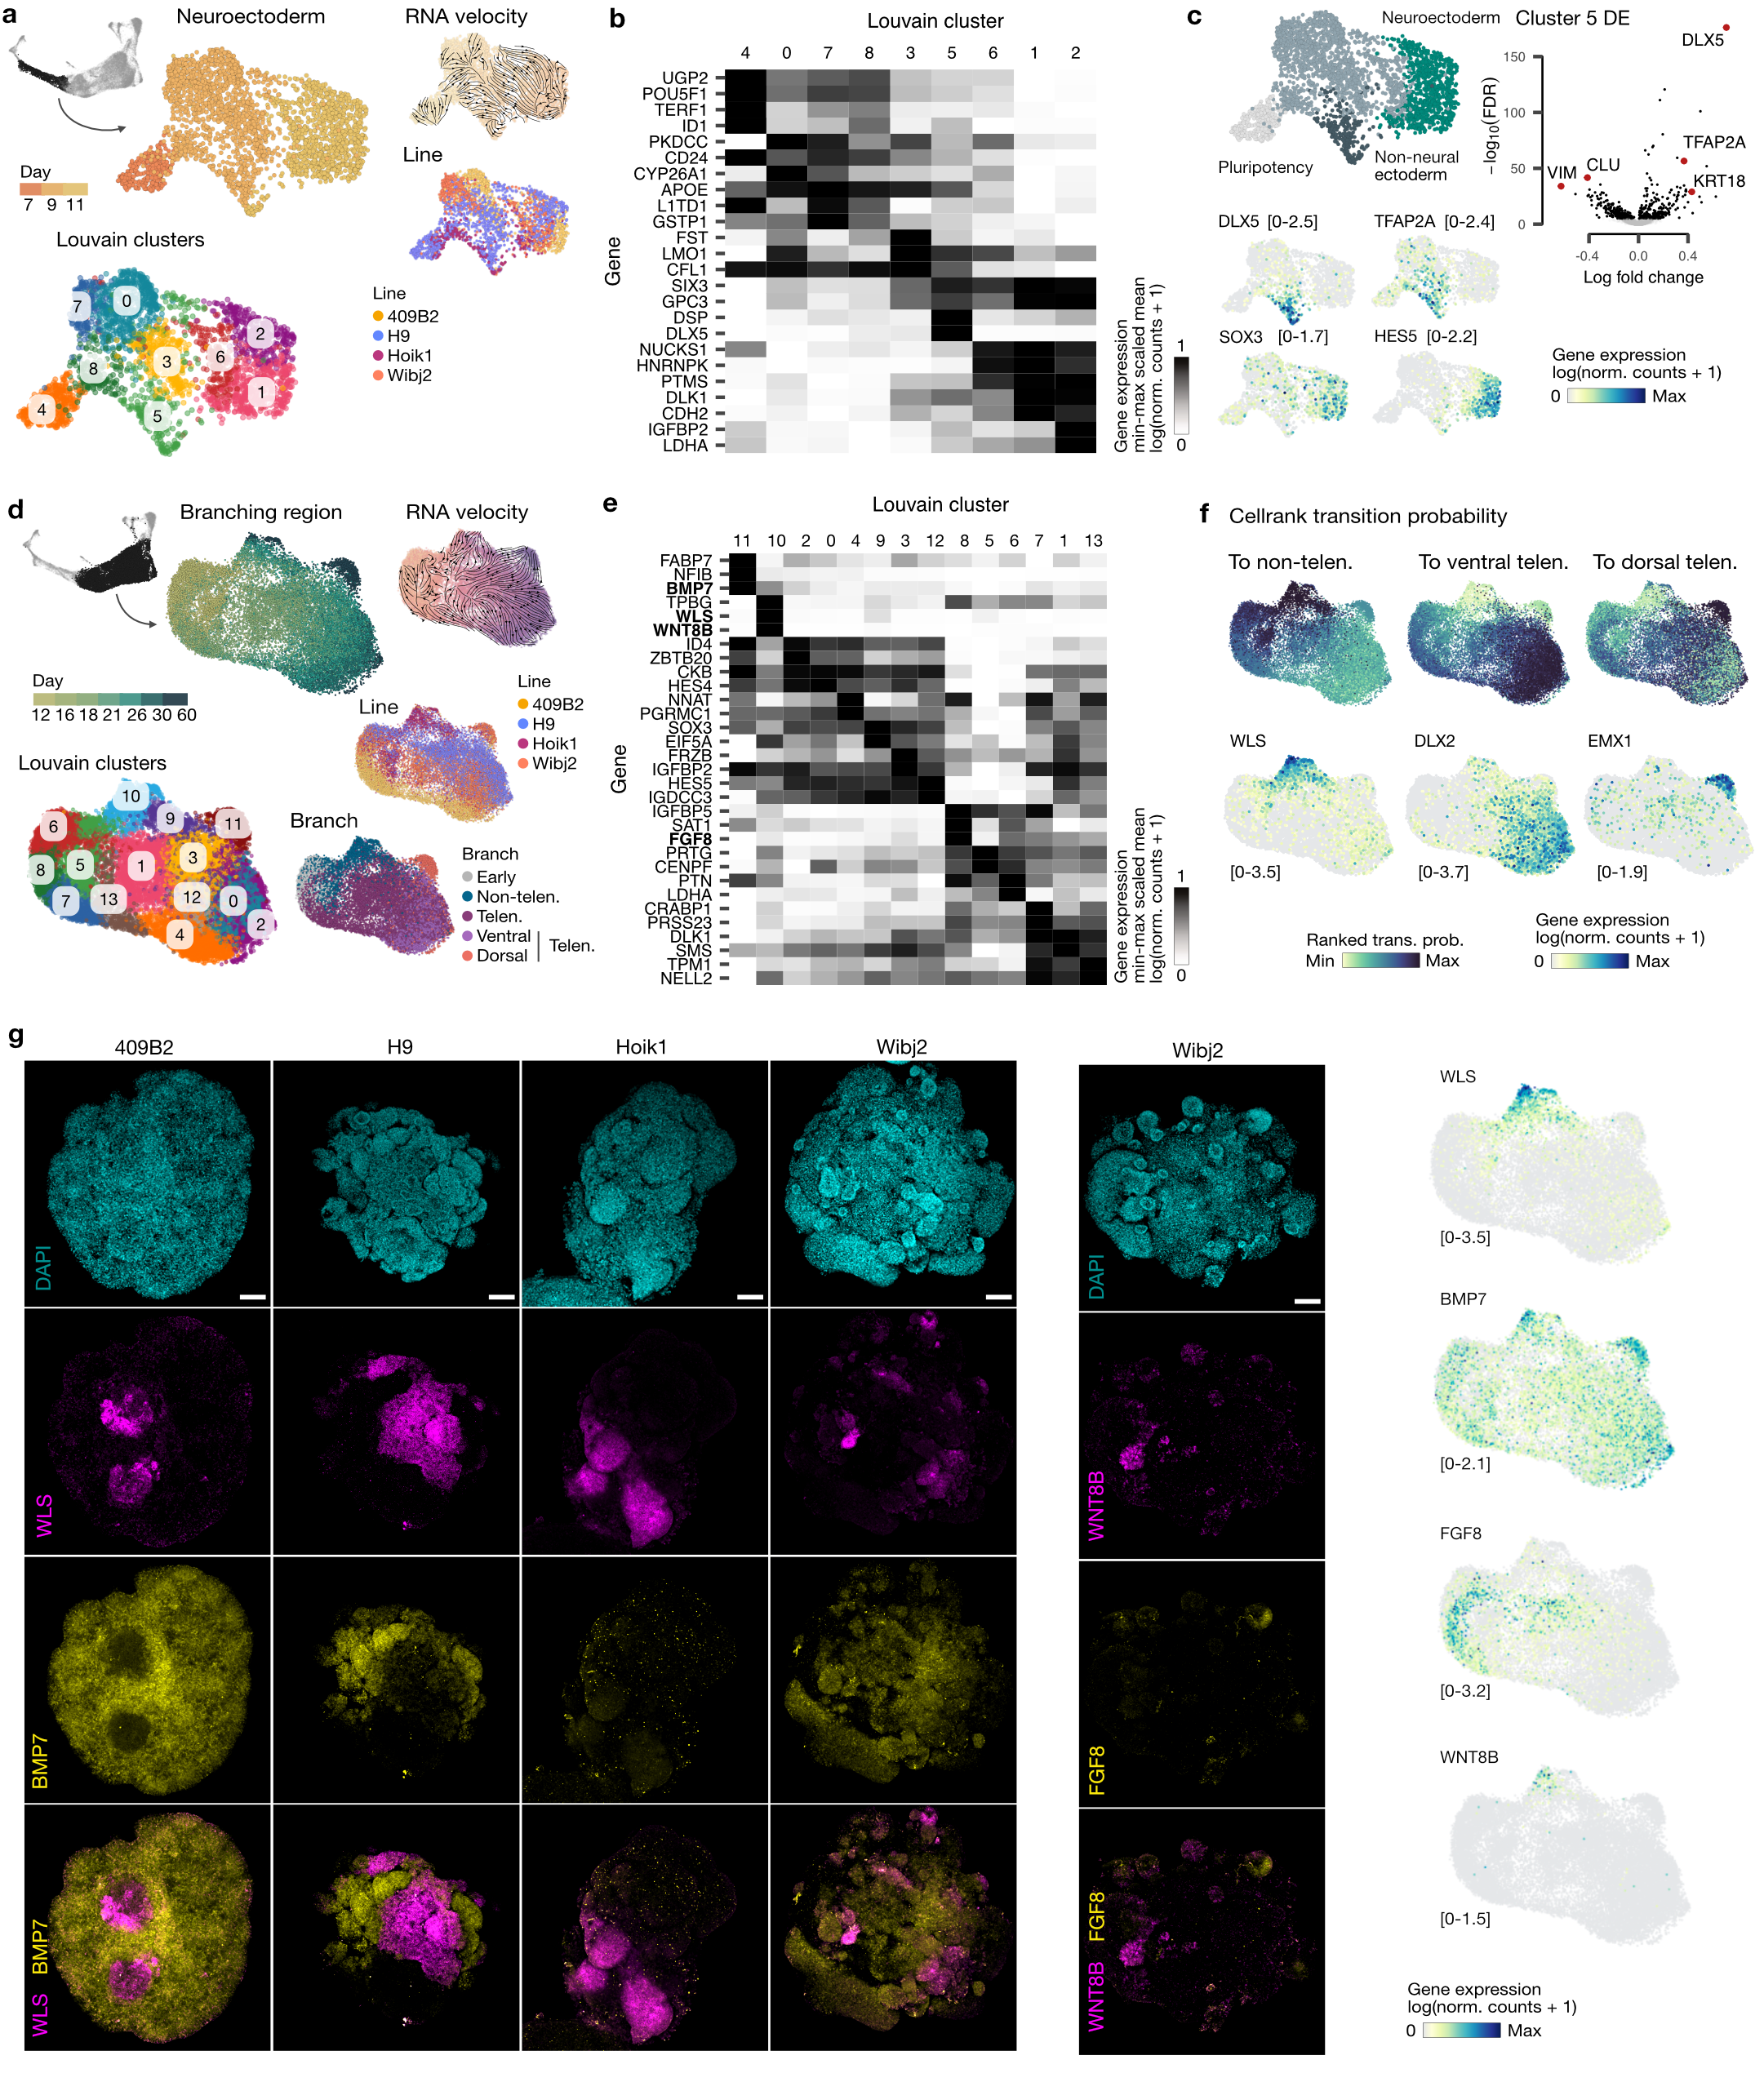
\includegraphics[width=\textwidth]{figures/pando/Figure_S2}
    \label{fig:regS2}
    \caption{\textbf{Heterogeneity analysis in different stages of organoid development.} a,d, UMAP embedding of a subset of the organoid trajectory surrounding neuroectoderm cells (a) and the branching window (d) colored by time point, velocity pseudotime, cell line, branch prediction and lovain clusters. b,e, Heatmap showing mean min-max scaled expression (log(transcript counts per 10k + 1)) of cluster markers. c, UMAP embedding colored by cluster identities, expression patterns of cluster markers. Volcano plot shows differentially expressed (DE) genes of cluster 5 relative to other clusters. f, UMAP embedding colored by rank-transformed CellRank transition probability to non-telencephalon, ventral telencephalon and dorsal telencephalon and colored by expression of selected transcription factors. g, Whole-mount HCR in situ hybridizations of day 18 organoids and UMAP embedding colored by expression of targets. Stainings were performed on 2-3 organoids per cell line and representative images were shown. Scale bar: 100 $\mu$m. The range of expression values is indicated for each feature plot.}
\end{figure}


\begin{figure}[h!]
    \centering
	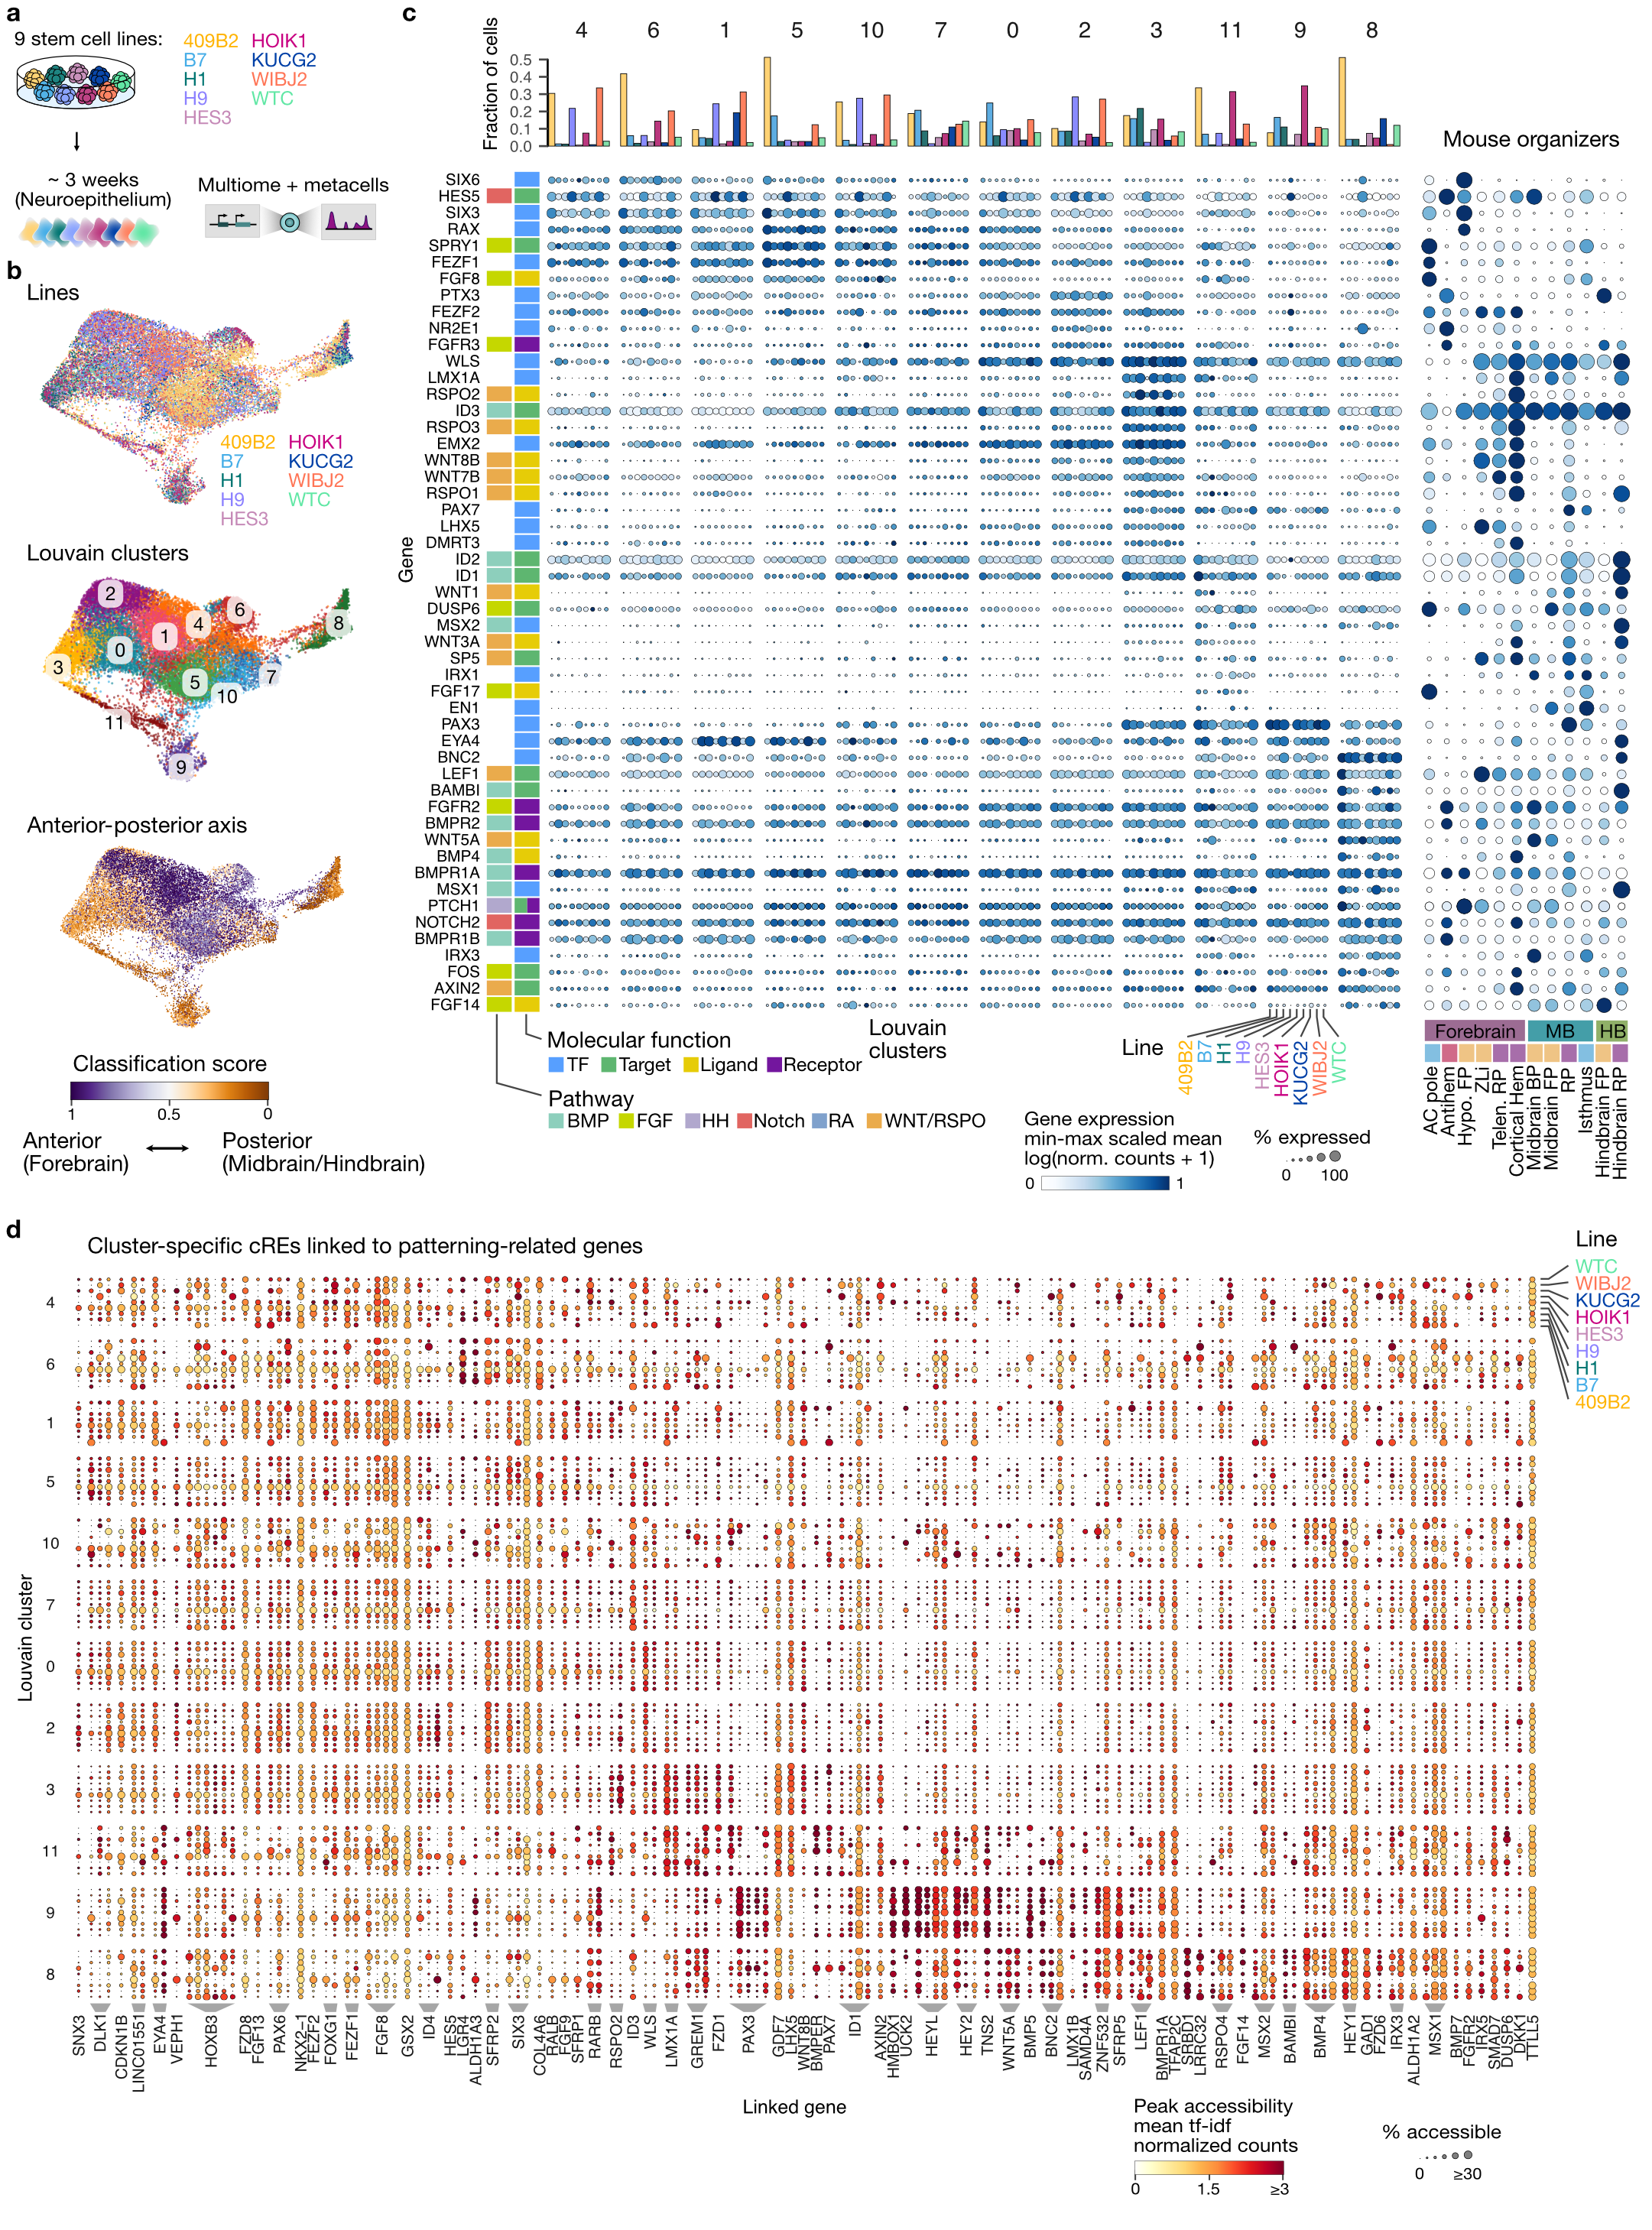
\includegraphics[width=\textwidth]{figures/pando/Figure_S3}
    \label{fig:regS3}
\end{figure}

\begin{figure}[t!]
    \centering
    \caption{\textbf{Signaling transcriptome and regulatory element landscape of the organoid neuroepithelium from 9 stem cell lines.} a, Schematic of the experimental setup. Multiome quantification was performed on organoids in the neuroepithelial stage (~3 weeks) from a total of 9 stem cell lines. The data was combined with the data from the same stage in the early time course. b, UMAP embedding colored by cell line, louvain clusters and anterior-posterior axis (forebrain versus non-forebrain) classification score. c, Bar plots (top) showing fraction of cells per cell line in each cluster. Dotplot (left) showing min-max scaled expression (log(transcript counts per 10k + 1))(color) and proportion of expressing cells (dot size) for transcription factors (TFs) and genes from different signaling pathways in clusters of 3 week old organoid data set split by cell line. All genes are annotated as TF, receptor, ligand, or TF target and if applicable, colored by the related signaling pathway. Dotplot (right) showing expression (color) and proportion of expressing cells (dot size) for the same genes of Figure S3.3d in mouse developing brain organizer cells of different brain regions (\cite{la_manno_molecular_2021}). d, Dot plot showing cluster-specific cis regulatory elements (CREs) linked to patterning genes split by different cell lines. Color and size indicate peak accessibility (if-idf normalized fragment counts) and proportion of expressing cells, respectively.}
\end{figure}

\clearpage

\begin{figure}[h!]
    \centering
	\includegraphics[width=\textwidth]{figures/pando/Figure_S4}
    \caption{\textbf{Trajectory reconstruction in the multi-omic developmental atlas.} a, Time course UMAP embedding colored by neuron types. b, Time course UMAP embedding colored by RNA velocity pseudotime. c, VoxHunt plots showing expression similarity of neuron subtypes in cerebral organoids to voxels in five example sections of the developing mouse brain (embryonic day 13.5),  as well as the structural annotation of the sections. d, UMAP embedding colored by ranked transition probabilities. e, Scatter plot showing mean transition probabilities as computed by CellRank versus velocity pseudotime. Each dot represents one high-resolution cluster. f, UMAP embedding of the integrated time course and graph embedding colored by gene expression (log(transcript counts per 10k +1)) (top) and gene activity (log(fragment counts per 10k +1))  (bottom) for selected marker genes. g, UMAP and graph representation colored by transcription factor motif enrichment z-score calculated with chromVAR (\cite{schep_chromvar_2017}) for selected motifs. The range of values is indicated for each feature plot.}
    \label{fig:regS4}
\end{figure}



\begin{figure}[h!]
    \centering
	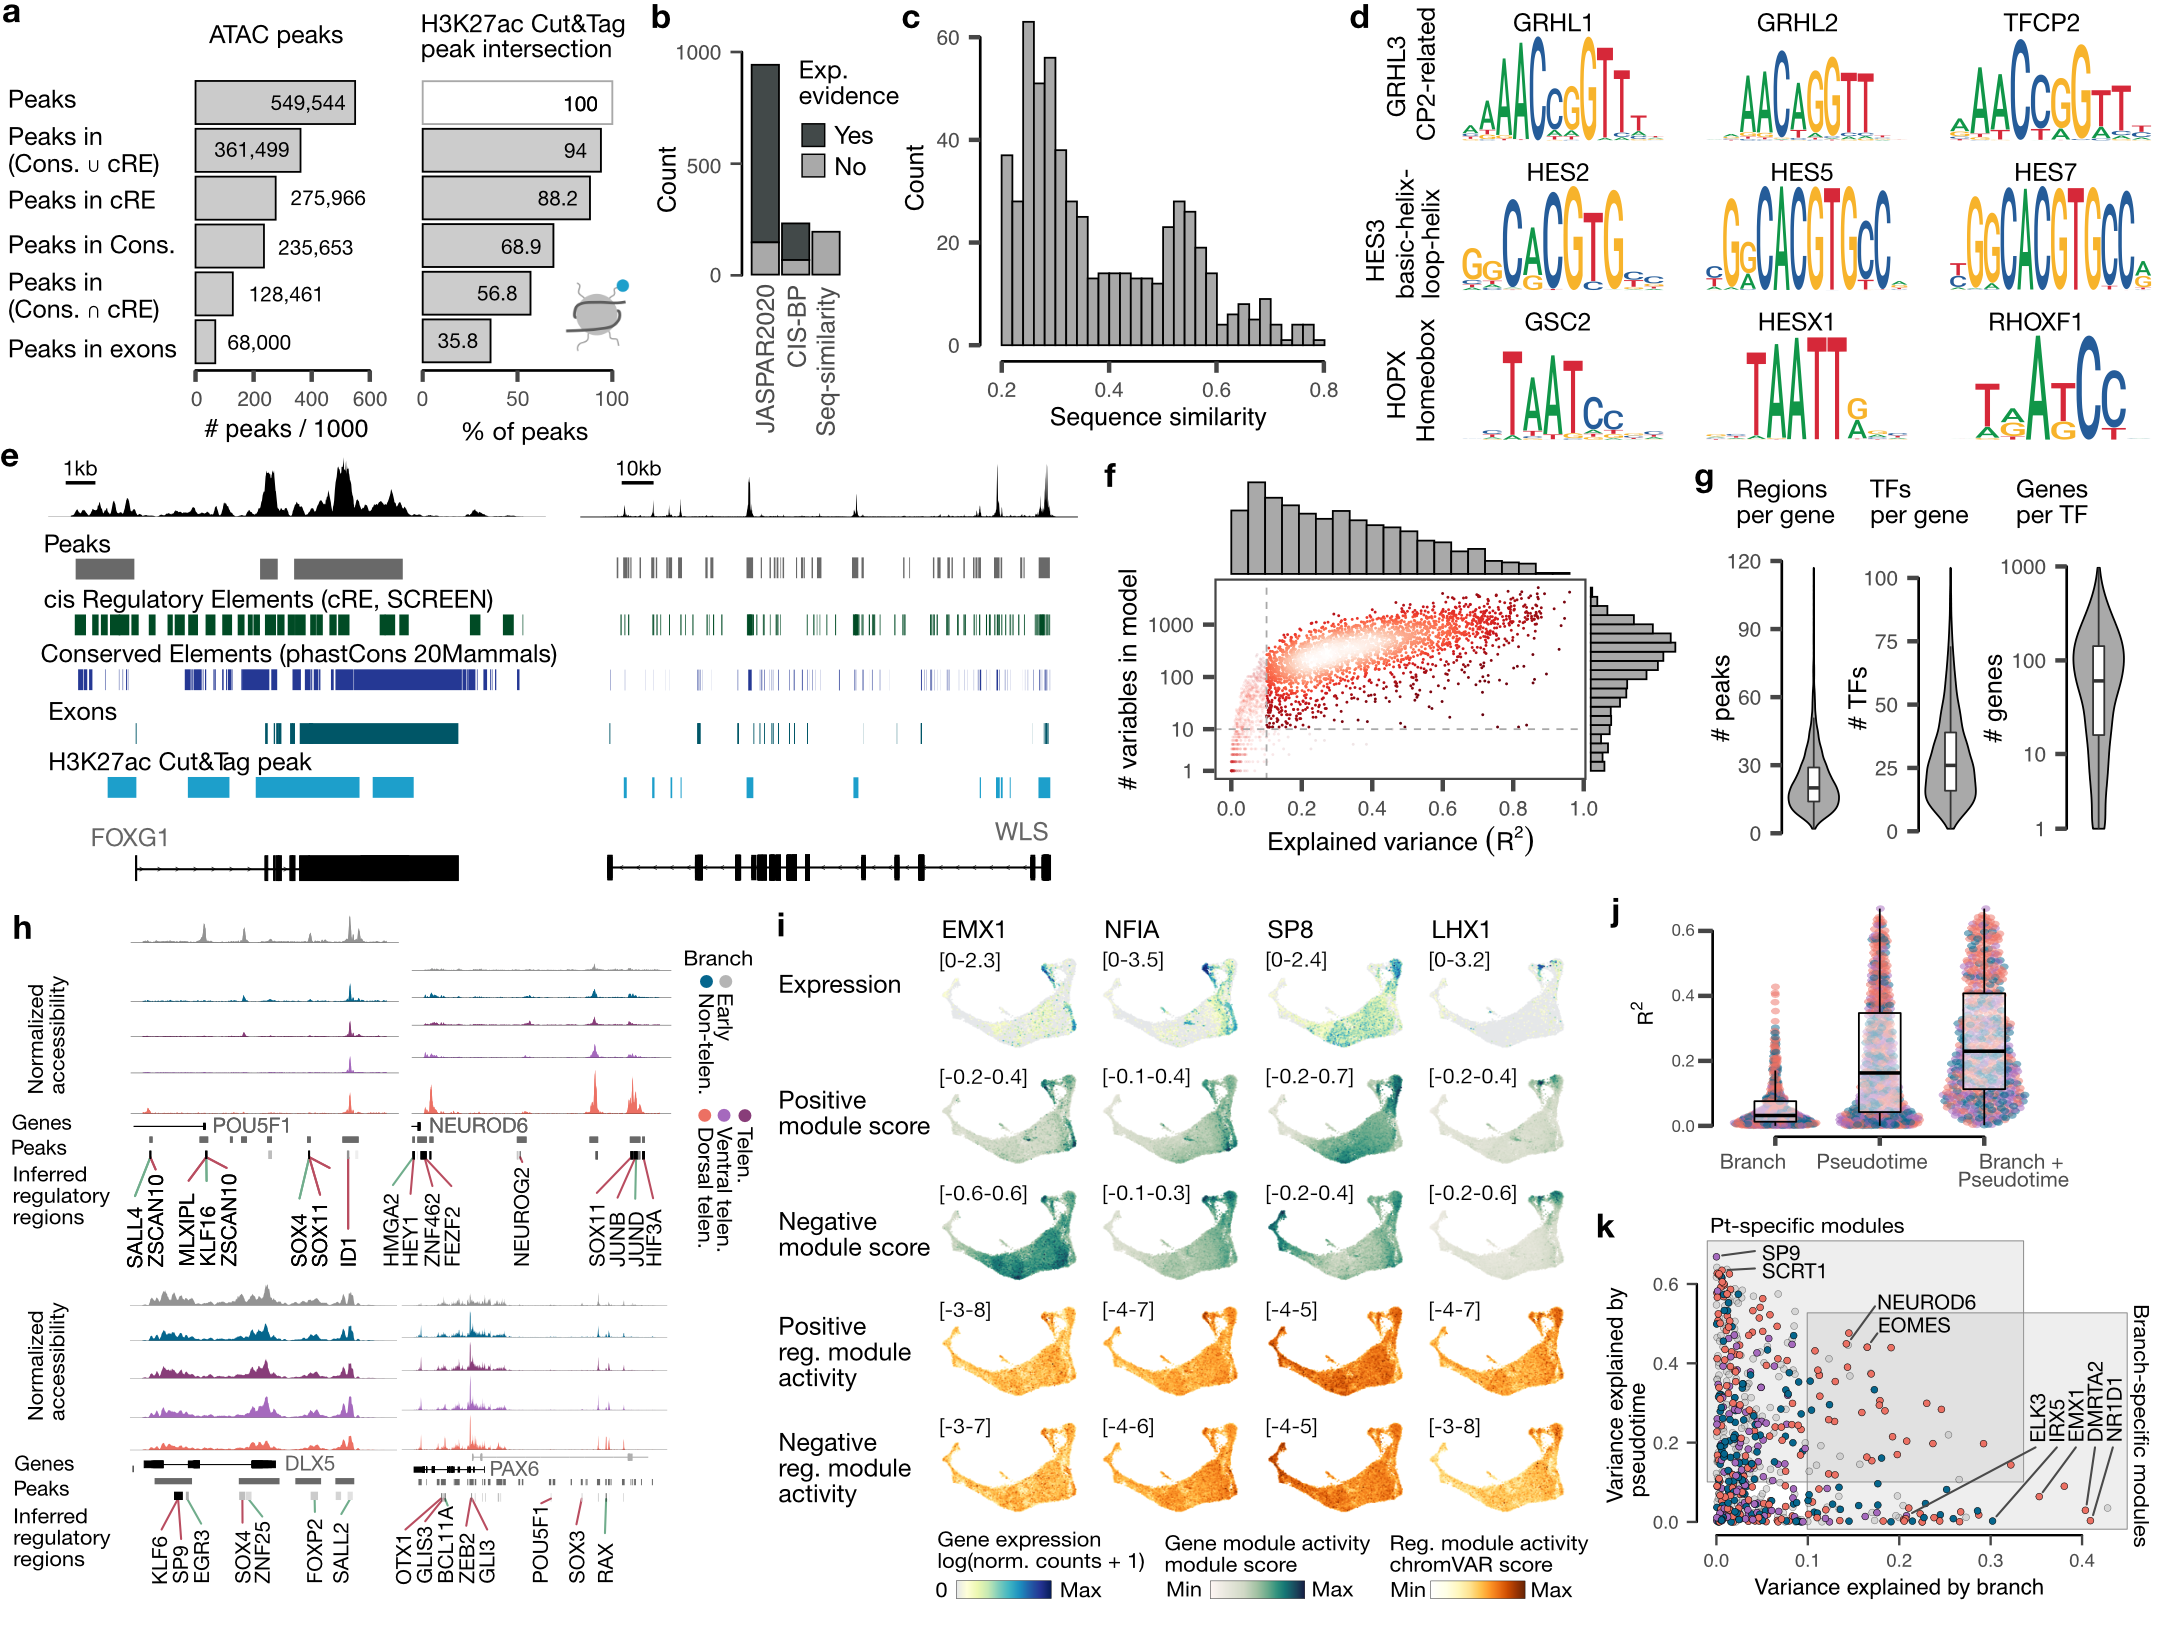
\includegraphics[width=\textwidth]{figures/pando/Figure_S5}
    \label{fig:regS5}
    \caption{\textbf{Gene regulatory network features of cerebral organoid development.} a, Numbers of chromatin access peaks and percentage of H3K27ac-marked peaks accessible at day 18-23 (>5\% detection) intersecting with non-protein coding conserved regions (Cons.), candidate cis regulatory regions (CRE), or exons (left). b, Representative loci showing chromatin access (top) overlaying peak, CRE, conserved elements, and exon coordinates. c, Barplot showing the number of motifs used in GRN construction from two curated databases (JASPAR, CIS-BP), and motifs assigned through amino acid sequence similarity. d, Examples of 3 TFs with no motif annotation that were assigned motifs based on sequence similarity. e, Loci for two exemplary genes (FOXG1, WLS) showing average chromatin access signal tracks, accessible peaks, CREs, conserved elements, exons and H3K27ac Cut\&Tag peaks. f, Scatter plot and histograms show explained variance (x) versus number of variables (y) of models for GRN construction. g, Violin plots show the distribution of peaks (left, n=2535 target genes) and TFs per gene (middle, n=2535 target genes), and number of genes per TF (right, n=720 TFs). h, Representative loci showing average chromatin access signal tracks at different developmental branches overlaying inferred transcription factor binding sites within regulatory regions. i, UMAP representation of time course colored by gene expression (log(transcript counts per 10k + 1)), gene module activity (module score calculated with Seurat) (rows), and regulatory module enrichment z-score (calculated with chromVAR) for representative TFs (columns). The range of values is indicated for each plot. j, Variation of module activity explained by branch, pseudotime, or branch and pseudotime (n=720 TF modules). Box plot center lines represent the median, boxes indicate 25\%-75\% interquantile range and whiskers 1.5 * interquantile range. k, Branch and pseudotime specific TF modules. Colors represent the branch with highest average module activity. TFs without experimentally validated motif are shown in gray. }
\end{figure}


\begin{figure}[h!]
    \centering
	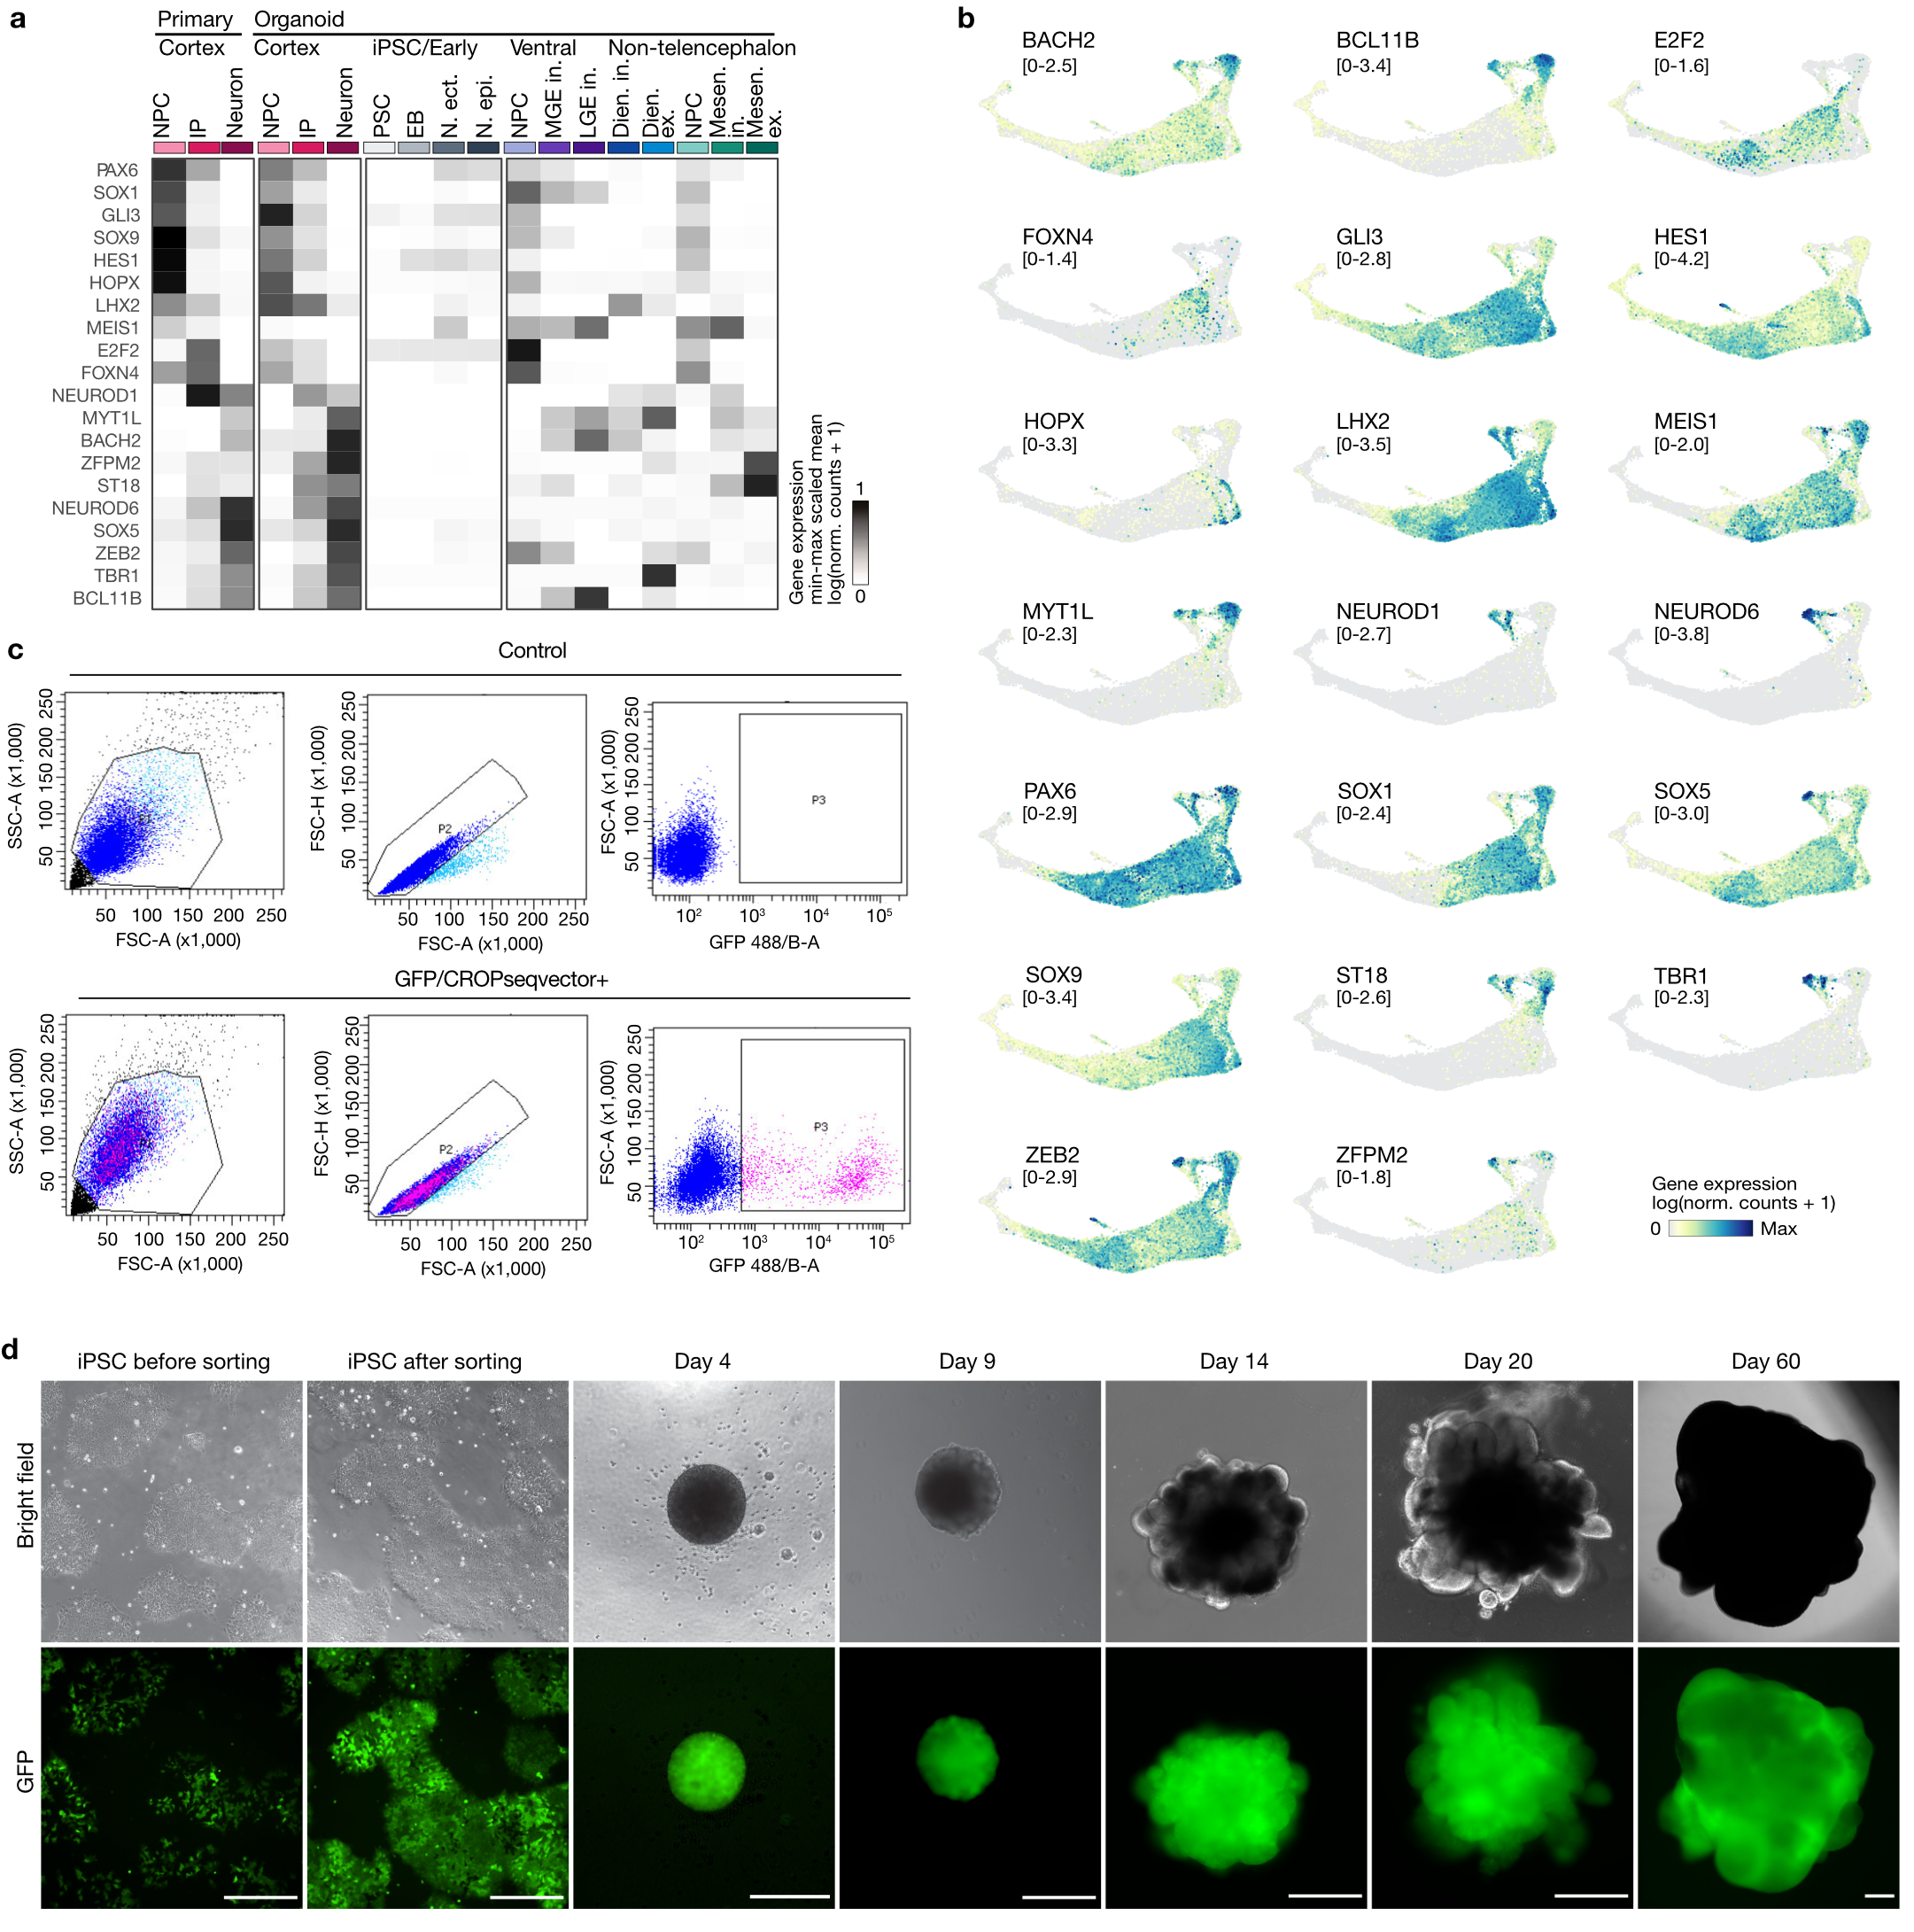
\includegraphics[width=\textwidth]{figures/pando/Figure_S6}
    \label{fig:regS6}
    \caption{\textbf{Target selection and experimental details for the single-cell \textit{in organoid} perturbation experiment.} a, Min-max scaled mean expression (log(transcript counts per 10k + 1)) of genes targeted in the single-cell genomic perturbation experiment in neuronal progenitors (NP), intermediate progenitors (IP) and neurons in the primary human and organoid developing cortex, as well as in induced pluripotent stem cells (IPSC), the embryoid body (EB), ventral telencephalic NPCs, inhibitory neurons of the medial ganglionic eminence (MGE in.), lateral ganglionic eminence (LGE in.), non-telencephalic NPCs, diencephalic excitatory neurons (Dien. ex.) and inhibitory neurons (Dien. in.) and mesencephalic excitatory neurons (Mesen. ex.) and inhibitory neurons (Mesen. in.). b, UMAP embedding colored by the expression of all targeted genes. The range of expression values is indicated for each feature plot. c, Exemplary Fluorescence-activated cell sorting plots of the sorting scheme used to isolate CROP-seq vector positive induced pluripotent stem cells (iPSCs). d, Phase contrast and CROP-seq vector positive (GFP) imaging during cerebral organoid development. Images are representative for 48 imaged organoids. Scale Bar is 500 $\mu$m.}
\end{figure}


\begin{figure}[h!]
    \centering
	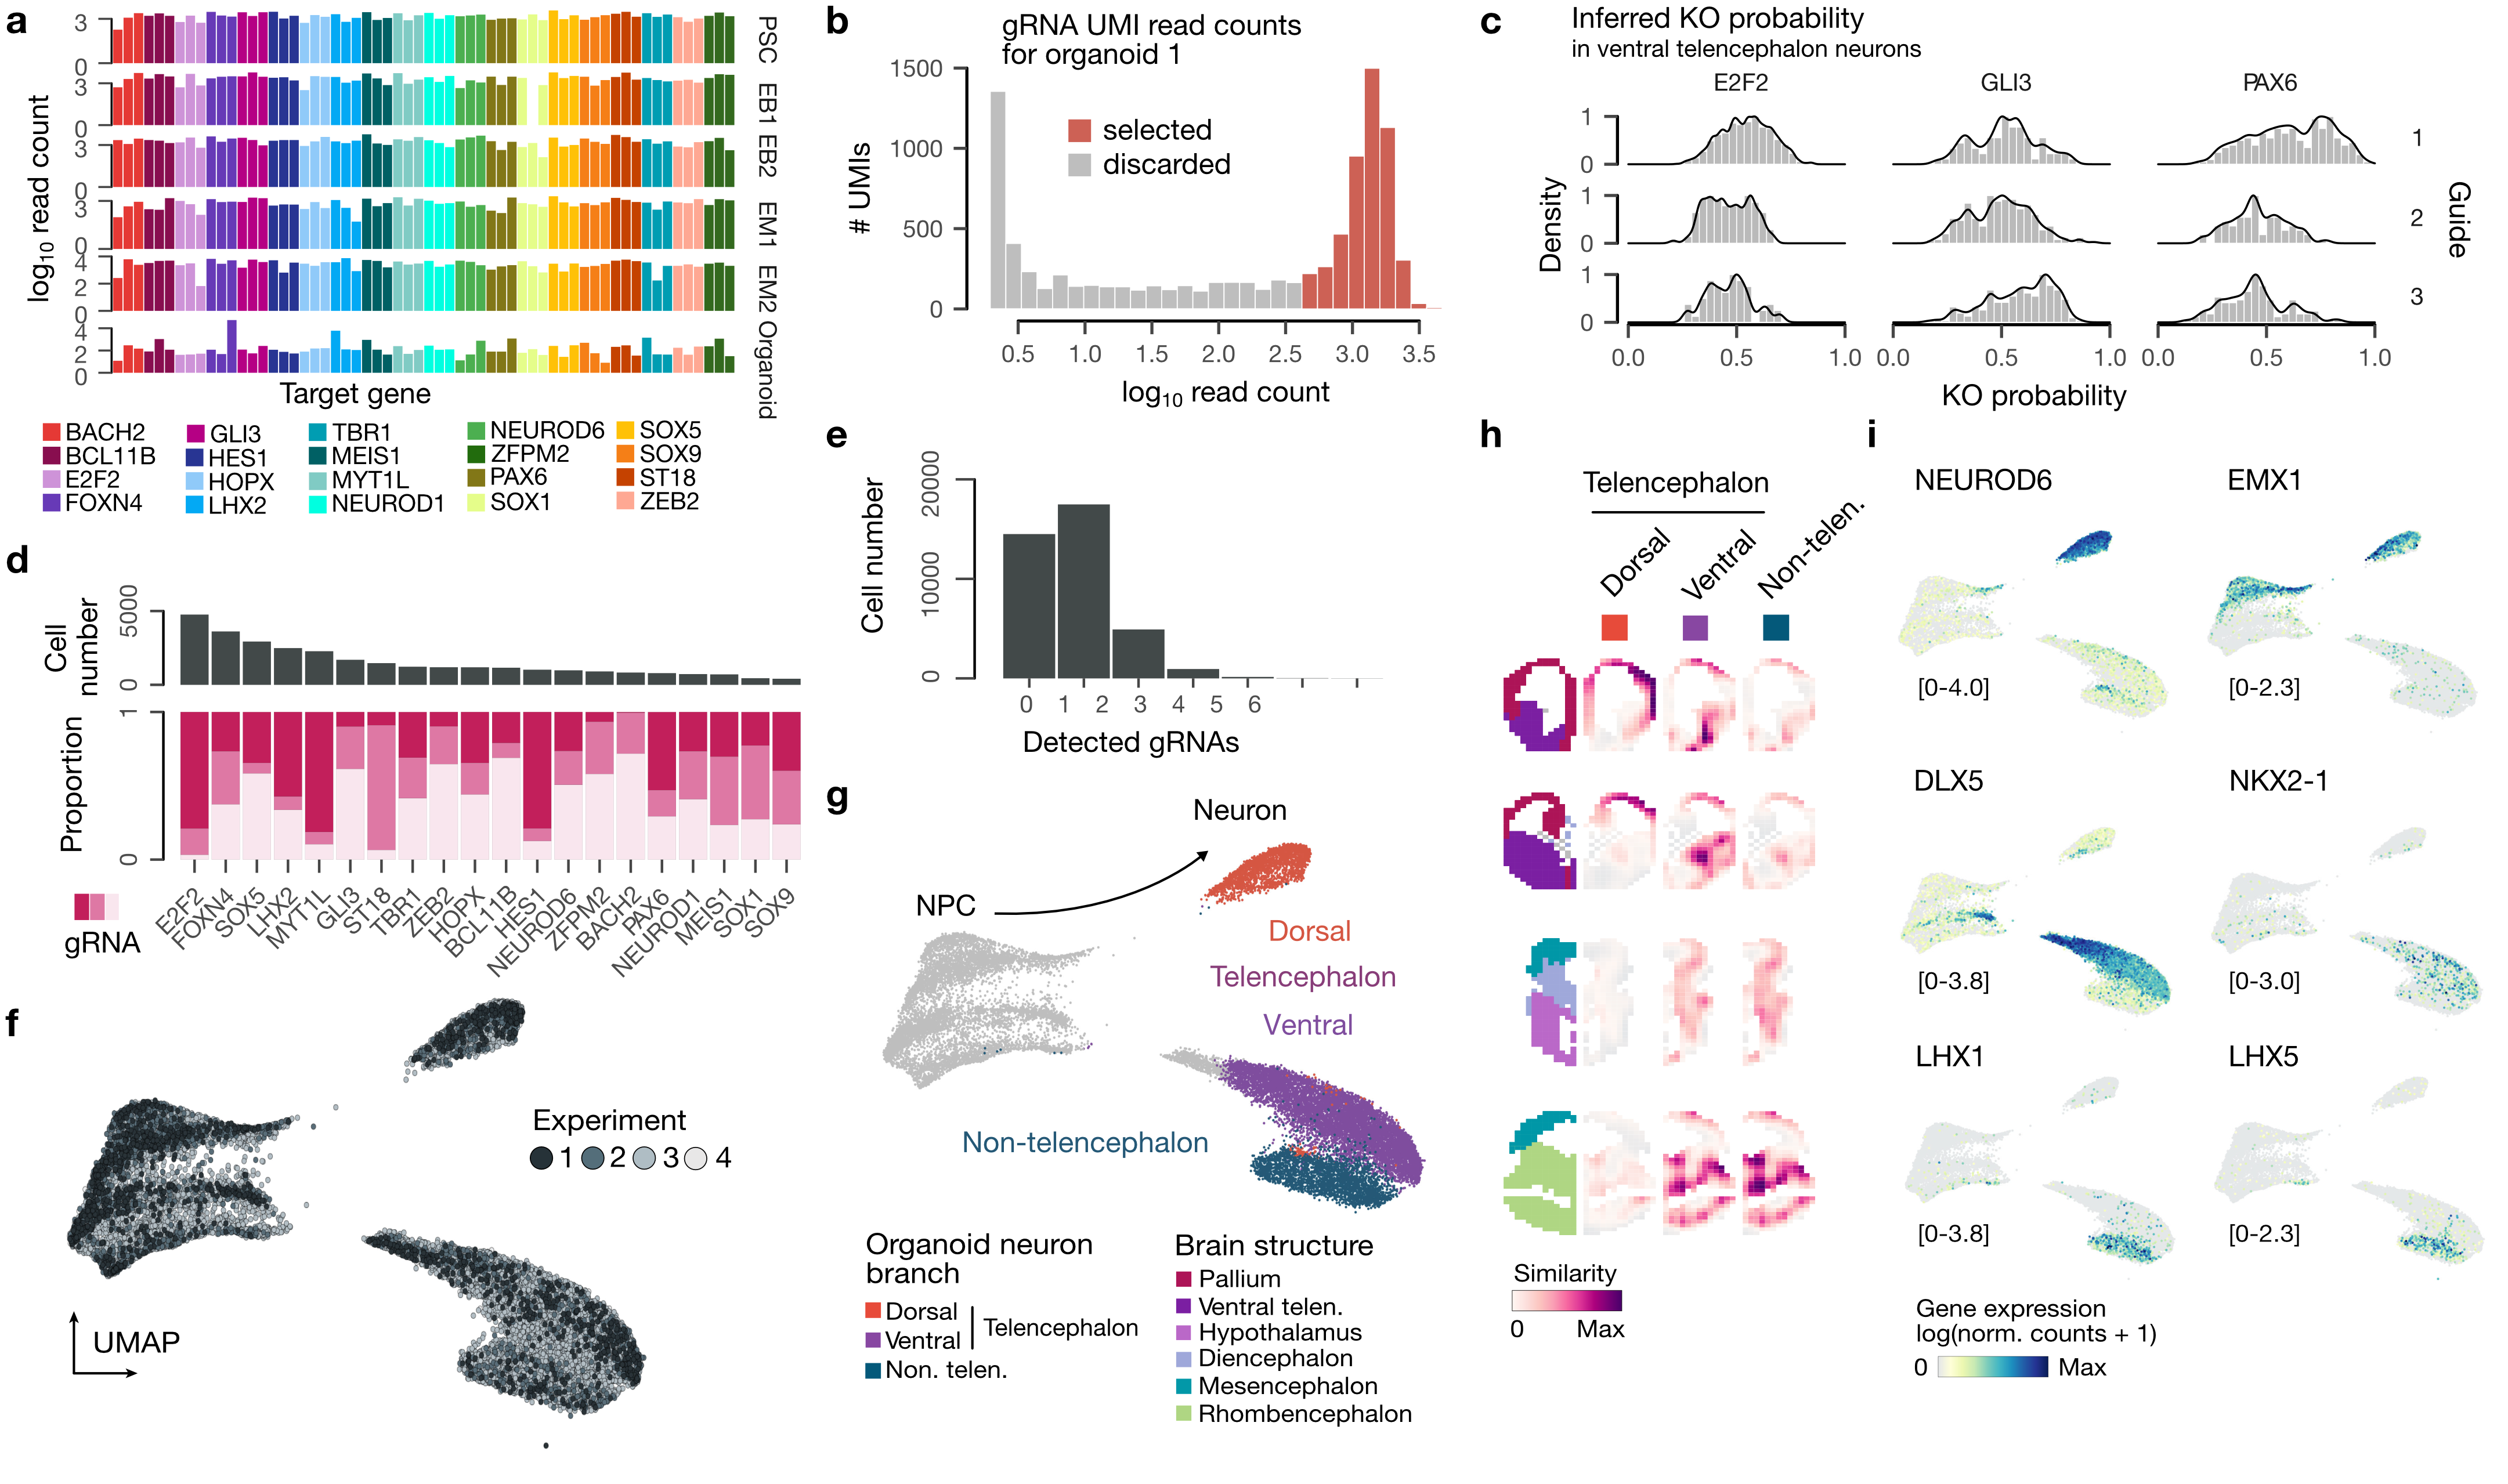
\includegraphics[width=\textwidth]{figures/pando/Figure_S7}
    \label{fig:regS7}
    \caption{\textbf{Guide detection and cell type annotation in the single-cell perturbation experiment in organoids.} a, Barplot showing number of cells with detected guide RNA (gRNA) for each targeted gene and stacked barplot showing the distribution of the different gRNAs targeting the same gene. b, Histogram showing the distribution of read counts for gRNA UMIs after amplicon sequencing for one organoid. UMIs marked in red were selected for downstream analyses. c, Density histograms showing the distribution of inferred KO probabilities for gRNAs of 3 different target genes. d, Barplot showing cell number and proportion of gRNAs for all target genes. e, Barplot showing the number of guides detected in sequenced cells. f, UMAP embedding with cells colored based on experiment. g, UMAP embedding colored by annotated neuron subtypes. h, VoxHunt plots showing expression similarity of neuron subtypes in cerebral organoids to voxels in five example sections of the developing mouse brain (embryonic day 13.5), as well as the structural annotation of the sections (left). i, UMAP embedding colored by expression (log(transcript counts per 10k + 1)) of non-telencephalic (top), ventral (middle) and dorsal (bottom) neuron markers. The range of expression values is indicated for each feature plot.}
\end{figure}




\begin{figure}[h!]
    \centering
	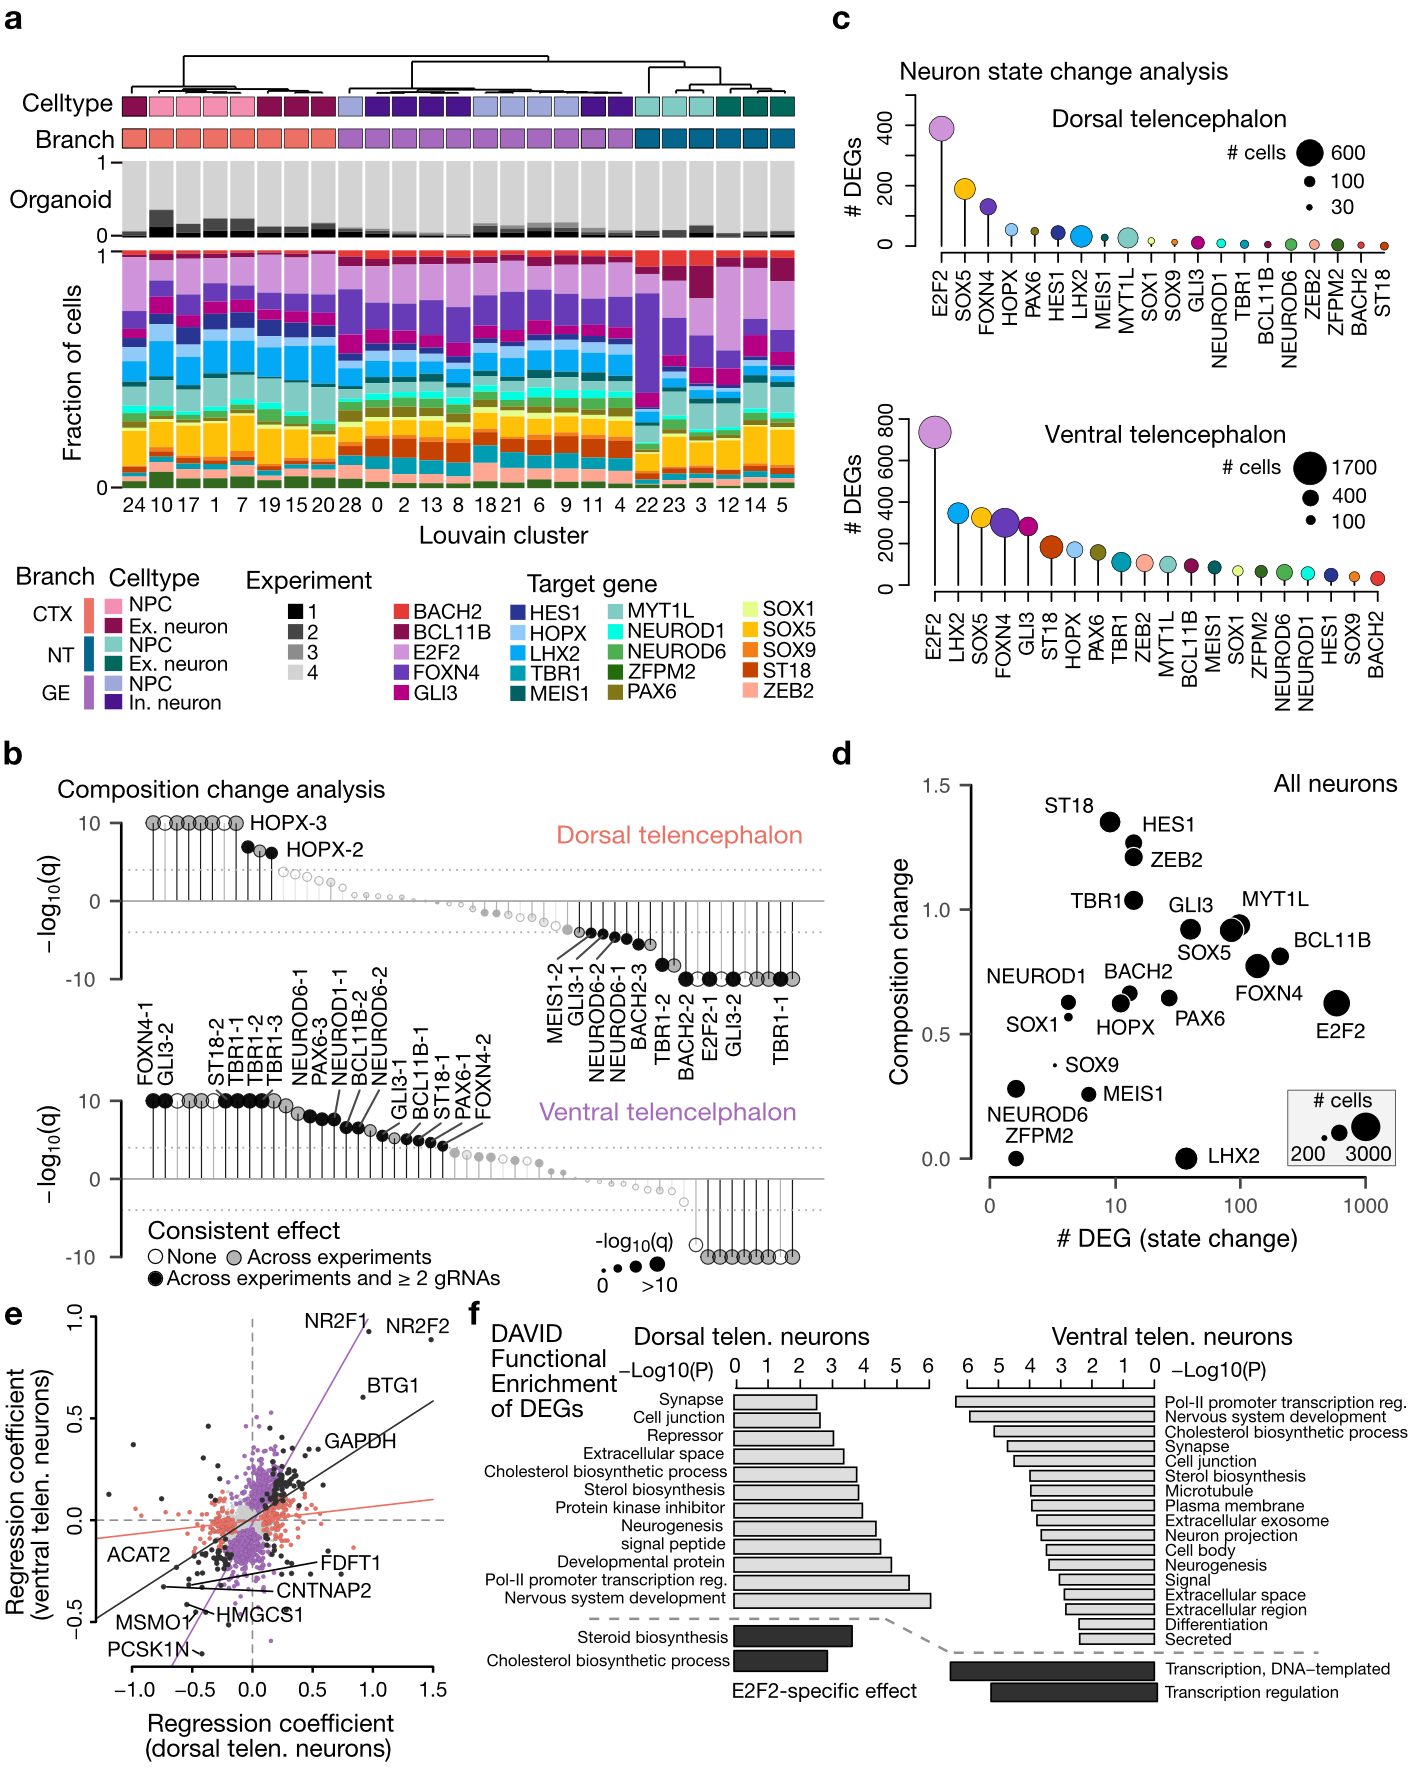
\includegraphics[width=\textwidth]{figures/pando/Figure_S8}
    \label{fig:regS8}
\end{figure}

\begin{figure}[h!]
    \centering
    \caption{\textbf{Composition and expression changes after CRISPR-Cas9 perturbations in mosaic brain organoids.} a, Hierarchical clustering of Louvain clusters based on the composition of gRNAs targeting different genes. Cell type and branch annotations are shown as side bars. Compositions of organoids and composition of cells with gRNAs targeting different genes are shown below as stacked bar plots. b, Lollipop plot showing the impact of each gRNA on cell type abundance in dorsal and ventral telencephalic neurons. c, Lollipop plots showing number of differentially expressed genes (DEG) for targeted genes in the dorsal and ventral telencephalic neurons. d, Differential gene expression analysis was performed to identify potential effects on cell state. Plot shows the effect of cell composition change and the number of differentially expressed genes (DEGs). P-values were derived using an F-test based ANCOVA.  e, Scatter plot shows expression changes between neurons with E2F2 targeting gRNAs and other neurons in dorsal (x-axis) and ventral (y-axis) telencephalic neurons, with each dot representing one gene. Colors of dots represent the neuron types where differential expression is detected. Lines show the correlation of expression changes in the two neuron types, with DE genes in both types and DE genes in only one type shown separately. f, Examples of functional enrichment for E2F2 DEGs in dorsal and ventral neurons with DAVID. Gray bars show enriched terms of all E2F2 DEGs, and dark bars show enriched terms of DEGs with E2F2-specific effects.}
\end{figure}

\clearpage


\begin{figure}[h!]
    \centering
	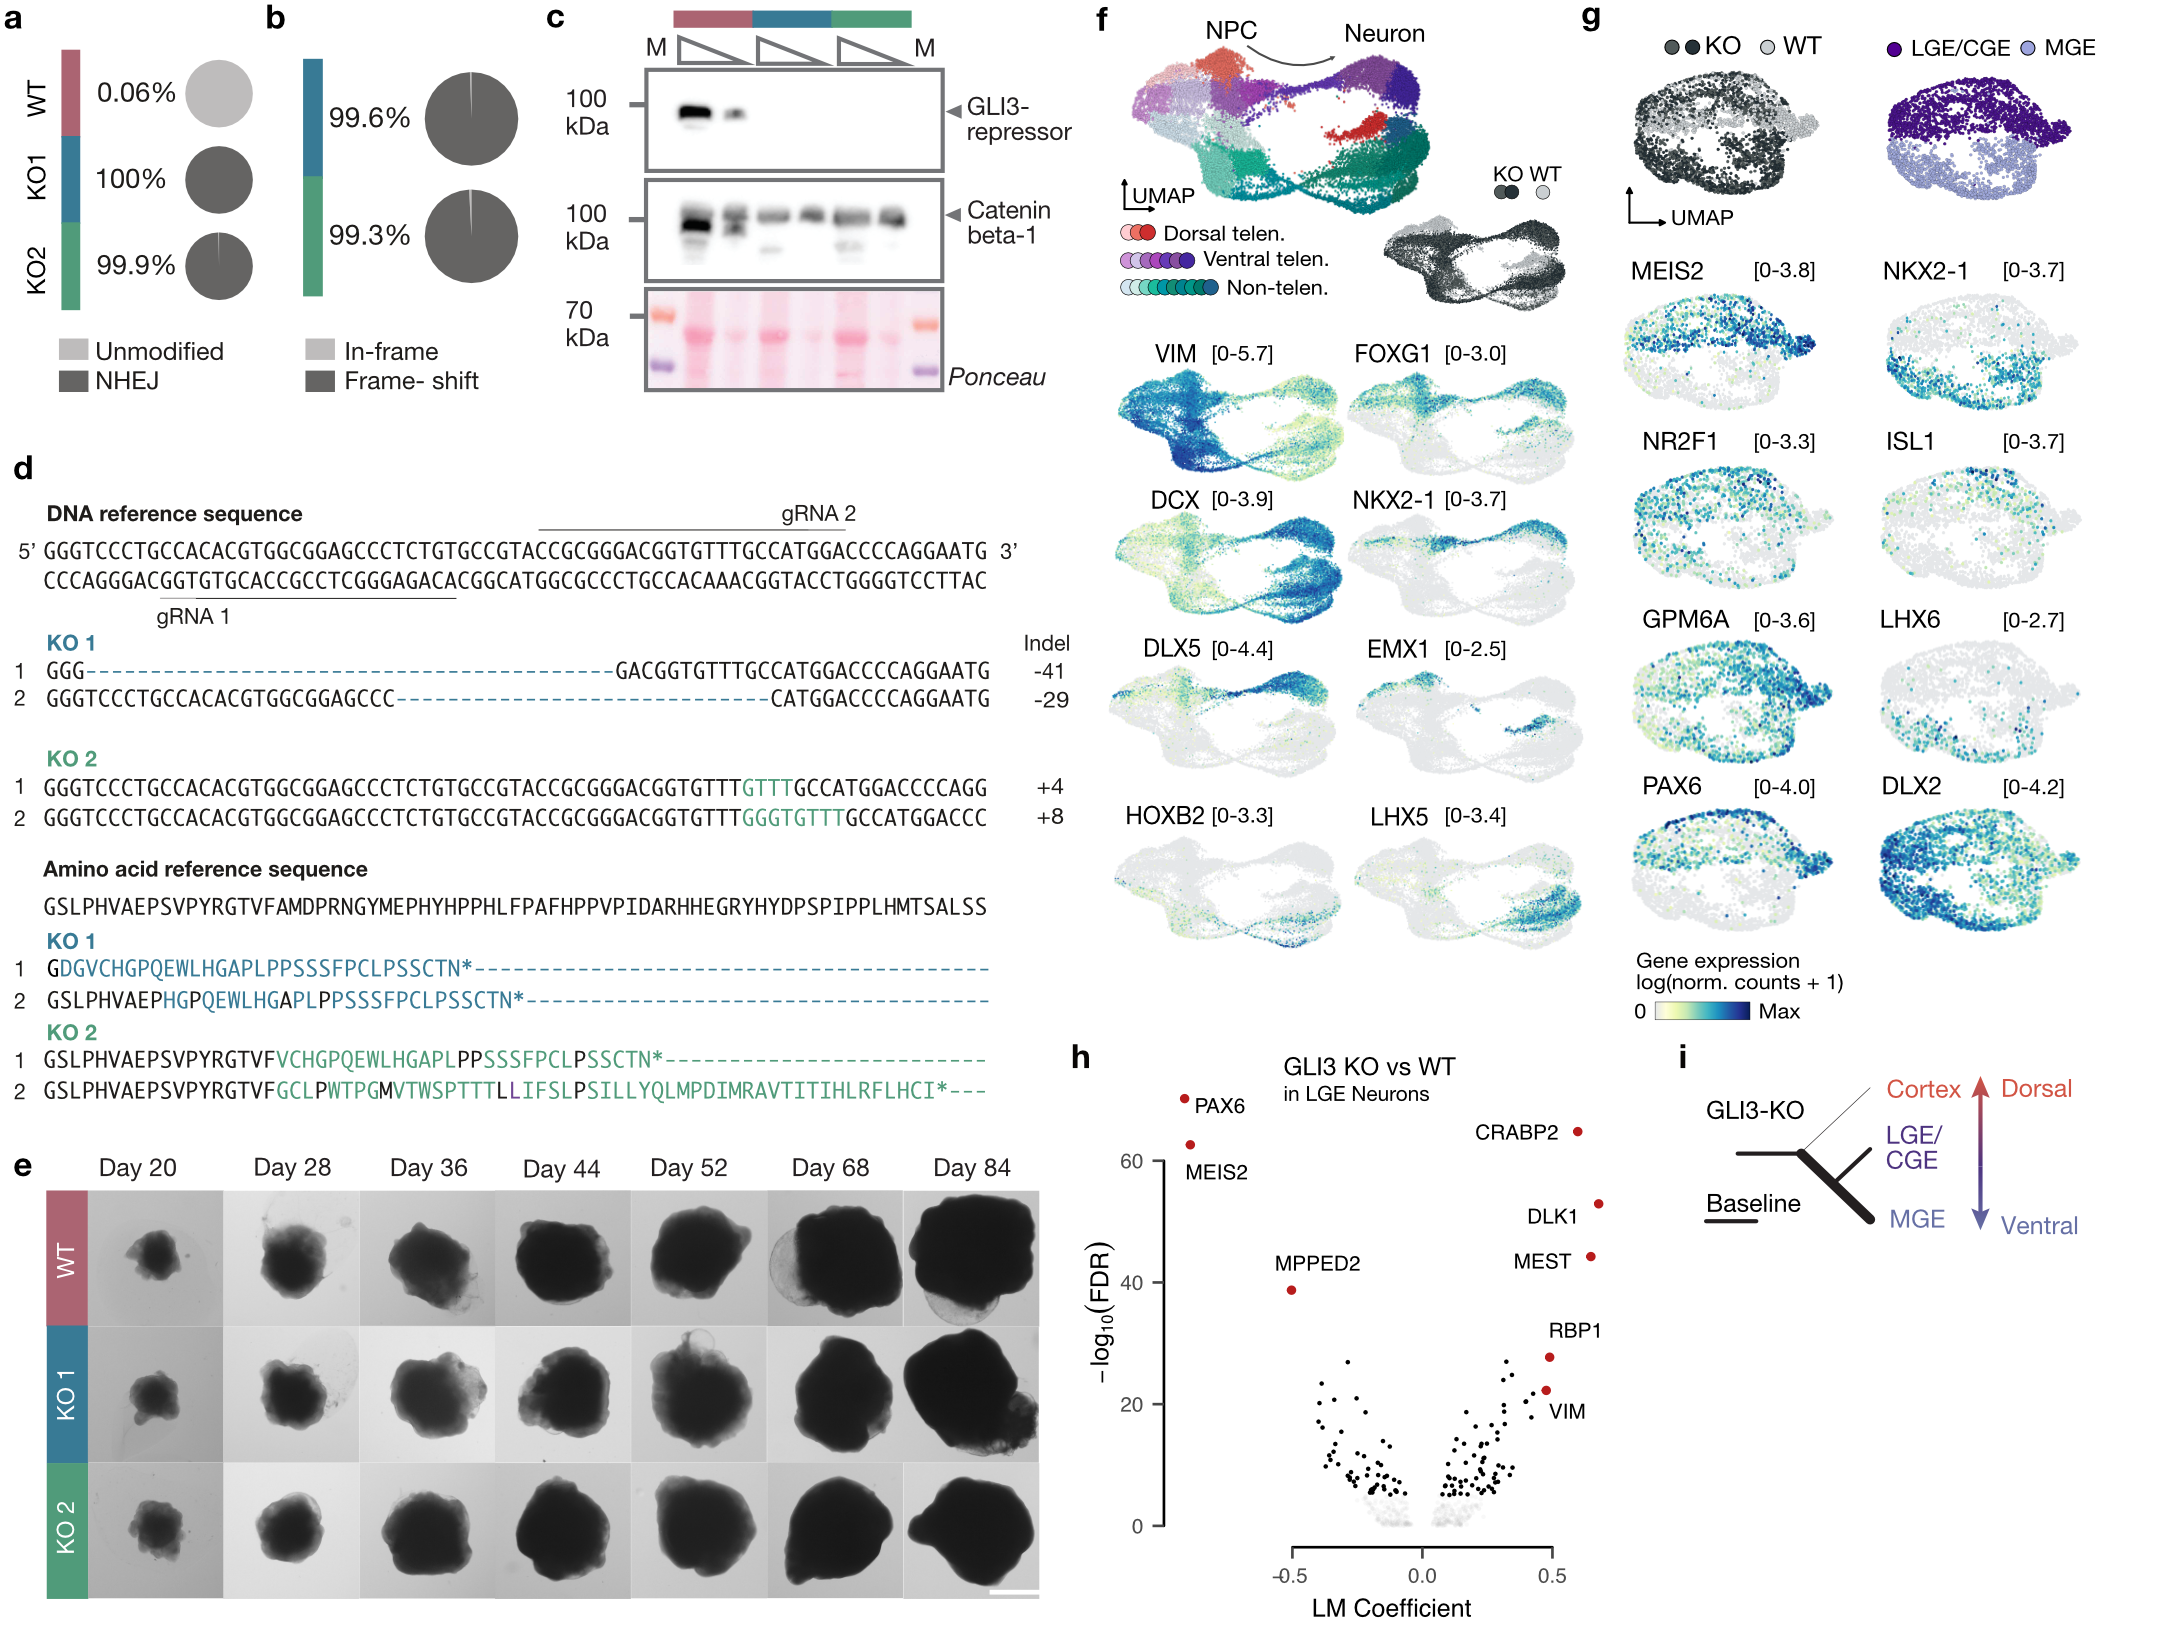
\includegraphics[width=\textwidth]{figures/pando/Figure_S9}
    \label{fig:regS9}
    \caption{\textbf{Characterization of GLI3 knock-out organoids.} Quantification of editing frequency as determined by the percentage and number of sequence reads showing unmodified and modified alleles for the control and both KO cell lines. b, Frequency of frameshift of coding sequence reads as a result of the modifications seen in both KO lines. c, Western blot showing expression of Gli3-repressor (83kDA) in the control cell line. Catenin beta-1 and Ponceau were used as loading control. For western blot source data, see Supplementary Data Figure 3.1. d, Sequences of the coding strand of the different indels of the different KO lines. The reference sequence is corresponding with the control line. The position of the gRNAs with the protospacer adjacent motif (PAM)-sequence is depicted above and underneath the sequence. Reference protein sequence with the protein sequences of each KO line of the altered protein sequences caused by the frame-shift. e, Brightfield images of cerebral organoid development with control and both KO cell lines. Images are representative for 16 imaged organoids per line. Scale bar is 2 mm. f, UMAP embedding showing trajectories from neural progenitor cells (NPCs) to neurons colored by different clusters assigned to branches (dorsal, ventral, and non-telencephalon), with inset colored by genetic condition and feature plots colored by expression (log(transcript counts per 10k + 1)) of cell type markers. g, UMAP embedding of ventral telencephalic GLI3 KO neurons showing medial ganglionic eminence (MGE) and lateral/caudal ganglionic eminence (LGE/CGE) neuronal populations (top). Feature plots show selected marker gene expression on the UMAP embedding. The range of expression values is indicated for each feature plot. h, Volcano plot showing differential expression analysis in LGE neurons for GLI3 WT versus KO cells. i, Schematic of observed effect of GLI3 loss of function on dorsoventral telencephalic fate decisions. }
\end{figure}


\begin{figure}[h!]
    \centering
	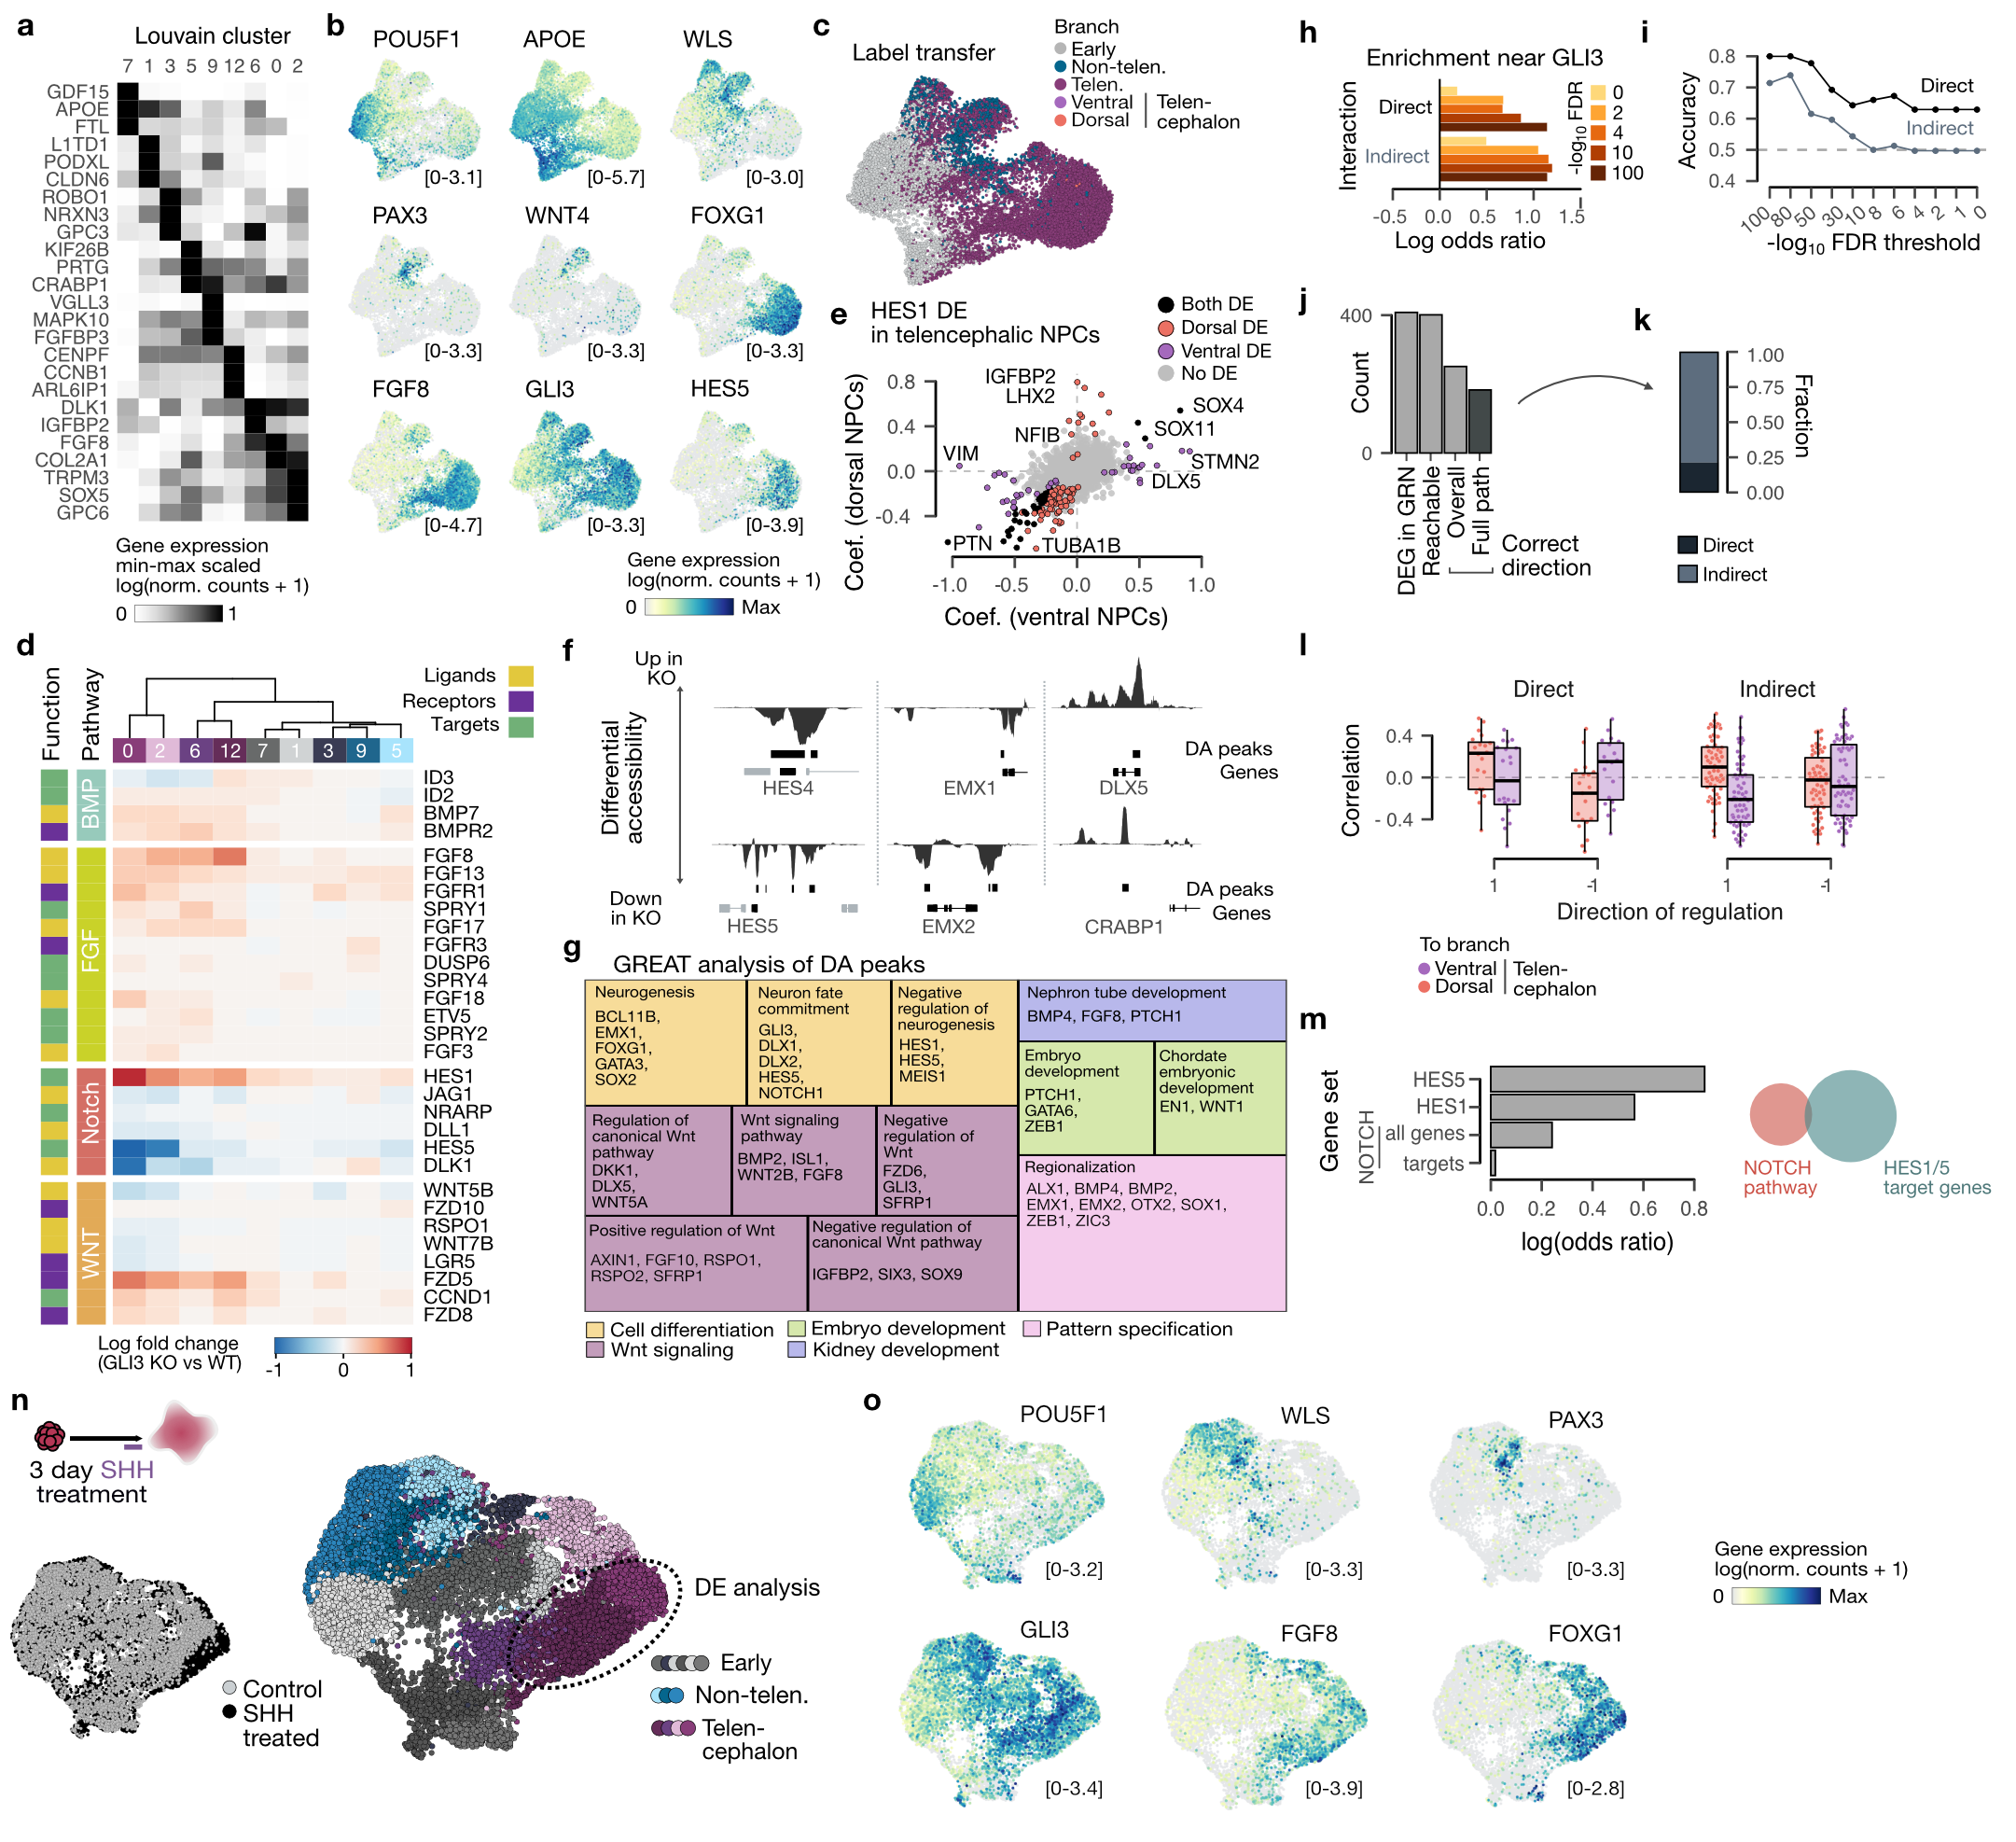
\includegraphics[width=\textwidth]{figures/pando/Figure_S10}
    \label{fig:regS10}
    \caption{\textbf{GLI3 KO induced changes in telencephalic progenitors in cerebral organoids.} a, Heatmap showing min-max scaled expression (log(transcript counts per 10k +1)) of marker genes for unbiased Louvain clusters. b,  UMAP colored by the expression of selected marker genes. The range of values is indicated for each plot. c, UMAP embedding colored by branch labels predicted by label transfer from the organoid time course. d, Heatmap showing DE associated with signaling pathways. e, Scatter plot showing DE in neural progenitor cells (NPCs) upon HES1 perturbation in the mosaic perturbation experiment. f, Signal tracks showing differentially accessible (DA) peaks in cluster 0 and 2. g, GREAT enrichment analysis of DA peaks in cluster 0 and 2, with box area proportional to FDR. Representative genes are shown. h, Enrichment of DE genes in the neighborhood of GLI3 in the GRN. i, Accuracy of GRN predicted directionality of GLI3 effect at different false discovery rate (FDR) thresholds. j, Barplot showing the number of all DE genes in the GRN (DEG in GRN), all DE genes reachable from GLI3 in the graph (Reachable), DE genes where the GRN was consistent with the DE result (Overall) and DE genes for which all subpaths from GLI3 were consistent with the DE result (Full path). k, Barplot showing the fraction of DE genes directly and indirectly regulated by GLI3. l, Boxplot showing the spearman correlation of directly (n=39) and indirectly (n=126) regulated DE genes with transition probabilities ventral and dorsal branched. The center line represents the median, boxes indicate 25\%-75\% interquantile range and whiskers 1.5 * interquantile range. m, Barplot showing the enrichment of gene sets (HES1/5 target genes, NOTCH components) among telencephalic DE genes. n, UMAP embedding showing annotation of multiome SHH experiment. o, UMAP colored by the expression of selected marker genes.}
\end{figure}

\clearpage

\topparagraph{Supplementary Data}

\noindent
All supplementary data items can be obtained from polybox with the following link: \\ \href{https://polybox.ethz.ch/index.php/s/5ZbTkjaiCl1XUvr}{https://polybox.ethz.ch/index.php/s/5ZbTkjaiCl1XUvr} 

\vspace{0.5cm}
\noindent
{\normalfont\footnotesize\sffamily\textbf{Supplementary Data Figure 3.3.1 | Raw data western blots.} Red boxes indicate cropped areas shown in Figure S3.9.} 

\vspace{0.25cm}
\noindent
{\normalfont\footnotesize\sffamily\textbf{Supplementary Table 3.1 | Overview of single-cell genomic experiments.}}

\vspace{0.25cm}
\noindent
{\normalfont\footnotesize\sffamily\textbf{Supplementary Table 3.2 | Feature sets used for integration and GRN inference.}}

\vspace{0.25cm}
\noindent
{\normalfont\footnotesize\sffamily\textbf{Supplementary Table 3.3 | Stage-specific features.}}

\vspace{0.25cm}
\noindent
{\normalfont\footnotesize\sffamily\textbf{Supplementary Table 3.4 | GO enrichments for stage-specific genomic regions.}}

\vspace{0.25cm}
\noindent
{\normalfont\footnotesize\sffamily\textbf{Supplementary Table 3.5 | Enrichment effects in the CROP-seq screen. }P-values were derived using a Cochran-Mantel-Haenzel test and FDR-correction.}

\vspace{0.25cm}
\noindent
{\normalfont\footnotesize\sffamily\textbf{Supplementary Table 3.6 | Transcriptomic KO effects in the CROP-seq screen.} P-values were derived using ANOVA and FDR-correction.}

\vspace{0.25cm}
\noindent
{\normalfont\footnotesize\sffamily\textbf{Supplementary Table 3.7 | Functional enrichments for E2F2 KO effects.} P-values were derived from DAVID, which uses a a modified one-sided Fisher's exact test.}

\vspace{0.25cm}
\noindent
{\normalfont\footnotesize\sffamily\textbf{Supplementary Table 3.8 | Differential expression in ventral telencephalon neurons upon GLI3 KO.} P-values were derived using ANOVA and FDR-correction.}

\vspace{0.25cm}
\noindent
{\normalfont\footnotesize\sffamily\textbf{Supplementary Table 3.9 | Differential expression in early telencephalic progenitors upon GLI3 KO.} P-values were derived using ANOVA and FDR-correction.}

\vspace{0.25cm}
\noindent
{\normalfont\footnotesize\sffamily\textbf{Supplementary Table 3.10 | Differential accessibility in early telencephalic progenitors upon GLI3 KO.} P-values were derived using a likelihood-ratio test and FDR-correction.}

\vspace{0.25cm}
\noindent
{\normalfont\footnotesize\sffamily\textbf{Supplementary Table 3.11 | GO enrichments for differentially accessible genomic regions in GLI3 KO.} P-values were derived using a hypergeometric test and FDR-correction as well as Bonferroni-correction.}



 










\clearpage

\newpage
\thispagestyle{empty}
\
\newpage

\includepdf[fitpaper=true, pages=-]{pdfs/chapter_4.pdf}

\thispagestyle{plain}
\section{Single-cell CRISPR screening in organoids identifies origins of autism}
\markboth{Single-cell CRISPR screening in organoids identifies origins of autism}{}

\vspace{0.5cm}

Chapter 4 is a manuscript entitled "Single-cell CRISPR screening in organoids identifies origins of autism". It was submitted for publication and is currently \textit{in revision}. I contributed the analyses of the single-cell RNA-seq data from the perturbation screen and the inference and analysis of the gene regulatory network based on multiome data.

\vspace{1cm}

\noindent
{\large\textsc{Authors}}

\noindent
Chong Li\textsuperscript{1$*$\$}, 
Jonas Simon Fleck\textsuperscript{2$*$}, 
Catarina Martins-Costa\textsuperscript{1}, 
Marlene Stuempflen\textsuperscript{3}, 
Ábel Vertesy\textsuperscript{1}, 
Angela Maria Peer\textsuperscript{1}, 
Christopher Esk\textsuperscript{1}, 
Ulrich Elling\textsuperscript{1}, 
Gregor Kasprian\textsuperscript{3}, 
Nina S. Corsini\textsuperscript{1}, 
Barbara Treutlein\textsuperscript{2\$}
Juergen A. Knoblich\textsuperscript{1,4\$}

\vspace{0.5cm}

\noindent
$\ast$ Equal contribution\\
\$ Corresponding author

\vspace{1cm}

\noindent
{\large\textsc{Affiliations}}

\noindent
\textsuperscript{1} Institute of Molecular Biotechnology of the Austrian Academy of Science (IMBA), Vienna, Austria\\
\textsuperscript{2} Department of Biosystems Science and Engineering, ETH Zürich, Basel, Switzerland\\
\textsuperscript{3} Department of Radiodiagnostics, Medical University of Vienna, Vienna, Austria\\
\textsuperscript{4} Department of Neurology, Medical University of Vienna, Vienna, Austria

\vspace{1cm}

\noindent
{\large\textsc{Correspondence}} 

\noindent
Chong Li (\href{mailto:chong.li@imba.oeaw.ac.at}{chong.li@imba.oeaw.ac.at})\\
Barbara Treutlein (\href{mailto:barbara.treutlein@bsse.ethz.ch}{barbara.treutlein@bsse.ethz.ch})\\
Juergen A. Knoblich (\href{mailto:juergen.knoblich@imba.oeaw.ac.at}{juergen.knoblich@imba.oeaw.ac.at})

\clearpage



\subsection{Abstract}
Development of the human brain involves processes that are not seen in many other species, but can contribute to neurodevelopmental disorders1–4. Cerebral organoids can be used to investigate neurodevelopmental disorders in a human context but are limited by variability and low throughput. We have developed the CRISPR-human organoids-scRNA-seq (CHOOSE) system that utilizes verified pairs of gRNAs, inducible CRISPR/Cas9-based genetic disruption, and single-cell transcriptomics for pooled loss-of-function screening in mosaic organoids. Genetic perturbations of 36 high-risk autism spectrum disorder (ASD) genes related to transcriptional regulation allowed us to identify their effects on lineage and cell fate determination and discover developmental stages susceptible to ASD gene perturbations. We construct a developmental gene regulatory network (GRN) of cerebral organoids from single-cell multiomic data including transcriptome and chromatin modalities and identify ASD-specific and perturbation-enriched regulatory modules. We show that perturbing members of the BAF chromatin remodeling complex leads to an expanded population of ventral telencephalon progenitors. Specifically, the BAF subunit ARID1B controls the fate transitions of progenitors to oligodendrocyte precursor cells and interneurons, which we confirmed in patient-specific induced pluripotent stem cell (iPSC) derived organoids. Our study paves the way for phenotypically characterizing disease susceptibility genes in human organoid models with cell types, developmental trajectory, and gene regulatory network readouts.

\subsection{Main}

Human cortical development is comprised of many unique and elaborate processes. Following neural tube formation, neuroepithelial cells within the telencephalon proliferate, expand, and generate radial glial progenitors, intermediate progenitors, and outer radial glial progenitors. In the dorsal region, these progenitors give rise to diverse lineages of excitatory neurons to form a layered cortex. In the ventral telencephalon, they instead generate interneurons that migrate into the dorsal cortex to integrate with excitatory projection neurons. In humans, these processes are governed by precise and highly orchestrated genetic, molecular, and cellular programs, many of which have remained largely elusive3. 
Neurodevelopmental disorder (NDD) research has advanced our understanding of human brain development and helped reveal how it can go awry. However, many NDDs, such as ASD, are diagnosed only after birth when brain development is almost complete. Analysis of the developmental and cell-type specific origins of NDDs is key to understanding their pathogenesis but is currently limited to neuroimaging and postmortem tissue studies. 
Researching the genetic etiology of NDDs is critical for dissecting their cause1,5,6. However, studying the effects of risk genes requires access to the unique cell types and developmental processes of the human brain, many of which cannot be analyzed in most animal models. Brain organoids recapitulate early fetal brain development and generate the diverse cell types also found in vivo7. Brain organoids have been used to examine disease-associated genes but are limited by phenotypic variability and low-throughput7–9. This could be solved by analyzing large numbers of genes in parallel with single-cell perturbation screenings10–12, but currently such genetic screening technology is missing in organoids and existing methodologies require further improvements in efficiency and controllability. 
Here, we describe the CHOOSE system that combines efficient, parallel genetic perturbations with single-cell transcriptomic readout in mosaic cerebral organoids. We use the system to identify developmental and cell type-specific phenotypes of ASD. We deliver individually verified, and uniquely barcoded pairs of gRNAs as pooled lentiviral libraries to stem cells. Starting with thousands of genetically barcoded clones for each genetic perturbation, we generate mosaic organoids enriched for telencephalic tissues to identify the loss-of-function phenotypes of 36 high-risk ASD genes at the level of cell type, developmental trajectory, and gene regulation. Using single-cell multiomic data including single-cell transcriptome and accessible chromatin modalities, we construct a developmental gene regulatory network (GRN) of the cerebral organoids and identify ASD-specific regulatory hubs connected to genes dysregulated in response to genetic perturbations. Amongst the 36 genes, one of the most dramatic changes in cell type composition was identified in the context of ARID1B. In particular, we find that perturbing ARID1B expands the ventral telencephalic progenitor pool and increases their transition probability to early oligodendrocyte precursor cells (OPCs). Finally, we confirm our findings in brain organoids generated from two ARID1B patient-derived iPSC lines.

\begin{figure}[t!]
    \centering
	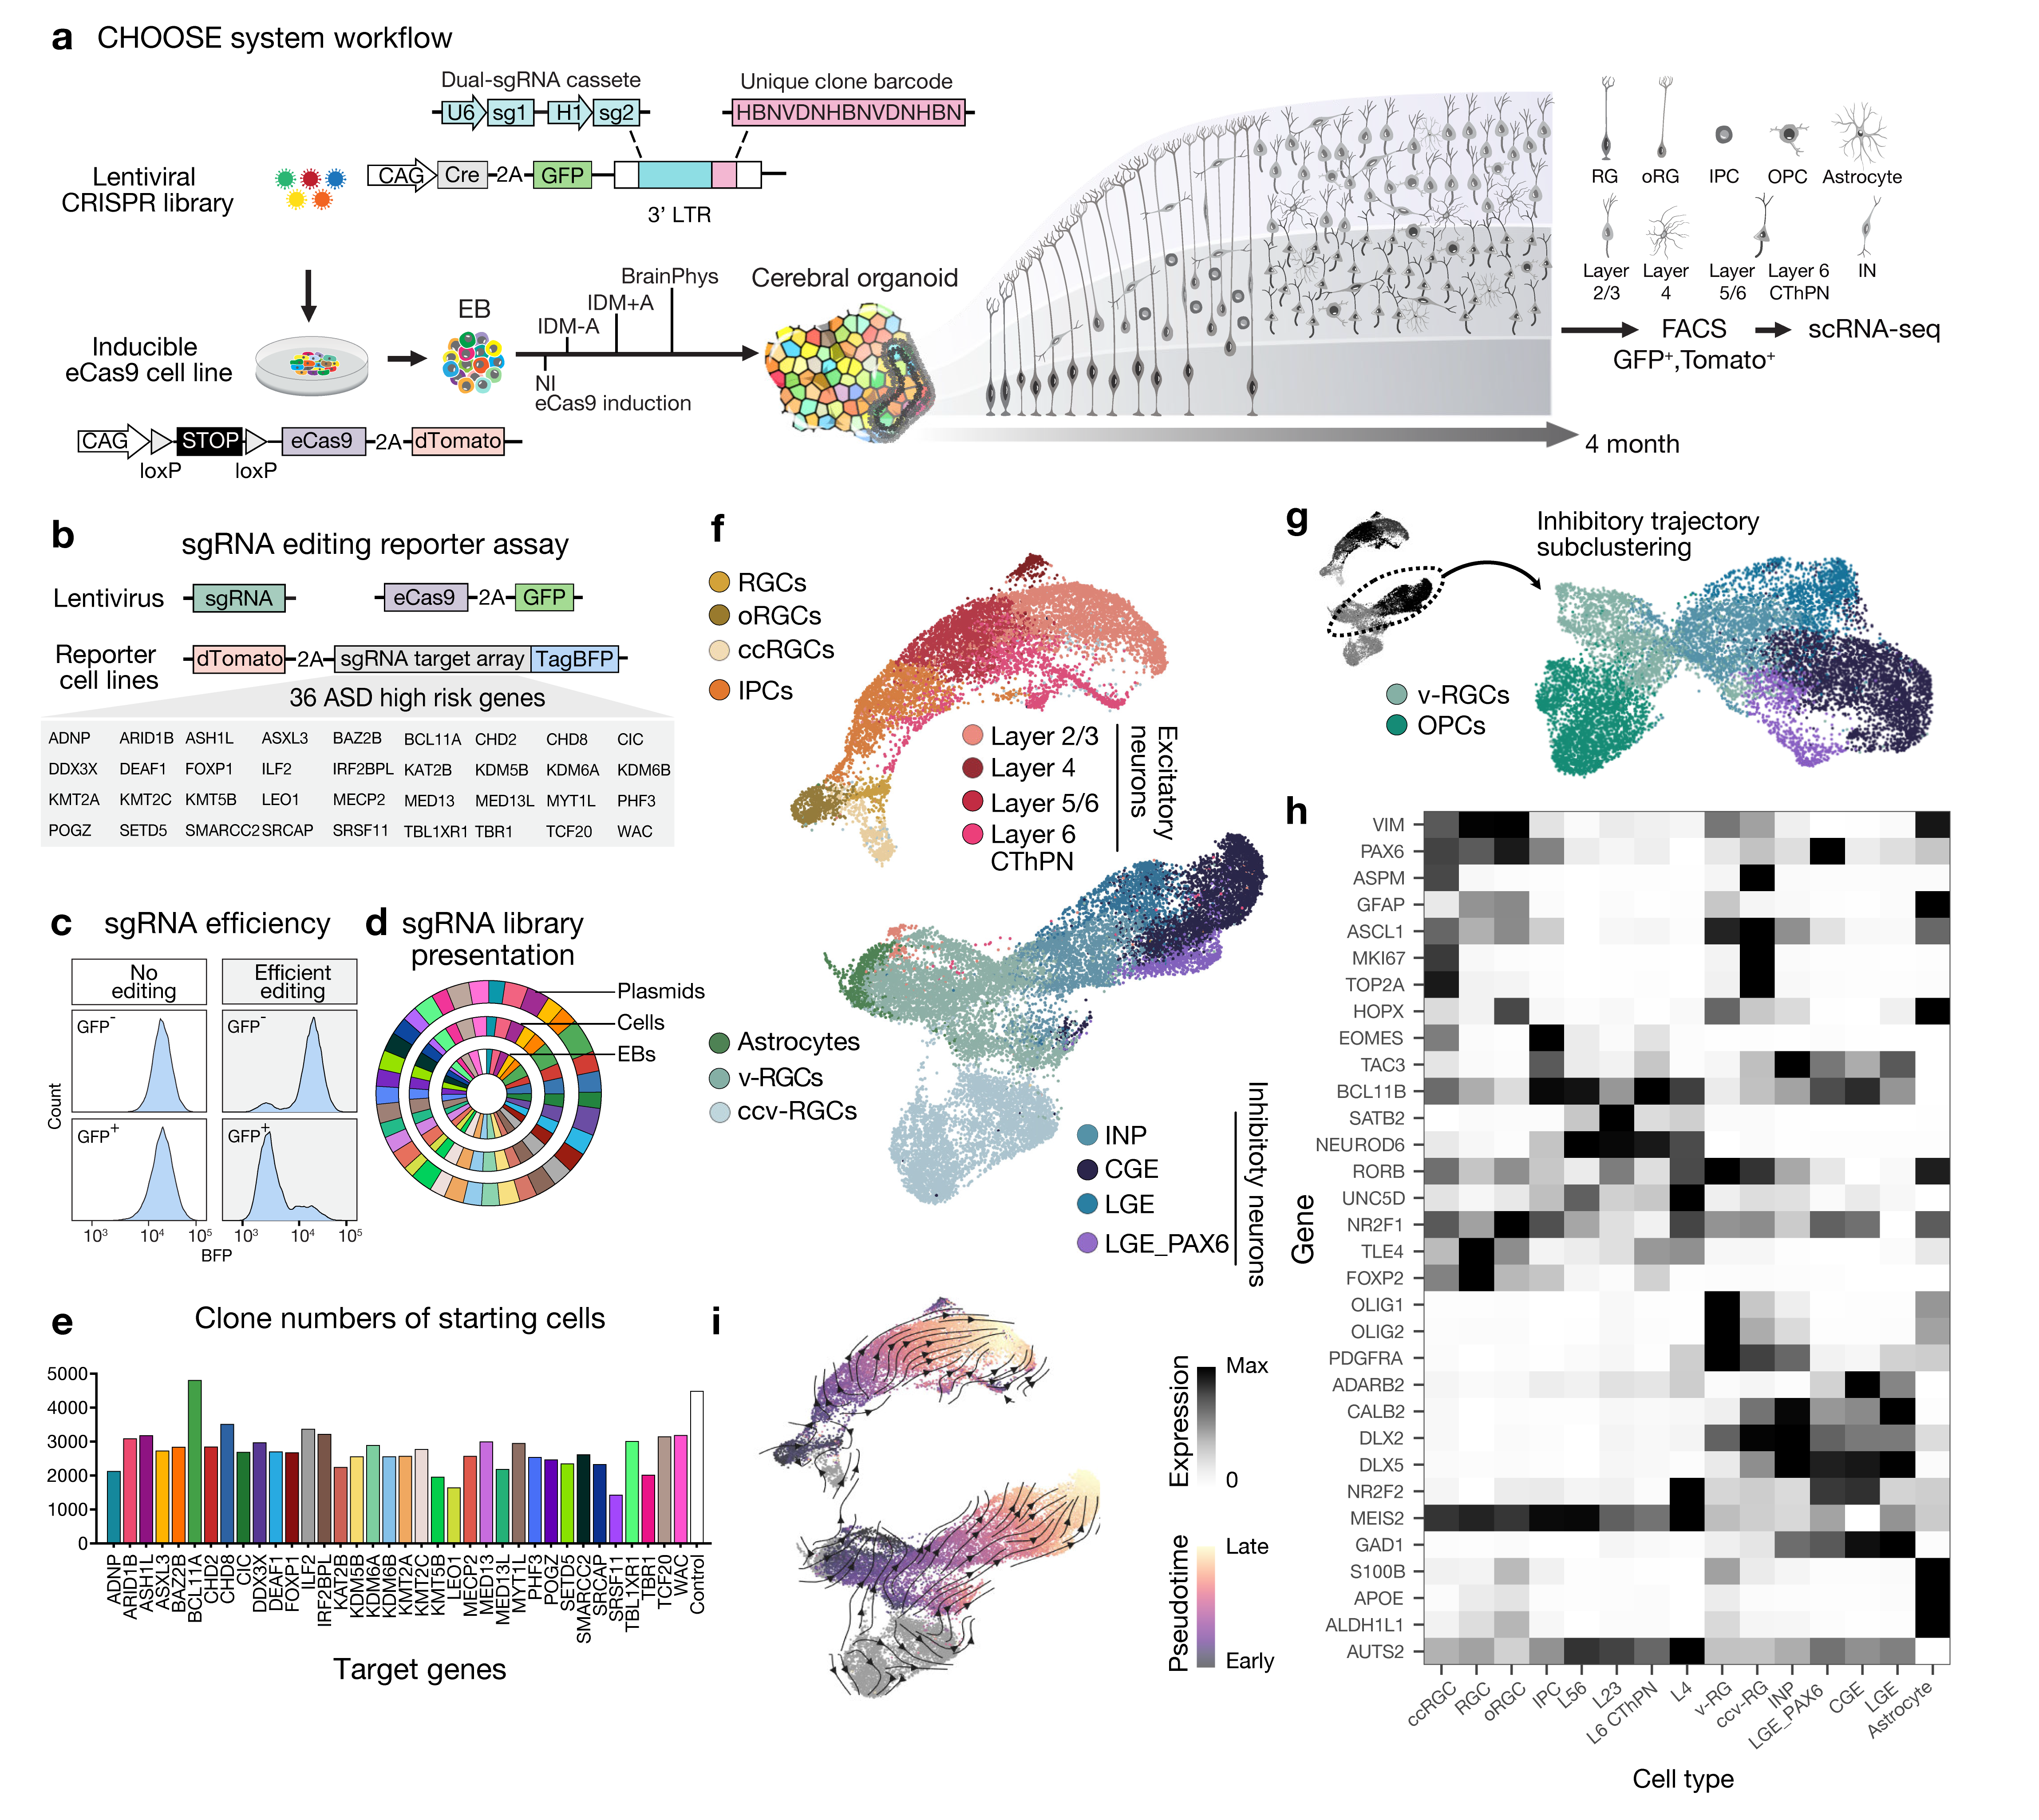
\includegraphics[width=\textwidth]{figures/asd/Figure_1}
    \caption{\textbf{The CHOOSE system for multiplexed screening of ASD risk genes in human cerebral organoids.}
    a, CHOOSE system overview. Barcoded dual-sgRNA cassette located within the 3' LTR of the lentivirus. b, Reporter assay to test gRNA efficiencies for 36 ASD risk genes. c, Editing efficiencies of gRNAs determined by flow-cytometry. Plots show examples of gRNAs with no or efficient editing. d, sgRNA sequence read distributions of gRNAs sequenced from the ASD plasmid library, lentivirus infected hESCs, and EBs at day 5. e, Numbers of clones from the starting hESCs for each perturbation used to generate mosaic cerebral organoids. f, UMAP embedding of the scRNA-seq dataset containing dorsal and ventral telencephalon trajectories. g, Subclustering and UMAP embedding of the ventral telencephalon trajectory excluding astrocytes and ccv-RGC to annotate OPC clusters. h, Heatmap shows the expression of marker genes in different cell types. i, RNA velocity and velocity pseudotime inference in dorsal and ventral trajectories to show developmental directions.}
    \label{fig:asd1}
\end{figure}

\topparagraph{Single-cell loss-of-function screening in clonally barcoded organoids}
Single-cell RNA sequencing (scRNA-seq) is a high-throughput method for analyzing cellular heterogeneity of complex tissues. To establish an organoid system that enables CRISPR perturbations with single-cell transcriptomic readout, we made use of a human embryonic stem cell (hESC) line that expresses an enhanced specificity SpCas9 (eCas9) with significantly reduced off-target effects and is controlled by an upstream loxp stop element13 (Figure 1a). To regulate the eCas9 induction, we engineered a lentiviral vector to deliver a 4-hydroxytamoxifen (4-OHT)-inducible CRE recombinase and a dual single-guide RNA (sgRNA) cassette (Figure 1a). In this cassette, two sgRNAs targeting the same gene are expressed under the U6 or H1 promoter. The dual-gRNA is located within the 3' long terminal repeat (LTR) of the lentiviral vector and is thus transcribed by RNA polymerase II to be captured by scRNA-seq assays14. To ensure efficient generation of loss-of-function alleles, we determined the editing efficiency of the candidate sgRNAs for each target gene using a flow cytometry-based gRNA reporter assay (Figure  1b, Figure S1a). In this assay, a pre-assembled array of gRNA-targeting sequences is fused with TagBFP and is transduced in 3T3 cells to generate reporter cell lines. sgRNA and eCas9 are then delivered to the reporter cell lines by lentiviruses. Successful genome editing causing frameshift mutations leads to the loss of BFP fluorescence, allowing us to quantitatively evaluate gRNA efficiency in a large cell population (Figure  1c, Figure S1b, c). Using our reporter assay, we selected efficient sgRNA pairs for 36 ASD genes (Figure S1d-e, Table 1).  
We cloned sgRNA pairs individually and pooled them equally to construct a lentiviral plasmid library. To ensure that the lentiviral integration frequency is limited to one per cell, we used a low infection rate of 2.5\%15 (Figure S2a-c). Importantly, the development of human brain tissues exhibits generation of cell clones with highly variable sizes both in vivo and in vitro13,16. To monitor the clonal complexity of the founder cells, we introduced a unique clone barcode (1.4 X 107 possible combinations) for each dual-sgRNA cassette to label individual lentiviral integration events (Figure  1a, Figure S3a-c). Our analysis showed that the homogeneous distribution of the gRNAs presented in the plasmid library and in hESCs at the time of infection and was also maintained after the formation of embryoid bodies (EBs) (Figure 1d). In addition, for each gene perturbation, we obtained an average of 2,770 unique clones, which we used to generate mosaic EBs (Figure 1e). Altogether, we established a highly efficient and controlled pooled screening system with high clonal complexity in the organoid. 

\topparagraph{CHOOSE cerebral organoids generate a high diversity of telencephalic cell types} 
Cortical abnormalities are a key pathological feature of ASD6,17. Many ASD risk genes related to transcriptional regulation and chromatin remodeling pathways are crucial for cortical development18,19. However, it was previously not possible to explore which cell types are affected when and how by these risk genes. We thus sought to leverage our methodology to explore loss-of-function phenotypes for 36 transcriptional control genes with high causal confidence (SFARI database category 1 genes)5.
We used previously established protocols which reproducibly generate human telencephalon tissues from human pluripotent stem cells20,21 (Figure S4a-c). Single-cell transcriptomic profiling (10X Genomics Chromium) of cerebral organoids at 4 months revealed a large diversity of cell types composing the developing dorsal and ventral telencephalon (Figure 1f-h, Figure S5a-c; 31 cerebral organoids). We identified progenitor cells with dorsal (PAX6) or ventral (ASCL1, OLIG2) origins. In the dorsal telencephalon trajectory, we identified radial glial cells (RGCs), cycling RGs (ccRGCs; ASPM), outer radial glial cells (oRGCs; HOPX) and intermediate progenitor cells (IPCs; EOMES). Dorsal progenitors differentiated into excitatory neurons of specific layer identities, including layer 5/6 neurons (L5/6; BCL11B), layer 6 cortical thalamic projection neurons (L6 CThPN; FOXP2, TLE4)22,  layer 4 neurons (L4; RORB, UNC5D, NR2F1)23,24 and layer 2/3 neurons (L2/3; SATB2). Progenitors from the ventral telencephalon differentiated into interneuron precursor cells (INPs; DLX2), which generated interneurons with lateral ganglionic eminence (LGE) origin (LGE-IN; MEIS2), or caudal ganglionic eminence (CGE) origin (CGE-IN; NR2F2)25. Interestingly, we found a cluster of interneurons expressing MEIS2 and strong PAX6 (LGE\_PAX6), which transcriptionally resembles mouse olfactory bulb precursors, and was recently reported to be redirected to white matter specifically in primates26. In addition to neuronal populations, we also identified glial cell populations including astrocytes (S100B, APOE, ALDH1L1) and oligodendrocyte precursor cells (OPC; OLIG2, PDGFRA) (Figure 1f-g). RNA velocity analysis27 {Bergen NatBiotech 2020} revealed general developmental trajectories from neural progenitor cells to neuronal populations in both the dorsal and ventral telencephalon (Figure 1i). Taken together, our scRNA-seq dataset of 4-month-old cerebral organoids recapitulates diverse telencephalic cell types that are present in the developing human brain. 

\topparagraph{Perturbing ASD risk genes depletes dorsal IPCs and enriches ventral RGCs}
The presence of the large cellular diversity detected in our organoids allows us to systematically assess, compare, and categorize the effects of perturbations on cell fates. Using targeted amplification and hemi-nested emulsion PCR, we first recovered sgRNA information and assigned 28,344 cells to unique sgRNAs (Methods, Figure S5d-e). With a Cochran-Mantel-Haenszel test stratified by library, we then measured the differential abundance of overall cell populations from dorsal (D) versus ventral (V) telencephalon (hereafter referred to as dorsal and ventral lineage, respectively), as well as of each individual cell type in perturbations versus control (non-targeting sgRNAs) (Figure 2a, Figure S6). 
We first detected significant changes in the ratio of dorsal to ventral (D-V) lineage (orange to purple, Figure 2a, left) for 24 perturbations. Interestingly, in most perturbations (21/24) a lowered D-V ratio was detected. On the level of cell types, we detected abundance changes for 21 perturbations (red to blue, Figure 2a, right) with at least one cell type affected (CMH-test, FDR < 0.05). For example, perturbation of KMT2C led to an overall depletion of the dorsal lineage and enrichment of the ventral lineage, whereas 8 perturbations specifically targeted one cell type without affecting the others, such as ADNP (L2/3 enrichment), MED13L (L2/3 depletion), ILF2 (CGE\_IN enrichment), and DDX3X (CGE\_IN depletion). Perturbations of LEO1 and TCF20 caused an enrichment of L4 neurons, which is a cell population critical for rapid sensory response that serves as the first level of sensory signal processing in cortical neurons28. This is consistent with the fact that sensory and in particular auditory and visual processing concerns are one of the prevalent ASD symptoms29. 
Within the dorsal lineage, we identified depletion of IPCs as a strong convergent effect (Figure 2a, ARID1B, BCL11A, CHD2, KAT2B, KMT2C, MECP2, MED13, PHF3, SETD5, TBL1XR1), whereas within the ventral lineage, progenitor cells (v-RGCs and ccv-RGCs) and INPs were among the most affected cell populations with an enrichment in most perturbations (e.g. CIC, CHD2, MED13, PHF3 and TBL1XR1). Interestingly, perturbations of three BAF complex members ARID1B, BCL11A and SMARRC2, all lead to an enrichment of v-RGCs, suggesting a critical role of the BAF complex in regulating the cell fate specification of ventral lineages. With respect to ventral telencephalic neurons, we detected LGE-IN enrichment in 7 perturbations, while 3 perturbations caused CGE-IN changes with either a depletion or enrichment effect, indicating an interneuron subtype-specific response to ASD genetic perturbations during development. Beyond neuronal lineages, we found that astrocytes were affected by 2 perturbations with opposite outcomes (enrichment in DEAF1 and depletion in LEO1 perturbations). 
Collectively, the CHOOSE system allowed us to simultaneously investigate the effects of numerous ASD genes on cell fate determination. We found that progenitor populations, including dorsal IPCs and ventral RGCs, are among the most affected cell types, which indicates that ASD pathology could already emerge as early as the neural progenitor stage.  

\begin{figure}[t!]
    \centering
	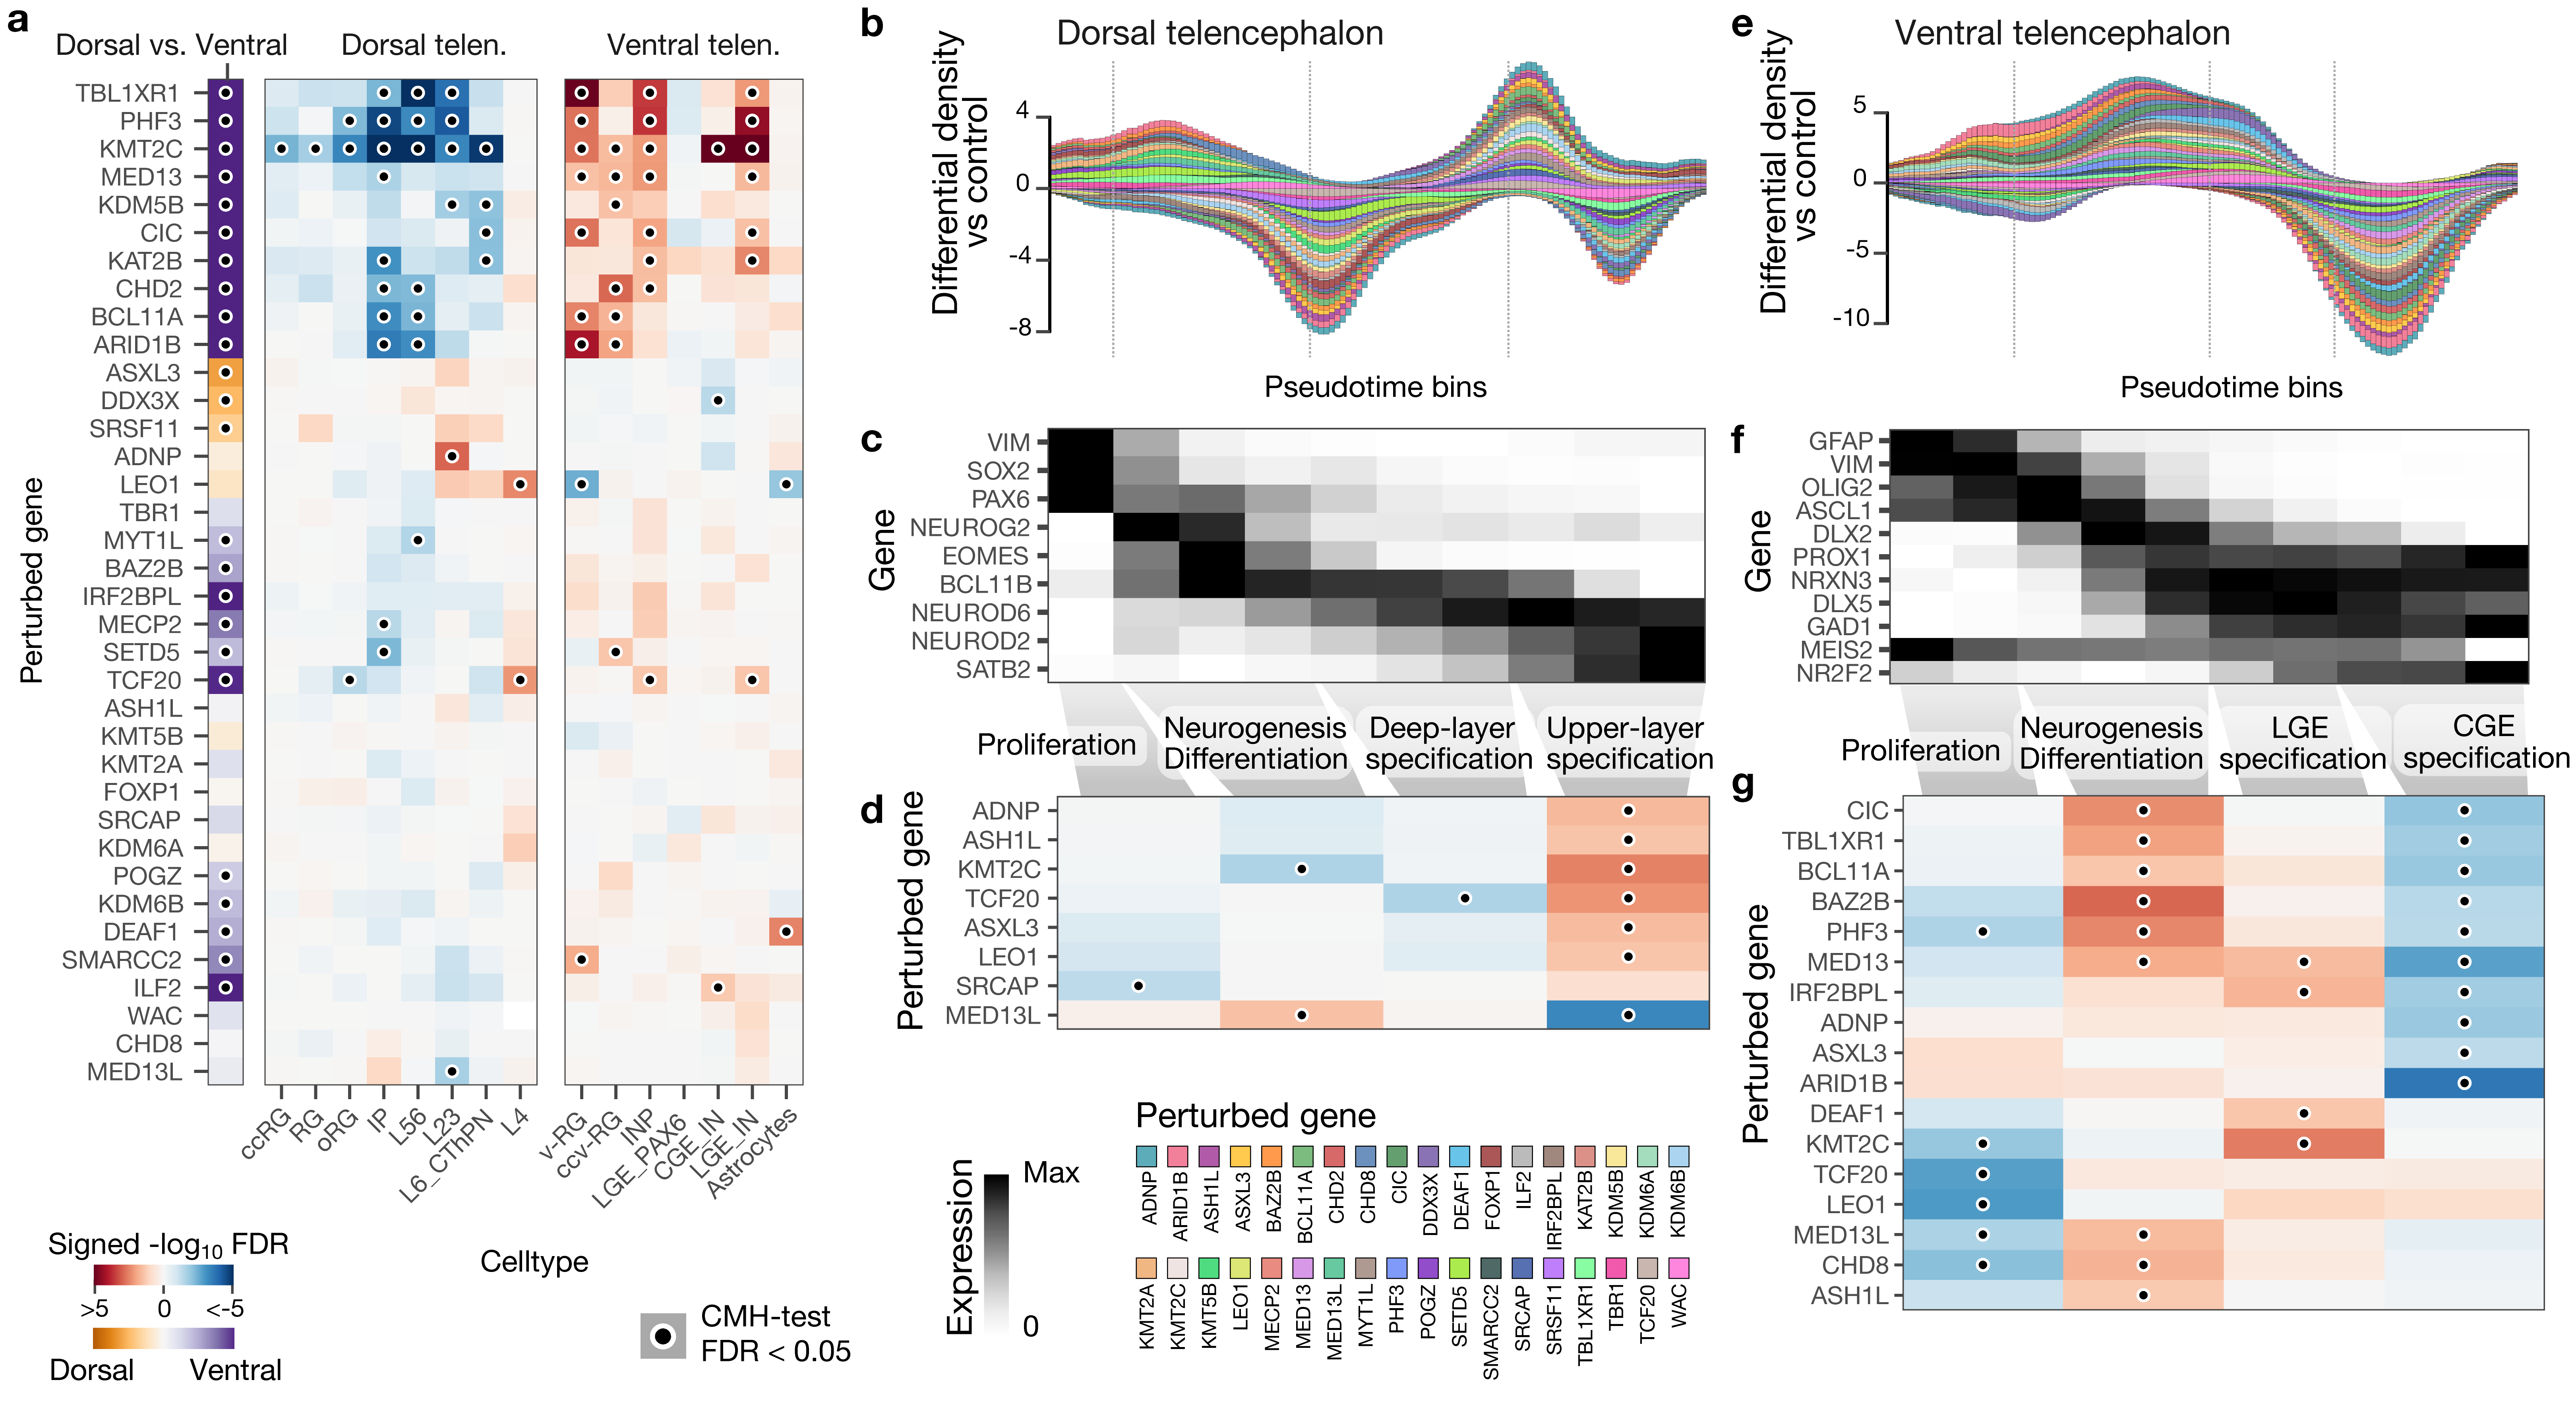
\includegraphics[width=\textwidth]{figures/asd/Figure_2}
    \caption{\textbf{Cell type and developmental process-specific effects of perturbations of ASD risk genes.}
    a, Heatmap shows enrichment of gRNAs versus control in the dorsal versus ventral lineage (left, purple to orange) and individual cell types (middle and right, blue to red). Colors indicate the sign of the log odds ratio multiplied by the -log10 FDR-corrected p-value of a CMH test stratified by library (signed -log10 FDR). b, e, Accumulative differential density of perturbations versus control across a binned pseudo-temporal axis. Each color represents one perturbation. c, f, Heatmaps show the expression of genes used to define developmental stages. d, g, Heatmaps show enrichment of gRNAs in annotated developmental stages for each trajectory.}
    \label{fig:asd2}
\end{figure}

\topparagraph{Perturbing ASD risk genes impairs upper-layer neuronal specification and ventral progenitor differentiation} 
scRNA-seq captures transcriptional dynamics in developing tissues and therefore allows the analysis of cell state transitions {Trapnell NatBiotech 2014} 27 . Using RNA velocity and gene expression patterns, we first defined developmental stages along both the dorsal and ventral telencephalic trajectory covering progenitor proliferation (VIM), onset of neurogenesis (dorsal: NEUROG2; ventral: ASCL1), differentiation (dorsal: BCL11B, NEUROD6; ventral: ASCL1, DLX2, OLIG2), and neuronal subtype specification (dorsal: NEUROD2, NEUROD6, BCL11B, SATB2; ventral: MEIS2, NR2F2, DLX5) (Figure 2c-f). We then calculated the differential density for cells of each perturbation versus control along a binned pseudo-temporal axis within the dorsal and ventral telencephalic trajectory, respectively (Figure 2b-e, Figure S7). 
The developmental stage-based differential testing provides additional resolution on the effects of perturbations on cell states. For example, in the dorsal trajectory, we found an accumulative high density of perturbed cells in an early stage of upper layer specification, as indicated by decreasing BCL11B and increasing SATB2 expression (Figure 2b-c). Differential abundance tests revealed that perturbations of ASH1L, ASXL3, and TCF20 were enriched in the upper layer specification stage (Figure 2d) despite the fact that we did not detect differential abundance of upper layer neurons when comparing to all cell types (Figure 2a). Thus, the combined analyses of cell states and developmental progression favor the hypothesis that perturbations of these genes cause accelerated upper layer neurogenesis. Additionally, analyses of the ventral trajectory show an enriched density at the stages of neurogenesis and differentiation caused by multiple perturbations (high DLX2 and OLIG2 expression), suggesting that this developmental process is susceptible to ASD genetic perturbations (Figure 2e-g). Interestingly, other perturbations which did not cause cell type compositional changes nonetheless affected specific processes along a developmental trajectory. For example, disrupting the chromatin remodeler SRCAP results in reduced dorsal neural stem cell proliferation, which is consistent with a recently identified role of SRCAP in stem cell self-renewal30(Figure 2d). 
Overall, our perturbation-specific characterizations of differential abundance of cell types as well as of stages along developmental trajectories together create a unique resource to delineate ASD high-risk gene loss-of-function phenotypes.

\begin{figure}[b!]
    \centering
	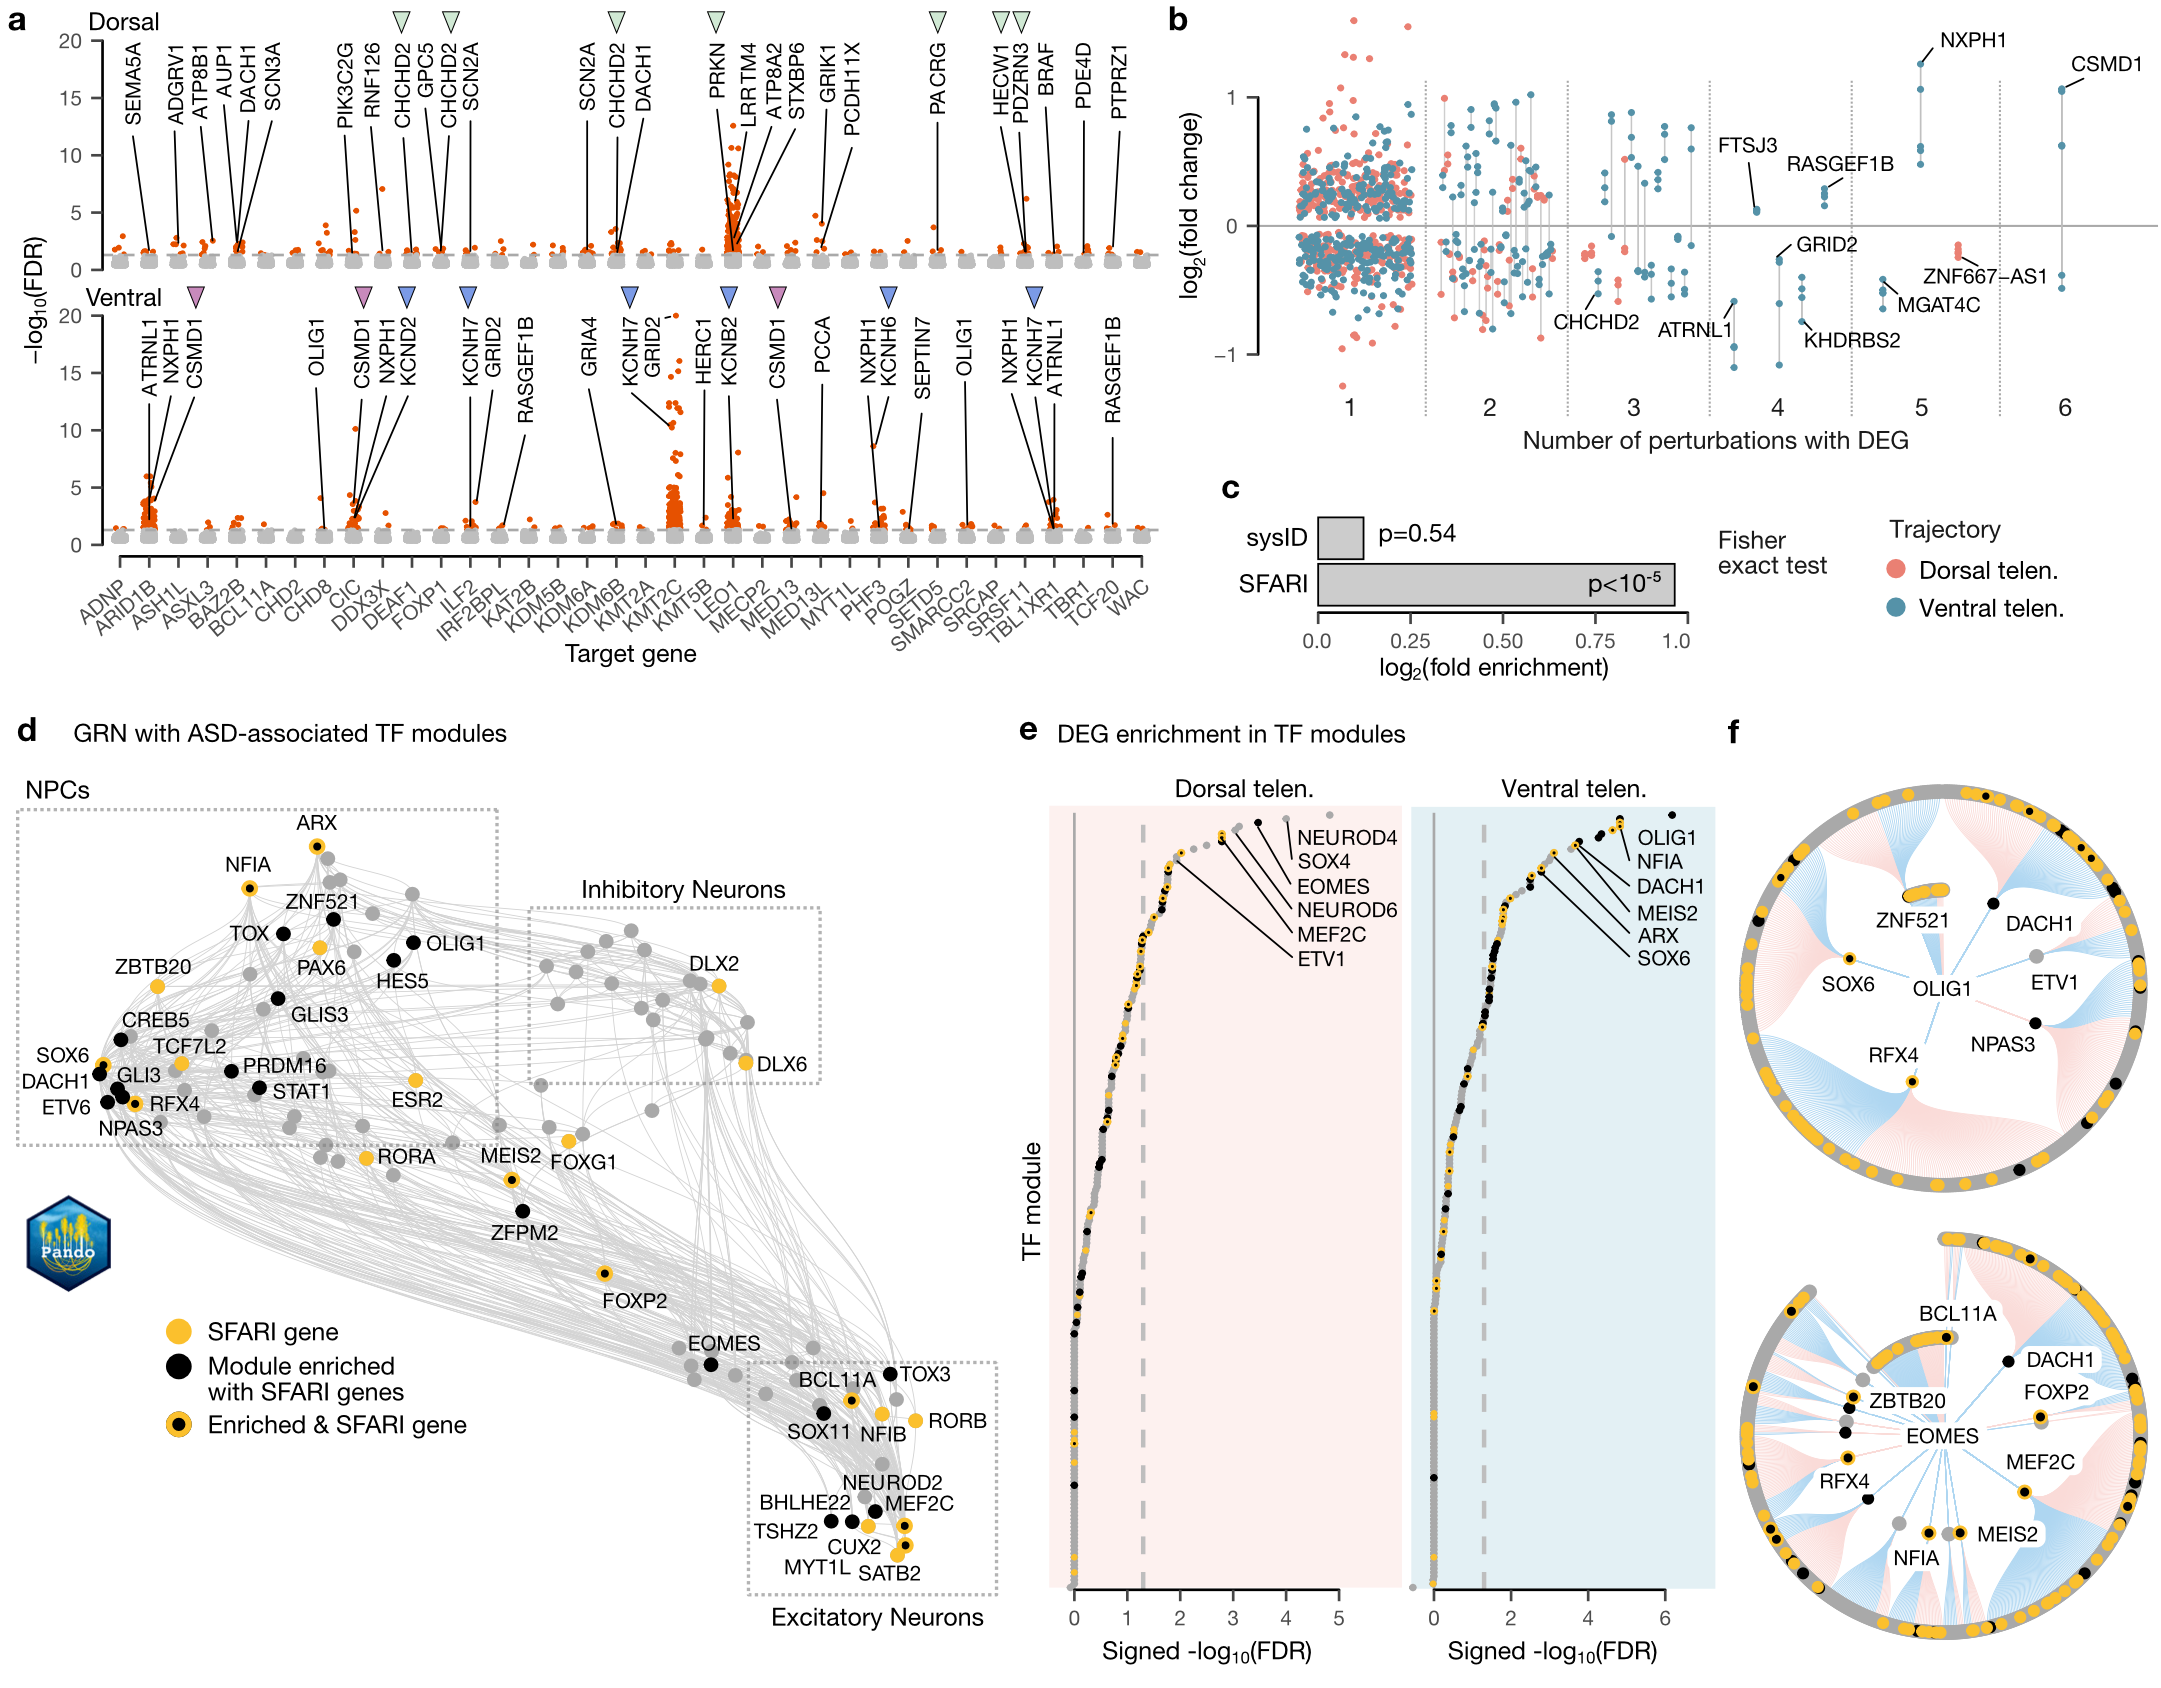
\includegraphics[width=\textwidth]{figures/asd/Figure_3}
    \caption{\textbf{Dysregulated gene expression and regulatory networks caused by perturbations of ASD risk genes.}
    a, Manhattan plots show DEGs detected in dorsal (top) and ventral (bottom) trajectories from each genetic perturbation. Green arrowheads indicate genes associated with PD (CHCHD2, PRKN, PACRG) or the ubiquitin system (PRKN, HECW, PDZRN3). Blue arrowheads indicate genes encoding VGKCs. b, Jitter plot shows frequency of DEGs detected from all perturbations separated by dorsal (blue) and ventral (orange) trajectories. Points belonging to the same gene are connected with a gray line. c. Enrichment test of TOP-DEGs (top 30 DEGs from each perturbation) in ID (sysID database) or ASD (SFARI database) genes. The p-value was obtained from a Fisher exact test. d, GRN of 4-month-old cerebral organoids inferred by Pando showing developmental TF modules constructed based on their co-expression and interaction strengths. ASD-specific TF modules are highlighted in yellow (SFARI genes) and/or black (regulator of SFARI genes). e, Lolliplots show CHOOSE-DEG enriched TF modules in dorsal and ventral trajectories. f, Circular GRN plots show primary and secondary targets of OLIG1 and EOMES. ASD-specific TF modules are highlighted in black/yellow as described above.}
    \label{fig:asd3}
\end{figure}

\topparagraph{CHOOSE identifies lineage-specific dysregulated genes}
To further assess molecular changes caused by each perturbation, we performed differential gene expression analysis comparing each perturbation to control within dorsal and ventral lineages and detected 885 differentially expressed genes (DEGs) in total (Figure 3a, top, dorsal lineage; bottom, ventral lineage; Supplementary Data 1). We ranked DEGs by detection frequency and discovered that certain genes, or gene families, are identified in multiple perturbations (Figure 3b). Interestingly, in the dorsal lineage, perturbations of DEAF1, FOXP1 and KDM6B, all lead to the down-regulation of CHCHD2 (Figure 3a), a gene encoding a mitochondrial coiled-coil-helix-coiled-coil-helix domain containing protein and associated with Parkinson's disease (PD)31. CHCHD2 was also found to be downregulated in both excitatory and inhibitory neuronal lineages in postmortem brain tissues from several autism patients32. Additionally, 4 other PD or ubiquitin proteasome pathway associated genes are dysregulated, including PRKN (LEO1 perturbation), PACRG (SETD5 perturbation), HECW1 and PDZRN3 (SRSF11 perturbation) (Figure 3a). Of note, ubiquitin genes have been identified to cause autism33. Our findings support the role of a dysregulated ubiquitin proteasome system in the pathophysiology of ASD during development. In the ventral lineage, the most frequently detected DEG is the adhesion molecule CSMD1 (Figure 3a, b), which is upregulated by ARID1B, CIC, MED13, and PHF3 perturbations, and downregulated by LEO1 and KMT2C perturbations.
Ion channel deficiency has been implicated in NDDs and is strongly associated with neurological conditions such as epilepsy34. We found that genes encoding voltage-gated potassium channels (VGKCs), including KCNB2, KCND2, KCNE5, KCNH6, and KCNH7, are differentially expressed in at least one of seven perturbations (ARID1B, CIC, ILF2, KMT2C, LEO1, PHF3, TBL1XR1) in the ventral lineage (Figure 3a). VGKCs play an important role in regulating neuronal excitability and have been linked to ASD35. Interestingly, genes related to sodium channels are specifically dysregulated in the dorsal lineage (Figure 3a, top, SCN2A upregulation in ILF2 and KDM6A perturbations, SCN3A upregulation in BAZ2B perturbation), but not in the ventral lineage. These data suggest a lineage-specific channel dysregulation caused by ASD genetic perturbations. 


\topparagraph{CHOOSE combined with GRN inference from single-cell multiome data identifies ASD-specific transcription regulatory modules}
When combining the DEGs from all perturbations, we found that they were significantly enriched in risk genes associated with ASD (SFARI database, 1031 genes; ~2-fold enrichment, p < 10-5; Figure 3c, d; Supplementary Data 1). Interestingly, however, we did not observe enrichment in risk genes for other neurodevelopmental disorders such as intellectual disability (ID; SysID database, 936 primary ID genes; Figure 3c) indicating that certain biological processes and developmental regulatory programs are specifically susceptible to ASD-associated gene perturbations. To explore these potential gene regulatory 'hubs', we first generated single-cell multiomic data including single cell transcriptome and chromatin accessibility modalities from 4-month-old cerebral organoids (Figure S8a-d). Using Pando36, we could harness these multimodal measurements to infer a gene regulatory network of the developing telencephalon and extract sets of genes regulated by each transcription factor (TF modules) (Figure S8e,f). We visualized this TF network using a UMAP embedding {McInnes 2018 https://arxiv.org/abs/1802.03426; Becht 2019 NatBiotech}, which revealed distinct groups of TFs active in NPCs (PAX6, GLI3, OLIG1), inhibitory neurons (DLX2, DLX6) and excitatory neurons (NEUROD2, NFIB, SATB2) as well as regulatory interactions between the TFs (Figure 3e). 
To test whether regulatory sub-networks indeed exist at which ASD risk genes accumulate, we tested all TF modules for enrichment with SFARI genes. We found significant enrichment for a set of 40 TFs (adjusted Fisher test p-value < 0.01, >2-fold enrichment) (Figure S8g), among which 14 TFs are ASD risk genes (e.g. NFIA, BCL11A, MEF2C), and others are regulators of ASD risk genes (e.g. OLIG1, DACH1, EOMES) (Figure 3e). All TF regulatory modules enriched in SFARI genes together form an ASD-specific sub-GRN.
Next, we assessed the transcriptomic effect of ASD genetic perturbations in the context of the inferred GRN. We performed enrichment tests on perturbation-induced DEGs (CHOOSE-DEGs) from dorsal and ventral telencephalic cells separately. We found that, similar to ASD risk genes, CHOOSE-DEGs were enriched in specific TF modules (Figure 3f). In the ventral telencephalic cells, OLIG1 and NFIA were most strongly affected, whereas dorsal telencephalon-specific DEGs were most strongly enriched in NEUROD4, SOX4 and EOMES modules. Interestingly, some of the ASD-specific TF modules were among the most strongly enriched in CHOOSE-DEGs, supporting their role in ASD-specific gene dysregulation (Figure 3f). We finally present gene regulatory subnetworks of OLIG1 and EOMES, two important genes whose regulomes are both enriched in ASD risk genes and strongly affected by ASD genetic perturbations (Figure 3g). 
Taken together, we have characterized gene expression changes for each genetic perturbation in both dorsal and ventral telencephalon and uncovered novel molecular programs shared between different perturbations. Leveraging GRN inference from single-cell multiomic data, we further identified ASD-specific TF modules during cortical development and critical regulatory hubs underlying the detected gene expression changes.

\begin{figure}[b!]
    \centering
	\includegraphics[width=\textwidth]{figures/asd/Figure_4}
    \caption{\textbf{Perturbation of ARID1B increases the transition of v-RGCs to early OPCs.}
    a, Circular projection of terminal fate probabilities shows ventral telencephalon differentiation trajectories. b, Trajectory branches defined by gene expressions of DLX2 (INP), DLX5 (IN), OLIG2 (early OPC) and PDGFRA (late OPC). c, Differential density of cells with ARID1B perturbation versus control. d, Bar graph shows cells within the v-RGCs are positive for DLX2 (68.6\% versus 81.5\%), OLIG2 (19.6\% versus 36.2\%) and both (9.8\% versus 30.6\%) in control versus ARID1B perturbation. e, Box plots showing transition probabilities of control and ARID1B perturbed ventral progenitor cells towards OPCs. Middle line depicts the median; box marks the 25\% and 75\% quantiles. f, Immunohistochemistry for early OPCs (OLIG2) and INPs (DLX2) of day 40 ventralized brain organoids derived from control (c. 220dupG repair) and two ARID1B patient iPSCs. Scale bar, 200 $\mu$m. g, Violin plots (all data points and median values) show numbers of cells positive for OLIG2 and/or DLX2. Control, n =108 areas from 13 organoids, 4 batches; ARID1B+/- (c.2201dupG), n = 104 areas from 15 organoids, 4 batches; ARID1B+/- (6q25.3del), n = 94 areas from 15 organoids, 3 batches. One-way ANOVA post hoc Tukey test. ***P<0.01. h, Prenatal magnetic resonance imaging scan and 3D reconstruction of LGE and CGE (marked as GE) from age matched controls and ARID1B patient showing enlarged GE in the patient. Quantified in Figure S10c. Scale bar, 1 cm. I, Diagram showing ARID1B perturbation-induced cellular responses of ventral progenitors.}
    \label{fig:asd4}
\end{figure}

\topparagraph{ARID1B perturbation increases the transition probability of v-RGCs to early OPCs}
Amongst the 36 genes, we found that ARID1B perturbation causes one of the most dramatic enrichments of v-RGCs (Figure 2a). Interestingly, the OLIG1 regulatory module was also specifically enriched in DEGs caused by ARID1B perturbation (Figure S9). These data intrigued us to further investigate how v-RGCs are affected by ARID1B perturbation. We used Cellrank37 to resolve the developmental trajectories leading to different inhibitory neuron types as well as OPC populations (Figure 4a). We visualized the terminal fate probabilities for each cell as a circular projection {Velten 2017 NatCellBio}, which revealed a distinct differentiation trajectory from ventral progenitors towards early OPCs (OLIG2, PDGFRA) and a branching of INPs (DLX2) into different inhibitory neuronal fates (DLX5) (Figure 4b). We found that ARID1B perturbed cells were strongly enriched in the OPC trajectory and had a higher percentage of OLIG2+ v-RGCs (Figure 4c-d). This is an interesting finding given that OLIG2 is known to regulate progenitor self-renewal at earlier developmental stages and is a master regulator for oligodendrocyte lineage specification in the ventral telencephalon38,39. We then analyzed fate transition probabilities of ventral progenitors and found that ARID1B-perturbed v-RGCs have significantly higher transition probabilities towards early OPC than neuronal fates (Figure 4e).
Loss-of-function mutations in ARID1B have been identified to cause ID and ASD5,40. To confirm whether our findings are relevant to human disorders, we recruited two patients with ARID1B heterozygous mutations. Patient 1 harbors a nucleotide duplication (c.2201dupG) that results in a frameshift and an early STOP codon, and Patient 2 carries a microdeletion (6q25.3del) that includes exon 8 and the downstream region of the ARID1B locus (Figure S10a, b). We established iPSC lines from both patients and a mutation-corrected cell line for patient 1 as an isogenic control. We then generated cerebral organoids with enriched ventral telencephalon regions by adding patterning factors SAG and IWP2 and investigated the behavior of v-RGCs at day 4041. In organoids from both patients, we observed considerably increased OLIG2+ cells, as well as DLX2+, and DLX2+/OLIG2+ cells compared to the control, which is in line with our previous findings (Figure 4g). Finally, to further explore the potential consequences of such defects in patients, we analyzed the prenatal brain structure of patient 2 using intra-uterine super-resolution MRI obtained at two gestation stages (GW22 and GW31). 3D reconstruction of the LGE and CGE, sources of ventral telencephalon progenitors, revealed an enlarged volume compared to multiple age-matched controls at both stages (Figure 4h, Figure S10c). Taken together, the enrichment of v-RGCs and ccv-RGCs (Figure 2a), the higher transition probability of v-RGCs to early OPCs, and the increased proportion of OLIG2+ cells in our CHOOSE experiment and in organoids generated from two patient iPSC lines, all suggest that ARID1B perturbation leads to abnormal ventral progenitor expansion and aberrant cell fate specification (Figure 4i). We propose that this translates to the enlarged volume of the LGE and CGE in the ARID1B patient.


\subsection{Discussion}
We have developed the CHOOSE system to characterize the loss-of-function phenotypes of 36 high-risk ASD genes across dozens of cell types spanning early brain developmental stages in human cerebral organoids. Our findings provide a developmental and cell-type specific phenotypic database for ASD high-risk gene loss-of-function research, which will shed light on the disease pathogenesis.
We assessed phenotypes affecting dorsal and ventral telencephalic lineages during brain development. IPCs are transit-amplifying dorsal progenitors which generate neurons for all cortical layers and contribute to the evolutionary expansion of the human cortex42,43. We found that IPCs appeared to be particularly susceptible to ASD genetic perturbations. Interestingly, some of the perturbed genes have previously been suggested to play a role in IPC regulation within a disease context. For example, brain organoids derived from a patient with an MECP2 mutation were shown to have decreased number of IPCs44. 
In the ventral lineage, we identify a strong enrichment of progenitor cells, including v-RGs and ccv-RGs, which are the major progenitor pools differentiating into interneurons and oligodendrocytes38,45. Compared to CGE-INs, which can be depleted or enriched, we found that LGE-INs appeared to be only enriched by perturbations. Our results establish a basis for dissecting the relevance of CGE and LGE-IN dysfunction in ASD pathophysiology, which is important considering recently discovered human-specific CGE and LGE interneuron migration features and function21,26,46.
Additionally, DEG analyses revealed that multiple perturbations impaired the same molecular processes, which may be critical for the development of ASD pathophysiology. For example, we found that specifically in the dorsal lineage, genes related to Parkinson's disease and the ubiquitin system are frequently dysregulated. Interestingly, parkinsonism features have been reported in older autistic adults47. Our findings further suggest that ubiquitin dysfunction could already be emerging during early development stages. Furthermore, we constructed a GRN underlying telencephalon developmental trajectories and identified ASD-specific regulatory modules in dorsal and ventral lineages. The OLIG1 regulatory module is particularly interesting as many of its downstream targets are ASD risk genes (SFARI database). This regulatory module was previously identified as being important for oligodendrocyte differentiation in the developing human cerebral cortex19. Thus, our findings highlight the involvement of the oligodendrocyte lineage in the development of ASD pathophysiology.
Finally, we discovered that loss of ARID1B, a BAF complex component, leads to an increased transition of ventral progenitors to early OPCs.  Interestingly, the OLIG1 regulatory module is also affected by ARID1B perturbation. The role of the BAF complex in oligodendrocyte generation and maturation has been mainly established by studying one of its components, SMARCA4, which is required for OPC differentiation48. Considering the temporal and cell-type specific expression of each BAF subunit, it would be interesting to investigate how ARID1B or other subunit-mediated chromatin remodelers regulate oligodendrocyte specification and how their dysfunction contributes to neurodevelopmental disorders.
The ability to determine cell-type specific contributions to genetic disorders in a systematic, scalable, and efficient manner will greatly facilitate our understanding of disease mechanisms. As the CHOOSE system provides a robust, precisely controlled screening strategy, we anticipate it will be widely applied beyond brain organoids to study disease-associated genes. 


\subsection{Methods}

\paragraph{Data availability}
Raw sequencing data will be deposited on ArrayExpress. Processed Seurat objects will be deposited on Zenodo and will be made available under restricted access before publication. The Pando R package is available on GitHub: \\
(https://github.com/quadbiolab/Pando) \\
Other custom code used in the analyses is deposited on GitHub: \\ 
(https://github.com/quadbiolab/ASD\_CHOOSE).

\paragraph{Acknowledgements}
We are grateful to the patients and their families for participating in this study. We thank all Knoblich lab members for support and discussions; François Bonnay, Emmanouella Chatzidaki, Oliver L. Eichmüller, Ramsey Najm, and Jaydeep Sidhaye for comments on the manuscript; Mario Nezhyba and Thomas Lendl from the IMP/IMBA Biooptics Facility for technical support; Alexander Vogt and Florentina Drochter from the VBCF NGS facility for scRNA-seq library preparation; the IMBA Stem Cell Core facility for generation of iPSC lines. Work in J.A.K.'s laboratory is supported by a SFARI pilot award (724430), the Austrian Federal Ministry of Education, Science and Research, the Austrian Academy of Sciences, the City of Vienna, and the SFB F78 Stem Cell (F 7803-B). Work in B.T.'s laboratory is supported by the European Research Council (Organomics, B.T.; Braintime, B.T.), the Chan Zuckerberg Initiative DAF, an advised fund of the Silicon Valley Community Foundation (CZF2019-002440), the Swiss National Science Foundation (310030\_192604) and the National Center of Competence in Research Molecular Systems Engineering. A.V. is supported by an EMBO Fellowship (ALTF-1112-2019). J.S.F was supported by a Boehringer Ingelheim Fonds PhD fellowship.

\paragraph{Author contributions}
C.L. and J.A.K. conceived the project and experimental design and secured the funding. C.L., J.S.F., and J.A.K. prepared the manuscript with input from B.T. and all authors. C.L. performed all the experiments and analyzed the data with the help from T.R.B., A.V., A.M.P., and C.E., J.S.F. performed the analysis of scRNA-seq and multiome data under the supervision of B.T., M.S. and G.K. performed patient diagnosis and analyzed MRIs, C.M. generated iPSC lines under the supervision of N.S.C., U.E. provided sgRNA predication.   
 
\paragraph{Corresponding authors}
Correspondence and requests for materials should be addressed to C.L., B.T., or J.A.K.

\paragraph{Competing interests}
J.A.K. is on the supervisory and scientific advisory board of a:head bio AG (https://aheadbio.com) and is an inventor on several patents relating to cerebral organoids. The authors declare that they have no conflicts of interest.	


\paragraph{Stem cell and cerebral organoid culture conditions}
Feeder-free human embryonic stem cells (ESCs) or induced pluripotent stem cells (iPSCs) were cultured on hESC-qualified Matrigel (Corning, cat. no. 354277)-coated plates with Essential8 (E8) stem cell medium supplemented with BSA. H9 ESCs were obtained from WiCell. Cells were maintained in a 5\% CO2 incubator at 37 °C. All cell lines were authenticated using a short tandem repeat (STR) assay, tested for genomic integrity using SNP array genotyping, and routinely tested negative for mycoplasma.
Cerebral organoids were generated using a previously published protocol with modifications1. Briefly, cells were cultured to 70-80\% confluent and 16,000 live cells in 150 $\mu$l E8 medium supplemented with Revitacell (ThermoFisher, cat. no. A2644501) were added to each well of a U-bottom ultralow attachment 96 well plate (Corning, cat. no. CLS3473) to form EB. For eCas9 induction, 4-Hydroxytamoxifen (4-OHT, Sigma-Aldrich, cat. no. H7904) was added on day 5 at a concentration of 0.3 $\mu$g/ml. Neural induction was started on day 6. EBs were embedded in Matrigel (Corning, cat. no. 3524234) at day 11-12 based on morphology check. CHIR99021 (Merck, cat. no. 361571) at 3 $\mu$M was added from day 13 to 16 and medium was switched to improved differential media – A (Imp-A, B27 minus vitamin A) at day 14. On day 25, medium was switched to improved differential media + A (Imp+A, B27 plus vitamin A). 1\% dissolved Matrigel were added to the medium from day 40 to day 90. From day 60 to day 70, medium was gradually switched to Brainphys neuronal medium (Stemcell technologies, cat. no. 05790) and supplemented with BDNF (20 ng/ml, Stemcell technologies, cat. no. 78005.3), GDNF (20 mg/ml, Stemcell technologies, cat. no. 78058.3) and Bucladesine sodium (1 mM, MedChemExpress, cat. no. HY-B0764)2. For ventralized organoids, we followed a previously published protocol3. EBs were not embedded and patterning factors including 100 nm SAG (Merck-Millipore, cat. no. US1566660) and 2.5 $\mu$M IWP2 (Sigma-Aldrich, cat. no. IO536)  were added from day 5-11.
CHOOSE screen

\paragraph{sgRNA selection and cloning}
Top 4 sgRNAs were first selected based on the predictions using multilayered VBC score4 and then subjected to the reporter assay (see below) to test editing efficiency. sgRNAs were cloned into the gRNA reporter assay lentivirus construct (containing dual-sgRNA cassette: U6-sgRNA1-H1-sgRNA2) using the GeCKO cloning protocol5. The two sgRNAs were cloned using IIs class restriction enzymes FastDigest BpiI (ThermoFisher, cat. no. FD1014) and Esp3I (ThemrmoFisher, cat. no. FD0454) separately and verified using sanger sequencing. All gRNAs used for this study can be found in the Extended Data Table 1.  


\paragraph{sgRNA reporter assay}
A construct containing dTomato-2A-gRNA target arrary-TagBFP under the RSV promoter was assembled using Gibson assembly. The construct was packaged into retrovirus using the Platinum-E retroviral packaging cell line via calcium phosphate-based transfection method. Virus-containing supernatant (DMEM/10\% FBS/2mM L-Glutamine/ 100 U/ml Penicillin/ 0.1 mg/ml Streptomycin) was collected up to 72 hours, filtered through 0.45 $\mu$m filter and then stored on ice. Retroviruses were then used to infect NIH-3T3 cells and dTomato positive cells were sorted using flow cytometry into single cells to establish reporter cell lines. To deliver sgRNAs, the lentiviral construct containing the dual-gRNA cassette and SFFV driving eCas9 were packaged using HEK293 cells to produce lentivirus. The reporter 3T3 cell lines generated above were cultured in 6-well plates and infected with lentivirus containing dual-sgRNA cassette targeting each gene individually. BFP fluorescent was measured at 7, 14, and 20 days post infection (dpi). Fluorescent changes at 20 dpi were used to evaluate the gRNA editing efficiency. In total, 98 dual-sgRNA cassettes were tested for 36 genes.  

\paragraph{Generation of barcoded CHOOSE lentiviral pool, hESCs infection and EB generation}
The CHOOSE lentiviral vector was constructed based on a previously published lentiviral vector which carries a CAG driving ERT2-Cre-ERT2-P2A-EGFP-P2A-puro cassette6. A multi-cloning site including NheI and SgsI recognition sequences was introduced to the 3' LTR of the lentivirus backbone according to the CROP-seq vectorb design7. Then the original U6-sgRNA expression cassette was removed, instead the dual-sgRNA (U6-sgRNA1-H1-sgRNA2) cassette was introduced to the 3' LTR cloning site. To generate a barcoded library, the following primers were used to individually amplify (8-10 cycles, monitored using a qPCR machine, stopped when reaching to logarithmic phase) each dual-sgRNA cassette from the lentiviral construct used in the reporter assay,  while introducing a 15 bp barcode. \\
FW primer: 5'-tcgaccgctagcagggcctatttcccatga-3'. \\
RV primer: 5'-cagtagggcgcgccNVDNHBNVDNHBNVDccggcgaaccatgatcaaa-3' \\
Equal amount of amplicons for ASD library (36 paired sgRNAs targeting ASD genes) or control library (2 paired non-targeting control gRNAs) were pooled. Amplicons and lentiviral backbone were then digested with FastDigest NheI (Thermofisher, cat. no. FD0973) and FastDigest SgsI (Thermofisher, cat. no. FD1894) and gel purified. Ligation was performed using T4 DNA ligase (Thermofisher, cat. no. EL0011) and cleaned up by Phenol-Chloroform extraction. In total, 90 ng of ASD library plasmids and 30 ng of control library plasmids were used for electroporation of MegaX DH10B T1R Electrocomp\textsuperscript{TM} Cells (Thermofisher, cat.no. C640003) following the manufacturer's guide. Bacteria were plated on LB media plates containing ampicillin. Dilutions were performed to calculate the complexity. 2.6 X 107 colonies were obtained for the ASD library and 0.5 X 107 colonies were obtained for the control library. Lentivirus were packaged using HEK293T cells and infection of hESC were performed as before6.  Infection rate was controlled to be lower than 5\% to prevent multiple infections8. 6.6 X105 ASD library cells and 2.3 X105 control library cells positive for GFP were sorted by flow cytometry. Cells were recovered and passaged two times in 10cm dishes to maintain maximum complexity. Cells were mixed with a ratio of 96: 4 (ASD: Control) and then used to make EBs. Organoids were cultured using conditions described above. 

\paragraph{Cerebral organoid tissue dissociation and scRNA-seq}
For each library, 3-6 organoids at four months were pooled, washed twice in DPBS-/- and dissociated using gentleMACS\textsuperscript{TM} dissociator in trypsin/accutase (1X) solution with TURBO\textsuperscript{TM} DNase (2 ul/mL, ThermoFisher, cat. no. AM2238). After dissociation, DPBS-/- supplemented with 10\% FBS (DPBS/10\%FBS) was gradually added to stop reaction. Samples were then centrifuged at 400g for 5min at 4ºC and the supernatant was aspirated without touching the pellet. The pellet was then resuspended in additional 1-2 ml of DPBS/10\%FBS, filtered through 70 $\mu$m strainer and FACS tubes. Cells were then stained with viability dye DRAQ7 (Biostatus, DR70250, 0.3mM). Target live cells have been sorted with a BD FACSAria\textsuperscript{TM} III on Alexa 700 filter with low pressure (100 $\mu$m nozzle) and collected in DPBS/10\%FBS at 4ºC. Cells were then centrifuged and resuspended in FBS/10\%PBS to achieve a target concentration of 450-1000 cells per ul. Samples with more than 85\% viability will be processed. For each library, 16,000 cells were loaded onto a 10X chromium controller to target a recovery of 10, 000 cells. 8 libraries (31 organoids in total) using the Chromium Single Cell 3' Reagent Kits (v3.1) were prepared following the 10X user guide. Libraries were sequenced on a Novaseq S2 flow cell with 4.6 billion paired-end reads.


\paragraph{Custom genomic reference}
Each cell expresses eCas9 from a genomic locus (AAVS1) and a polyadenylated dual-sgRNA cassette, which is delivered by lentivirus and integrated into the genome. To cover these extrinsic elements, we built a custom genomic reference for mapping 10x single-cell data by amending the GRCh38 human reference. As the individual gRNA sequences differed, we masked them by N's not to interfere with mapping (individual gRNA information is distinguished in a separate counting pipeline). The sequences added covered the genomic loci of AAVS1 with eCas9-dTomato-WPRE-SV40 and the masked lentiviral construct.
Emulsion PCR and target amplification
Emulsion PCR was used to recover gRNA and unique clone barcode (UCB) sequences from plasmid libraries, genomic DNA extracted from lentivirus infected hESCs, and 10X single cell cDNA libraries to reduce PCR bias and to prevent the generation of chimeric PCR products9,10. AmpliTaq GoldTM 360 master mix (Thermofisher, cat. no. 4398876) was used for all PCR reactions. Emulsion PCR was performed using Micellula DNA Emulsion \& Purification Kit (EURX, cat. no. E3600) according to the manufacturer's guide. For target amplification from 10X single cell libraries, hemi-nested emulsion PCR were performed using the following primers: \\
1st PCR \\
FW: 5'-gcagacaaatggctgaacgctgacg-3' \\
RV: 5'-ccctacacgacgctcttccgatct-3' \\
2nd PCR \\
FW: 5'-ggagttcagacgtgtgctcttccgatcttgggaatcttataagttctgtatgagaccactctttcc-3' \\
RV: 5'-ccctacacgacgctcttccgatctx-3' \\
Amplicons were then indexed with unique NEB dual indexing primers and amplifications were monitored in a qPCR machine and stopped when reaching the logarithmic phase . Amplicons were sequenced using Illumina Nextseq2000 or Novaseq6000 systems. All primers used can also be found in Extended Data Table 1. 

\paragraph{gRNA and UCB recovery and analyses}
gRNA sequences were extracted by cutting 5'- and 3'-flanking regions with cutadapt (10\% error rate, 1nt/3nt overlap, no indels)11. Sequences were filtered to be between 15nt to 21nt long. The corrected cell barcode (CBC) and unique molecular identifier (UMI) of each read was derived via the 10x Genomics Cell Ranger 6.0.1 alignment12. Only reads with a corresponding GEX cell were accepted. Reads and target sequences were joined by allowing partial overlaps and hamming distances of 2. Reads are counted towards unique CBC-UMI-gRNA combinations. A read count cutoff of 1\% of median read count of the UMI with highest reads count per cell was applied. Cells with only one gRNA and more than 1 read were kept. In addition, within unique CBC-UMI combinations, only gRNA with more than 20\% of the maximal read count of that group were kept. After read filtering, UMI were counted for each CBC-gRNA combination. If more than one gRNA were found within a cell, only the gRNAs with equal UMI count compared to the maximum UMI count were kept. Only 1-to-1 combinations were considered further. Analogous to gRNA extraction, UCB was extracted with at least 6nt overlap to the flanks. Sequences with 12nt length were selected and had to follow the synthesis pattern. Further processing was done analogous to gRNA.


\paragraph{Preprocessing and annotation of single-cell transcriptomics data}
We first aligned reads to the above defined custom genomic reference with Cell Ranger 6.0 (10x Genomics) using pre-mRNA gene models and default parameters to produce the cell-by-gene, Unique Molecular Identifier (UMI) count matrix. UMI counts were then analyzed in R, using the Seurat v413. We first filtered features detected in min 3 cells. Next, we filtered high quality cells based on the number of genes detected (min. 1000, max. 8000), removing cells with high mitochondrial (<15\%) or ribosomal (<20\%) mRNA content. Additionally, cells for which no gRNA could be detected were filtered out. Thereafter, expression matrices of high-quality cells were normalized ("LogNormalize") and scaled to a total expression of 10K UMI for each cell. Principal component analysis (PCA) was performed based on the z-scaled expression of the 2000 most variable features (FindVariableFeatures()). The first 20 principal components were used to compute a neighbor graph (k=20), which served as a basis for the UMAP embedding {McInnes 2018 https://arxiv.org/abs/1802.03426; Becht 2019 NatBiotech} and clustering. Cells were partitioned into clusters using the Louvain algorithm14 with a resolution of 2. Clusters on the global dataset were annotated based on canonical marker genes. Additionally, clusters annotated as the ventral (inhibitory) trajectory were further sub-clustered (resolution=2) to enable a more accurate annotation. 

\paragraph{RNA velocity}
To obtain count matrices for spliced and unspliced transcripts, we used kallisto (version 0.46.2)15 through the command line tool loompy from fastq from the python package loompy (version 3.0.7)(https://linnarssonlab.org/loompy/). Using scVelo (version 0.2.4)16, moments were computed based on the first 20 PCs using the function scvelo.pp.moments() with n\_neighbors=30. RNA velocity was subsequently calculated using the function \\ scvelo.tl.velocity() (mode='stochastic') and a velocity graph was constructed using \\ scvelo.tl.velocity\_graph(). To obtain a pseudotemporal ordering describing the two differentiation trajectories, we first removed clusters annotated as cycling cells (MKI67+) and Astrocytes (S100B+) from the dataset. We then calculated a pseudotime based on velocity graph using the function scv.tl.velocity\_pseudotime() for both trajectories separately.
Differential abundance testing and pseudo-temporal enrichment analysis
To assess how the perturbation of ASD risk genes changes abundances of different organoid cell populations, we tested for enrichment of each gRNA in each annotated cell state versus the control. To control for confounding effects through differential gRNA sampling in different libraries, we used a Cochran-Mantel-Haenzel (CMH) test stratified by library. Multiple-testing correction was performed using the Benjamini-Hochberg method and a significance threshold of 0.05 was applied to the resulting false discovery rate (FDR). Enrichment effects were plotted using the signed -log10 FDR, that is, the sign of the log odds ratio (effect size) multiplied by the -log10 FDR-corrected p-value. To assess the pseudo-temporal dynamics of each perturbation, we computed the kernel density (gaussian kernel) for each gRNA and differentiation trajectory. We then summarized the densities for 1\% pseudotime quantiles and subtracted the density for each gRNA from the density of the control gRNA to obtain differential densities for each pseudotime bin. To perform differential abundance testing along each developmental trajectory, we annotated stages of neural development for 10\% pseudotime quantiles based on marker gene expression. For each stage we then used a CMH test as described above to assess enrichment. To visualize the compositional changes induced by the genetic perturbations at a finer resolution we used a method outlined in Nikolova et al. 17. In brief, a kNN graph (k = 200) of cells was constructed based on Euclidean distance on the PCA-reduced CSS space. Next, a CMH test stratified by library was performed on the neighborhood of each cell, comparing frequencies of the gRNA or gRNA pool and the pool of control gRNAs within and outside of the neighborhood. The resulting neighborhood enrichment score of each cell was defined as signed -log(p), where the sign was determined by the sign of log-transformed odds ratio. A random walk with restart procedure was then applied to smooth the neighborhood enrichment score of each cell. The smoothened enrichment scores were visualized on the umap embedding using the ggplot2 18 function stat\_summary\_hex() (bins=50).

\paragraph{Differential expression analysis}
To investigate the transcriptomic changes caused by each perturbation, we performed differential expression analysis based on logistic regression. We used the Seurat function FindMarkers() (test.use='LR') to find differentially expressed genes for each gRNA label versus control. Tests were performed in log-normalized transcript counts Y in each trajectory separately while treating library, celltype and n\_UMI as covariates in the model:

\[Y_i \sim n\_UMI + library + cell\_type + condition \]

Multiple-testing correction was performed using the Benjamini-Hochberg method and a significance threshold of 0.05 was applied to the resulting FDR to obtain a set of differentially expressed genes (CHOOSE-DEGs).  We further selected top 30 DE genes based on absolute fold change for each gRNA (TOP-DEGs). To test whether the set of TOP-DEGs was enriched for ASD-associated genes, we first obtained a list of risk genes from SFARI (https://gene.sfari.org/database/gene-scoring/, 11.04.2021). We then tested the enrichment using a Fisher exact test with all genes expressed in >5\% of cells in our dataset as the background. To assess the specificity of this enrichment, we obtained a list of intellectual disability risk genes from SysID (936 primary ID genes, https://www.sysid.dbmr.unibe.ch/, 17.03.2022) and tested for enrichment among TOP-DEGs in the same way.

\paragraph{Processing of single-cell multiome data and GRN inference}
Initial transcript count and peak accessibility matrices for the multiome data were obtained from sequencing reads with Cell Ranger Arc and further processed using the Seurat (version 4.0.1) and Signac (version 1.4.0)19 R packages. Peaks were called from the fragment file using MACS2 (version 2.2.6) {Feng 2012 NatProtoc} and combined in a common peak set before merging. Transcript counts were log-normalized and peak counts were normalized using term frequency–inverse document frequency (tf-idf) normalization. To assess the cell composition of the multiome data integration with the CHOOSE scRNA-seq data was performed using Seurat (FindIntegrationAnchors() -> IntegrateData()) with default parameters. As a preprocessing step to GRN inference with Pando20, chromatin accessibility data was first coarse-grained to a high-resolution cluster level. For this, control cells from the CHOOSE dataset were combined with the multiome dataset and Louvain clustering was performed at a resolution of 20 based on the first 20 PCs calculated from the 2000 most variable features (RNA). For each cluster, peak accessibility was summarized by computing the arithmetic mean from binarized peak counts so that each cell in the cluster was represented by the detection probability vector of each peak. To constrain the set of peaks considered by Pando, we used the union of PhastCons conserved elements {Siepel 2005 Genome Res} from an alignment of 30 mammals (obtained from https://genome.ucsc.edu/) and candidate cis-regulatory elements (cCREs) derived from the ENCODE project {ENCODE Project Consortium 2020 Nature}(initiate\_grn()). In these regions we scanned for TF motifs (find\_motifs()) based on the motif database shipped with Pando, which was compiled from motifs derived from JASPAR and CIS-BP. Based on motif matches, cell-level log-normalized transcript counts and cluster-level peak accessibilities, we then inferred the GRN using the Pando function infer\_grn() (peak\_to\_gene\_method = 'GREAT', upstream = 100,000, downstream = 100,000) for the 5000 most variable features. Here, genes were associated with candidate regulatory regions in a 100,000 radius around the gene body using the method proposed by GREAT21. From the model coefficients returned by Pando, TF modules were constructed using the function find\_modules() (p\_thresh = 0.05,  rsq\_thresh = 0.1, nvar\_thresh = 10, min\_genes\_per\_module = 5). To visualize subnetworks centered around one TF, we computed the shortest path from the TF to every gene in the GRN graph. If there were multiple shortest paths, we retained the one with the lowest average p-value. The resulting graph was visualized with the R-package ggraph (https://github.com/thomasp85/ggraph) using the circular tree layout.

\paragraph{Enrichment testing for TF modules}
To find subnetworks of the GRN at which ASD-associated genes accumulate, we first obtained a list of ASD risk genes from SFARI \\(https://gene.sfari.org/database/gene-scoring/). For all genes included in SFARI (1031 genes), we tested for enrichment in TF modules using a Fisher exact test. All genes expressed in >5\% of cells in our dataset (12079 genes) were treated as the background. Fisher test p-values were multiple testing corrected by using the Benjamini-Hochberg method and significant enrichment was defined as FDR < 0.01 and > 2-fold enrichment (odds ratio). To assess which TF modules were most affected by genetic perturbations of ASD associated genes we similarly used a Fisher exact test. For the set of TOP-DEGs we tested for enrichment in any of the inferred TF modules. Here, all genes included in the GRN (5000 most variable features) were treated as the background.  

\paragraph{Cellrank analysis}
To better understand the differentiation trajectories leading up to inhibitory neuron populations, we used CellRank22 to compute transition probabilities into each terminal fate based on the previously computed velocity pseudotime. First, the clusters with the highest pseudotime for each terminal cell state were annotated as terminal states. We then constructed a Palantir kernel (PalantirKernel()) based on velocity pseudotime and used Generalized Perron Cluster Cluster Analysis (GPCCA()) to compute a terminal fate probability matrix (compute\_absorption\_probabilities()). All cellrank functions were run with default parameters. Fate probabilities for each cell were visualized using a circular projection23. In brief, we evenly spaced terminal states around a circle and assigned each state an angle $\alpha_t$. We then computed 2D coordinates ($x_i$, $y_i$) from the $F \in \mathbb{R}^{N\times n_t}$  transition probability matrix for $N$ cells and $n_t$  terminal states as 
\[x_i = \sum_t f_{it} \cos \alpha_t\]
\[y_i = \sum_t f_{it} \sin \alpha_t\]
To visualize enrichment of perturbed cells in this space, we used the method outlined in Nikolova et al 17.  Here, the kNN graph (k=100) was computed using euclidean distances in fate probability space and enrichment scores were visualized on the circular projection. Otherwise the method was performed as described above.

\paragraph{Immunofluorescence}
Organoid tissues were fixed in paraformaldehyde at 4°C overnight followed by washing in PBS three times for 10 min. Tissues were then allowed to sink in 30\% sucrose overnight, followed by embedding in O.C.T.\textsuperscript{TM} compound (Sakura, cat. no. 4583). Tissues were frozen on dry ice and cryosectioned at 20 $\mu$m. For staining, sections were first blocked and permeabilized in 0.1\% PBTx with 4\% normal donkey serum. Sections were then stained with primary and secondary antibodies diluted in 0.1\% PBTX with 4\% normal donkey serum. Sections were washed in PBS three times for 10 min after each antibody staining and mounted in DAKO fluorescent mounting medium (Agilent Technologies, cat. no. S3023). The following antibodies were used in this study: DLX2 (Santa Cruz, cat. no. SC393879, 1:100), OLIG2 (Abcam, cat. no. ab109186, 1:100), SOX2 (R\&D, cat. no. MAB2018, 1:500), FOXG1 (Abcam, cat. no. ab18259, 1:200), Alexa 488, 568, 647 conjugated secondary antibodies (ThermoFisher, 1:250), and Hoechst (ThermoFisher, cat. no. H3569, 1: 10,000).

\paragraph{Microscopy, image processing and quantification}
Tissue sections were imaged using an Olympus IX3 Series inverted microscope, equipped with a dual-camera Yokogawa W1 spinning disk. Images were acquired with 10x/0.75 (Air) WD 0.6 mm or 40X 0.75 (Air) WD 0.5 mm objectives and produced by the Cellsense software. 
For DLX2 and OLIG2 quantification, images were processed and quantified using Fiji. Based on the size of the tissue, 5-12 regions from each organoid were selected using the Hoechst channel. In total, 108 areas (13 organoids from 4 batches) from ARID1B control group (c.2201dupG repair), 104 areas (15 organoids from 4 batches) from ARID1B+/- (c.2201dupG) group, and 94 areas (15 organoids from 3 batches) from ARID1B+/- (6q25.3del) group are collected and subjected to an automatic segmentation using a Fiji macro. Both DLX2 and OLIG2 channels are used to define the cell body area, followed by the intensity measurement. Area mean intensity was used for setting up the threshold.   

\paragraph{Patient sample collection}
The study was approved by the local ethics committee of the Medical University of Vienna (MUV). Study inclusion criteria were as follows: 1) mutation in the ARID1B gene proven by whole exome sequencing; 2) age between 0 and 18 years; 3) continuous follow-up at the Vienna General Hospital; 4) availability of fetal brain MRI data. After informed consent, 10 ml of blood were collected from two selected patients for iPSC reprogramming.

\paragraph{Reprogramming of PBMCs into iPSCs}
IPS cells were generated from PBMCs isolated from patient blood samples as previously described24. Briefly, 10 ml blood was collected in sodium citrate collection tubes. PBMCs were isolated via a Ficoll-Paque density gradient and erythroblasts were expanded for 9 days. Erythroblast-enriched populations were infected with Sendai Vectors expressing human OCT3/4, SOX2, KLF4 and cMYC (CytoTune, Life Technologies, A1377801). Three days after infection, cells were switched to mouse embryonic fibroblast feeder layers. Five days after infection, the medium was changed to IPSC media (KoSR + FGF2). Ten to 21 days after infection, the transduced cells began to form colonies that exhibited IPSC morphology. IPSC colonies were picked and passaged every 5 to 7 days after  transfer to the mTeSR culture system (Stemcell Technologies). 


\paragraph{Generation of isogenic control cell line for ARID1B patient}
Isogenic control cell lines of patient 1 were generated using Crispr/Cas9. S. pyogenes Cas9 protein with two nuclear localization signals was purified as previously described25. gRNA transcription was performed with HiScribe T7 High Yield RNA Synthesis Kit (NEB) according to the manufacturer's protocol and gRNAs were purified via Phenol:Chloroform:Isoamyl alcohol (25:24:1; Applichem) extraction followed by ethanol precipitation. The HDR template (custom ssODN (Integrated DNA Technologies)) was designed to span 100 bp up and downstream of the mutation site. IPSCs had been grown in mTeSR for 14 passages before the procedure. For generation of isogenic control cell lines, cells were washed with D-PBS-/- and incubated for 5 min at 37°C with 1 ml of accutase solution (Sigma-Aldrich A6964-500ML). The plate was gently tapped to detach cells and cells were gently pipetted to generate a single cell suspension, pelleted by spinning at 200 g for 3min, and counted using Trypan Blue solution (ThermoFisher Scientific). For nucleofection, 1.0 x 106 cells were spun down and resuspended in Buffer R of the Neon Transfection System (Thermo Fisher Scientific) at a concentration of 2x107 cells/ml. 12 ng of sgRNA and 5 ng of Cas9 protein were combined in resuspension buffer to form the Cas9/sgRNA RNP complex. The reaction was mixed and incubated at 37°C for 5 min. 5 $\mu$l of the HDR template (100 $\mu$M) were added to the Cas9/sgRNA RNP complex and combined with the cell suspension. Electroporations were performed using a Neon\textregistered Transfection System (Thermo Fisher Scientific) with 100 $\mu$l Neon\textregistered Pipette Tips using the ES cells electroporation protocol (1400 V, 10 ms, 3 pulses). Cells were seeded in one matrigel-coated well of a 6 well-plate in mTeSR. After a recovery period of 3 days, a single-cell suspension was generated and cells were split into another well of a 6 well-plate for banking; and sparsely into two 10 cm dishes for colony formation from single cells. After colony growth for one week, individual colonies were picked and seeded each into one well of a 96 well-plate. After colony expansion, gDNA was extracted using DNA QuickExtract Solution (Lucigen), followed by PCR and Sanger sequencing to determine efficient repair of the mutation. 


\paragraph{Fetal MRI and 3D reconstruction}
Women with singleton pregnancies undergoing fetal MRI at a tertiary care center from January 2016 and December 2021 were retrospectively reviewed. This study was approved by the institutional ethics board and all examinations were clinically indicated. A retrospective review of patient records was performed and a patient with a positive genetic testing report for ARID1B mutation was selected. The participant was included in further analysis, and the gestational age (given in gestational weeks and days post menstruation) was determined by first-trimester ultrasound. High-quality super-resolution reconstruction was obtained13. Age-matched control cases were identified and included if they presented with an absence of severe cerebral or cardiac anomalies or fetal growth restriction. 

Fetal MRI scans were conducted using 1.5 T (Philips Ingenia/Intera, Best, Netherlands) and 3 T magnets (Philips Achieva, Best, Netherlands). The mother was examined in a supine or, if necessary, left recumbent position to achieve sufficient imaging quality. The examinations were performed within 45 min, neither sedation nor MRI contrast medium were applied and both the fetal head and body were imaged. Fetal brain imaging included T2-weighted sequences in three orthogonal planes (slice thickness 3-4 mm, echo time = 140 ms, field of view = 230 mm) of the fetal head. Post-processing was conducted in a similar methodology as before26,27. Super-resolution imaging was generated using a volumetric super-resolution algorithm3. The resulting super-resolution data were quality assessed and only cases that met high-quality standards (score ≤ 2 out of 5) were included in the analysis. Segmentation of the GE (LGE and CGE) was performed manually using the open-source application ITK-SNAP28. To delineate the T2-weighted hypointense GE, histological fetal atlantes by Bayer and Altman were used as a reference guide29,30,31. Volumetric data was extracted and calculations for the LGE and CGE were made based on the investigated gestational ages.





\clearpage

\subsection{Supplement}
\beginsupplement

\begin{figure}[h!]
    \centering
	\includegraphics[width=\textwidth]{figures/asd/Figure_S1}
    \label{fig:asdS1}
    \caption{\textbf{A gRNA reporter assay to determine gRNA efficiency.} a, Diagram of the lentiviral construct delivering dual-sgRNA cassette and eCas9 under the spleen focus forming virus (SFFV) promotor. Lentivirus Infected cells are labeled with GFP. Retroviral transduction is used to generate 3T3 cell lines. A pre-assembled array of gRNA-targeting sequences is fused with TagBFP. b, Flow cytometry graph shows a 3T3 reporter cell line is positive for both BFP and Tomato. After lentiviral infection, transduced cells (GFP+) and internal control cells (GFP-) are subjected to FACS-based analysis at 20 dpi. Efficient editing causing frameshift mutations lead to the loss of BFP fluorescence. c, Four dual-sgRNA examples show no (0-10\% reduction), mild (10-45\% reduction), medium (45-75\% reduction) and strong editing efficiency (> 75\% reduction) at 20 dpi, respectively, based on median fluorescence intensity. d, 98 pairs of gRNAs were tested and categorized into four groups. e, Editing efficiency of selected paired gRNAs from 36 ASD genes.}
\end{figure}



\begin{figure}[h!]
    \centering
	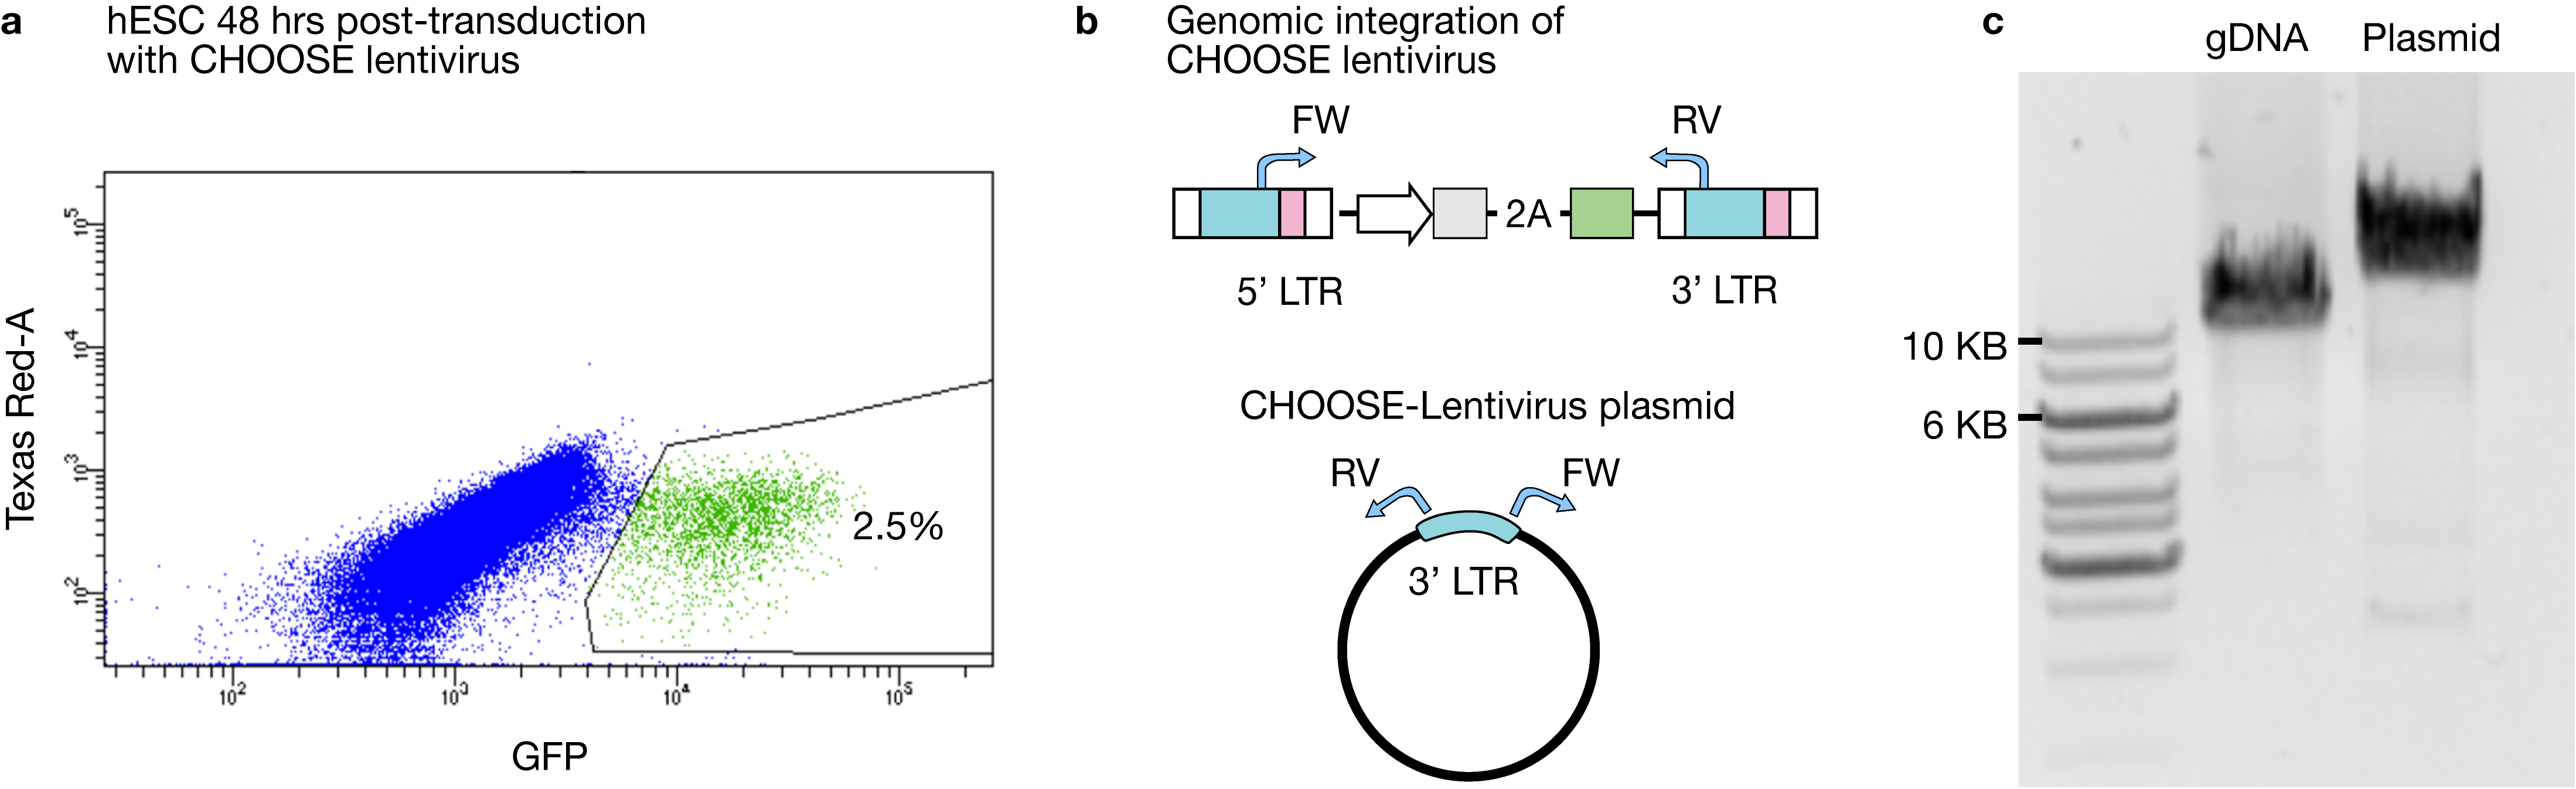
\includegraphics[width=\textwidth]{figures/asd/Figure_S2}
    \label{fig:asdS2}
    \caption{\textbf{Infection and integration of CHOOSE lentivirus on hESCs.} 
    a, Infection rate of CHOOSE lentivirus on hESCs determined by flow-cytometry. Infected cells are positive for GFP. b, Top diagram shows the duplication of the dual-sgRNA cassette after the lentiviral integration into the host genome. FW and RV are paired primers used to demonstrate the successful integration of the lentivirus. The primers amplify specific regions of the genomic DNA extracted from lentivirus-infected hESCs, and the lentiviral plasmid. c, Gel electrophoresis analysis showing 12 kb and 13 kb bands detected from gDNA and plasmid respectively.}
\end{figure}


\begin{figure}[h!]
    \centering
	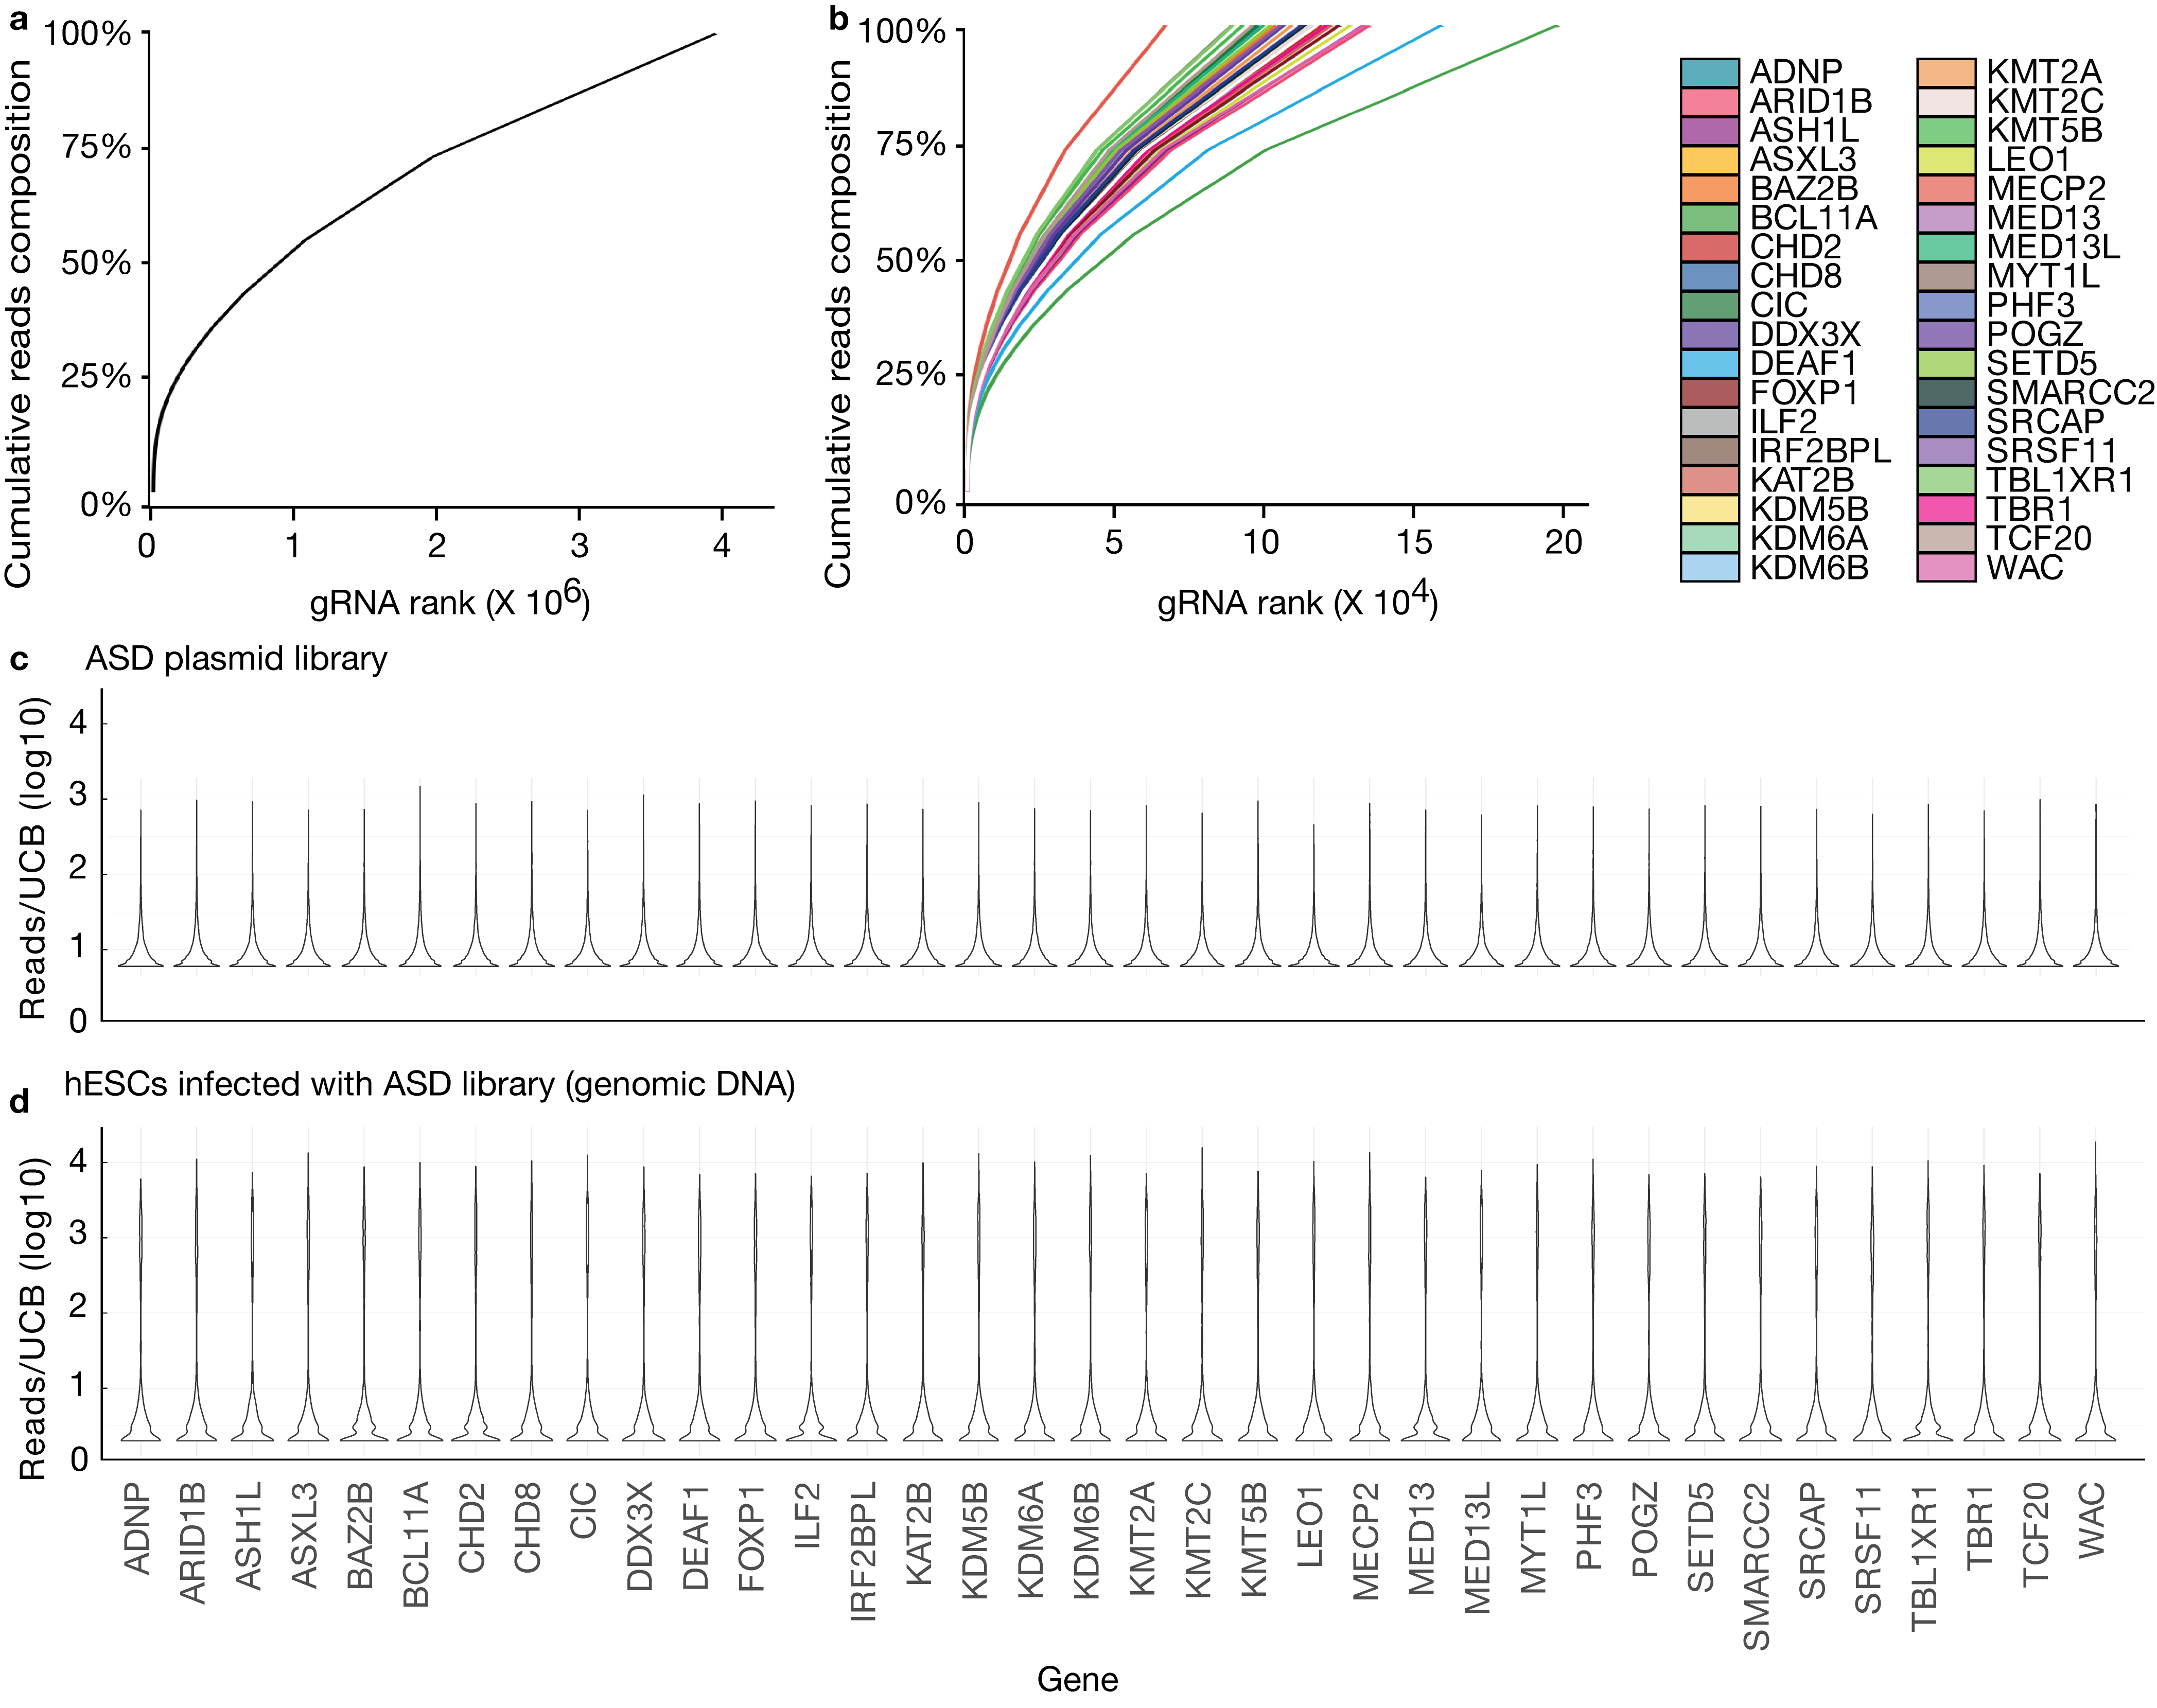
\includegraphics[width=\textwidth]{figures/asd/Figure_S3}
    \label{fig:asdS3}
    \caption{\textbf{Clone barcode diversity of the CHOOSE library.} 
    a, Plot shows cumulative fraction of uniquely barcoded gRNA cassettes from the CHOOSE ASD plasmid library. b, Plot shows cumulative fraction of uniquely barcoded gRNA cassettes separated by each target gene from the plasmid library. c,d, Reads distribution for each barcoded gNRA cassette from the  plasmid library (c) and from genomic DNA (d) extracted from the hESCs infected by lentivirus. UCB, unique clone barcode.}
\end{figure}



\begin{figure}[h!]
    \centering
	\includegraphics[width=\textwidth]{figures/asd/Figure_S4}
    \label{fig:asdS4}
    \caption{\textbf{Generation of cerebral organoids using the CHOOSE system.} 
    a, Schematic showing the protocol used for generating cerebral organoids. 4-OHT was added to induce eCas9 expression at day 5. A short 3-day CHIR treatment was applied from day 12-14. Culture medium was switched to Brainphys after day 60 for advanced neuronal maturation. Tissues are collected at day 120 and subjected to scRNA-seq assays. b, ESCs were infected by lentivirus and GFP positive cells were collected to make EBs. Microscopic images show the overall morphology and GFP expression of brain organoids overtime. Top, bright-field; Bottom, GFP fluorescence. c. Immunohistochemical staining of cerebral organoids at day 24. GFP labels cells infected with lentivirus and Tomato is a reporter for eCas9 expression. SOX2 is a marker for progenitor cells. FOXG1 is a marker for tissues with telencephalon identity.}
\end{figure}



\begin{figure}[h!]
    \centering
	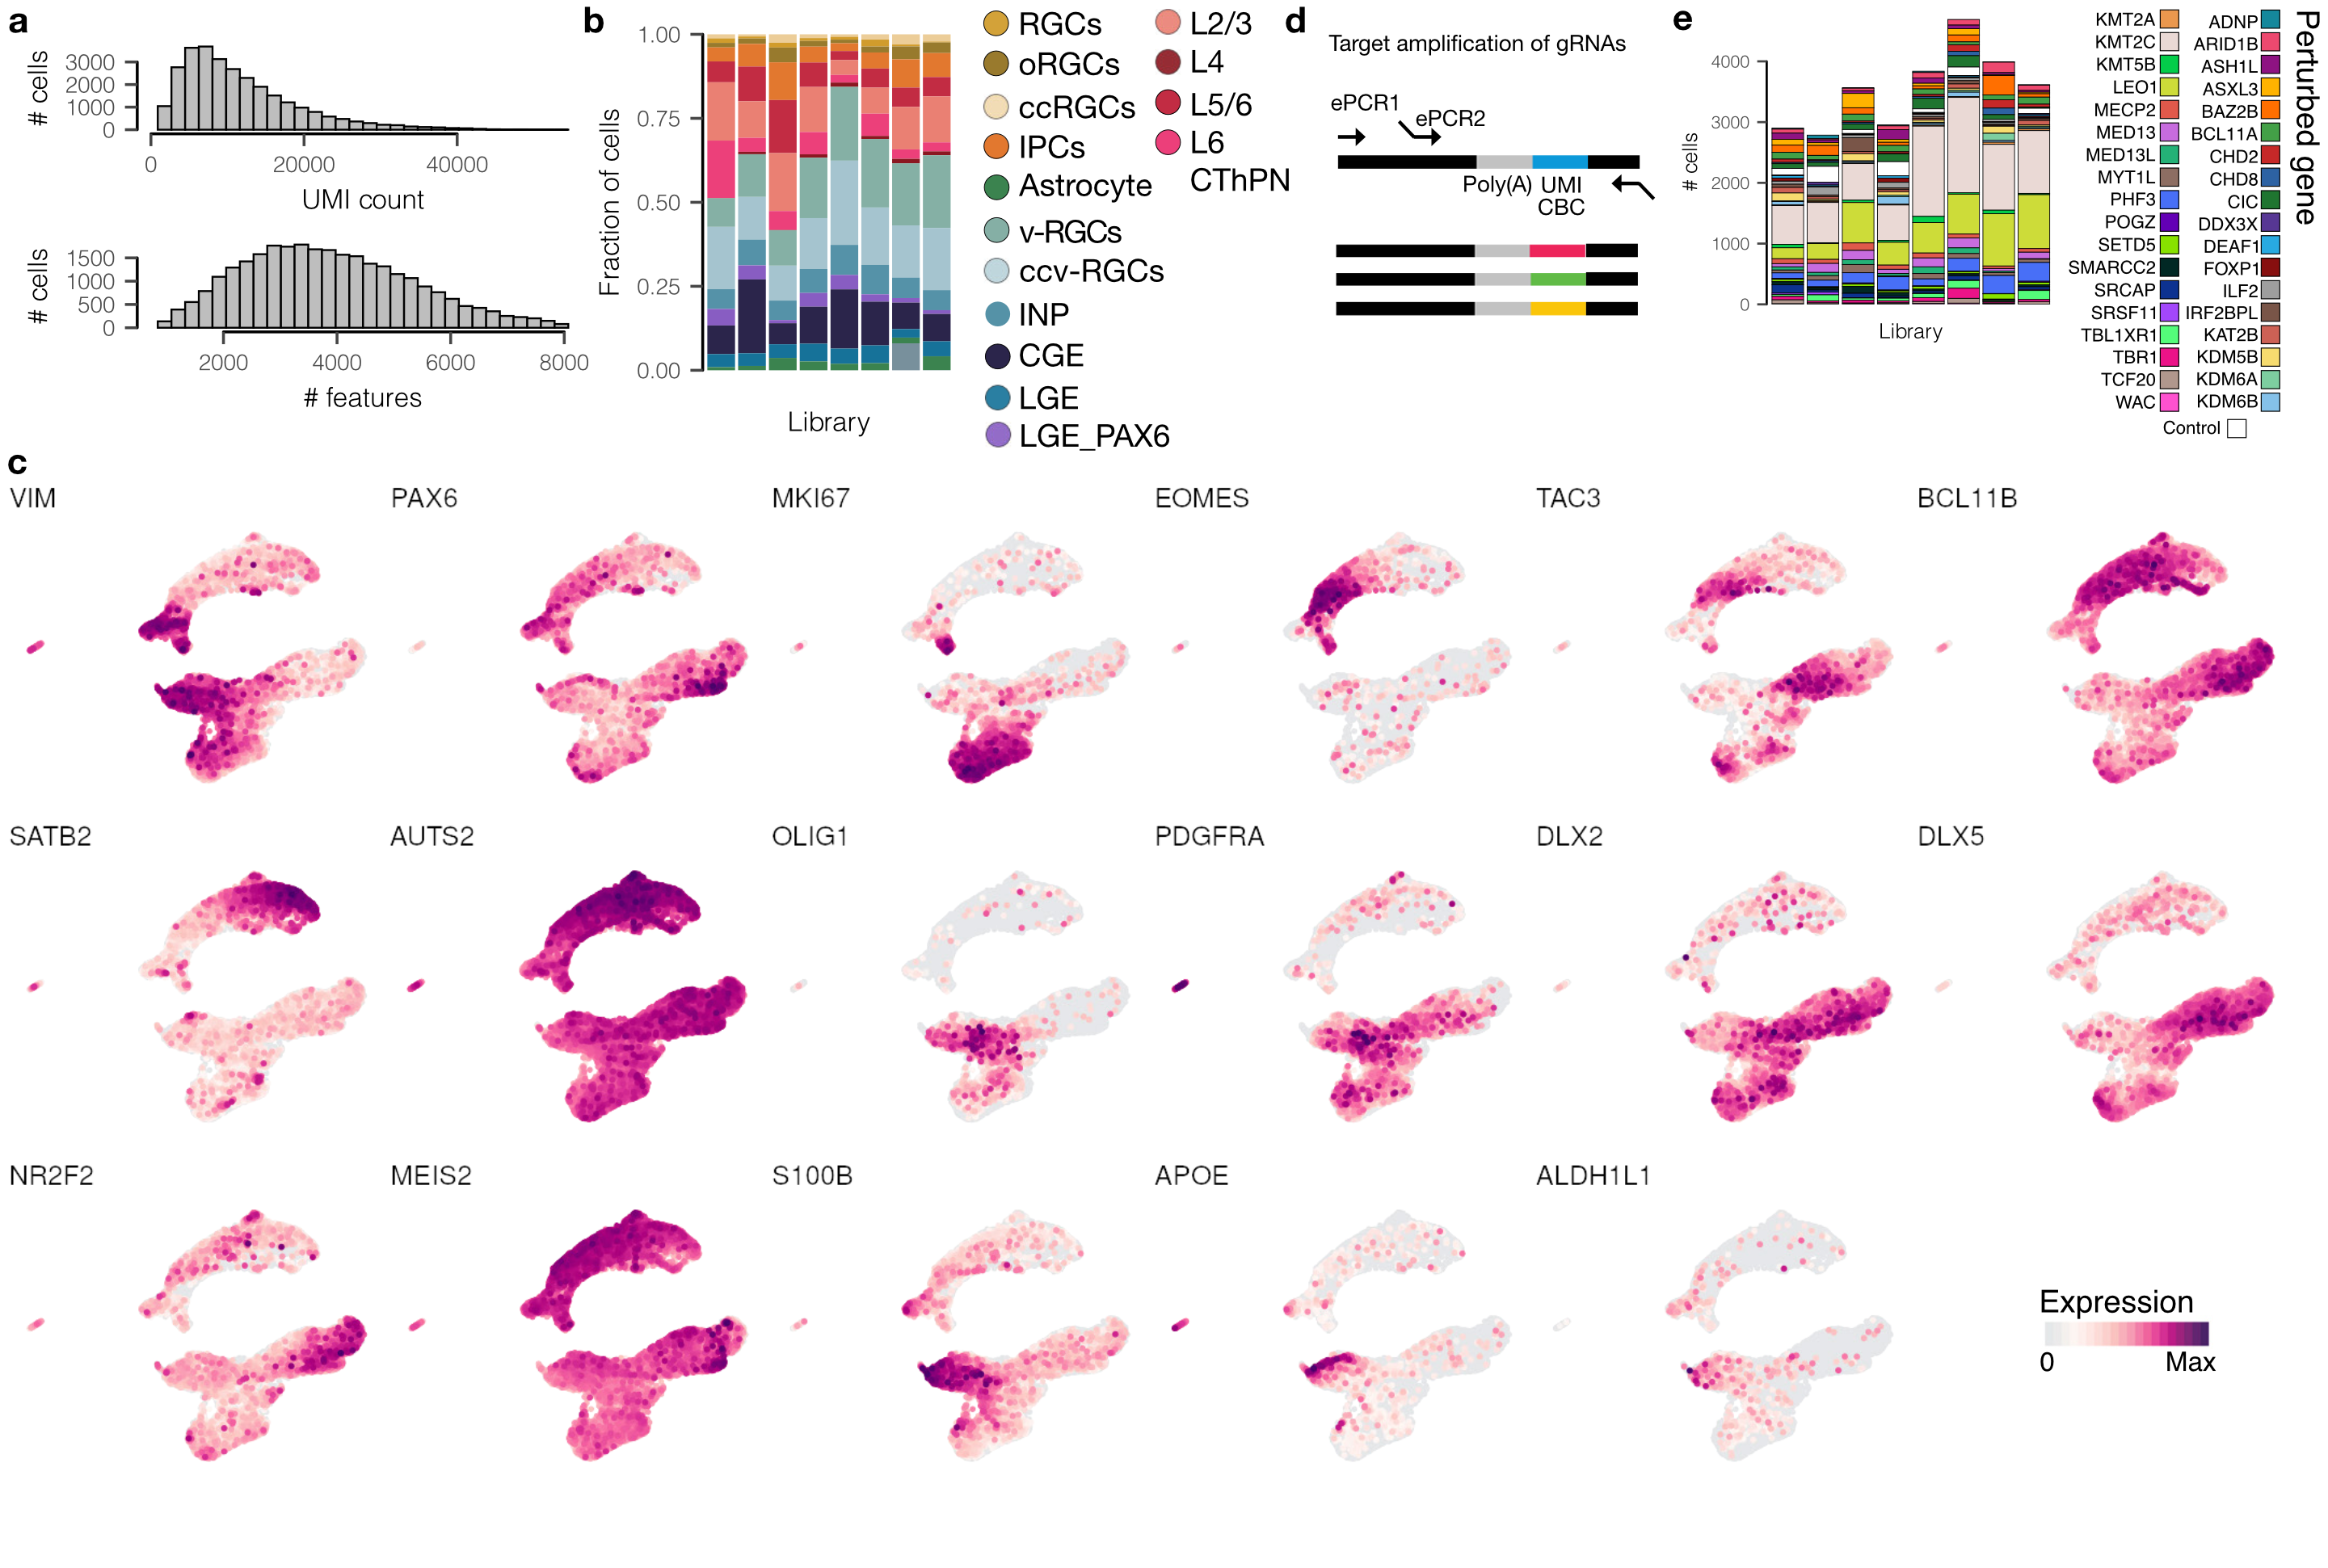
\includegraphics[width=\textwidth]{figures/asd/Figure_S5}
    \label{fig:asdS5}
    \caption{\textbf{Cell type and gRNA composition of scRNA-seq libraries.} 
    a, Histograms showing UMI count and number of detected features in the QC-controlled scRNA-seq dataset. b, Cell type compositions for each 10X library. In total 8 libraries (31 cerebral organoids) are processed and sequenced. c, Feature plots showing expression of marker genes on a UMAP embedding. d, Target amplification with hemi-nested emulsion PCR (ePCR) used to recover gRNA information. e, Bar plot shows numbers of recovered cells with assigned gRNAs for each library.}
\end{figure}



\begin{figure}[h!]
    \centering
	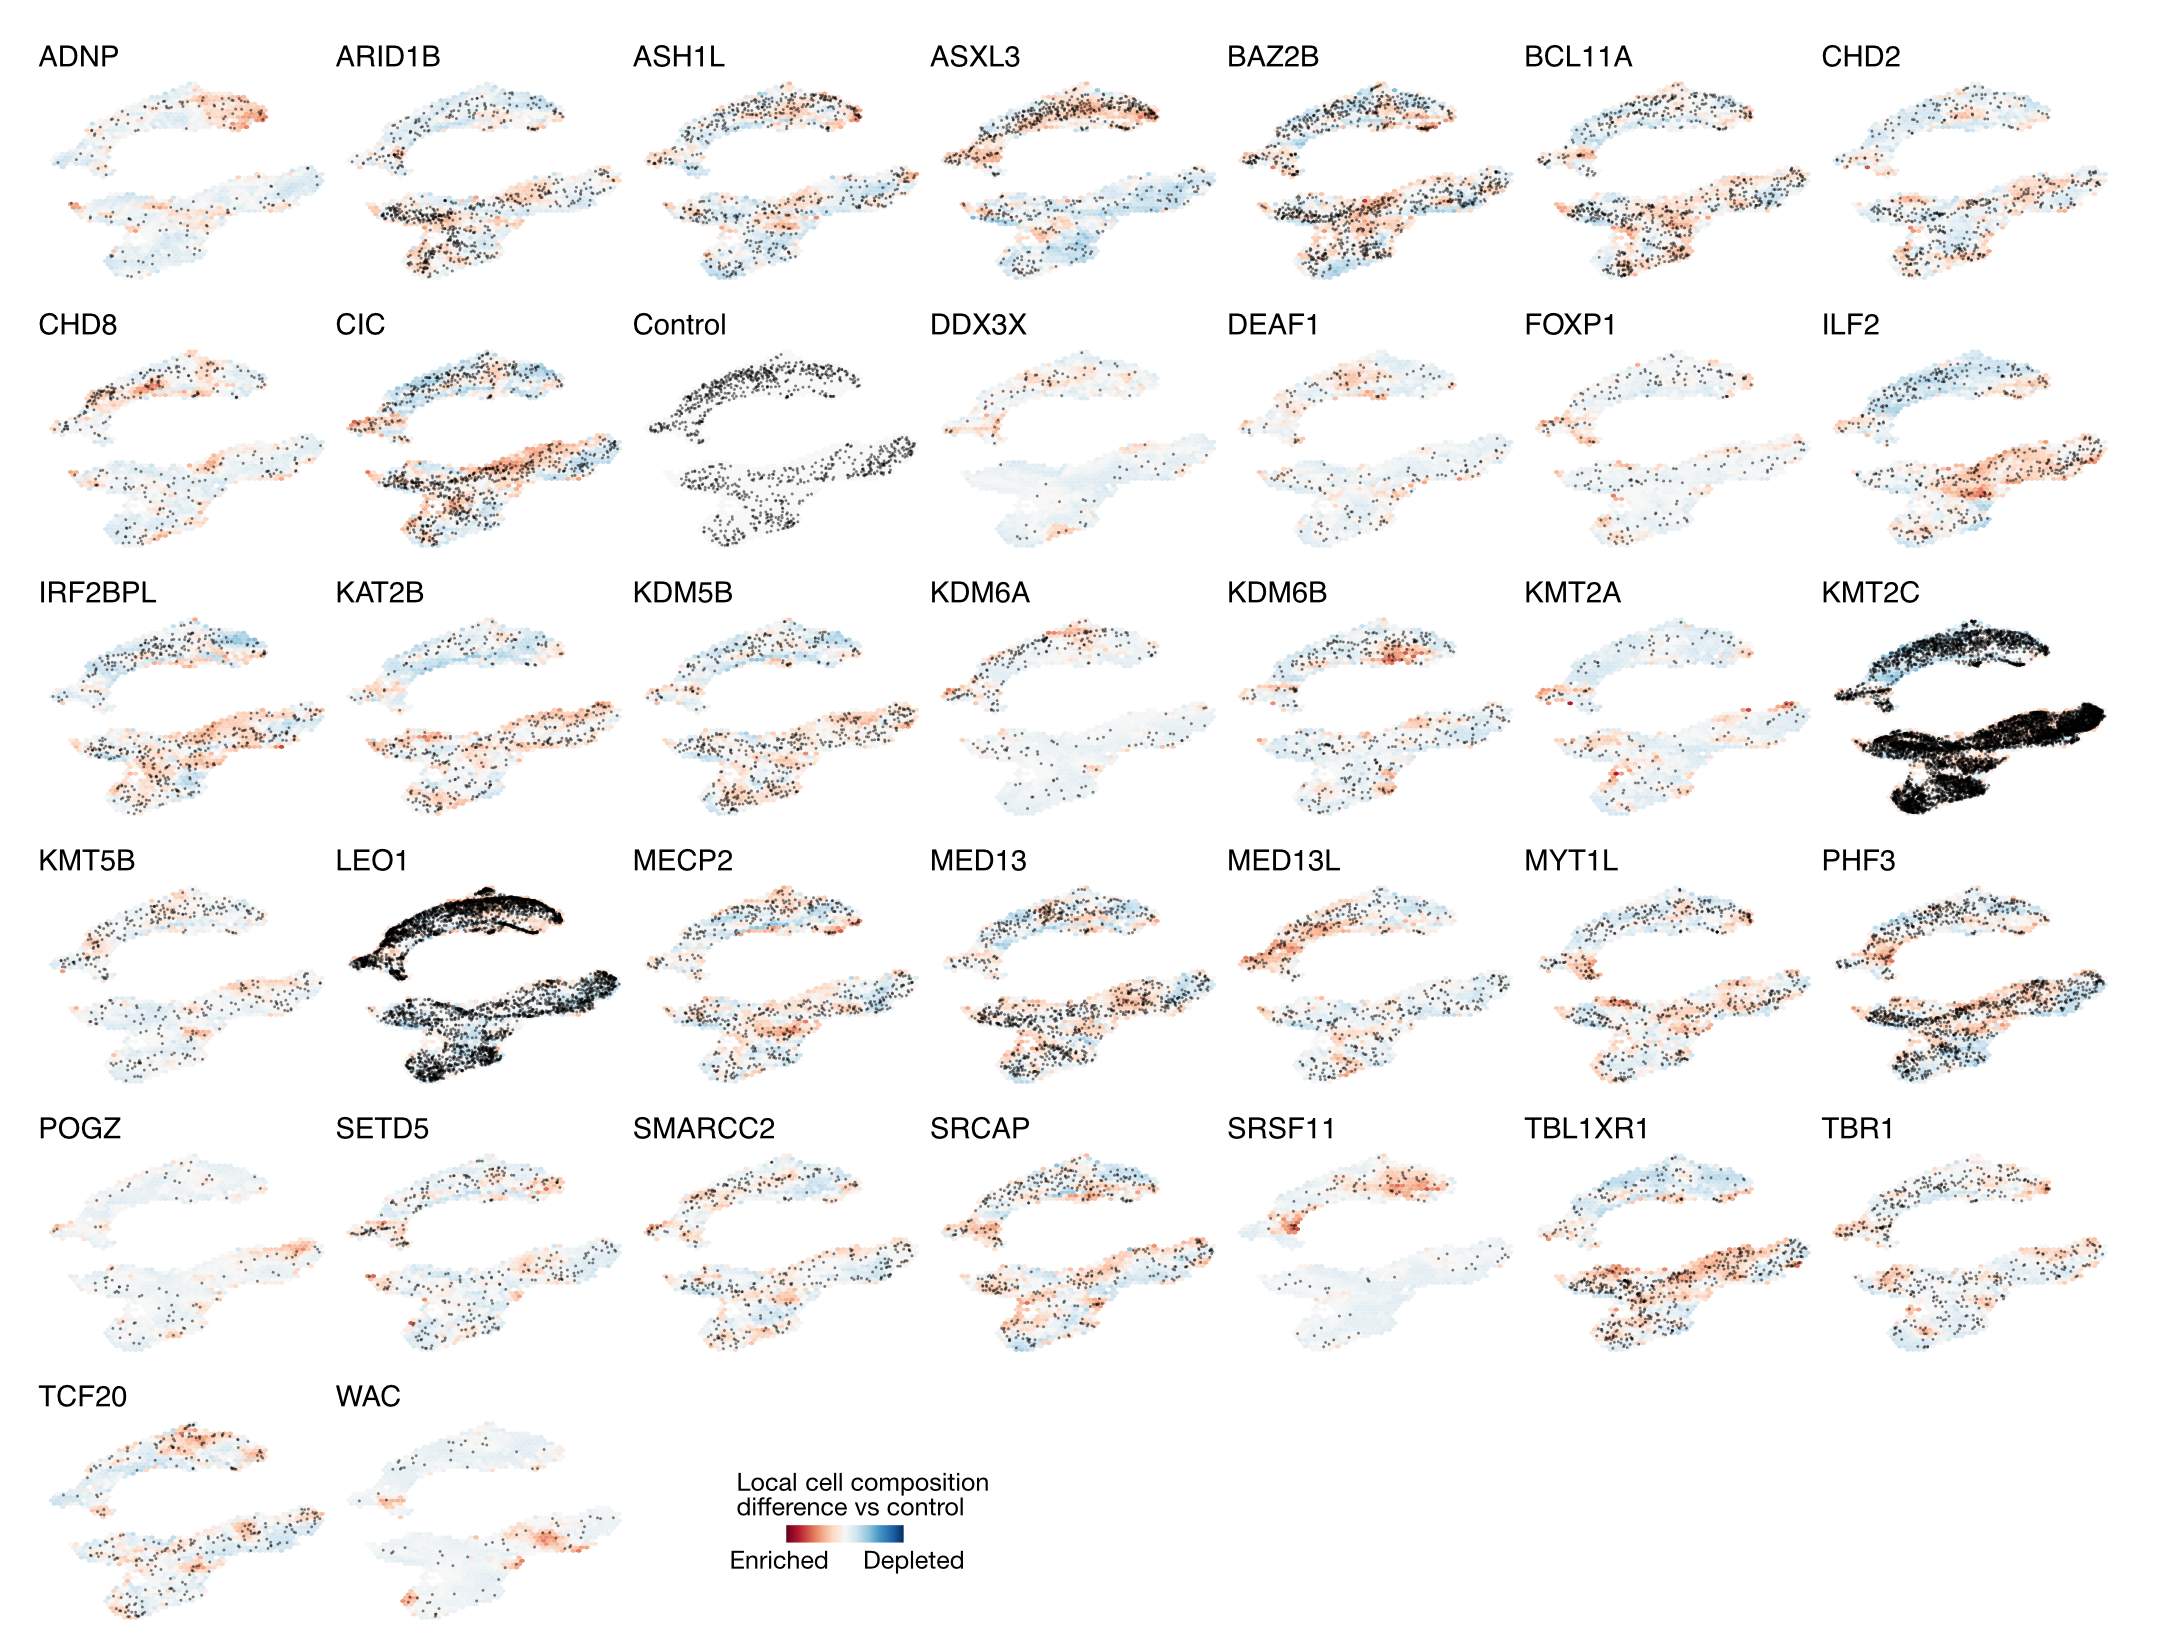
\includegraphics[width=\textwidth]{figures/asd/Figure_S6}
    \label{fig:asdS6}
    \caption{\textbf{Cell type compositional changes caused by ASD gene perturbations.} 
    UMAP embeddings show single cell distribution for each perturbed gene. Local cell composition differences of perturbation versus control indicated by red (enrichment) or blue (depletion).}
\end{figure}



\begin{figure}[h!]
    \centering
	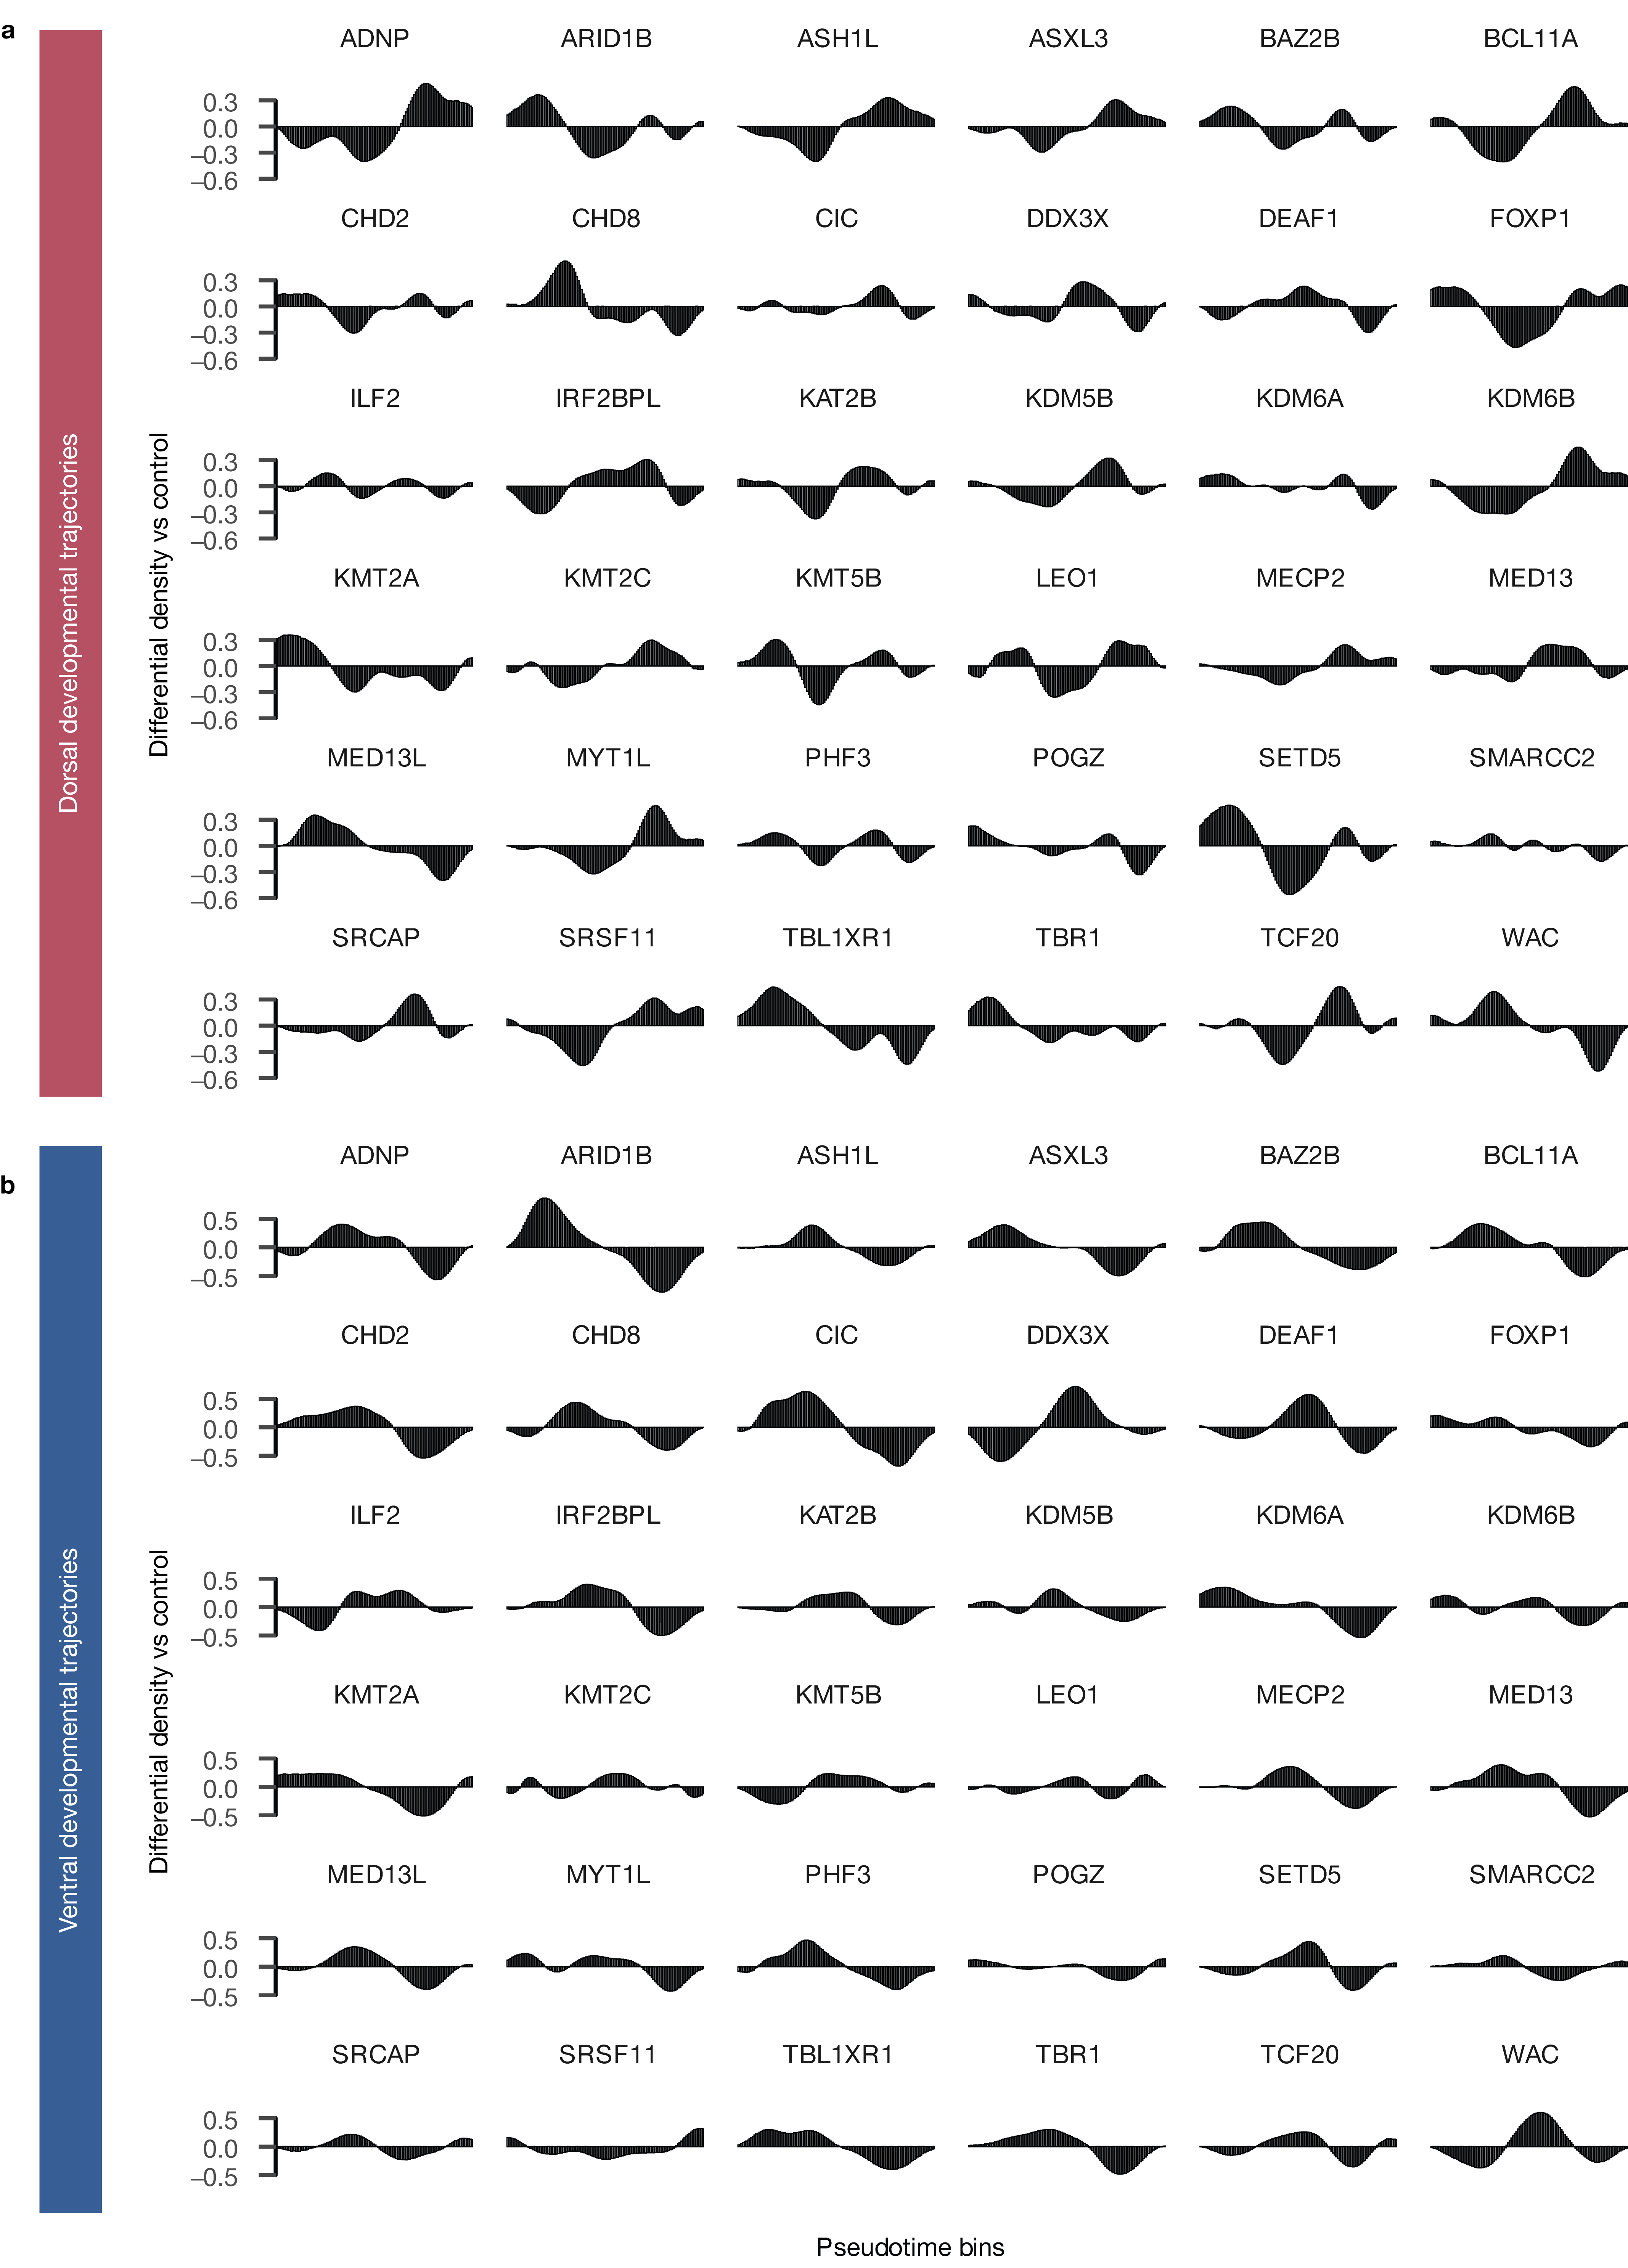
\includegraphics[width=\textwidth]{figures/asd/Figure_S7}
    \label{fig:asdS7}
    \caption{\textbf{Developmental process-specific effects of ASD gene perturbations.} 
    Differential cell density along a binned pseudo-temporal axis of perturbations versus control for each gene perturbation. Plots are separated by dorsal and ventral telencephalon trajectories.}
\end{figure}



\begin{figure}[h!]
    \centering
	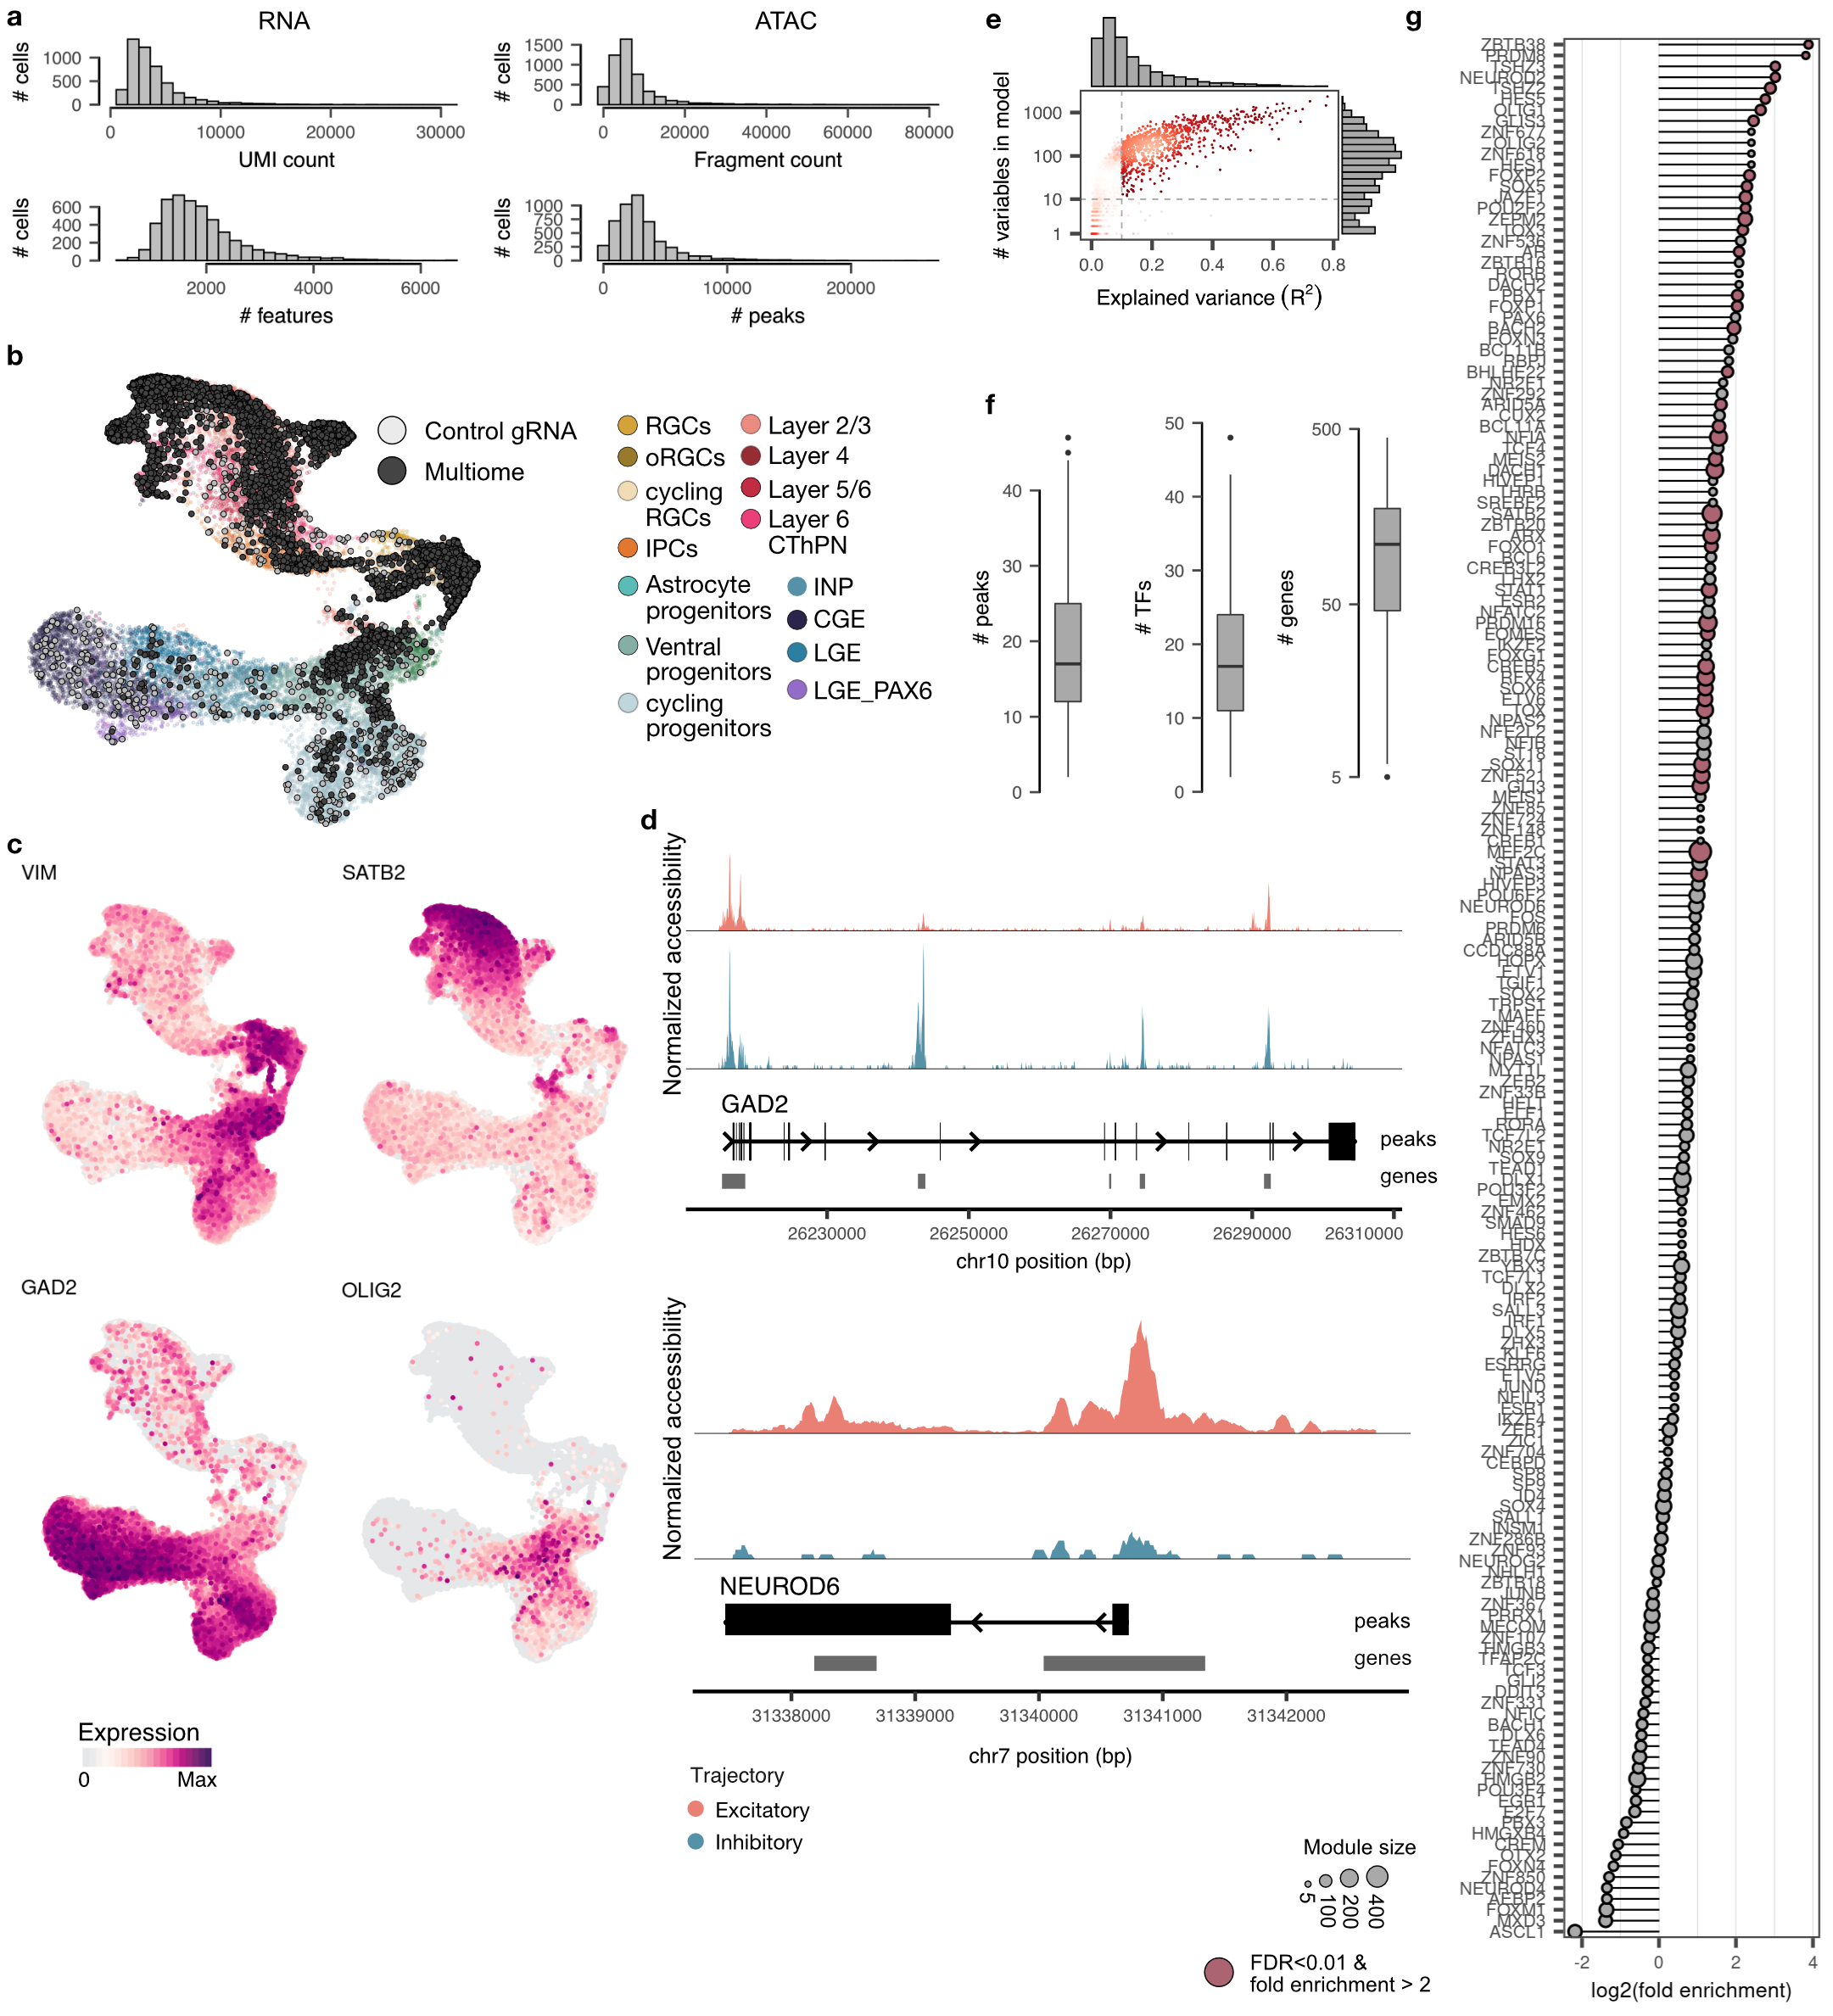
\includegraphics[width=\textwidth]{figures/asd/Figure_S8}
    \label{fig:asdS8}
    \caption{\textbf{Quality control and GRN inference from the single-cell multiome dataset.} 
    a, Histograms showing UMI count and number of detected features for RNA as well as fragment count and number of detected peaks for ATAC. b, UMAP embedding showing multiome data (black) integrated with the CHOOSE dataset. Multiome data were used in conjunction with the control cells from the CHOOSE dataset (grey) to infer the GRN with Pando. c, Feature plots showing expression of marker genes on the UMAP embedding. d, Genomic tracks showing accessible peaks in the proximity of GAD2 (ventral marker) and NEUROD6 (dorsal marker). e, Density scatter plot histograms showing the distributions of explained variance (x) and number of variables (y) in the fitted models for GRN construction. Dashed lines indicate the thresholds used for model selection. f, Boxplots showing the distribution of peaks (left) and TFs assigned per gene (middle), and number of genes assigned per TF (right) in the inferred GRN. g, Lolliplot showing the enrichment of ASD-associated genes from SFARI in inferred TF modules. Red color indicates an FDR-corrected Fisher-test p-value of <0.01. Dot size indicates the total number of genes in the module.}
\end{figure}



\begin{figure}[h!]
    \centering
	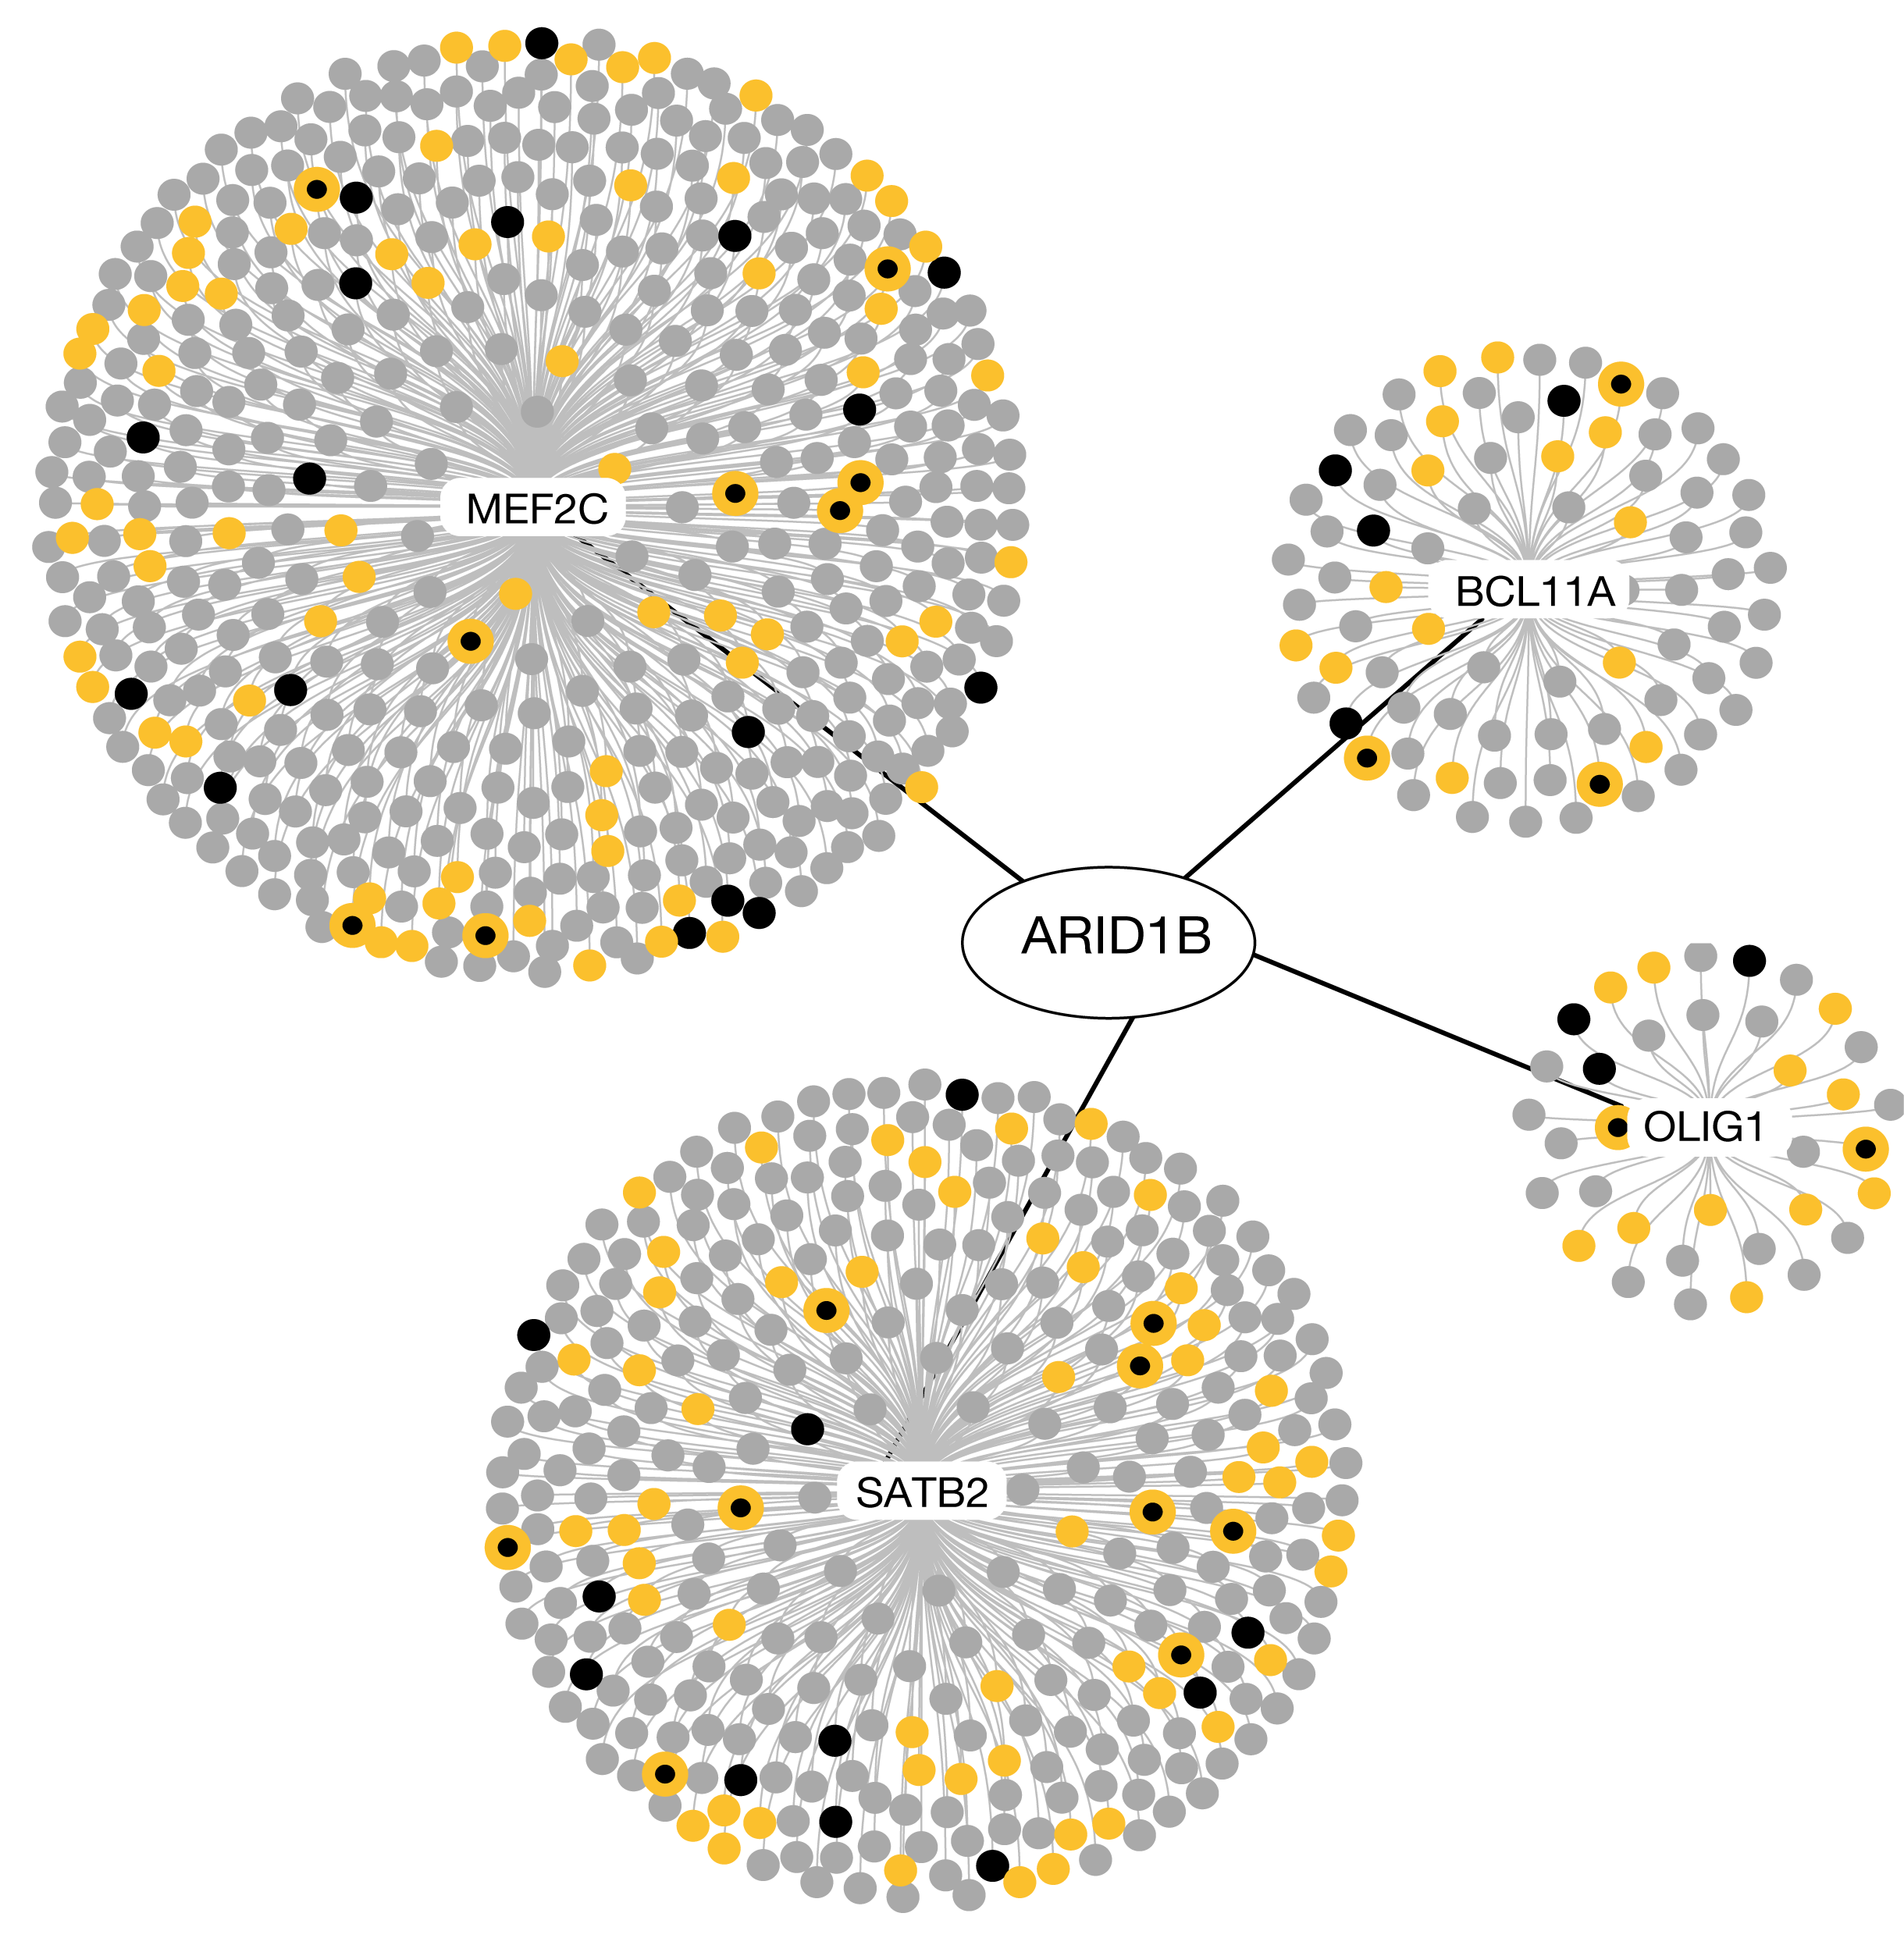
\includegraphics[width=\textwidth]{figures/asd/Figure_S9}
    \label{fig:asdS9}
    \caption{\textbf{ARID1B perturbation-induced DEGs are enriched in the OLIG1 regulatory module.}  
    Graph representation of MEF2C, BCL11A, SATB2, and OLIG1 TF modules, which are most strongly enriched in ARID1B DEG (Fisher exact test p-value < 0.01, top 4 odds ratio). The targets highlighted in yellow are SFARI genes, and the targets highlighted in black are TF modules enriched in SFARI genes. }
\end{figure}



\begin{figure}[h!]
    \centering
	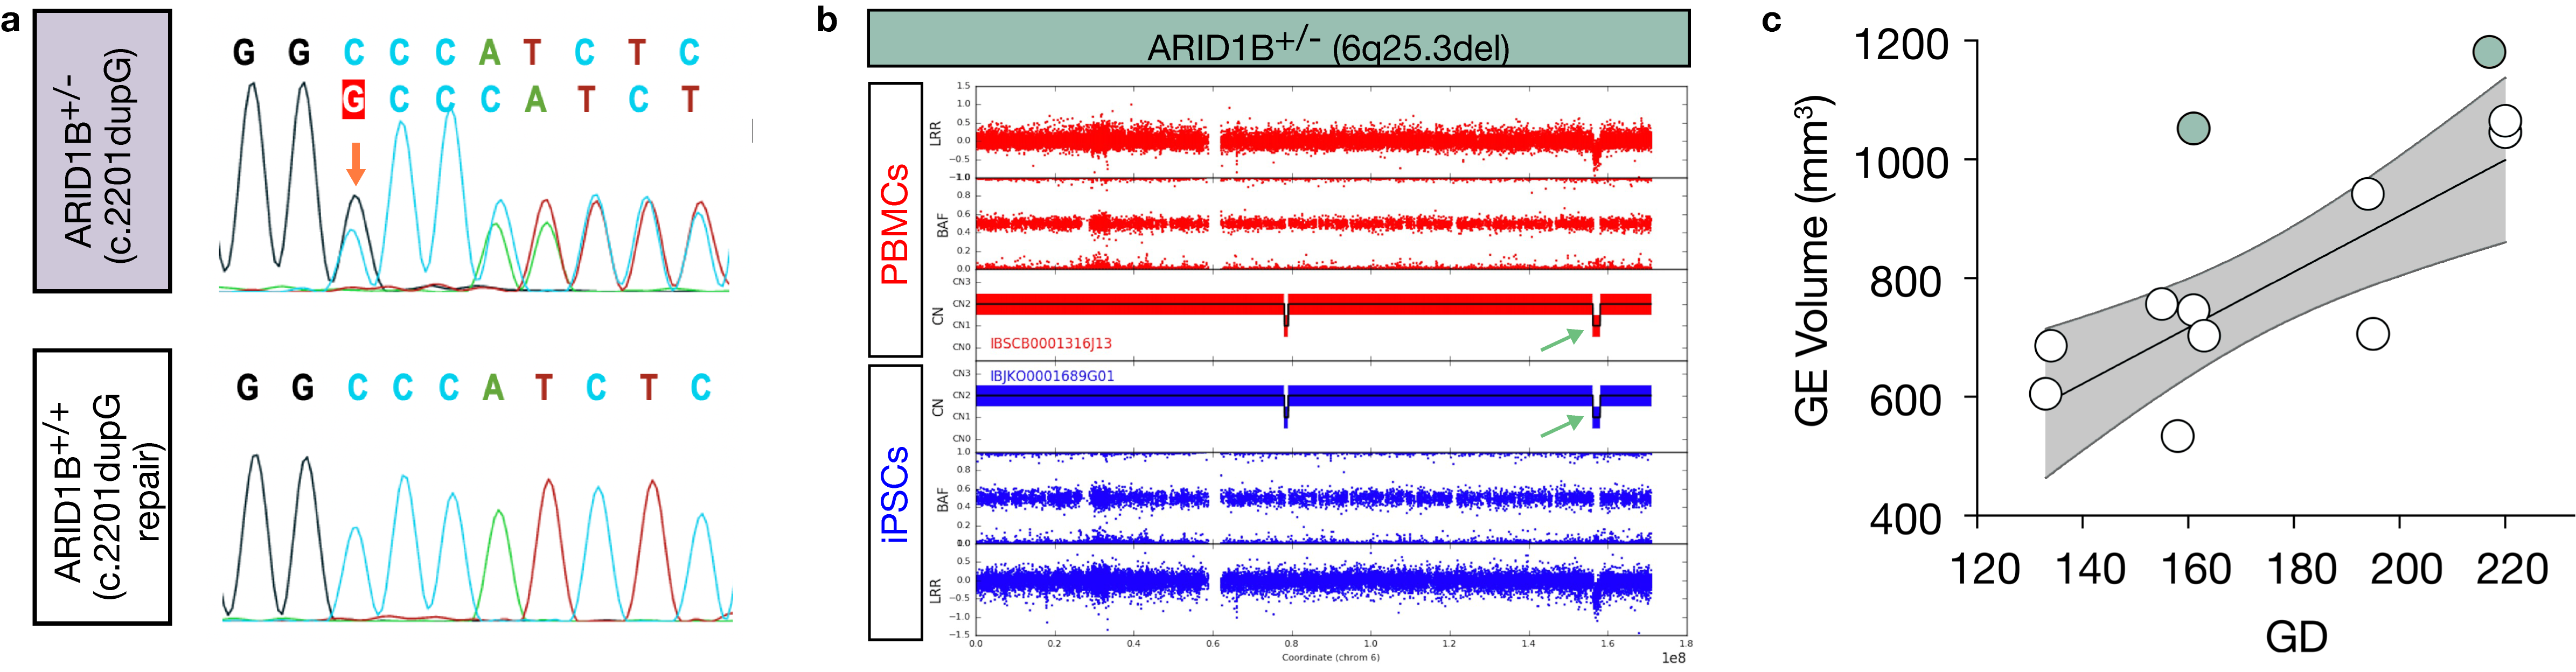
\includegraphics[width=\textwidth]{figures/asd/Figure_S10}
    \label{fig:asdS10}
    \caption{\textbf{An ARID1B patient had enlarged ganglionic eminence.}  
    a, Top, sanger sequencing showing a duplication mutation (red arrow) identified in one of the alleles of patient 1. Bottom, sanger sequencing showing the mutation was repaired and this cell line is used as an isogenic control. Sequencing was done on fragments amplified from genomic DNA extracted from the two iPSC lines.  b, SNP array genotyping of PBMCs and iPSCs from patient 2 shows a microdeletion (dark green arrow) identified on chromosome 6. c, Dot plot of the GE (LGE and CGE) volume of patient 2 (dark green circles) at two gestation stages. The white circles represent age-matched controls. A simple linear regression model was constructed using data from all controls. The gray area represents the 95\% confidence interval.}
\end{figure}


\clearpage

\newpage
\thispagestyle{empty}
\
\newpage
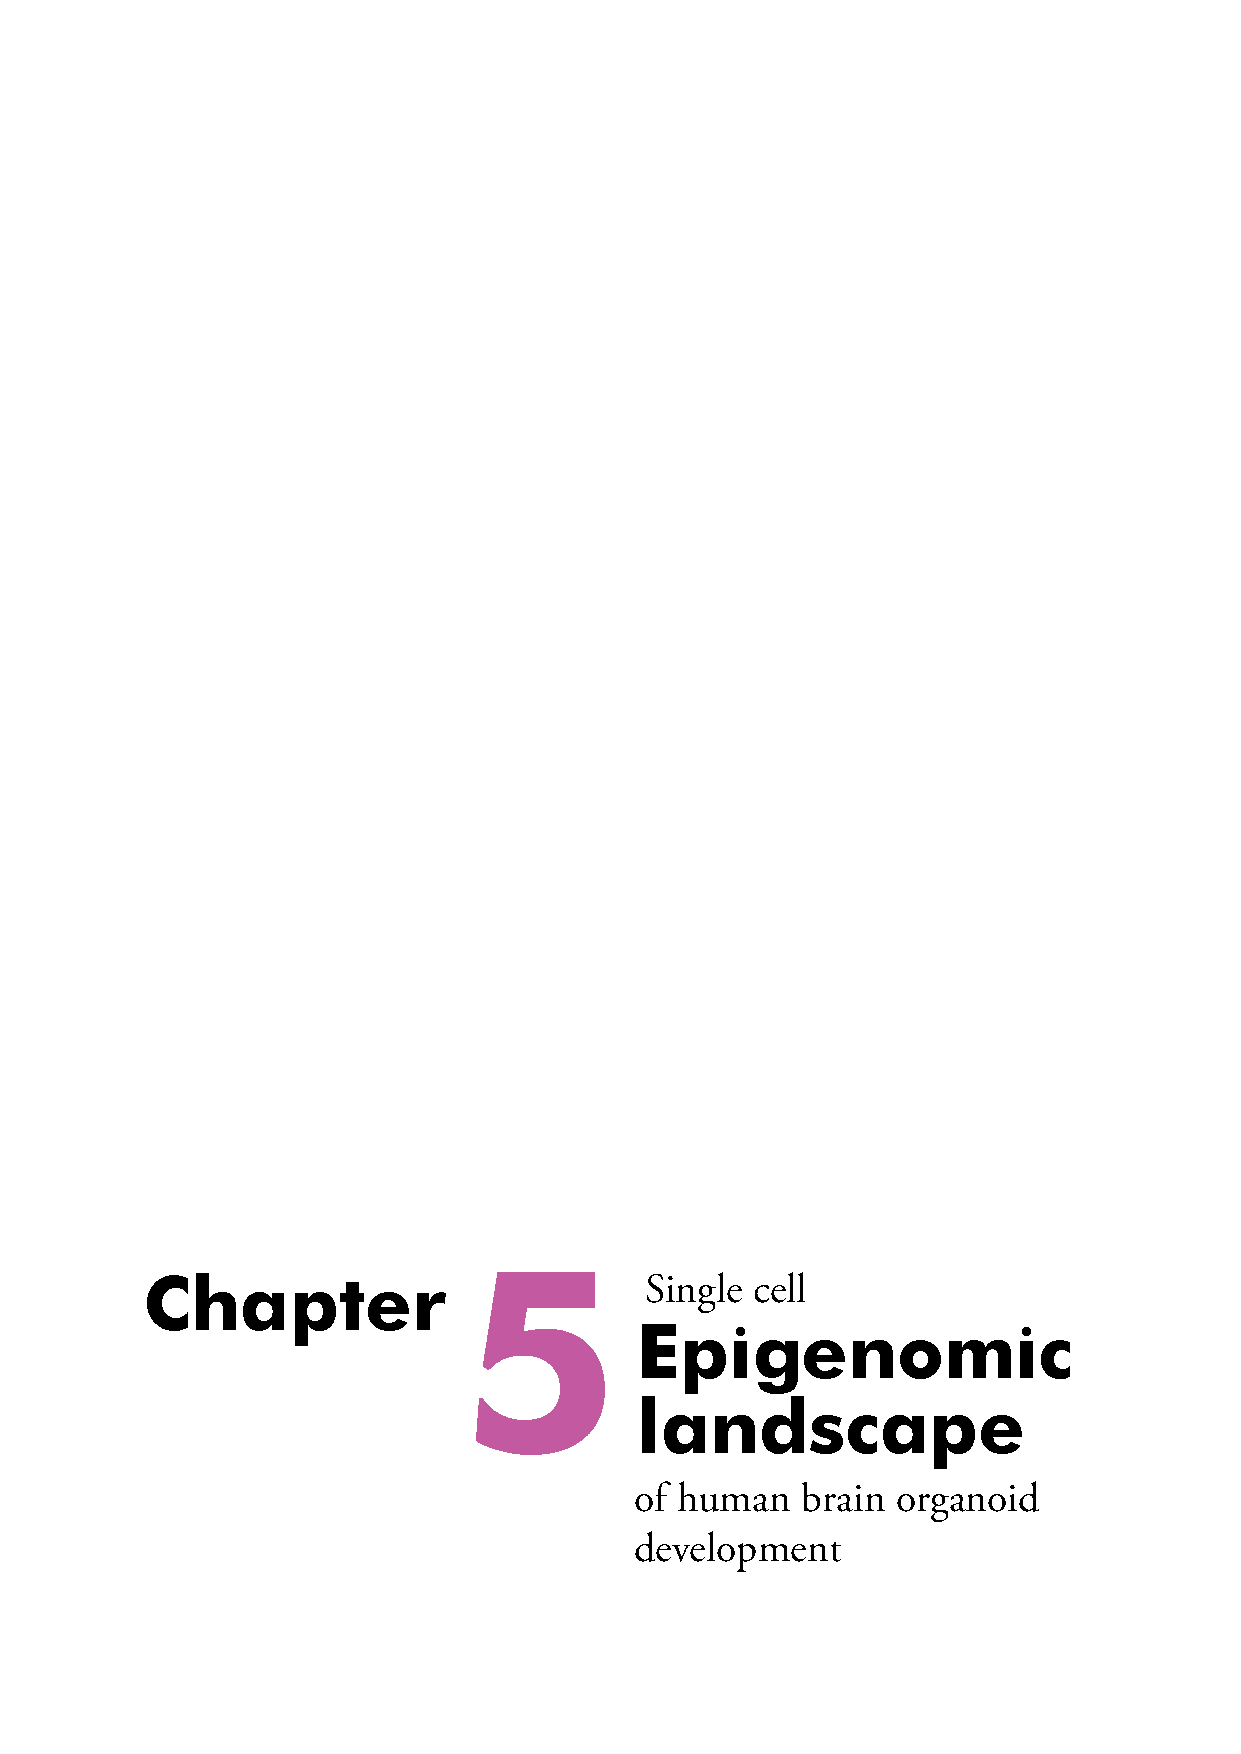
\includepdf[fitpaper=true, pages=-]{pdfs/chapter_5.pdf}

\thispagestyle{plain}
\section{Single-cell epigenomic landscape of human brain organoid development}
\markboth{Single-cell epigenomic landscape of human brain organoid development}{}

\vspace{0.5cm}

Chapter 5 is a study entitled 'Single-cell epigenomic landscape of human brain organoid development', which is currently \textit{in preparation}. I contributed major parts of the computational analyses for the presented scRNA-seq and scCut\&Tag data, including annotation, multi-modal integration, trajectory inference and differential expression analysis.

\vspace{1cm}

\noindent
{\large\textsc{Authors}}

\noindent
Fides Zenk\textsuperscript{1$*$}, 
Jonas Simon Fleck\textsuperscript{1$*$}, 
Sophie Martina Johanna Jansen\textsuperscript{1}, 
Bijan Kashanian\textsuperscript{1}, 
Benedikt Eisinger\textsuperscript{1}, 
Malgorzata Santel\textsuperscript{1}, 
J Gray Camp\textsuperscript{2,3}
Barbara Treutlein\textsuperscript{1}

\vspace{0.5cm}

\noindent
$\ast$ Equal contribution

\vspace{1cm}

\noindent
{\large\textsc{Affiliations}}

\noindent
\textsuperscript{1} Department of Biosystems Science and Engineering, ETH Zürich, Basel, Switzerland\\
\textsuperscript{2} University of Basel, Basel, Switzerland\\
\textsuperscript{3} Roche Institute for Translational Bioengineering (ITB), Roche Pharma Research and Early Development, Roche Innovation Center Basel, Switzerland

\vspace{1cm}

\noindent
{\large\textsc{Author contributions}}

\noindent
F.Z. generated organoids used in this study, with support from B.K. and M.S.. M.S. helped with iPS cell culture. F.Z generated all single-cell transcriptome and single-cell Cut\&Tag datasets with support from S.J.. F.Z. performed the drug-treatment, bulk Cut\&Tag and Western Blot experiments. F.Z. performed immunofluorescence experiments with support from B.E.. J.S.F. performed the analysis of the scRNA-seq/scATAC-seq developmental time course with support from F.Z.. J.S.F. analyzed the drug treatment scRNA-seq and bulk Cut\&Tag data with support from F.Z.. F.Z., B.T. and J.G.C. designed the study and F.Z., J.S.F., B.T. and J.G.C. wrote the manuscript.

\clearpage

\subsection{Abstract}

The cell type diversity of the human body originates from just one single totipotent cell. How the different cell types emerge from the same genomic sequence and how they maintain their identities throughout development is still an open question in biology. Epigenetic modifications that can direct the activity of genes and regulatory elements during development play an important role in the process of cell identity decisions.
Here, we explore how brain development and in particular, the differentiation of progenitor cells into different neuronal and glial cell types is regulated by epigenetic mechanisms. We use brain organoids to model the earliest events of cell fate acquisition in the developing brain and apply single-cell epigenetic profiling of histone modifications at various stages of brain organoid development. We use this data to reconstruct the epigenetic trajectory governing cell fate acquisition. We find that switching of epigenetic modifications can precede and predict the activation of important brain region-specific transcription factors. Further, we show that perturbation of histone modifiers during neuroectoderm establishment disrupts fate decisions and leads to aberrant cell fate acquisition. In summary, we provide the first comprehensive single-cell atlas of histone modifications during human brain organoid development, which will serve as a reference to understand early fate decisions but also neurodevelopmental diseases associated with chromatin regulators.


\subsection{Main}

During development and differentiation, cells undergo remarkable cell fate transitions starting from pluripotent cells and progenitors to give rise to all major cell types of the body. During these transitions, developmental plasticity becomes increasingly restricted until the cells stop dividing and acquire their terminal fate. Despite recent progress in epigenetics and reprogramming, the question of how cells acquire and maintain their identity on a global scale is still elusive. 

\begin{figure}[b!]
    \centering
	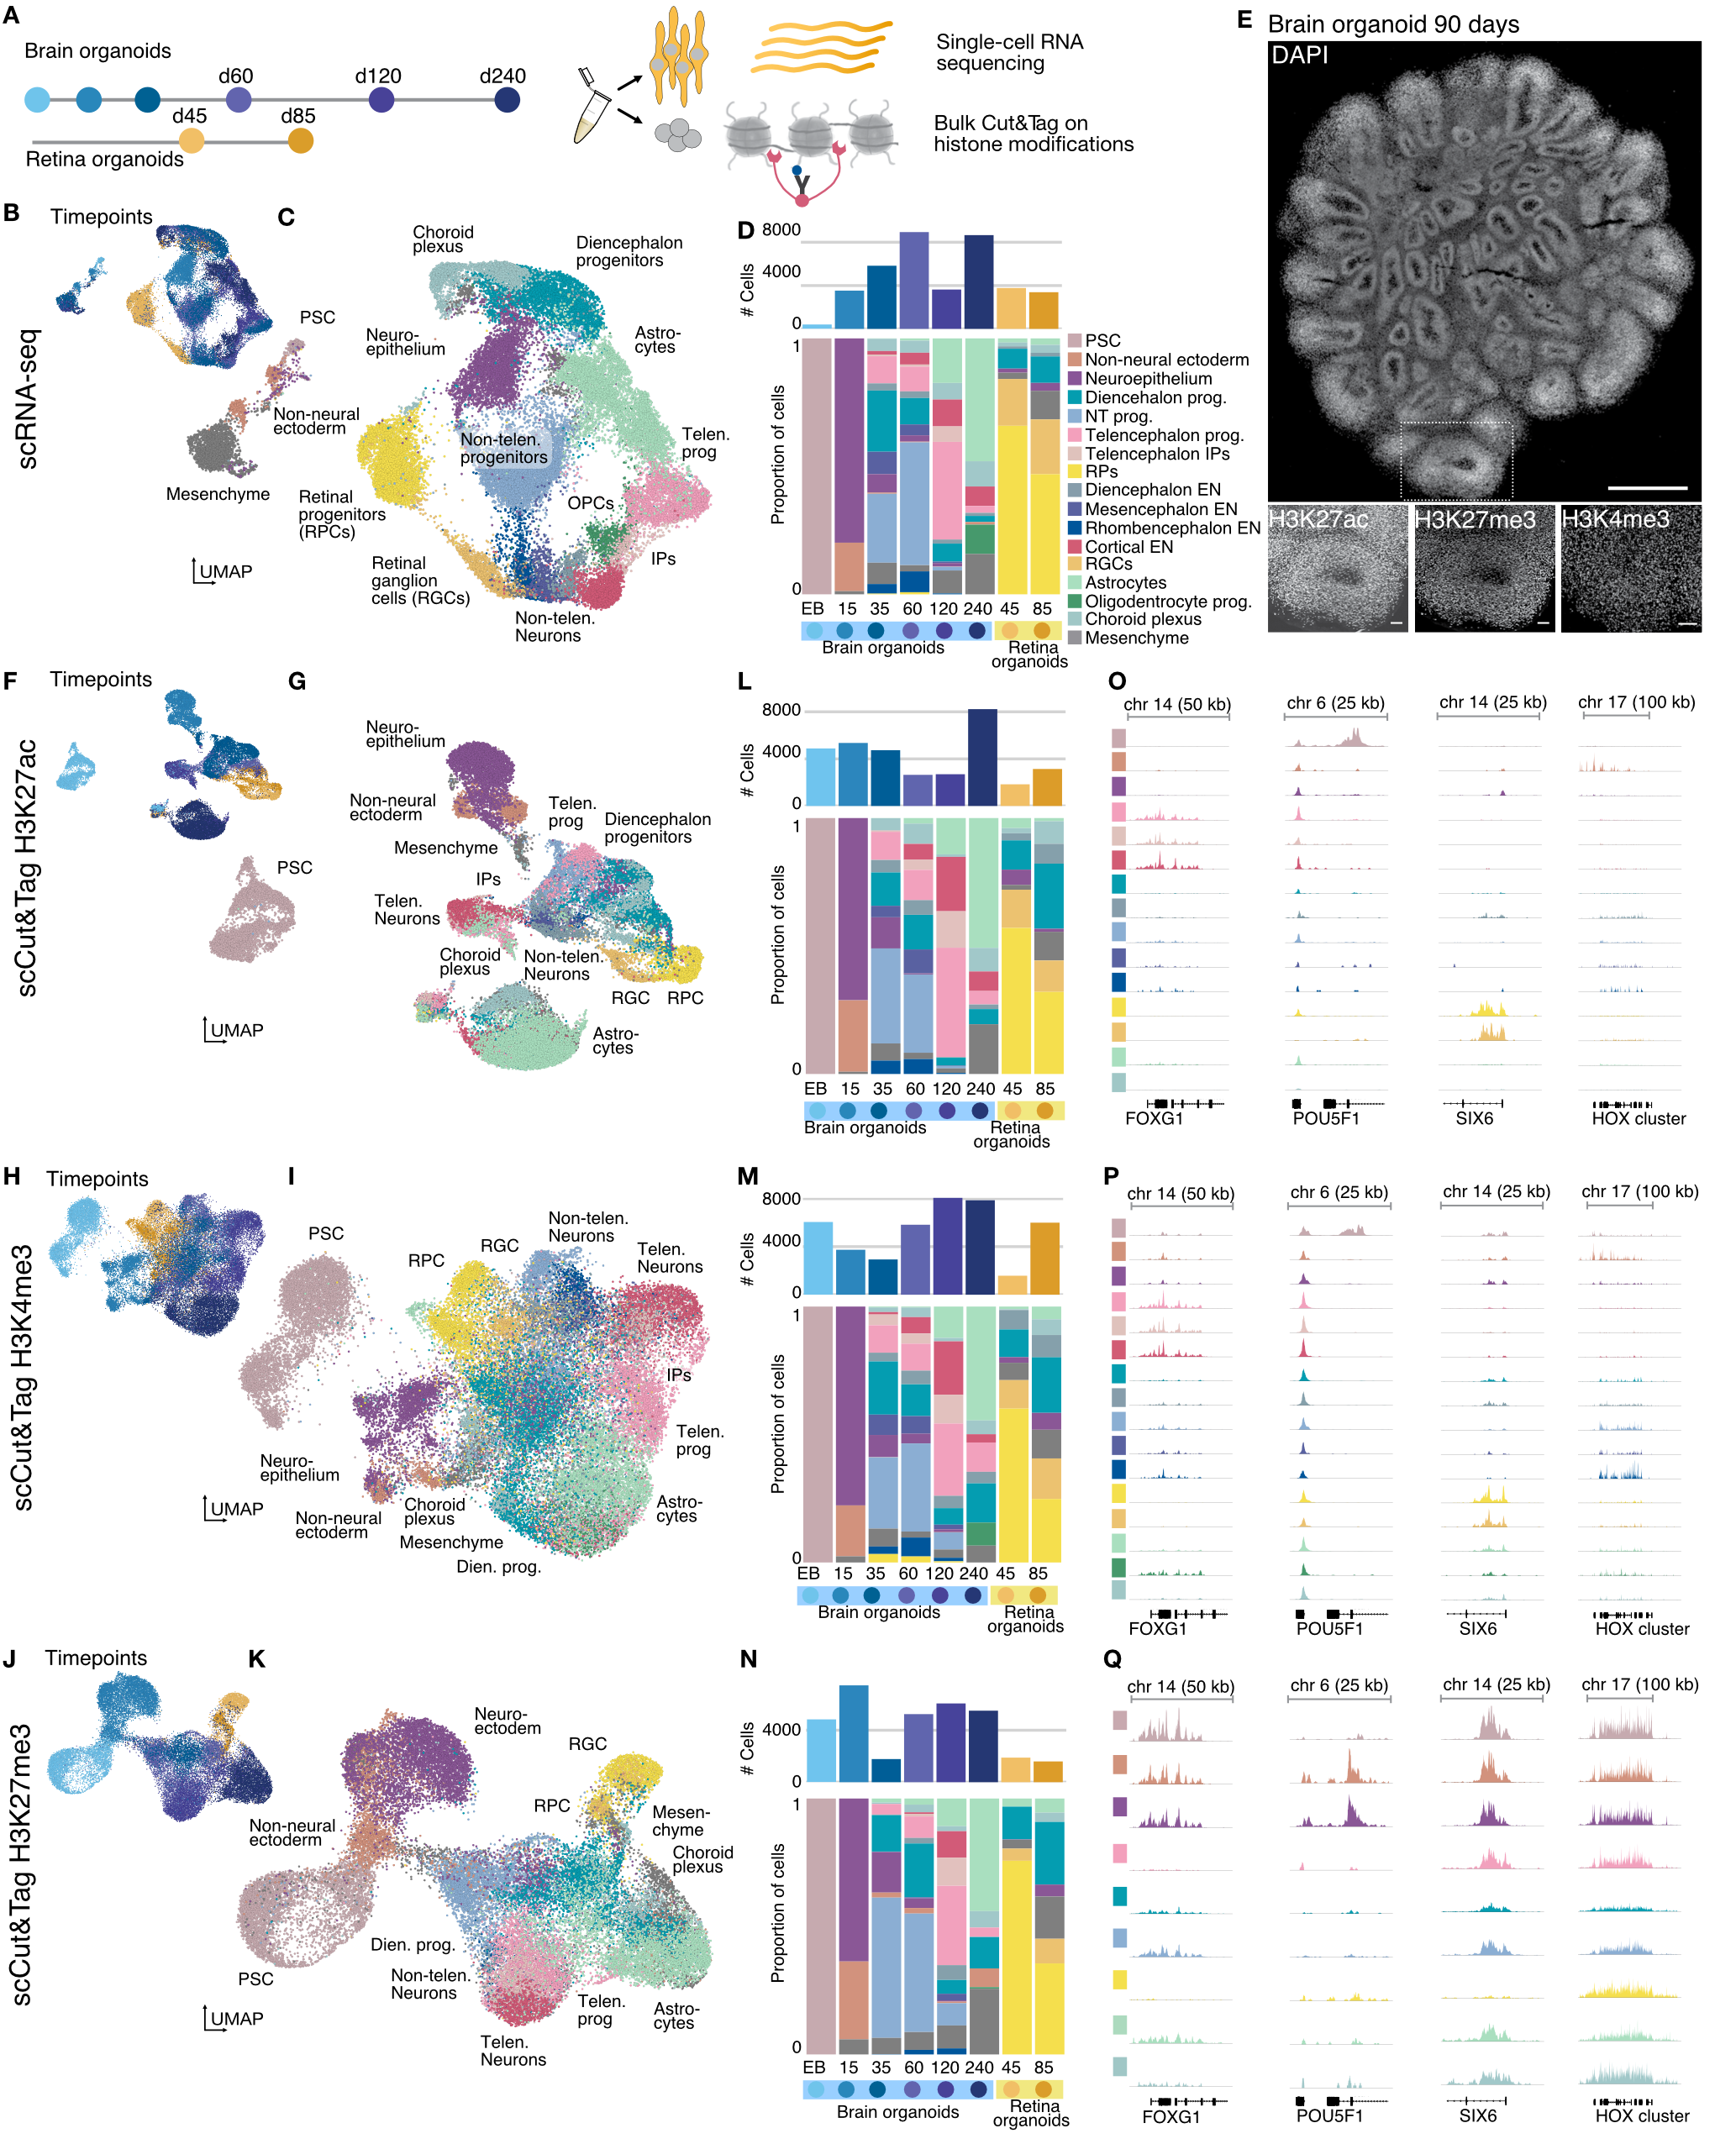
\includegraphics[width=\textwidth]{figures/cnt/Figure_1}
    \label{fig:cnt1}
\end{figure}

\begin{figure}[t!]
    \caption{\textbf{Single-cell epigenomic atlas of brain organoid development from pluripotency.}
    (A) Experimental outline. scCut\&Tag and scRNA-Seq were performed for different developmental timepoints during cerebral and retina organoid development. (B) UMAP embedding with cells colored based on developmental timepoint. (C) UMAP embedding with cells colored by celltype (IP - intermediate progenitor) (D) Bar-plot absolute cell number per timepoint (upper panel). Stacked bar plot of cell type distribution within each timepoint (lower panel) (EN - excitatory neuron, NT-non-telencephalon). (E) DAPI staining of an organoid at day 90, scale bar 1000 $\mu$m (upper panel). One ventricle of an organoid stained for H3K27ac, H3K27me3, H3K4me3, scale bar 100 $\mu$m (lower panel). (F, H, J) Same as (B) for H3K27ac, H3K4me3, H3K27me3, respectively. (G, I, K) Same as (C) for H3K27ac, H3K4me3, H3K27me3, respectively. (L, M, N) Same as (D) for H3K27ac, H3K4me3, H3K27me3, respectively. (O, P, Q) genome browser snapshots show the enrichment of the respective mark at four different marker genes (FOXG1-cortex, POU5F1-pluripotency, SIX6-retina, HOX-cluster-hindbrain and posterior parts of the body). Each signal track represents an annotated celltype.}
\end{figure}

\topparagraph{Single-cell epigenomic reconstruction of brain organoid development}
To address this question in the context of central nervous system development, we performed Cut\&Tag and mRNA-sequencing in single cells (scCut\&Tag and scRNA-seq) on a timecourse of human multi-region brain organoid development, modeling the cell fate transitions from induced pluripotent cells to terminally differentiated neurons. To cover all major lineages and cell types of the developing central nerveous system, we recorded three histone modifications and RNA expression at six developmental time points in brain organoids and two timepoints in retina organoids (Figure 5.1A and Figure S5.1A and B). During organoid development, cells transition from early pluripotent stages (embryoid body; day 5) to a stratified epithelium (neuroepithelium; day 15). From there, progenitors diversify and branch out to develop regional identities (telencephalon, diencephalon, non-telencephalon; day 35 and 60) (Figure 5.1B and C). Brain region-sepecific neurons start to develop from day 35 onward and later increase in abundance (Figure 5.1B, C and D). After day 120, astrocytes and oligodendrocyte precursor cells (OPCs) start to appear in the organoid, coinciding with the gliogenic switch during the second trimester of human embryonic development (Figure 5.1B, C and D) (\cite{rowitch_developmental_2010}). 

Having characterized the cell type and brain regional diversity of the developing organoids we asked how epigenetic changes on chromatin would contribute to fate decisions within the organoids. We first investigated the global distribution of H3K27ac, H3K27me3 and H3K4me3 by immunofluorescence at 90 days of organoid development. We found no major differences during the differentiation from the progenitor (localized at the center of the ventricles) to the neuron stage (localized on the outside of the ventricle) (Figure 5.1E). We then recorded the genome-wide distribution of H3K27ac, H3K27me3 and H3K4me3 by scCut\&Tag from cell suspensions matching scRNA-seq. We obtained high quality data from all experiments as reflected by the nucleosome pattern and the high average number of fragments (H3K4m3 - 2857, H3K27ac - 1723, H3K27me3 - 784) recovered from each cell (Figure S5.1C and D). Dimensionality reduction and embedding with UMAP (\cite{mcinnes_umap_2018}) revealed trajectories from early pluripotent cells over neuroectoderm to more differentiated cell states and brain region identities for each modality (Figure 5.1F-K).

To annotate cell types we first performed high-resolution Louvain clustering (\cite{blondel_fast_2008}) for each modality separately (RNA, H3K27ac, H3K27me3 and H3K4me3). Within high-resolution clusters we obtained on average 104k, 236k and 417k fragments (H3K27me3, H3K27ac and H3K4me3, respectively) and therefore increased the robustness of our analysis. We then annotated the high-resolution clusters of the scRNA-seq data using reference datasets (\cite{kanton_organoid_2019,fleck_inferring_2021}) and marker gene expression. Next, we matched scRNA-seq clusters with corresponding clusters from epigenomic modalities using minimum-cost, maximum-flow (MCMF) bipartite matching (\cite{stark_scim_2020}) based on correlation in case of activating histone marks (H3K27ac and H3K4me3) and anti-correlation in case of repressive mark H3K27me3 (Figure S5.2A and B). Based on these cluster-to-cluster matches we transferred annotated cell state labels from scRNA-seq to other modalities. We found that after label transfer, cell type and state distribution was similar between all modalities, supporting the accuracy of the integration (Figure 5.1L-M). In addition, we detected high enrichment of activating marks at known regulators of cell identity (e.g. FOXG1 in the telencephalic trajectory, POU5F1 in pluripotent stem cells, SIX6 in the retinal trajectory) (Figure 5.1O and P) and found the repressive mark H3K27me3 in cell states where the respective genes are not expressed (Figure 5.1Q). We were able to detect the same pattern of activating and repressive marks on genes marking brain region identities (SIX6, POU5F1, FOXG1, LHX5, NEUROD2, HOXB2) in single cells, which validates our annotation and label transfer (Figure S5.2C). Taken together, we here provide a comprehensive epigenomic atlas of cell type establishment and brain region diversification in organoids.

\begin{figure}[b!]
    \centering
	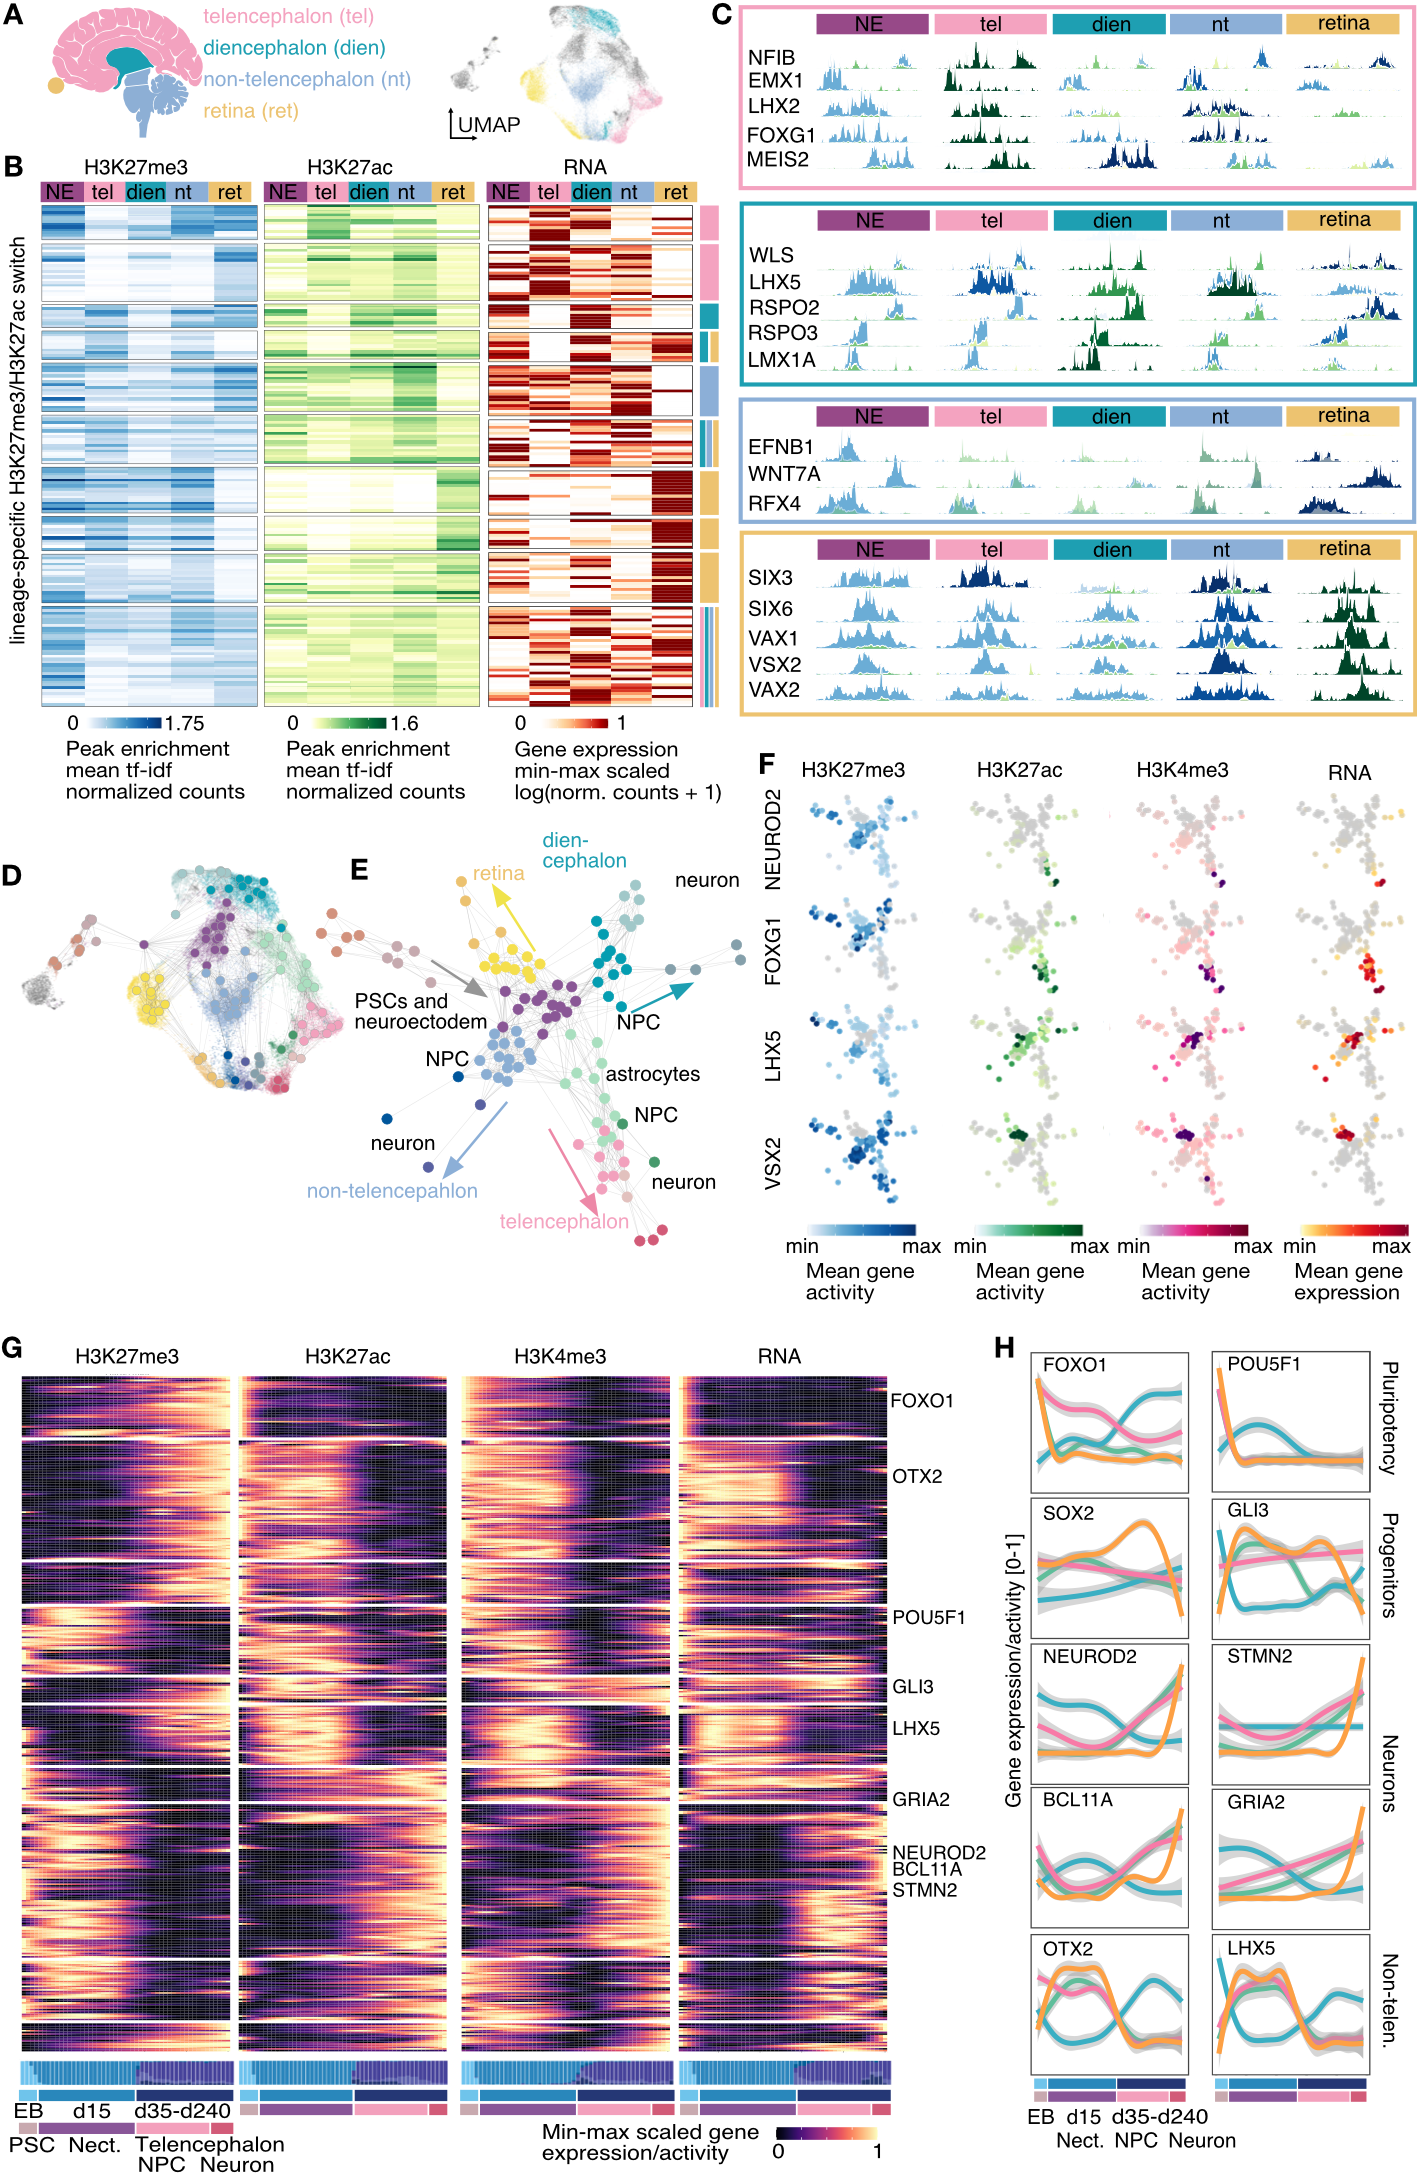
\includegraphics[width=0.9\textwidth]{figures/cnt/Figure_2}
    \label{fig:cnt2}
\end{figure}

\begin{figure}[t!]
    \caption{\textbf{Epigenomic switches and pseudotemporal dynamics during brain region diversification.}
    (A) Schematic of the human brain (left) and UMAP embedding (right) labelled with brain region identities. (B) Heatmap showing peak enrichment of lineage-specific peaks showing switching between H3K27me3 and H3K27ac marks. Expression of the closest gene is shown on the right. (C) Genomic tracks showing switching peaks close to lineage-specific genes. (D) UMAP representation and (E) graph layout of high-resolution clusters labelled by cell type. (F) Graph layout colored by expression and gene activities of all three chromatin marks for NEUROD2, FOXG1 (telencephalon), LHX5 (Non-telencephalon) and VSX2 (retina). (G) Heatmap showing expression and gene activity scores over the telencephalic neuron differentiation trajectory from pluripotency. Pseudotime was binned and genes were K-means clustered based on average expression/activity of all marks and RNA in all bins. (H) Line plots showing smoothed pseudotemporal expression and activities of selected examples from multiple K-means clusters.}
\end{figure}

\topparagraph{Epigenomic switches during regional diversification}
Regulatory elements can switch between a repressed state characterized by H3K27me3 enrichment and an active state marked by H3K27ac (\cite{allis_molecular_2016}). We observed that this is the case for elements in close proximity to many brain region-specific genes, i.e. genes repressed in early developmental stages and active in neurons of a given brain region. To characterize these region-specific switches more systematically, we first grouped all progenitors and neurons in our dataset based on regional identities (Figure 5.2A; telencephalon, non-telencephalon, diencephalon, retina). Next, we assessed regional specificity of peaks by performing differential enrichment analysis. We performed GREAT enrichment analysis (\cite{mclean_great_2010}) on region-specific peaks and found that activating marks H3K27ac and H3K4me3 were enriched in proximity to genes with important regulatory function for the respective region (Figure S5.3). Conversely, region-specific H3K27me3 (repressive) peaks were enriched at diverse genes with little or unspecific functional enrichment. To locate peaks exhibiting a switching behavior upon regional diversification, we intersected region enriched H3K27ac peaks with H3K27me3 peaks showing regional depletion. This revealed a set of peaks that are predominantly repressed during the neuroepithelial stage and switch into an active state in individual regional trajectories (Figure 5.2B). This epigenetic activation was accompanied by region-specific expression of nearby genes (Figure 5.2B), many of which were important regulators of regional identity, such as FOXG1 (telencephalon), RSPO2/3 (diencephalon), WNT7A (non-forebrain) and VSX2 (retina)(Figure 5.2C). Altogether, our analysis indicates that chromatin modifications can induce and stabilize regional diversification events by activating the expression of cell fate regulators.


\topparagraph{Epigenetic activation precedes gene expression during neurogenesis}
We next examined how these chromatin switches change dynamically along the differentiation trajectory from pluripotent stem cells to regionalized neurons. To better visualize the branching of neuroepithelial cells into progenitors and neurons of different brain regions, we used CellRank (\cite{lange_cellrank_2022}) to compute terminal fate probabilities for each regional identity based on RNA expression. We summarized these probabilities for each high-resolution cluster and used them to construct a graph representation of the differentiation events (Figure 5.2D). A force-directed layout of this graph revealed the bifurcation of pluripotent cells into non-neural ectoderm and neuroectoderm, which then diversifies into regional branches (Figure 5.2E). By mapping information from matched high-resolution clusters of chromatin modalities (Figure S5.2B) onto this representation, we could visualize changes in chromatin modifications along the differentiation trajectories (Figure 5.2F). To assess dynamic chromatin changes on the level of genes, we computed activity scores for each gene by summarizing fragment counts for each chromatin modification over the gene body plus an extended promoter region. Visualizing these gene activities on the graph layout made it apparent that many lineage-specific transcription factors were broadly repressed by H3K27me3 outside their expression domain (Figure 5.2F). 
Loss of repression within the respective lineage was accompanied by a gain in activating histone modifications immediately upon regionalization (Figure 5.2F; NEUROD2, FOXG1), which appeared to precede the increase in RNA expression.

To interrogate these developmental changes at higher resolution, we next examined one individual trajectory in isolation. To this end, we extracted cells belonging to the telencephalic neuron trajectory from pluripotency (PSC, neuroectoderm/neuroepithelium, telencephalon progenitor/neuron) and ordered them along a pseudotime axis using RNA velocity in case of RNA (\cite{bergen_generalizing_2020}) and diffusion maps in case of chromatin marks (\cite{haghverdi_diffusion_2016}). In order to obtain an even timepoint distribution over pseudotime for all modalities, we sub-sampled cells before grouping them into 50 equally sized bins (Figure 5.2G). After binning, the distribtion of sampling timepoints was similar between modalities and correlated well with pseudotemporal progression. 

To explore the dynamics of gene activation and repression during differentiation, we clustered genes based on their mean gene activity and expression within pseudotime bins. This revealed three major groups of genes with different switching dynamics. The first group exhibited a major switch between pluripotency and neuroectoderm stages, the second one between neuroectoderm and neural progenitor cell stages and the third one between neural progenitors and neurons (Figure 5.2G). We observed that during development many neuronal genes lose H3K27me3 mediated repression before accumulating H3K27ac and H3K4me3 and ultimately starting RNA expression (Figure 5.2G and H; NEUROD6, BCL11A, STMN2). These results support a model in which chromatin can be primed with activating histone modifications directing the expression of target genes in the future. At the same time, we captured the silencing of non-neuronal genes when cells exit from pluripotency and transition to neuroepithelium. These genes become down-regulated and lose active histone modifications while gaining H3K27me3 at the neuroepithelium stage. At more differentiated stages, these genes can remain silenced in absence of H3K27me3 (Figure 5.2G and H; POU5F1).

\begin{figure}[b!]
    \centering
	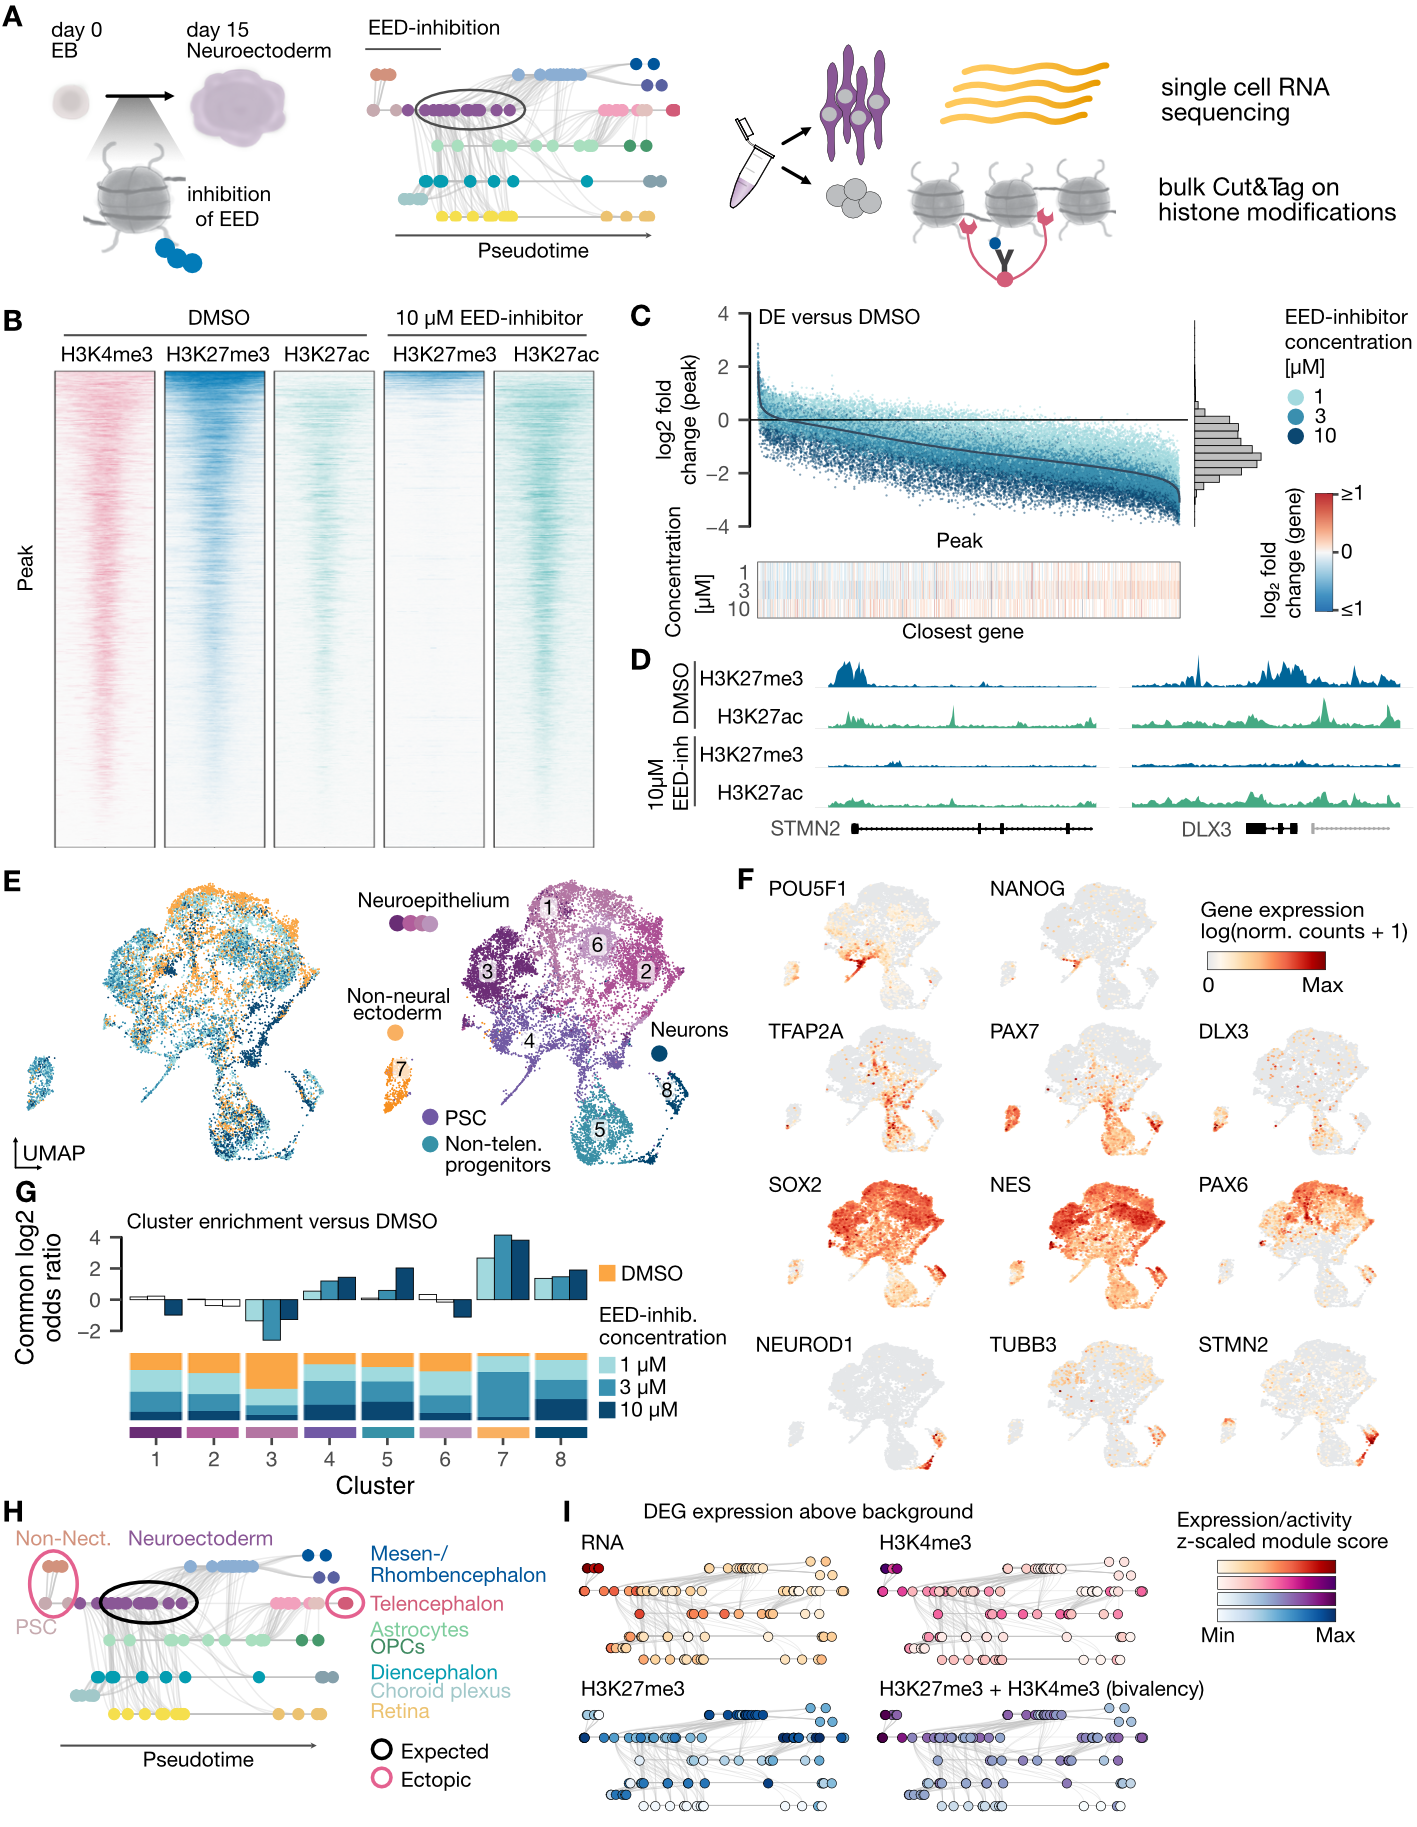
\includegraphics[width=0.9\textwidth]{figures/cnt/Figure_3}
    \label{fig:cnt2}
\end{figure}

\begin{figure}[t!]
    \caption{\textbf{Aberrant fate acquisition upon perturbation of EED.}
    (A) Schematic of the experiment. Organoids were treated with EED inhibitor from day 0 to day 15. During the neuroepithelium stage (day 15-18) organoids were profiled with scRNA-seq and bulk Cut\&Tag. (B) Heatmaps showing peak intensities from the bulk Cut\&Tag experiment for EED-inhibitor (10$\mu$M) and DMSO-treated organoids. Regions are ordered by H3K27me3 intensity. (C) Scatter plot showing log$_2$ fold change of peak intensities of organoids treated with different EED-inhibitor concentrations versus the DMSO control and histogram showing distribution of fold changes (top). Heatmap showing the log$_2$ fold change of expression of the closest gene from DE analysis in scRNA-seq data. (D) Genomic tracks showing bulk Cut\&Tag profiles for H3K27me3 and H3K27ac at genomic regions around STMN2 and DLX3. (E) UMAP embedding of the scRNA-seq data colored by treatment (left) and annotated louvain clusters (right). (F) UMAP embedding colored by expression of genes marking annotated populations. (G) Bar plot showing cluster enrichment of treated cells versus DMSO control (top) and distribution of treatments in clusters (bottom). Common odds ratio (height) and p-value (alpha) were obtained from a CMH-test stratified by sampling timepoint. (H) Tree representation of high-resolution clusters in the developmental timecourse, with the x-axis representing mean pseudotime. Cell populations commonly expected at day 15 (expected, black) and treatment-enriched populations (ectopic, red) are highlighted. (I) Tree representation colored by module scores (deviation above background) of DE gene expression and activity in the developmental timecourse.} 
\end{figure}


\topparagraph{Perturbation of histone modifiers causes aberrant fate acquisition}
The dynamic changes of histone modifications during regionalization and neurogenesis indicate that these epigenetic mechanisms play an important role in cell fate determination. To further investigate the role of histone modifications in shaping brain organoid development and cell differentiation, we chemically inhibited the writer complex of H3K27me3 (EED/PRC2) with A395 (\cite{he_eed_2017}) during the exit from pluripotency until the formation of the neuroepithelium (day 0-15). At the neuroepithelial stage (day 15-18) we profiled the organoids using scRNAseq and bulk Cut\&Tag (Figure 5.3A). Bulk Cut\&Tag measurements of histone modifications in EED-inhibitor and DMSO treated organoids showed an almost complete depletion of H3K27me3 marks upon treatment and an enrichment of H3K27ac marks at the same sites (Figure 5.3B). We quantified this depletion by computing the log$_2$ fold change of normalized H3K27me3 peak intensities versus DMSO control and found that repressive peaks were globally depleted in a concentration-dependent manner (Figure 5.3C). Next, we used the scRNA-seq data to quantify changes in gene expression upon treatment and extract a set of differentially expressed genes (DEGs). We observed a general up-regulation of gene expression, with genes in proximity to depleted peaks being more strongly affected. In the highest concentration of EED-inhibitor treatment, nearly all genes next to H3K27me3 peaks were significantly up-regulated (Figure 5.3B). As examples for this, we highlight the genes STMN2 and DLX3, around which repressive peaks are strongly depleted, resulting in an up-regulation of mRNA expression (Figure 5.3D).

We were curious how such drastic changes in gene expression would manifest on the level of cell states. To assess this, we integrated the scRNA-seq data between conditions, performed clustering and annotated the resulting populations (Figure 5.3E and F). As expected from this timepoint, we  observed a large neuroepithelial progenitor population (SOX2, NES, PAX6), but also pluripotent cells (POU5F1, NANOG) as well as populations of non-neural ectoderm (PAX7, DLX3) and neurons (STMN2, NEUROD1). Interestingly, despite the strong gene expression changes observed globally, both treated and control cells were present in all of these populations. However, differential abundance analysis revealed significant enrichment of treated cells in a number of clusters (Figure 5.3G). Most strongly and consistently affected were three ectopic clusters outside the main neuroepithelial population: non-neural ectoderm (cluster 7), pluripotent cells (cluster 4) and neurons (cluster 8). This indicates that treatment causes cells to increasingly adopt ectopic and off-target cell states (Figure 5.3H). To further investigate the relationship between dysregulated genes and cell state specification, we analyzed the expression and chromatin state of DEGs in the developmental atlas (Figure 5.3I). We found that during normal development, DEGs were predominantly repressed in the neuroepithelium and expressed in other populations, including pluripotent stem cells and non-neural ectodermal cells. Of note, DEGs also showed high bivalency (marked by both H3K4me3 and H3K27me3) in treatment-enriched cells states. Taken together, this analysis suggests that H3K27me3-mediated repression is required to stabilize neuroectoderm and neuroepithelium induction from pluripotency. Disruptions of H3K27me3 consequently leads to up-regulation of otherwise repressed or bivalent genes, causing cells to increasingly acquire aberrant and ectopic fates. 


\subsection{Discussion}
During early human brain development, gene expression has to be tightly coordinated to enable controlled differentiation into a multitude of defined cell types. Despite incredible progress in measurement technologies, it has so far remained challenging to interrogate the epigenetic mechanisms that shape these processes on a global scale and with single-cell resolution. 

Here we have addressed this challenge by measuring histone modifications at single-cell resolution in brain organoids, which model early human brain regionalization and cell type establishment \textit{in vitro}. Over a developmental organoid time course, we integrated scCut\&Tag profiles marking repressed and active chromatin states with RNA-expression data. Broadly, we found that chromatin modification profiles were highly specific for a given cell population. We identified region-specific regulatory chromatin regions and found that they controlled important regulators of cell fate. Such regulators were also often marked by epigenetic switches, which shift from repressive to active chromatin states at fate bifurcation events to prime gene expression. Generally, these observations indicate that chromatin modifiers play crucial roles in regional diversification events and stabilize cell fate commitment. This was further supported by perturbation of EED, which caused a global depletion of H3K27me3, an up-regulation of otherwise repressed genes and a strong tendency of cells to adopt off-target cell states. Inerestingly, a large fraction of cells still established neuroectoderm and neuroepithelium, even in the near complete absence of H3K27me3. This suggests that this is a default fate that cells assume in the absence of further inductive signals (\cite{argelaguet_multi-omics_2019,munoz-sanjuan_neural_2002}).  

Altogether, these results suggest that dynamic chromatin modifications are required to ensure robust cell fate acquisition and brain regionalization. Moreover, our developmental atlas of histone marks is the first of its kind and will serve as a reference to better understand the epigenomic landscape of human brain development.




\subsection{Methods}

\paragraph{Cell and organoid culture}
For culturing cells were grown on matrigel (Corning, \#354277) coated 6-well dishes in mTeSR Plus (StemCell Technologies, \#100-0276) supplemented with penicillin/streptomycin (P/S, 1:200, Gibco, \#15140122). To propagate the cells, they were dissociated with TryplE (Gibco, \#398 12605010) or EDTA in DPBS (final concentration 0.5mM) (Gibco, \#12605010) and kept on Rho-associated protein kinase (ROCK) inhibitor Y-27632 (final concentration 5 $\mu$M, StemCell Technologies, \#72302) for one day. Cells were stored in liquid nitrogen in mFreSR (StemCell Technologies, \#05855) and tested for mycoplasma (Venor GeM Classic, Minerva Biolabs) after each thawing cycle. 

To generate cerebral organoids, cells were grown to a confluency of around 50\% and dissociated with TryplE. 2000-3000 cells were aggregated in 96-well ultra low attachment plates (Corning, \#CLS7007) to form embryoid bodies (EBs). We followed an unguided protocol to obtain cerebral organoids5, with few modification. EBs were aggregated and cultured in mTeSR Plus and neural induction medium was added when the EBs had reached around 400-500 $\mu$m. Retinoic acid containing neural differentiation medium was only added from day 40 onward. Cerebral organoids were grown shaking in 6 cm dishes for up to 8 month.

To generate retinal organoids, we applied a protocol that allows the simultaneous aggregation of hundreds of embryoid bodies in agarose molds4. These are then transferred (1 week) to and later scraped off from 6-well plates (4 weeks), before they are transferred into differentiation medium.  
The use of human ESCs for the generation of cerebral organoids was approved by the ethics committee of northwest and central Switzerland (2019-01016) and the Swiss federal office of public health.

\paragraph{Drug treatment}
We used a pharmacological approach to inhibit chromatin modifiers in cerebral organoids. Specifically the H3K27-acetylase CBP/P3006 (A485, MedChemExpress, \#HY-107455) and the H3K27me3-reader EED7 (A395, MedChemExpress \#HY-101512, prevents allosteric activation of the PRC2 complex) were targeted. For A395 concentrations between 1-10 $\mu$M were tested and H3K27me3 was depleted in bulk experiments at 1 $\mu$M as shown by western blot. For A485 two concentrations (1 $\mu$M and 3 $\mu$M) were tested and H3K27ac, was depleted at 1 $\mu$M. 

CBP/P300 and EED were inhibited from day 0-15, by adding the inhibitor when seeding the EBs. This time window coincides with the formation of the neural epithelium. Following the medium was changed every 3 days adding a fresh dose of inhibitors. 
In a second experiment, CBP/P300 and EED were inhibited with 1 and 3 $\mu$M of the respective inhibitor from day 12-21, when brain regional markers start to be expressed in the organoid. 

To rule out cell line specific effects we treated two different cell lines (HOIK1 and WIBJ2) for the early timepoint and three (HOIK1, WIBJ2, WTC for 3 $\mu$M A395 and 1 $\mu$M A485) to five different cell lines (409b2- iCRISPR, B7, WTC, HOIK1 and WIBJ2 for DMSO, 1 $\mu$M A395 and 3 $\mu$M A485) for the late timepoint. We used single nucleotide polymorphisms (SNPs) to assign the cells bioinformatically to each cell line.

\paragraph{Preparation of single cell suspensions}
Cerebral organoids were generated in batches. In each batch five different stem cell lines (409b2- iCRISPR, B7, WTC, HOIK1 and WIBJ2) were used and dissociated together. The cell lines were later demultiplexed using single nucleotide polymorphisms (SNPs). For retinal organoids only B7 was used. We sampled all important developmental transitions from the pluripotent EB (day 5) and neuroepithelium (day 15) to neuronal differentiation in cerebral (day 35, 60, 120, 240) and  in retinal organoids (day 45 and 85). Organoids were cut into small pieces using a scalpel and thoroughly washed with HBSS buffer without Ca2+/Mg2+ (StemCell Technologies, \#37250) to remove debris. 

To obtain single cell suspension a papain-based neural dissociation kit (Miltenyi Biotec, 130-092-628) was used. In brief, 1900 $\mu$l of pre-warmed buffer X with 50 $\mu$l of Enzyme P were added to the organoids and incubated for 15 min at 37 °C. Subsequently, a mix of 20 $\mu$l buffer Y and 10 $\mu$l of DNase was added to each sample before tituration (10 times with a p1000 wide bore tip, 10 times with a p1000 wide bore tip). The samples were then incubated twice for another 10 min and titurated with a p1000 and p200 in between
 
At the end, the reaction was stopped with HBSS buffer without Ca2+/Mg2+ and the cells were passed through a 30 $\mu$m strainer. After an additional wash the cells were then stored in CryoStor CS10 (StemCell Technologies, Catalog \# 07930) or processed right away for further experiments. For all scCut\&Tag experiments, cells were kept from the same cell suspension to perform scRNA sequencing. Cell suspension usually exhibited viabilities between 80-95\%

\paragraph{Cloning and purification of Tn5}
Plasmids \#123461 (pA/G-MNase) and \#124601 (3XFlag-pA-Tn5-Fl) were ordered from Addgene. ProteinA and ProteinG were amplified using the primer pairs (FZ461\_ProtA\_rev,  
FZ462\_HindIII\_ProtA\_fw and FZ459\_EcoRI\_ProtG\_rev, FZ460\_ProtG\_fw) and fused by PCR (all primer sequences are in Table X, below). The ProteinA in the original vector (3XFlag-pA-Tn5-Fl)  was then replaced with the fusion product through EcoRI and HindIII restriction digest. 

The final plasmid was transformed into chemically competent Rosetta cells to express the protein. The bacteria were grown to OD600~0.4-0.6, expression was induced with 0.25 mM IPTG and the protein was expressed at 18 °C overnight. Cells were harvested and stored at -80 °C until further processing. The purification was performed on Chitin resin (New England Biolabs, \#S6651S) as described8, with small modifications. The cells were lysed using the Diagenode Bioraptor Plus at the high setting for 15 cycles 30 sec on/30 sec off.
After dialysis and concentration using Amicon Ultra-4 Centrifugal filters (Millipore, \#UFC803024) the protein was diluted to 50\% glycerol final and loaded with adapters before use: \\
FZ459\_EcoRI\_ProtG\_rev	gaattctttatcgtcatctacggctggcgtcaactcagacgcg \\
FZ460\_ProtG\_fw	aaaaagctaaacgatgctcaagcaccaaaaacaacttataaattagtcatcaacggg \\
FZ461\_ProtA\_rev	aatttataagttgtttttggtgcttgagcatcgtttagctttttagcttctgc \\
FZ462\_HindIII\_ProtA\_fw	ccaagcttaaaagatgacccaagccaaagtgctaacc \\
FZ444\_Tn5MErev	[phos]CTGTCTCTTATACACATCT \\
FZ445\_Tn5ME-A	TCGTCGGCAGCGTCAGATGTGTATAAGAGACAG \\
FZ445\_Tn5ME-B	GTCTCGTGGGCTCGGAGATGTGTATAAGAGACAG \\

\paragraph{Single cell Cut\&Tag}
Starting from 1.5-3 Mio cells, nuclei were isolated following the 10x Genomics CG000365 Demonstrated Protocol. The 0.1x buffer was used for all experiments, adjusting the final concentration of Digitonin to 0.01\% (Thermofisher, BN2006). In general we followed the bulk Cut\&Tag protocol with a few adjustments. 
After lysis the nuclei were directly transferred into scCut\&Tag wash buffer (20 mM HEPES [pH 7.5] (Jena Bioscience, \#CSS-511), 150 mM NaCl (Sigma Aldrich, \#S6546), 0.5 mM Spermidine (Sigma Aldrich, \#S0266), 1\% BSA (Miltenyi, \# 130-091-376), 1 mM DTT (Sigma Aldrich, \#10197777001), 5 mM sodium butyrate (Sigma Aldrich, \#303410), Roche Protease Inhibitor (Sigma Aldrich, \#11873580001)) and washed once for 3 min at 300 xg. The buffer was then supplemented with 2 mM of EDTA before the antibodies were added (see Table X for further details). The samples were then incubated on a rocking platform at 4 °C overnight. 

The next morning the cells were washed once and the secondary antibody was added to the suspension for 1 hr at 20 °C on a rocking platform or Eppendorf Thermomixer. The cells were then washed twice and transferred into scCut\&Tag med buffer (20 mM HEPES [pH 7.5] (Jena Bioscience, \#CSS-511), 300 mM NaCl (Sigma Aldrich, \#S6546), 0.5 mM Spermidine (Sigma Aldrich, \#S0266), 1\% BSA (Miltenyi, \# 130-091-376), 1 mM DTT (Sigma Aldrich, \#10197777001), 5 mM sodium butyrate (Sigma Aldrich, \#303410), Roche Protease Inhibitor (Sigma Aldrich, \#11873580001)) including 2 $\mu$g of homemade Tn5. The cells were incubated for 1 hr at 20 °C and then washed again twice with scCut\&Tag med buffer. To induce the cutting of the Tn5, 1 mM final MgCl2 (Sigma Aldrich, \#M1028) was added and the sample was incubated for 1 hr at 37 °C. After the incubation, the reaction was stopped with 15 mM EDTA final and the sample was filled to 600 $\mu$l with diluted nuclei buffer of the 10x Genomics scATAC kit v1.1 supplemented with 2\% BSA. The nuclei were filtered through a 40 $\mu$m Flowmi filter (Sigma Aldrich, \#BAH136800040) and washed with diluted nuclei buffer supplemented with 2\% BSA.

The final nuclei suspension quality controlled and counted with a Trypan Blue assay on the automated cell counter Countess (ThermoFisher). Finally 15-20k nuclei were loaded per experiment, in cases were fewer nuclei were recovered all were loaded. To run the Chromium Chip, 5 $\mu$l of cell suspension were mixed with 3 $\mu$l of PBS and 7 $\mu$l of ATAC buffer from the kit. 

Libraries were prepared following the manufacturer's instructions, except that 2 PCR cycles were added to the barcoding PCR and after 10 cycles of indexing PCR 5 $\mu$l of the library were used to determine the final number of cycles in a Roche LightCycler9. Usually sCut\&Tag libraries required 12-16 PCR cycles during the indexing. After SPRI select clean-up (Beckman Coulter, \#B23318) the libraries were quality controlled and sequenced following the 10x Genomics scATAC v1.1 sequencing recommendations. Usually 50-100 Mio reads per library were enough to cover the complexity. 

\paragraph{Bulk Cut\&Tag}
Starting with 0.1-1 Mio cells after dissociation, cells were transferred into Cut\&Tag wash buffer (20 mM HEPES [pH 7.5] (Jena Bioscience, \#CSS-511), 150 mM NaCl (Sigma Aldrich, \#S6546), 0.5 mM Spermidine (Sigma Aldrich, \#S0266), 5 mM sodium butyrate (Sigma Aldrich, \#303410), Roche Protease Inhibitor (Sigma Aldrich, \#11873580001)). Following 15 $\mu$l of BioMag ConcavalinA beads (Polysciences, \#86057-3) in binding buffer (20 mM HEPES (pH 7.5), 10 mM KCl, 1 mM CaCl2, 1 mM MnCl2) were added to the sample and incubated on the wheel for 15 min at RT. Subsequently the cells were collected on a magnet and lysed through the addition of Cut\&Tag wash buffer supplemented with 0.01\% Digitonin. Lysis was monitored under a microscope with Trypan Blue staining. After lysis was complete the nuclei were washed again with Cut\&Tag wash buffer. If possible all samples were split and H3 or another chromatin mark Cut\&Tag was performed on the same starting material, to be used as normalizer. The antibody was added together with 2 mM EDTA final and the sample was incubated on a rocking platform at 4 °C overnight.  
The samples were washed once with Cut\&Tag wash buffer and the secondary antibody was added to the reaction and incubated for 1 hr at 20 °C on a rocking platform. After two additional washes the Tn5 was added (1:100) in Cut\&Tag med buffer (20 mM HEPES [pH 7.5] (Jena Bioscience, \#CSS-511), 300 mM NaCl (Sigma Aldrich, \#S6546), 0.5 mM Spermidine (Sigma Aldrich, \#S0266), 5 mM sodium butyrate (Sigma Aldrich, \#303410), Roche Protease Inhibitor (Sigma Aldrich, \#11873580001)). Tn5 was allowed to bind for 1 hr at 20 °C on a rocking platform. After two additional washes the cutting was induced through addition of 1 mM MgCl2 in Cut\&Tag med buffer. After 1 hr at 37 °C the reaction was stopped by adding a final of 20 mM EDTA, 0.5\% SDS and 10 mg Proteinase K. The reaction was then incubated at 55 °C for 30 min and finally inactivated at 70 °C for 20 min.
 The DNA fragments were purified using the ChIP DNA Clean \& Concentrator kit (Zymo Research, \#D5205) for the elution from the columns 2 pg of Tn5-digested and purified lambda DNA (New England Biolabs, \# N3011S) were added to be used as spike-in normalizer for later analysis, when needed.

Purified fragments were indexed for 15 cycles (1 x 5 min at 58 °C, 1 x 5 min at 72 °C, 1 x	30 s at 98 °C, 14x 10 s at 98 °C, 30 s at 63 °C, 1 x 1 min at 72 °C, $\infty$ at 4 °C) using NEBNext HighFidelty 2x PCR Master Mix (New England Biolabs, M0541S) and Illumina i5 and i7 indeces9. The libraries were then purified using AmPure beads (Beckman Coulter, \#A63881), measured and quality controlled with Qubit DNA HS Assay (ThermoScientific, \#Q32854) and on the Tapestation (Agilent, \#5067-4626) and then sequenced (PE, 2x50 bp).

\paragraph{Hashing and single cell RNA-Seq}
Cells were either processed right after dissociation or recovered after cryostoring.  To recover the cells after cryostoring, the cryovials were incubated in a waterbath at 37 °C until only a small ice-piece was left inside the tube. The cells were then transferred into prewarmed DMEM/F-12 (Gibco, \#31330038) supplemented with 10\% FBS final (Merck, \#ES-009-B). After washing twice with DPBS (Gibco, \# 14190144) supplemented with 0.5\% BSA the cells were filtered with a 40 $\mu$m Flowmi filter and counted using the Trypan Blue assay on the automated cell counter Countess (ThermoFisher). Usually cell viability was around 80-95\%. At this point cells were further diluted to be processed in the 10x Genomics single cell RNA expression v3.1 assay following strictly the manufacturer's guidelines.

To generate single cell RNA expression libraries of the drug treatment we turned to cell hashing10 for better comparability of the samples. For hashing 100-300 k cells were resuspended in 50-100 $\mu$l of DPBS+0.5\% BSA. Following 5 $\mu$l of the Human TruStain FcX (Fc Receptor Blocking Solution, BioLegend, \#422302) were added to the sample and incubated for 10 min on ice.  Next, the 2 $\mu$l TotalSeq Cell hashing antibodies (BioLegend) were added to the cells and incubated for 30 min on ice with gentle agitation every 10 min. After incubation cells were washed twice with DBPS+0.5\% BSA. Depending on the starting amount the cells were resuspended in 20-40 $\mu$l DPBS+0.5\% BSA and counted. Following the cell suspensions were mixed and processed in the 10x Genomics single cell RNA expression v3.1 assay following strictly the manufacturer's guidelines with slight adjustments. A maximum of 20 k cells was targeted per experiment and HTO additive primer was added to the cDNA synthesis following the TotalSeq technical protocol (https://www.biolegend.com/en-us/protocols/totalseq-a-antibodies-and-cell-hashing-with-10x-single-cell-3-reagent-kit-v3-3-1-protocol). The generate gene expression and hashing libraries we followed the protocol CG000206 Chromium Next GEM SingleCell v3.1 Cell Surface Protein and sequenced according to the manufacturer's guidelines.

\paragraph{Western Blot}
Depending on the timepoint 1-3 organoids were directly collected into 50 $\mu$l Laemmli sample buffer and homogenized with an electric grinder (Fisherbrand 12-141-368). DNA was sheared by sonication in the Diagenode Bioraptor Plus (high setting for 15 cycles 30 sec on/30 sec off). Samples were subsequently run on SDS- PAGE and transferred to PVDF membrane using Wet-Blot. 2-10 $\mu$l of extract were loaded per lane. The ECL signal was recorded using iBright system (Invitrogen). The signal was compared to antibody stainings of loading controls (H3 and $\beta$-Catenin) and the membranes were quality controlled by Ponceau (Sigma Aldrich, \#P7170-1L) staining. See Table for details on the antibodies.

\paragraph{Immunostaining}
Organoids were fixed overnight in 4\% PFA. The next day, the organoids were washed three times for 5 min with DPBS and then transferred into 30\% sucrose in DPBS until they sank to the bottom of the tube. Following the organoids were transferred into cryomolds (Sakura, \#4565) and embedded in Tissue-Tek O.C.T. (Sakura, \#16-004004) on dry ice. The organoids were then sliced at the Cryostar NX70 (Thermo Scientific) into 20 $\mu$m thick slices at -17 °C. The slices were transferred to glass slides and washed with PBS. After a quick wash, antigen retrieval was performed for 20 min at 70 °C in 1x preheated HistoVT one (Nacalai, \#06380). Slides were washed 3 times for 5 min with PBS+0.2\% Tween and then transferred to blocking and permeabilization (PBS, 0.1\% Triton, 5\% Serum, 0.2\% Tween, 0.5\% BSA) for 1 hr. The antibodies were added in blocking solution overnight at 4 °C (see table for further details). The next day the slides were washed again 3 times for 5 min with PBS+0.2\% Tween and the secondary antibody was added in PBS supplemented with 2\% BSA and 0.2\% Tween for 2 hrs at room temperature. Last the slides were washed again 3 times for 5 min with PBS+0.2\% Tween adding DAPI to the last wash. The slides were then mounted in Prolong Glass Antifade and imaged at the Nikon Ti2 Spinning Disk or at the confocal Zeiss LSM980. 

\paragraph{Preprocessing scRNA-seq data}
To compute transcript count matrices sequencing reads were aligned to the human genome and transcriptome (hg38, provided by 10x Genomics) by running Cell Ranger (version 5.0.0)with default parameters. Count matrices were then preprocessed using the Seurat R package (version 3.2)(\cite{stuart_comprehensive_2019}). Cells were filtered by unique molecular identifier (UMI) counts, number of detected genes, and fraction of mitochondrial genes as follows:

\begin{itemize}
    \item \# UMIs > 2000 
    \item \# UMIs < 1.5 * 10\textsuperscript{5} 
    \item \# detected genes > 1000 
    \item fraction of mitochondrial reads < 0.2
\end{itemize}

Transcript counts were normalized by the total number of counts for that cell, multiplied by a scaling factor of 10,000 and subsequently natural-log transformed (NormalizeData()).

\paragraph{Preprocessing and clustering of scCut\&Tag data}
We aligned the sequencing reads to the human genome and transcriptome (hg38, provided by 10x Genomics) using Cell Ranger ATAC (version 1.2.0) with default parameters to obtain fragment files and peak calls. FThe fragment files and the peak count matrices were further preprocessed using Seurat (version 3.2)\cite{stuart_comprehensive_2019} and Signac (version 1.1)(\cite{stuart_multimodal_2020}). The following quality control metrics were computed using Signac: A transcription start site (TSS) enrichment score (TSSEnrichment()), nucleosome signal (NucleosomeSignal()), the percentage of reads in peaks, and the ratio of reads in genomic blacklist regions. Subsequently, cells with less than 200 (H3K27ac, H3K4me3) or 100 (H3K27me3) fragment counts were filtered out.

We then created a unified set of peaks from the union of peaks from all samples by merging overlapping and adjacent peaks. The unified set of peaks was requantified for each sample using the fragment file (FeatureMatrix()). Peak counts were normalized by term frequency-inverse document frequency (tf-idf) normalization using the Signac functions RunTFIDF(). Latent semantic indexing (LSI) was performed by running SVD (RunSVD()) on the tf-idf-normalized matrix. To visualize the data in 2D, Uniform Manifold Approximation and Projection (UMAP)(\cite{becht_dimensionality_2019}) was performed on LSI components 2-30. We then called high-resolution clusters using Louvain clustering in each group separately with the following resolutions to obtain similar cluster sizes:

\begin{itemize}
    \item EB: 2
    \item mid: 5
    \item late: 10
    \item 8 months: 5
    \item retina: 5
\end{itemize}


\paragraph{Demultiplexing}
We used demuxlet (\cite{kang_multiplexed_2018}) to demultiplex cells pooled from different stem cell lines. For B7 and 409B2-iCRISPR single nucleotide polymorphisms were called using bcftools based on DNA-seq data1,14 or downloaded from the HipSci website (HOIK1, WIBJ2) and the Allen Cell Atlas (WTC). All files were merged using bcftools and sites with the same genotypes in all samples were filtered out. Demuxlet was run with default settings. Cells with ambiguous or doublet assignments were removed from the data. Otherwise, the best singlet assignment was considered the lines' genotype.


\paragraph{Integration and annotation of scRNA-seq data}
First, we grouped the dataset into 5 groups depending on the sample of origin:  

\begin{enumerate}
    \item EB: 4 days old brain organoids in EB stage
    \item mid: 15 days old brain organoids in neuroectoderm stage
    \item late: 1-4 month old brain organoids
    \item 8 months: 8 month old brain organoids
    \item retina: 6 week \& 12 week old retina organoids
\end{enumerate}

Initial integration was based on mid and late groups. We computed the 2000 most variable features using the Seurat function FindVariableFeatures() and computed cell cycle scores using the Seurat function CellCycleScoring(). Subsequently the data was z-scaled, cell cycle scores were regressed out (ScaleData()) and Principal Component Analysis (PCA) was performed using the Seurat function RunPCA() based on variable features. We used the first 10 principal components (PCs) to integrate the different timepoints in the dataset using the Cluster Similarity Spectrum method (CSS)(\cite{he_css_2020}). The missing samples EB, retina and 8 months were then projected into CSS space using the css\_project() function. To obtain a two-dimensional representation of the data we performed Uniform Manifold Approximation and Projection (UMAP)(\cite{becht_dimensionality_2019}) using RunUMAP() with spread=0.8, min.dist=0.2 and otherwise default parameters.

To annotate the data, we first called high-resolution clusters using Louvain clustering in each group separately with the following resolutions to obtain similar cluster sizes:

\begin{itemize}
    \item EB: 1
    \item mid: 2
    \item late: 5
    \item 8 months: 2
    \item retina: 2
\end{itemize}

Clusters were annotated with cell types and regional identities using VoxHunt (\cite{fleck_resolving_2021}), comparison to reference datasets (\cite{kanton_organoid_2019,fleck_inferring_2021}) and marker expression.

\paragraph{Hashing}
Count matrices were generated with CITE-seq-Count (version 1.4.5 running under Python version 3.6.13) and intersected with transcript matrices from Cell Ranger. The hashtag counts were normalized with centered log-ratio (CLR) transformation. Doublets were filtered out using hashtag information. 

\paragraph{Calculation of gene activity scores}
To enable comparison of gene expression with chromatin modifications in the same feature space, we computed gene activity scores for each gene and chromatin modality. For this we used the Signac function GeneActivity() with default parameters. Fragment counts representing gene activities were subsequently log-normalized with a scaling factor of 10,000. 

\paragraph{Matching of scRNA and scCut\&Tag data}
To integrate cell populations between RNA and chromatin modalities, we matched high-resolution clusters based on correlation of gene expression with gene activity scores. For this, we performed minimum-cost maximum-flow (MCMF) bipartite matching between the modalities as described in \cite{stark_scim_2020} \\(https://github.com/ratschlab/scim). The function get\_cost\_knn\_graph() was used with \\knn\_k=10, null\_cost\_percentile=99 and capacity\_method='uniform'. As a distance metric (knn\_metric), we used the correlation distance provided by scipy (\cite{virtanen_scipy_2020}) for activating marks H3K27ac and H3K4me3 and the negative correlation distance for repressive mark H3K27me3. Unmatched clusters from either modality were matched based on maximum (or minimum) correlation. 


\paragraph{RNA velocity and inference of terminal fate probabilities}
To obtain count matrices for the spliced and unspliced transcriptome, we used kallisto (version 0.46.0)(\cite{bray_near-optimal_2016}) by running the command line tool loompy fromfastq  from the python package loompy (version 3.0.6)(https://linnarssonlab.org/loompy/). RNA velocity was subsequently calculated using scVelo (version 0.2.4)(\cite{bergen_generalizing_2020}) and further analyzed using scanpy (version 1.8.2)(\cite{wolf_scanpy_2018}). First, 2000 highly variable features were selected using the function scanpy.pp.highly\_variable\_genes(). Subsequently, moments were computed in CSS space using the function scvelo.pp.moments() with n\_neighbors=20. RNA velocity was calculated using the function scvelo.tl.velocity() with mode='stochastic' and a velocity graph was constructed using scvelo.tl.velocity\_graph() with default parameters. To order cells in the developmental trajectory, a root cell was chosen randomly from cells of the first time point (EB) and velocity pseudotime was computed with scvelo.tl.velocity\_pseudotime().  The obtained velocity pseudotime was further rank-transformed and divided by the total number of cells in the dataset. Based on the velocity pseudotime, we computed fate probabilities into the following manually annotated terminal cell states: Dorsal telencephalon neurons, diencephalon neurons, midbrain neurons, hindbrain neurons, retinal ganglion cells, astrocytes, oligodendrocyte progenitors, non-neural ectoderm and choroid plexus. For this, we used CellRank (version 1.3.0)(\cite{lange_cellrank_2022}). A transition matrix was constructed with a palantir kernel (PalantirKernel()) based on velocity pseudotime. Absorption probabilities for each of the predefined terminal states were computed using the GPCCA estimator.


\paragraph{Graph representation of the scRNA-seq data}
To better visualize the differentiation trajectories, we computed a graph representation based on the computed fate probabilities. First, we used PAGA to compute the connectivites between clusters (scvelo.tl.paga()) and summarized transition scores for each of the clusters. To find branch points at which the transition probabilities into different fates diverge, we then constructed a nearest-neighbor graph between the high-resolution clusters based on their transition scores (k=10). We further pruned the graph to only retain edges going forward in pseudotime, i.e. from a node with a lower velocity pseudotime to a node with a higher velocity pseudotime. Additionally, we removed edges connecting different regional trajectores. The resulting graph is directed with respect to pseudotemporal progression and represents a coarse-grained abstraction of the fate trajectory, connecting groups of cells with both similar transition probabilities to the different trajectories and high connectivities on the transcriptomic manifold. 


\paragraph{Trajectory reconstruction}
To reconstruct the telencephalic trajectory from pluripotency in higher resolution, we first extracted all cells annotated as EB, neuroepithelium, telencephalic progenitors and neurons. We next sought to compute a pseudotime describing the progression along this trajectory for all modalities separately. For all chromatin modalities, we used LSI components 2-10 to compute diffusion maps with the R package destiny (\cite{haghverdi_diffusion_2016}). Ranks along the first diffusion component were used as a pseudotemoral ordering. For RNA, we used the function scvelo.tl.velocity\_pseudotime() from scVelo (\cite{bergen_generalizing_2020}) to compute a pseudotime based on RNA velocity. To obtain a even distribution of timepoints for all modalities, we next subsamples the trajectory for each timepoint group to the lowest cell number in any modality but a minimum of 100. The subsamples trajectory was then stratified into 50 bins of equal cell number.

\paragraph{Preprocessing and integration of drug treatment scRNA-seq data}
The scRNA-seq data of A395 organoids was preprocessed analogous to the scRNA-seq data from the developmental timecourse. We then used Harmony (\cite{korsunsky_fast_2019}) with default parameters to integrate the different samples. Using the harmony integration, we performed louvain clustering with a resolution of 0.2 and annotated the clusters based on canonical marker gene expression.

\paragraph{Preprocessing of bulk Cut\&Tag data}
The fastq reads from the bulk Cut\&Tag experiment were aligned to the human genome (hg38) using bwa (\cite{li_fast_2009}). Next, normalized bigwig files were obtained using deeptools bamCoverage (\cite{ramirez_deeptools2_2016}) with --ignoreDuplicates, -bs 200 and --normalizeUsing RPKM. 

\paragraph{Differential peak analysis}
To obtain enrichment scores on the level of peaks, we summarized normalized bigwig files to the peaks from the developmental timecourse for each modality. Based on these peak intensities, we computed the log$_2$ fold change of treated versus control samples for each sample and concentration separately. The log$_2$ fold changes were then summarized by taking the mean for each concentration.

\paragraph{Differential gene expression analysis}
To assess the changes in gene expression upon treatment with A395, we performed differential expression (DE) analysis based using a logistic regression framework. To test for global DE while accounting for compositional differences, we considered the louvain cluster label as a covariate in the model. We further accounted for sampling timepoint and sequencing depth (UMI count):

\[ Y_i \sim n\_UMI + timepoint + louvain\_cluster + treatment \]

We used the Seurat function FindMarkers() to perform the test for each condition separately and for all conditions combined. The resulting p-values were FDR-adjusted using the Benjamini-Hochberg method. We used a significance threshold of FDR < 0.01 and absolute log$_2$ fold change > 0.1.


\paragraph{Differential abundance analysis}
To test for compositional differences upon treatment with A395, we perfromed a Cochran-Mantel-Haenzel test stratified by sampling timepoint for each louvain cluster and concentration separately. The resulting p-value was FDR-corrected and a significance threshold of $10^{-4}$ was applied.








\clearpage

\subsection{Supplement}
\beginsupplement

\begin{figure}[h!]
    \centering
	\includegraphics[width=0.9\textwidth]{figures/cnt/Figure_S1}
    \label{fig:regS1}
    \caption{\textbf{Quality control for epigenomic atlas of brain organoid development.}
    (A) Schematic of brain and retina organoid development in relation to early human brain development and emergence of cell type heterogeneity. (B) Brightfield images of organoids during development. (C) Histograms showing fragment length distribution for all samples and modalities. (D) Violin plots showing the distribution of detected fragments per cell for each timepoint and chromatin modality.}
\end{figure}


\begin{figure}[h!]
    \centering
	\includegraphics[width=\textwidth]{figures/cnt/Figure_S2}
    \label{fig:regS2}
    \caption{\textbf{Multi-modal matching between high-resolution clusters.}
    (A) Schematic of profiled modalities. H3K27ac marks active promoters and enhancers, H3K4me3 marks active promoters. H3K27me3 marks repressed regions with inactive promoters. (B) Heatmaps showing correlation and matching of high-resolution clusters across modalities. Matched clusters are indicated with a cross. (C) UMAP representation of all modalities in the developmental time course colored by expression (log(transcript counts per 10k + 1); in case of RNA-seq) and gene activity (log(fragment counts per 10k + 1); in case of Cut\&Tag) of genes marking celltypes.}
\end{figure}


\begin{figure}[h!]
    \centering
	\includegraphics[width=\textwidth]{figures/cnt/Figure_S3}
    \label{fig:regS3}
    \caption{\textbf{Cell type- and region-specific chromatin modification peaks.}
    (A, B, C) Heatmaps showing tf-idf normalized peak counts of state- and region-specific peaks for (A) H3K27ac, (B) H3K4me3 and (C) H3K27me3. Selected genes in proximity to these peaks and representative GO Biological Process terms are indicated on the right.}
\end{figure}



\clearpage
\beginsupplement

\end{document}         


